
%========= File containing the main LaTex document ========%
%                                                          %
% Copyright (C) ISI - All Rights Reserved                  %
% Proprietary                                              %
% Written by Med Hossam <med.hossam@gmail.com>, April 2016 %
%                                                          %
% @author: HEDHILI Med Houssemeddine                       %
% @linkedin: http://tn.linkedin.com/in/medhossam           %
%==========================================================%

%\documentclass[pfe]{./tpl/isipfe}
\documentclass[]{./tpl/isipfe}
\graphicspath{{./img/}}

%\usepackage{hyperref}


%=========== File containing some new commands ============%
%                                                          %
% Copyright (C) ISI - All Rights Reserved                  %
% Proprietary                                              %
% Written by Med Hossam <med.hossam@gmail.com>, April 2016 %
%                                                          %
% @author: HEDHILI Med Houssemeddine                       %
% @linkedin: http://tn.linkedin.com/in/medhossam           %
%==========================================================%

\newenvironment{changemargin}[2]{%
\begin{list}{}{%
\setlength{\leftmargin}{#1}%
\setlength{\rightmargin}{#2}%
}%
\item[]}
{\end{list}}

\makeatletter

%================= front cover variables =================%

\newcommand{\secondAuthor}[1]{\gdef\@secondAuthor{#1}}%
\newcommand{\@secondAuthor}{\@latex@warning@no@line{No \noexpand\secondAuthor given}}

\newcommand{\diplomaName}[1]{\gdef\@diplomaName{#1}}%
\newcommand{\@diplomaName}{\@latex@warning@no@line{No \noexpand\diplomaName given}}

\newcommand{\speciality}[1]{\gdef\@speciality{#1}}%
\newcommand{\@speciality}{\@latex@warning@no@line{No \noexpand\speciality given}}

\newcommand{\proFramerName}[1]{\gdef\@proFramerName{#1}}%
\newcommand{\@proFramerName}{\@latex@warning@no@line{No \noexpand\proFramerName given}}

\newcommand{\proFramerSpeciality}[1]{\gdef\@proFramerSpeciality{#1}}%
\newcommand{\@proFramerSpeciality}{\@latex@warning@no@line{No \noexpand\proFramerSpeciality given}}

\newcommand{\academicFramerName}[1]{\gdef\@academicFramerName{#1}}%
\newcommand{\@academicFramerName}{\@latex@warning@no@line{No \noexpand\academicFramerName given}}

\newcommand{\academicFramerSpeciality}[1]{\gdef\@academicFramerSpeciality{#1}}%
\newcommand{\@academicFramerSpeciality}{\@latex@warning@no@line{No \noexpand\academicFramerSpeciality given}}

\newcommand{\collegeYear}[1]{\gdef\@collegeYear{#1}}%
\newcommand{\@collegeYear}{\@latex@warning@no@line{No \noexpand\collegeYear given}}

\newcommand{\companyName}[1]{\gdef\@companyName{#1}}%
\newcommand{\@companyName}{\@latex@warning@no@line{No \noexpand\companyName given}}

%================== Signatures variables ==================%

\newcommand{\proSignSentence}[1]{\gdef\@proSignSentence{#1}}%
\newcommand{\@proSignSentence}{\@latex@warning@no@line{No \noexpand\proSignSentence given}}

\newcommand{\academicSignSentence}[1]{\gdef\@academicSignSentence{#1}}%
\newcommand{\@academicSignSentence}{\@latex@warning@no@line{No \noexpand\academicSignSentence given}}

%================== Backcover variables ==================%

\newcommand{\arabicAbstract}[1]{\gdef\@arabicAbstract{#1}}%
\newcommand{\@arabicAbstract}{\@latex@warning@no@line{No \noexpand\arabicAbstract given}}

\newcommand{\arabicAbstractKeywords}[1]{\gdef\@arabicAbstractKeywords{#1}}%
\newcommand{\@arabicAbstractKeywords}{\@latex@warning@no@line{No \noexpand\arabicAbstractKeywords given}}

\newcommand{\frenchAbstract}[1]{\gdef\@frenchAbstract{#1}}%
\newcommand{\@frenchAbstract}{\@latex@warning@no@line{No \noexpand\frenchAbstract given}}

\newcommand{\frenchAbstractKeywords}[1]{\gdef\@frenchAbstractKeywords{#1}}%
\newcommand{\@frenchAbstractKeywords}{\@latex@warning@no@line{No \noexpand\frenchAbstractKeywords given}}

\newcommand{\englishAbstract}[1]{\gdef\@englishAbstract{#1}}%
\newcommand{\@englishAbstract}{\@latex@warning@no@line{No \noexpand\englishAbstract given}}

\newcommand{\englishAbstractKeywords}[1]{\gdef\@englishAbstractKeywords{#1}}%
\newcommand{\@englishAbstractKeywords}{\@latex@warning@no@line{No \noexpand\englishAbstractKeywords given}}

\newcommand{\companyEmail}[1]{\gdef\@companyEmail{#1}}%
\newcommand{\@companyEmail}{\@latex@warning@no@line{No \noexpand\companyEmail given}}

\newcommand{\companyTel}[1]{\gdef\@companyTel{#1}}%
\newcommand{\@companyTel}{\@latex@warning@no@line{No \noexpand\companyTel given}}

\newcommand{\companyFax}[1]{\gdef\@companyFax{#1}}%
\newcommand{\@companyFax}{\@latex@warning@no@line{No \noexpand\companyFax given}}

\newcommand{\companyAddressFR}[1]{\gdef\@companyAddressFR{#1}}%
\newcommand{\@companyAddressFR}{\@latex@warning@no@line{No \noexpand\companyAddressFR given}}

\newcommand{\companyAddressAR}[1]{\gdef\@companyAddressAR{#1}}%
\newcommand{\@companyAddressAR}{\@latex@warning@no@line{No \noexpand\companyAddressAR given}}

%============= cmd for inserting blank page =============%
\newcommand\blankpage{%
    \null
    \thispagestyle{empty}%
    \addtocounter{page}{-1}%
    \newpage}

%================ document main language ================%
%\selectlanguage{english}
\selectlanguage{french}

%================== required packages ===================%

\usepackage{tcolorbox}
\usepackage{afterpage}
\usepackage{array,longtable,multirow}% http://ctan.org/pkg/{array,longtable,multirow}
\usepackage{pifont}

\usepackage{pdflscape}
\usepackage{rotating}
\usepackage{wrapfig}
\usepackage{tabularx}
\usepackage{booktabs}
\usepackage{ragged2e}
\usepackage{needspace}
\usepackage{longtable}
\usepackage{tikz}
\usetikzlibrary{arrows.meta,positioning,shapes.geometric,shapes.multipart,fit,calc}
\arrayrulecolor{black!65}
\setlength{\arrayrulewidth}{0.35pt}
\renewcommand{\arraystretch}{1.15}
\dominitoc
\tikzset{
  umlcase/.style={draw=isiBlue, fill=blue!5, ellipse, align=center, minimum height=7mm, font=\footnotesize},
  umlsystem/.style={draw=black!65, rounded corners=2pt, inner sep=5mm},
  umlrel/.style={line width=.45pt},
  umlinclude/.style={-{Stealth[length=2mm]}, dashed, line width=.4pt},
  archbox/.style={draw=isiBlue, rounded corners=2pt, fill=blue!5, align=center, minimum width=2.45cm, minimum height=1.05cm, font=\footnotesize},
  datastore/.style={draw=black!65, cylinder, shape border rotate=90, aspect=.27, fill=gray!10, align=center, minimum width=2.3cm, minimum height=1.0cm, font=\footnotesize},
  seqpart/.style={draw=isiBlue, rounded corners=1pt, fill=blue!5, align=center, minimum width=2.0cm, minimum height=.65cm, font=\scriptsize},
  seqline/.style={densely dashed, gray!70},
  seqmsg/.style={-{Stealth[length=1.7mm]}, line width=.4pt, font=\scriptsize, align=center},
  classbox/.style={draw=isiBlue, rounded corners=1pt, fill=blue!3, align=left, font=\scriptsize, inner sep=3pt}
}

% @author: Stoufa
% the command `\makeindex` is mandatory to create the index file main.idx
% https://tex.stackexchange.com/questions/9913/input-index-file-not-found
\makeindex

% Printed copy: colour cover, blank verso and black-and-white cover.
% The digital version keeps a single cover. Use \printversiontrue to print.
\newif\ifprintversion
\printversionfalse

\begin{document}
    
%=== File containing Global Configuration of the report ===%
%                                                          %
% Copyright (C) ISI - All Rights Reserved                  %
% Proprietary                                              %
% Written by Med Hossam <med.hossam@gmail.com>, April 2016 %
%                                                          %
% @author: HEDHILI Med Houssemeddine                       %
% @linkedin: http://tn.linkedin.com/in/medhossam           %
%==========================================================%

%=========== You MUST type your information here ==========%
% global_config.tex file is designed to configure your     %
% cover pages (main, back and black covers)                %
%==========================================================%

%============= Config new columns type ==============%
\newcolumntype{L}{>{\raggedright\arraybackslash}}
\newcolumntype{R}{>{\raggedleft\arraybackslash}}
\newcolumntype{C}{>{\centering\arraybackslash}}
%==================================================%

%========= Config the cover section ==========%

\title{Conception et développement d'une plateforme intelligente d'aide au recrutement et de mise en correspondance entre CV et offres d'emploi}

\author{Iheb El Ech}
%%% if necessary
% Set isBinomal to true and type second author name
%\setboolean{isBinomal}{true}
%\secondAuthor{Prénom NOM}

\diplomaName{Mastère Professionnel}
\speciality{Applications Web Intelligentes}
%\speciality{Génie des Télécommunications et Réseaux}
%\speciality{Génie Informatique des Systèmes Industriels}

%% Encadrant professionnel
\proFramerName{Dr. Trabelsi Emna}
\proFramerSpeciality{\strut}

%% Encadrant académique
\academicFramerName{Dr. Louati Aymen}
\academicFramerSpeciality{\strut}

%% Entreprise d'accueil
\companyName{CyberCloud Solutions}

%% Année universitaire
\collegeYear{2025--2026}

%%%%%% Signatures section %%%%%%

% You can simply remove theses sentences by typing an empty string
% \proSignSentence{}

\proSignSentence{J'autorise l'étudiant à faire le dépôt de son rapport de stage en vue d'une soutenance.}

\academicSignSentence{J'autorise l'étudiant à faire le dépôt de son rapport de stage en vue d'une soutenance.}

%%% AR
\arabicAbstract{يوضع الملخص باللغة العربية هنا... يوضع الملخص باللغة العربية هنا... يوضع الملخص باللغة العربية هنا... يوضع الملخص باللغة العربية هنا... يوضع الملخص باللغة العربية هنا... الرجاء أن يكون في حدود العشر أسطر... يوضع الملخص باللغة العربية هنا... الرجاء أن يكون في حدود العشر أسطر... يوضع الملخص باللغة العربية هنا... الرجاء أن يكون في حدود العشر أسطر... يوضع الملخص باللغة العربية هنا... الرجاء أن يكون في حدود العشر أسطر... يوضع الملخص باللغة العربية هنا... الرجاء أن يكون في حدود العشر أسطر... يوضع الملخص باللغة العربية هنا... الرجاء أن يكون في حدود العشر أسطر... يوضع الملخص باللغة العربية هنا... الرجاء أن يكون في حدود العشر أسطر... يمكنك أن تكتب كلمات بحروف لاتينية في وسط الملخص مثال \textLR{Exemple ici} يوضع الملخص باللغة العربية هنا...}

\arabicAbstractKeywords{الرجاء عدم تجاوز الخمس كلمات}

%% To use latin characters inside the arabic text
% just put them inside the command \textLR{}
%%%%

% Version spécifique à JobTest, placée après l'exemple du modèle.
\arabicAbstract{يقدم هذا المشروع منصة ويب باسم \textLR{JobTest} لمساعدة مسؤول التوظيف في مقارنة السير الذاتية بعروض العمل. تجمع المنصة بين تحليل معجمي ودلالي وتحليل للمهارات، ثم تعرض نتيجة قابلة للتفسير مع بقاء القرار النهائي بيد المسؤول. تعتمد البنية على \textLR{Next.js} و\textLR{FastAPI} وقاعدة بيانات علائقية، مع خدمة تحليل محلية اختيارية. تم التحقق من المسارات الرئيسية ومن النشر التجريبي في بيئة حاويات على \textLR{Azure}. تبقى النتائج التجريبية مرتبطة ببيانات اصطناعية ولا تمثل قرار توظيف حقيقيا.}
\arabicAbstractKeywords{التوظيف، الذكاء الاصطناعي، مطابقة السير الذاتية، منصة ويب، قابلية التفسير}

%%% FR
\frenchAbstract{Ce mémoire présente JobTest, une plateforme Web d'aide à la présélection qui rapproche des CV et des offres d'emploi. La solution combine des signaux TF--IDF, sémantiques et de compétences, contrôle les preuves présentes dans le CV, calibre le score obtenu, applique une décision explicite et restitue ses composantes au recruteur. Elle intègre un frontend Next.js, une API FastAPI, une persistance relationnelle, un export PDF et une analyse générative locale optionnelle, séparée du verdict officiel. Les validations couvrent les parcours principaux, un banc d'essai quantitatif sur données synthétiques, des essais fonctionnels avec des CV fictifs et avec mes propres CV, ainsi qu'un déploiement de démonstration conteneurisé sur Azure. Sur le test synthétique, les verdicts affichés atteignent un macro-F1 de 0,74 sur trois classes ; la calibration doit encore être réapprise sur des données réelles annotées. JobTest assiste le recruteur sans remplacer son jugement ni une décision humaine.}

\frenchAbstractKeywords{recrutement, appariement CV-offre, IA explicable, FastAPI, Next.js}

%%% EN
\englishAbstract{This thesis presents JobTest, a web platform that assists recruiters in matching resumes with job offers. The solution combines TF--IDF, semantic and skill-based signals, screens the evidence contained in the resume, calibrates the resulting score, applies an explicit decision policy, and exposes the components of the result to the recruiter. It includes a Next.js frontend, a FastAPI API, relational persistence, PDF export, and an optional local generative analysis that is kept separate from the official verdict. The validation covers the main user flows, a quantitative benchmark on synthetic data, functional trials with fictitious resumes and with my own resumes, and a containerized demonstration deployment on Azure. On the synthetic test set, the displayed verdicts reach a three-class macro-F1 of 0.74; the calibration still has to be re-fitted on annotated real data. JobTest supports recruiters without replacing their judgement or human decision-making.}

\englishAbstractKeywords{recruitment, CV-job matching, explainable AI, FastAPI, Next.js}

%% if you want to get rid of the company address just set the boolean variable to false
% PS : it's optional
\setboolean{wantToTypeCompanyAddress}{false}

\companyEmail{}
\companyTel{+216 28 463 599}
\companyFax{}
\companyAddressAR{}
\companyAddressFR{}

    \renewcommand{\contentsname}{Table des matières}
    \renewcommand{\listfigurename}{Liste des figures}
    \renewcommand{\listtablename}{Liste des tableaux}
    \renewcommand{\bibname}{Bibliographie}
    
    \frontmatter
        %===== Page de garde (modèle officiel ISI Kef, version française) =====%
% Reproduction du modèle Word fourni (page_garde.docx) : logos, filets et  %
% tailles de police du modèle, police Times. Les informations proviennent  %
% de global_config.tex (\@title, \@author, \@diplomaName, \@speciality,    %
% encadrants).                                                             %
%==========================================================================%

\thispagestyle{empty}%
\newgeometry{bottom=18mm,left=20mm,top=15mm,right=20mm}
{\fontfamily{ptm}\selectfont\setstretch{1}

% ---- En-tête : logos et tutelles ----
\noindent
\begin{minipage}[c]{0.17\textwidth}
  
\includegraphics[width=2.4cm]{garde/logo_uj}
\end{minipage}%
\begin{minipage}[c]{0.58\textwidth}
  \centering\fontsize{9}{11}\selectfont\bfseries
  République Tunisienne\\
  Ministère de l'Enseignement Supérieur et de la Recherche Scientifique\\
  Université de Jendouba\\
  Institut Supérieur d'Informatique du Kef
\end{minipage}%
\begin{minipage}[c]{0.25\textwidth}
  \raggedleft
\includegraphics[width=4.1cm]{garde/logo_isi}
\end{minipage}

\vspace{3mm}
\noindent
\includegraphics[width=\textwidth,height=1.3mm]{garde/filet_bleu}

\vspace{16mm}
\begin{center}
  {\fontsize{25}{30}\selectfont Rapport de Projet de Fin d'Études}

  \vspace{10mm}
  {\fontsize{11}{13}\selectfont\bfseries\itshape Présenté à}\\[2mm]
  {\fontsize{12}{14}\selectfont\bfseries Institut Supérieur d'Informatique du Kef}

  \vspace{8mm}
  {\fontsize{11}{13}\selectfont\bfseries\itshape En vue de l'obtention du}\\[2mm]
  {\fontsize{12}{14}\selectfont\bfseries Diplôme de \@diplomaName}

  \vspace{8mm}
  {\fontsize{11}{13}\selectfont\bfseries\itshape Option :}\\[2mm]
  {\fontsize{12}{14}\selectfont\bfseries \@speciality}

  \vspace{10mm}
  {\fontsize{10}{12}\selectfont\bfseries\itshape Par}\\[2mm]
  {\ifthenelse{\boolean{isBinomal}}
    {\fontsize{18}{22}\selectfont\bfseries \@author\ et \@secondAuthor}
    {\fontsize{18}{22}\selectfont\bfseries \@author}}

  \vspace{3mm}
  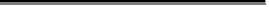
\includegraphics[width=0.48\textwidth,height=1.2mm]{garde/filet_noir}\\[4mm]
  \begin{minipage}{0.86\textwidth}
    \centering\fontsize{20}{24}\selectfont\bfseries \@title
  \end{minipage}\\[4mm]
  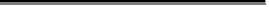
\includegraphics[width=0.48\textwidth,height=1.2mm]{garde/filet_noir}

  \vspace{14mm}
  {\fontsize{11}{13}\selectfont\bfseries Soutenue le : 17/10/2026}\\[2mm]
  {\fontsize{11}{13}\selectfont\bfseries Devant le jury composé de :}

  \vspace{6mm}
  {\fontsize{12}{14}\selectfont\bfseries
  \begin{tabular}{@{}l@{\hspace{2mm}}l@{}}
    Président : & Dr. Emna Khanfir\\[2mm]
    Rapporteur : & Dr. Ahmed Dridi\\[2mm]
    Encadrant académique : & \@academicFramerName\\[2mm]
    Encadrante professionnelle : & \@proFramerName
  \end{tabular}}

  \vfill
  {\fontsize{11}{13}\selectfont\bfseries Année Universitaire : 2025-2026}
\end{center}
}

% The blank verso only matters for the printed copy (colour cover followed by
% the black-and-white cover); see \printversiontrue in main.tex.
\ifprintversion\afterpage{\blankpage}\fi

        \ifprintversion
            \clearpage
            
%===== File containing the black cover of the document ====%
%                                                          %
% Copyright (C) ISI - All Rights Reserved                  %
% Proprietary                                              %
% Written by Med Hossam <med.hossam@gmail.com>, April 2016 %
%                                                          %
% @author: HEDHILI Med Houssemeddine                       %
% @linkedin: http://tn.linkedin.com/in/medhossam           %
%==========================================================%

%== It's advised to not modify the content of this file ===%
% To set your information, go to global_config.tex file    %
%==========================================================%

\thispagestyle{cover}%
\hspace{-47pt}
\begin{minipage}[l]{0.2\columnwidth}
\vspace{6mm}

\includegraphics[width=1.1\columnwidth]{Logo_ISI_Kef}\\
\end{minipage}
\hfill
\begin{minipage}[l]{0.6\columnwidth}
\centering
\footnotesize
\textbf{{République Tunisienne}}\\
\vspace{1.5mm}
\textbf{{Ministère de l'Enseignement Supérieur\\
et de la Recherche Scientifique}}\\
\vspace{1.5mm}
\textbf{{Université de Jendouba}}\\
\vspace{1.5mm}
\textbf{{Institut Supérieur d'Informatique du Kef}}
\end{minipage}
\hfill
\begin{minipage}[l]{0.02\columnwidth}
\end{minipage}
\hfill
\begin{minipage}[l]{0.18\columnwidth}
\vspace{6mm}

\includegraphics[width=0.9\columnwidth]{Logo_UJ}\\
\end{minipage}
\vskip1.5cm

\begin{center}
{\LARGE{\textbf{\textsc{Rapport de Projet de Fin d'\'Etudes}}}}\\
\vskip0.5cm
\large

{\textbf{Présenté en vue de l'obtention du}}\\
\vskip2mm
{\textbf{\@diplomaName}}\\
{\textbf{Spécialité : \@speciality}}\\
{}
\end{center}

\begin{center}
\textrm{Par}\\
\vskip0.3cm
{\ifthenelse{\boolean{isBinomal}}
    {% IF TRUE
        \begin{center}
            \large\textbf{\@author}~~~~~ et ~~~~~
            \large\textbf{\@secondAuthor}
        \end{center}
    }
    {\Large\textbf{\@author}}% FALSE
}
\vskip12mm

\begin{changemargin}{-9mm}{0cm}
\begin{minipage}[l]{1.1\columnwidth}
\begin{tcolorbox}[colback=white,boxrule=0pt,toprule=3pt,bottomrule=3pt,arc=0pt,top=0mm,right=0mm,left=0mm,bottom=0mm,boxsep=0.5mm]{
    \begin{tcolorbox}[colback=white, boxrule=0pt,toprule=1pt,bottomrule=1pt,arc=0pt,enlarge bottom by=-0.9mm, auto outer arc]
        \centering
        {\huge\textbf{\@title}}
    \end{tcolorbox}
}
\end{tcolorbox}
\end{minipage}
\end{changemargin}

\end{center}
\vskip8mm%

\begin{center}
\large
\begin{tabular}{r@{\hspace{12mm}}l}
Encadrante professionnelle : & \textbf{\@proFramerName}\\[2mm]
Encadrant académique : & \textbf{\@academicFramerName}
\end{tabular}
\end{center}
\vskip10mm

\begin{center}
\large
Réalisé au sein de \@companyName\\
\vskip0.4cm
{{\fboxrule=1.5pt\fbox{
\includegraphics[width=0.18\columnwidth]{Logo_CyberCloud}}}}\par
\end{center}

\restoregeometry

        \fi
        \clearpage
        \thispagestyle{empty}

\begin{center}
    \begin{minipage}[l]{1\columnwidth}
        \begin{tcolorbox}[colback=white,boxrule=5pt,arc=10pt,height=105mm]{
            \vspace{2cm}
            \large \@proSignSentence
            \vspace{1mm}
            \begin{center}
                \Large
                Encadrante professionnelle, \textbf{\@proFramerName}
            \end{center}
            \vspace{5mm}
            \hspace{0.71\columnwidth}\textbf{\large Signature et cachet}
        }
        \end{tcolorbox}
    \end{minipage}
    
    \vspace{2cm}
    
    \begin{minipage}[l]{1\columnwidth}
        \begin{tcolorbox}[colback=white,boxrule=5pt,arc=10pt,height=105mm]{
            \vspace{2cm}
            \large \@academicSignSentence
            \vspace{1mm}
            \begin{center}
                \Large
                Encadrant académique, \textbf{\@academicFramerName}
            \end{center}
            \vspace{5mm}
            \hspace{0.84\columnwidth}\textbf{\large Signature}
        }
        \end{tcolorbox}
    \end{minipage}
\end{center}

        \cleardoublepage
        \chapter*{Dédicaces}
\addcontentsline{toc}{chapter}{Dédicaces}
\markboth{Dédicaces}{}

\begin{center}
\begin{minipage}{0.83\textwidth}
\itshape
C’est avec une profonde gratitude et des mots sincères que je dédie ce modeste travail.

\medskip
\textbf{À mes chers parents, Abedlwaheb El Ech et Habiba Omri.} Votre soutien indéfectible et votre amour inconditionnel ont été une source inestimable de force et d’inspiration. Que ce travail soit le témoignage de ma profonde reconnaissance et de ma gratitude infinie. Que Dieu vous bénisse, vous accorde santé et longue vie.

\medskip
\textbf{À ma petite sœur, Hayfa El Ech.} Merci pour ton soutien, ta présence et tes encouragements tout au long de ce parcours.

\medskip
\textbf{À ma famille.} Je vous remercie pour votre affection, votre confiance et votre soutien constant.

\medskip
\textbf{À mes amis.} Pour tous les instants inoubliables que nous avons passés ensemble, je vous remercie du fond du cœur. Que ce travail soit également le témoignage de mon amitié et de ma reconnaissance pour votre soutien.
\end{minipage}
\end{center}

\vfill
\begin{flushright}
\textit{\Large El Ech Iheb}\\[-1mm]
\rule{4.5cm}{0.35pt}
\end{flushright}

        \cleardoublepage
        \chapter*{Remerciements}
\addcontentsline{toc}{chapter}{Remerciements}
\markboth{Remerciements}{}

Je remercie Dieu le Tout-Puissant de m’avoir donné la santé et la volonté d’entamer et de terminer ce rapport.

J’exprime également ma sincère gratitude à mon encadrant à l’ISI Kef, \textbf{Dr. Aymen Louati}, pour son aide et ses conseils concernant l’acheminement du projet et l’architecture du rapport. Je le remercie pour le temps qu’il m’a consacré, pour les informations qu’il m’a fournies avec compréhension, ainsi que pour sa patience et son amabilité.

J’adresse également mes remerciements à \textbf{Dr. Emna Trabelsi} pour sa pédagogie, sa confiance et le soutien qu’elle m’a accordé tout au long de ce projet au sein de CyberCloud Solutions.

Je tiens de même à remercier tous les enseignants de l’ISI Kef qui m’ont enseigné pendant ces trois années successives et qui, par leurs compétences, m’ont soutenu dans la poursuite de mes études.

Enfin, je présente mes profonds remerciements et mon respect aux membres du jury qui ont accepté de juger mon travail.

        \cleardoublepage
        
        \setcounter{page}{1}
        \setcounter{secnumdepth}{3}
        \setcounter{tocdepth}{2}
        \markboth{\contentsname}{}
        \tableofcontents
        \thispagestyle{frontmatter}
        
        \cleardoublepage
        \markboth{\listfigurename}{}
        \listoffigures
        \thispagestyle{frontmatter}
        \cleardoublepage
        \markboth{\listtablename}{}
        \listoftables
        \thispagestyle{frontmatter}
        \cleardoublepage
        \chapter*{Liste des abréviations}
\addcontentsline{toc}{chapter}{Liste des abréviations}
\markboth{Liste des abréviations}{}

% Les trois minipages de \sortitem occupent 1,00\columnwidth et sont placees
% dans un itemize : la somme deborde de la valeur du retrait de liste. On reduit
% localement la largeur de reference pour que chaque ligne tienne dans la marge.
{\setlength{\columnwidth}{\dimexpr\columnwidth-40pt\relax}
\begin{acronyms}
  \sortitem[API]{Interface de programmation applicative}
  \sortitem[ASGI]{Interface asynchrone entre un serveur Web et une application Python}
  \sortitem[ATS]{Système de suivi des candidatures}
  \sortitem[AUC]{Aire sous la courbe}
  \sortitem[BERT]{Modèle de représentation contextuelle bidirectionnelle du texte}
  \sortitem[CPU]{Processeur central}
  \sortitem[CRUD]{Créer, lire, mettre à jour et supprimer}
  \sortitem[CSS]{Feuilles de style en cascade}
  \sortitem[CSV]{Fichier texte de valeurs séparées par des virgules}
  \sortitem[CV]{Curriculum vitae}
  \sortitem[DevOps]{Pratiques associant développement et exploitation}
  \sortitem[DOCX]{Format de document Word fondé sur XML}
  \sortitem[HTTP]{Protocole de transfert hypertexte}
  \sortitem[HTTPS]{Protocole de transfert hypertexte sécurisé par TLS}
  \sortitem[IA]{Intelligence artificielle}
  \sortitem[IP]{Protocole Internet, et par extension l'adresse qu'il attribue}
  \sortitem[JSON]{Format d'échange de données textuel}
  \sortitem[JWT]{JSON Web Token}
  \sortitem[LLM]{Grand modèle de langage}
  \sortitem[LTS]{Version bénéficiant d'un support à long terme}
  \sortitem[NSG]{Network Security Group}
  \sortitem[OAuth2]{Protocole de délégation d'autorisation, utilisé ici pour le formulaire de connexion}
  \sortitem[ORM]{Correspondance objet--relationnel}
  \sortitem[OWASP]{Open Worldwide Application Security Project}
  \sortitem[PDF]{Portable Document Format}
  \sortitem[RAM]{Mémoire vive}
  \sortitem[RH]{Ressources humaines}
  \sortitem[ROC]{Courbe caractéristique de fonctionnement du récepteur}
  \sortitem[SQL]{Langage de requête structuré pour bases relationnelles}
  \sortitem[SSD]{Disque à mémoire flash}
  \sortitem[SSH]{Protocole d'accès distant sécurisé à une machine}
  \sortitem[TCP]{Protocole de transport en mode connecté}
  \sortitem[TF--IDF]{Term Frequency--Inverse Document Frequency}
  \sortitem[TLS]{Protocole de chiffrement des échanges réseau}
  \sortitem[UFW]{Pare-feu en ligne de commande d'Ubuntu}
  \sortitem[UML]{Unified Modeling Language}
  \sortitem[URL]{Adresse d'une ressource sur le Web}
  \sortitem[VM]{Machine virtuelle}
  \sortitem[WAF]{Pare-feu applicatif Web}
  \sortitem[XDR]{Détection et réponse étendues aux incidents de sécurité}
  \sortitem[XML]{Langage de balisage extensible}
  \sortitem[XSS]{Injection de script dans une page Web}
\end{acronyms}
}

        \cleardoublepage
        % Les quatre chapitres non numérotés précédents ont une entrée dans la table des matières.
        % Cet ajustement aligne minitoc avec les fichiers de plans générés.
        \setcounter{mtc}{4}
        
    \mainmatter
        \chapter*{Introduction générale}
\addcontentsline{toc}{chapter}{Introduction générale}
\markboth{Introduction générale}{}

Le recrutement exige d'examiner des CV nombreux et hétérogènes au regard d'offres dont les exigences sont souvent formulées de manière libre. Cette première lecture mobilise du temps, tout en devant rester justifiable et attentive au contexte de chaque candidature. Une assistance logicielle peut organiser les informations utiles, mais elle ne peut pas se substituer au jugement du recruteur ni produire seule une décision d'embauche.

Ce mémoire présente \textit{JobTest}, réalisé dans le cadre du stage de PFE chez CyberCloud Solutions. Le projet répond au besoin d'une aide à la présélection qui rapproche un CV et une offre, rend visibles les éléments de correspondance et conserve les résultats d'évaluation. La plateforme permet au recruteur de gérer ses offres et ses candidats, de lancer des évaluations sur du texte ou des documents, puis de consulter un résultat composé d'un score, de sous-scores, de compétences détectées, d'écarts et de recommandations.

La solution associe une couche déterministe fondée sur TF--IDF, la similarité sémantique et les compétences, à une politique de décision explicite. Une analyse qualitative locale peut compléter la restitution, sans modifier le verdict officiel. L'application s'appuie sur un frontend Next.js, une API FastAPI, une persistance relationnelle et un export PDF. Les validations documentées couvrent les parcours principaux, un benchmark sur données synthétiques et un déploiement de démonstration conteneurisé sur Microsoft Azure.

Le premier chapitre présente le contexte, l'organisme d'accueil, la problématique et la démarche. Le deuxième précise les besoins et les règles de gestion. Le troisième expose la conception fonctionnelle et architecturale. Le quatrième décrit le moteur d'évaluation et son protocole expérimental. Le cinquième présente la réalisation de la plateforme, tandis que le sixième traite des tests, de la sécurité, de l'industrialisation et du déploiement. La conclusion générale synthétise les apports, les limites et les perspectives de JobTest.

        \clearpage
        \chapter{Contexte général et étude préalable}

\section*{Introduction}
Le présent chapitre fixe le cadre organisationnel, fonctionnel et méthodologique du projet \textit{JobTest}. Il situe d'abord le stage au sein de CyberCloud Solutions, puis examine le problème de présélection de CV et les réponses actuellement proposées par les outils numériques. Cette étude préalable sert à délimiter précisément la contribution de JobTest : une aide à l'analyse et à la comparaison de candidatures, et non un mécanisme autonome de recrutement. Le chapitre formule ensuite la problématique, décrit la solution retenue, ses objectifs ainsi que la démarche de conduite du projet.

\section{Présentation de l'organisme d'accueil}

\subsection{Présentation de CyberCloud Solutions}
CyberCloud Solutions est une entreprise de services et de conseil en informatique fondée en 2017. Sa page publique la situe dans le Grand Tunis, indique un effectif de deux à dix personnes et présente une organisation tournée vers l'accompagnement technique, le conseil et la transformation numérique \cite{cybercloud_linkedin}. Dans ce contexte, l'entreprise peut réunir des besoins variés autour des environnements numériques sans que cela implique une spécialisation unique sur le recrutement.

Son positionnement associe prestation de services, assistance et conseil. La flexibilité du travail à distance ou hybride est cohérente avec le cadre du stage décrit dans ce mémoire : elle permet de structurer un travail individuel autour de livrables partagés et vérifiables, sans présumer d'une organisation interne, d'un rythme de réunion ou d'une répartition de services qui ne sont pas documentés publiquement.

La figure \ref{fig:cybercloud-logo} reproduit le logo employé par l'entreprise sur sa page officielle. Il est utilisé ici uniquement pour identifier l'organisme d'accueil.

\begin{figure}[htbp]
  \centering
  
\includegraphics[width=0.26\textwidth]{Logo_CyberCloud}
  \caption{Logo de CyberCloud Solutions (source : page officielle de l'entreprise \cite{cybercloud_linkedin})}
  \label{fig:cybercloud-logo}
\end{figure}

\subsection{Activités et domaines d'expertise}
Les activités publiées par CyberCloud Solutions peuvent être regroupées sans les confondre avec le périmètre de JobTest. Un premier ensemble concerne le conseil, l'assistance et la transformation numérique. Un deuxième porte sur l'infrastructure : équipements informatiques et bureautiques, serveurs, stockage, postes de travail, imprimantes et logiciels professionnels. La présentation publique mentionne également des solutions de sécurité Internet, de \textit{network forensics} et d'interception légale \cite{cybercloud_linkedin}.

Les spécialités affichées complètent ce panorama : cybersécurité, XDR, réseaux, serveurs, cloud, DevOps, logiciels et intelligence. Elles montrent un environnement technique pluridisciplinaire ; elles ne signifient pas que chacun de ces domaines a été directement mobilisé pour la plateforme. JobTest relève plus précisément de l'ingénierie d'une application d'aide au recrutement, à l'intersection du traitement de texte, du développement web, de la persistance des données et de l'évaluation de modèles.

\subsection{Cadre du stage}
Ce projet est réalisé par Iheb El Ech dans le cadre du Mastère Professionnel en Applications Web Intelligentes de l'Institut Supérieur d'Informatique du Kef, relevant de l'Université de Jendouba, pour l'année universitaire 2025--2026. Le stage de PFE s'étend de mars à août 2026. Le sujet, proposé par CyberCloud Solutions, est : \emph{conception et développement d'une plateforme intelligente d'aide au recrutement et de mise en correspondance entre CV et offres d'emploi}.

L'étudiant intervient individuellement en qualité de stagiaire PFE, dans un mode principalement distant ou hybride. L'encadrement professionnel est assuré par Dr. Trabelsi Emna. Ce cadre précise l'origine professionnelle du besoin tout en conservant le caractère académique du travail : les choix techniques, les résultats et leurs limites doivent pouvoir être explicités et contrôlés.

\section{Contexte du projet}
Une candidature condense des informations de natures différentes : expériences, formations, compétences déclarées, réalisations, certifications et éléments libres. Les offres d'emploi présentent elles aussi des exigences hétérogènes, parfois sous forme de listes, parfois dans des descriptions rédigées. La généralisation des candidatures en ligne a accru le volume à examiner et rend la présélection plus difficile à organiser manuellement \cite{ilo_hrm_2026}.

L'intelligence artificielle désigne notamment des systèmes capables de produire des prédictions, recommandations ou décisions pour des objectifs définis par des humains \cite{nist_ai}. Dans le cas du recrutement, cette capacité ne retire ni la responsabilité ni le jugement professionnel du recruteur. Les travaux sur les outils algorithmiques de ressources humaines soulignent à la fois leur intérêt pour traiter de nombreux dossiers et les risques de biais, d'opacité ou de mauvaise interprétation qui justifient une supervision humaine \cite{koechling2020fairness,ilo_hrm_2026}.

Une recherche par mots-clés est utile pour repérer des termes explicitement demandés, mais elle ne traite pas toujours les formulations proches, les synonymes ou les compétences décrites indirectement. La représentation contextuelle des textes a précisément été développée pour mieux exploiter le contexte linguistique \cite{devlin2019bert}. Des représentations de phrases comparables par similarité cosinus permettent, par exemple, de rapprocher deux textes sur une base sémantique plutôt que de compter seulement des mots identiques \cite{reimers2019sbert}. Pour la présélection, l'enjeu n'est donc pas de remplacer le recruteur, mais de fournir un résultat reproductible, décomposé et intelligible : ce qui concorde, ce qui manque et ce qui a conduit à une recommandation.

\section{Étude de l'existant}

\subsection{Processus manuel de présélection}
Dans un processus manuel, le recruteur lit l'offre, définit ses critères, ouvre les CV, repère les expériences et compétences pertinentes, puis conserve ou écarte des candidatures avant les étapes suivantes. Cette séquence laisse place à une appréciation qualitative indispensable, notamment pour interpréter un parcours atypique ou contextualiser une expérience.

Elle devient cependant coûteuse à répéter lorsque les documents sont nombreux et de formats disparates. Elle rend également plus difficile la traçabilité du raisonnement appliqué à chaque dossier. La littérature consacrée aux décisions algorithmiques en ressources humaines rappelle que la recherche d'efficacité ne constitue pas, à elle seule, une garantie d'équité : la définition des critères, la qualité des données et le contrôle humain restent déterminants \cite{koechling2020fairness}. JobTest ne cherche donc pas à transformer une préconisation en décision d'embauche ; il structure l'examen initial et rend visibles ses éléments de calcul.

\subsection{Approches lexicales et ATS traditionnels}
Les systèmes de suivi de candidatures (\textit{Applicant Tracking Systems}, ou ATS) organisent habituellement les offres, les profils candidats, les étapes de pipeline et les évaluations. Dans ce type d'environnement, la recherche peut s'appuyer sur des mots, des étiquettes, des filtres ou des champs structurés. Cette approche est efficace quand l'exigence est explicitement formulée et que la terminologie est stable. Elle devient moins robuste lorsqu'une compétence est exprimée par une paraphrase, lorsque le CV est multilingue ou lorsqu'une expérience pertinente ne reprend pas le vocabulaire exact de l'offre.

L'analyse textuelle par termes demeure ainsi un signal, non une preuve complète d'adéquation. Les revues sur le recrutement assisté indiquent que les outils de sélection vont aujourd'hui de la recherche de mots à des traitements cherchant des correspondances plus contextuelles ; elles invitent également à distinguer le filtrage technique de la validité d'une décision de sélection \cite{koechling2020fairness}. La comparaison sémantique et l'analyse explicite des compétences constituent donc des compléments pertinents, à condition que leurs résultats restent contrôlables.

\subsection{Solutions numériques étudiées}
Trois solutions ont été retenues pour une comparaison ciblée, à partir de leur documentation officielle consultée le 13 septembre 2026. LinkedIn Recruiter propose une recherche assistée par IA à partir d'une demande en langage naturel ; selon l'offre et la langue, elle peut produire des recommandations et une synthèse expliquant l'adéquation affichée sur la carte d'un candidat \cite{linkedin_recruiter_search,linkedin_recruiter_ai}. La documentation étudiée ne permet pas de conclure à la présence d'une analyse détaillée des lacunes de compétences ni d'un export de rapport de correspondance CV/offre.

Workable centralise les profils, les CV et le pipeline. Sa vue de candidature permet notamment une recherche par mots-clés ou recherche avancée, l'affichage des compétences et le tri par meilleure évaluation ou meilleur appariement fondé sur les évaluations IA \cite{workable_pipeline}. Sa documentation de sécurité mentionne des dispositifs de protection des données, dont le chiffrement en transit, des mécanismes liés aux droits des candidats et des contrôles de conformité \cite{workable_security}. Ces informations décrivent la plateforme Workable, pas le niveau de protection d'une installation particulière.

Greenhouse Recruiting documente une fonction \emph{Talent Matching} qui compare les CV à une calibration définie et pondérée pour le poste. Il propose aussi des \textit{scorecards} pour évaluer les candidats selon des critères préparés, ainsi que des rapports candidats exportables au format tableur \cite{greenhouse_ai,greenhouse_scorecards,greenhouse_reports}. Les sources consultées ne documentent pas un diagnostic autonome de lacunes de compétences comparable à celui visé par JobTest.

\subsection{Synthèse comparative}
Le tableau \ref{tab:comparatif-existant} met en regard des capacités directement documentées. Il ne mesure ni la qualité réelle de chaque solution, ni leur couverture complète : la mention \emph{non documenté} signifie seulement qu'aucune preuve explicite n'a été trouvée dans les pages officielles consultées. Les informations sur JobTest proviennent du code, des rapports techniques du dépôt et du déploiement vérifié du projet.

\begin{table}[htbp]
\centering
\scriptsize
\setlength{\tabcolsep}{3pt}
\renewcommand{\arraystretch}{1.28}
\begin{tabularx}{\textwidth}{|p{0.20\textwidth}|X|X|X|X|}
\hline
\textbf{Critère} & \textbf{LinkedIn Recruiter} & \textbf{Workable} & \textbf{Greenhouse Recruiting} & \textbf{JobTest}\\
\hline
Correspondance CV/offre & Recherche IA et recommandations à partir d'une demande ; synthèse de fit selon disponibilité & Tri \emph{best match} issu d'évaluations IA ; CV dans le pipeline & Talent Matching : CV comparé à une calibration pondérée & Analyse hybride : lexical, sémantique et compétences\\
\hline
Éléments explicatifs & Synthèse IA de fit pour certains accès ; granularité non documentée & Évaluation et score visibles ; décomposition d'IA non documentée & Scorecards structurées et critères d'entretien & Scores composantes, compétences, écarts et recommandations\\
\hline
Analyse des écarts de compétences & Non documenté & Non documenté & Non documenté & Compétences correspondantes, manquantes et critiques\\
\hline
Classement et export & Résultats de recherche ; export de rapport d'appariement non documenté & Tri de candidats ; export de rapport d'appariement non documenté & Rapport candidat exportable en XLS & Classement multi-CV, historique et rapport PDF\\
\hline
Contrôle et données & Modèle de déploiement/confidentialité non documenté dans les sources consultées & Documentation sécurité et confidentialité disponible & Modèle de déploiement/confidentialité non documenté dans les sources consultées & Persistance limitée au recruteur ; déploiement PFE sur VM Azure\\
\hline
\end{tabularx}
\caption{Comparaison fonctionnelle fondée sur les documentations officielles consultées \cite{linkedin_recruiter_ai,workable_pipeline,workable_security,greenhouse_ai,greenhouse_scorecards,greenhouse_reports}}
\label{tab:comparatif-existant}
\end{table}

\section{Critique de l'existant}
Les plateformes étudiées couvrent des besoins opérationnels importants : recherche, pipeline, évaluation structurée, gestion de candidats et, selon les produits, fonctions d'IA. Elles ne sont donc pas des alternatives faibles à écarter ; elles répondent à des contextes organisationnels plus larges que le périmètre du PFE. La comparaison révèle surtout un besoin de cohérence entre l'analyse du texte, le contrôle de la règle de décision et l'explication fournie au recruteur.

JobTest adresse ce besoin par une chaîne unique : une analyse hybride associe un signal lexical, un signal sémantique et une analyse des compétences ; un moteur de décision central applique la même politique à toutes les interfaces ; les composantes, les compétences manquantes et des recommandations sont restituées avec le résultat. Les évaluations enregistrent également des métadonnées de reproductibilité, notamment la configuration de décision et les poids utilisés. Une analyse qualitative facultative, exécutée localement via Ollama, intervient après le score statistique et ne peut ni le modifier ni annuler la recommandation.

Cette proposition comporte des limites qu'il faut exposer dès maintenant. L'évaluation hors ligne repose sur des données synthétiques ; elle ne constitue donc pas une preuve de performance sur des décisions d'embauche réelles. L'inférence sémantique et la petite couche LLM locale sont exécutées sur CPU, ce qui introduit une latence perceptible pour l'analyse approfondie. Le déploiement Azure vérifié est adapté à une démonstration de PFE : il s'agit d'une instance unique, publiée en HTTP, sans dispositif de haute disponibilité. Enfin, le petit modèle local peut produire une analyse superficielle ou inexacte ; son résultat est strictement consultatif. Ces limites renforcent la nécessité d'un recruteur décisionnaire.

\section{Problématique}
La problématique du projet peut être formulée ainsi :

\begin{quote}
\emph{Comment fournir au recruteur, à partir d'un CV et d'une offre d'emploi, une évaluation hybride de la proximité sémantique et des compétences qui soit explicable, reproductible et persistante, tout en préservant une analyse qualitative consciente de ses limites et sans déléguer la décision d'embauche à l'outil ?}
\end{quote}

Cette question associe quatre exigences. Il faut traiter le contenu hétérogène des documents, rendre la recommandation vérifiable par ses composantes, conserver le contexte nécessaire à la reproductibilité et encadrer l'usage d'une analyse générative par une approche respectueuse des données et du rôle du recruteur.

\section{Solution proposée : JobTest}
JobTest est une plateforme web d'aide au recrutement destinée au recruteur ou spécialiste RH. Elle permet de créer et gérer des offres, de saisir le texte d'un CV ou de téléverser un document PDF ou DOCX, puis de lancer une évaluation contre une offre sélectionnée. Le résultat comprend une recommandation \texttt{HIRE}, \texttt{CONSIDER} ou \texttt{REJECT}, un score global, une décomposition des composantes et une présentation des compétences détectées, correspondantes ou absentes.

La plateforme complète l'analyse individuelle par la gestion des candidats et de l'historique, un classement de plusieurs CV pour une même offre, ainsi qu'un rapport PDF. Elle met aussi à disposition une comparaison de modèles et un \textit{AI Quality Center} qui expose un benchmark hors ligne avec sa provenance. Ces éléments distinguent une aide au recrutement instrumentée d'une simple recherche textuelle.

Une analyse approfondie optionnelle est disponible via un modèle local exécuté par Ollama. Elle produit une lecture qualitative, des points d'attention, des recommandations et des questions d'entretien. Elle est appelée après la couche statistique ; elle est donc additionnelle. La décision et le score officiels restent issus du moteur déterministe de la plateforme. Les données métier sont isolées par recruteur, et les résultats d'analyse sont conservés afin de pouvoir les retrouver dans le workflow.

\section{Objectifs du projet}

\subsection{Objectif général}
L'objectif général est de concevoir et développer une plateforme d'aide à la présélection qui aide un recruteur à comparer des CV à une offre de façon structurée, explicable et reproductible, sans automatiser la décision d'embauche.

\subsection{Objectifs spécifiques}
Les objectifs spécifiques retenus sont les suivants :

\begin{itemize}[leftmargin=15mm]
  \item mettre en oeuvre un workflow de recrutement comprenant l'authentification, la gestion des offres et la gestion des candidats ;
  \item accepter un CV sous forme de texte saisi ou de document PDF/DOCX ;
  \item associer des signaux lexicaux, sémantiques et orientés compétences dans une même évaluation ;
  \item appliquer une politique de décision cohérente pour les recommandations \texttt{HIRE}, \texttt{CONSIDER} et \texttt{REJECT} ;
  \item exposer les composantes du score, les compétences correspondantes, les écarts et des recommandations d'amélioration ;
  \item enregistrer les évaluations, leurs paramètres utiles et l'historique associé au recruteur ;
  \item générer un rapport PDF et proposer un classement de plusieurs candidatures pour une offre ;
  \item comparer les méthodes disponibles et afficher les résultats d'une évaluation hors ligne avec leur provenance ;
  \item intégrer des mesures de sécurité applicative, notamment l'authentification et le cloisonnement des données par recruteur ;
  \item déployer une version démontrable de la solution avec le frontend, l'API, la base de données et la couche d'analyse locale.
\end{itemize}

\section{Méthodologie de conduite du projet}

\subsection{Justification du modèle en cascade}
Le modèle en cascade organise un projet logiciel en séquences identifiables, depuis l'expression du besoin jusqu'à la validation. Dans son article fondateur, Royce insiste sur la documentation et sur la nécessité de retours contrôlés lorsque les résultats d'une phase révèlent un problème \cite{royce1970}. Il ne doit donc pas être interprété comme une interdiction absolue de corriger l'implémentation.

Pour JobTest, ce cadre convient à un PFE dont les livrables attendus peuvent être stabilisés : besoins, conception, réalisation, tests et déploiement. Il fournit un fil de lecture clair pour le mémoire et la démonstration. Des corrections techniques et des retours de validation ont néanmoins été réalisés à l'intérieur des phases d'implémentation et de validation, notamment sur la cohérence de la décision, l'analyse des compétences, la qualité du benchmark et la sécurisation des accès. Le modèle en cascade décrit ici la progression principale ; il ne masque pas ces boucles de correction.

\subsection{Phases appliquées à JobTest}
La figure \ref{fig:waterfall-jobtest} présente la déclinaison de cette démarche pour JobTest. Chaque étape produit un résultat qui alimente la suivante, tandis que la phase de validation peut conduire à corriger le livrable concerné.

\begin{figure}[htbp]
  \centering
  \begin{tikzpicture}[
  node distance=4mm,
  phase/.style={
    rectangle, rounded corners=2pt, draw=isiBlue, very thick,
    fill=blue!7, minimum width=0.76\textwidth, minimum height=8.5mm,
    align=center, font=\small\bfseries
  },
  arrow/.style={-{Stealth[length=2.2mm]}, very thick, draw=isiBlue}
]
  \node[phase] (needs) {1. Recueil et formalisation des besoins};
  \node[phase, below=of needs] (analysis) {2. Analyse};
  \node[phase, below=of analysis] (design) {3. Conception};
  \node[phase, below=of design] (build) {4. Implémentation};
  \node[phase, below=of build] (validate) {5. Validation et correction};
  \node[phase, below=of validate] (deploy) {6. Déploiement};
  \draw[arrow] (needs) -- (analysis);
  \draw[arrow] (analysis) -- (design);
  \draw[arrow] (design) -- (build);
  \draw[arrow] (build) -- (validate);
  \draw[arrow] (validate) -- (deploy);
  \draw[-{Stealth[length=2.2mm]}, dashed, thick, draw=gray]
    (validate.east) to[out=0,in=0,looseness=1.15] node[right, font=\scriptsize, align=left]
    {retours de\\correction} (build.east);
\end{tikzpicture}

  \caption{Déroulement en cascade adapté au projet JobTest}
  \label{fig:waterfall-jobtest}
\end{figure}

Le recueil et la formalisation des besoins ont permis de préciser le rôle du recruteur, les entrées CV/offre et les attentes d'explication. L'analyse a ensuite structuré les cas d'usage, les données manipulées et les contraintes de confidentialité. La conception a défini la séparation entre interface web, API, moteur d'appariement, décision, persistance et analyse qualitative optionnelle.

L'implémentation a produit l'application web, les services de traitement des CV, la gestion des offres et des candidats, l'export PDF et les écrans d'évaluation. La validation a porté sur les parcours fonctionnels, le classement, les rapports, les résultats d'évaluation et les corrections du moteur. Enfin, le déploiement a rassemblé Next.js, FastAPI, PostgreSQL, Ollama et Nginx dans une configuration Docker Compose sur une machine virtuelle Azure. Cette dernière étape reste une livraison de démonstration, avec les limites d'exploitation déjà indiquées.

\section*{Conclusion}
Ce chapitre a présenté CyberCloud Solutions, le cadre individuel du stage et les contraintes du problème de présélection. L'étude de l'existant a montré l'intérêt des ATS et de l'assistance par IA, tout en mettant en évidence l'importance de l'explicabilité, de la supervision humaine et de la prudence face aux résultats automatisés. JobTest répond à ce besoin par une analyse hybride, une décision cohérente et une restitution orientée recruteur, tout en assumant les limites de ses données, de ses modèles et de son déploiement. Le chapitre suivant, \emph{Analyse et spécification des besoins}, détaillera les acteurs, les besoins fonctionnels et non fonctionnels ainsi que la spécification du système.

        \clearpage
        \chapter{Analyse et spécification des besoins}

\section*{Introduction}
L'analyse des besoins transforme le périmètre présenté au chapitre précédent en attentes vérifiables, cas d'utilisation et règles de gestion. Elle s'appuie ici sur le comportement du dépôt JobTest : interface Next.js, routes FastAPI effectivement sollicitées, persistance et moteur de décision. L'objectif n'est pas de décrire une plateforme RH générique, mais de fixer le contrat fonctionnel de l'application démontrable. Après la délimitation du système et l'identification de ses parties prenantes, le chapitre spécifie les besoins, les contraintes de qualité, les règles de gestion, les cas d'utilisation et leur traçabilité.

\section{Périmètre fonctionnel de JobTest}
JobTest est une application d'aide à la présélection destinée au recruteur. Elle organise des offres et des dossiers candidats, puis fournit une évaluation hybride entre un CV et une offre. Le résultat associe une recommandation officielle, ses composantes, les compétences détectées ou manquantes et des éléments d'explication. L'analyse qualitative produite par le LLM local complète cette restitution sans participer à la décision officielle.

Le périmètre couvert comprend l'inscription et la session du recruteur, la gestion des offres et des candidats, l'évaluation d'un texte ou d'un document PDF/DOCX, la consultation des résultats et de l'historique, le classement multi-CV, l'export PDF, la comparaison ponctuelle des méthodes, le centre de qualité hors ligne et le réglage de seuils pour la session. Les données opérationnelles et les résultats persistés sont isolés par recruteur.

Sont hors périmètre une décision d'embauche autonome, un portail candidat, la conduite des entretiens et un apprentissage sur des résultats réels d'embauche. JobTest ne remplace donc pas l'appréciation du recruteur ni les étapes humaines de sélection. Son benchmark repose sur des données synthétiques. Enfin, le déploiement Azure validé est une démonstration PFE sur une instance sans haute disponibilité permanente ; il ne constitue pas une offre de production 24/7.

\section{Identification des acteurs et parties prenantes}
\subsection{Visiteur non authentifié}
Avant l'authentification, le visiteur peut créer un compte recruteur ou se connecter. Aucun parcours public de consultation d'offres, de dépôt de candidature, de réinitialisation de mot de passe, de vérification d'e-mail ou de connexion sociale n'a été retenu, car il n'est pas exposé par l'application actuelle.

\subsection{Recruteur authentifié}
Le recruteur est l'acteur opérationnel principal. Une fois la session JWT établie, il consulte le tableau de bord et gère ses propres offres, candidats et résultats. Il peut évaluer un CV, consulter le résultat explicable, demander l'analyse approfondie facultative, exporter un rapport, classer plusieurs CV, consulter l'historique, comparer les méthodes, visualiser la qualité hors ligne et modifier les seuils actifs de sa session. Les contrôles d'appartenance empêchent l'accès aux objets d'un autre recruteur.

\subsection{Candidat en tant qu'entité métier}
Le candidat est le sujet d'une évaluation et une entité persistée : identité facultative, coordonnées, statut de pipeline, CV et résultats associés. Il n'est pas un acteur logiciel interactif. La version étudiée ne fournit ni compte candidat ni écran candidat ni soumission publique de CV. Cette séparation évite de confondre l'objet métier évalué avec l'utilisateur autorisé à utiliser l'application.

\subsection{Partie prenante technique}
Une personne chargée de maintenance ou d'assurance qualité peut exécuter le benchmark hors ligne, exporter ses figures ou intervenir sur l'environnement. Cette partie prenante est technique et secondaire : aucun portail administrateur, rôle d'administration distinct ni parcours d'authentification administrateur n'est prouvé dans l'interface opérationnelle. Elle ne figure donc pas comme acteur du diagramme global.

Le tableau~\ref{tab:acteurs-jobtest} récapitule ces acteurs et situe chacun d'eux par rapport au parcours métier.

\begin{table}[htbp]
\centering\small
\begin{tabularx}{\textwidth}{|p{3.2cm}|p{2.5cm}|X|p{3.1cm}|}
\hline
\textbf{Élément} & \textbf{Type} & \textbf{Rôle} & \textbf{Accès au système}\\
\hline
Visiteur non authentifié & Acteur & Crée un compte ou amorce une session & Écran d'accès, sans données métier\\
\hline
Recruteur authentifié & Acteur & Gère et évalue ses dossiers & Toutes les fonctions métier après JWT\\
\hline
Candidat & Entité métier & Porte le CV, le pipeline et les résultats & Aucun accès interactif\\
\hline
Maintenance / QA & Partie prenante technique & Produit ou contrôle le benchmark hors ligne & Hors parcours métier courant\\
\hline
\end{tabularx}
\caption{Acteurs et parties prenantes de JobTest}
\label{tab:acteurs-jobtest}
\end{table}

\section{Spécification des besoins fonctionnels}
Les besoins sont présentés par domaine afin de décrire le parcours réellement disponible, sans confondre les fonctions du recruteur avec une décision autonome de recrutement.


Le tableau~\ref{tab:besoins-fonctionnels} énumère ces besoins avec leur identifiant, l'acteur concerné et le critère qui permet d'en constater la réalisation.

{\footnotesize\setlength{\tabcolsep}{2pt}
\begin{longtable}{|>{\raggedright\arraybackslash\scriptsize}p{2.15cm}|>{\raggedright\arraybackslash}p{4.05cm}|>{\raggedright\arraybackslash}p{1.9cm}|>{\raggedright\arraybackslash}p{1.8cm}|>{\raggedright\arraybackslash}p{3.55cm}|}
\caption{Besoins fonctionnels de JobTest}\label{tab:besoins-fonctionnels}\\
\hline
\textbf{Identifiant} & \textbf{Besoin fonctionnel} & \textbf{Acteur} & \textbf{Priorité} & \textbf{Critère d'acceptation}\\
\hline
\endfirsthead
\hline
\textbf{Identifiant} & \textbf{Besoin fonctionnel} & \textbf{Acteur} & \textbf{Priorité} & \textbf{Critère d'acceptation}\\
\hline
\endhead
BF-AUTH-01 & Créer un compte recruteur avec nom, e-mail et mot de passe. & Visiteur & Essentiel & Un compte de rôle \texttt{recruiter} est créé ; un e-mail déjà utilisé est refusé.\\
\hline
BF-AUTH-02 & S'authentifier et récupérer l'utilisateur courant. & Visiteur & Essentiel & Les identifiants valides donnent un JWT bearer puis le profil \texttt{/auth/me}.\\
\hline
BF-AUTH-03 & Clore la session côté interface. & Recruteur & Essentiel & Le jeton local est supprimé lors de la déconnexion.\\
\hline
BF-JOB-01 & Créer et lister ses offres. & Recruteur & Essentiel & Titre et description sont exigés ; un code \texttt{JOB-YYYY-NNN} est attribué.\\
\hline
BF-JOB-02 & Modifier une offre possédée et son statut. & Recruteur & Essentiel & Les statuts admis sont \texttt{OPEN}, \texttt{ON\_HOLD} et \texttt{CLOSED}.\\
\hline
BF-JOB-03 & Basculer rapidement l'ouverture d'une offre. & Recruteur & Compl. & L'action dédiée alterne \texttt{OPEN} et \texttt{CLOSED}.\\
\hline
BF-JOB-04 & Supprimer une offre non évaluée. & Recruteur & Essentiel & La suppression est refusée si des évaluations sont liées ; l'offre peut alors être clôturée.\\
\hline
BF-CAND-01 & Consulter ses candidats. & Recruteur & Essentiel & La liste est filtrée par propriétaire et expose activité, meilleur score et statut.\\
\hline
BF-CAND-02 & Mettre à jour identité, contact et pipeline. & Recruteur & Essentiel & Nom obligatoire ; statuts admis : \texttt{NEW}, \texttt{UNDER\_REVIEW}, \texttt{SHORTLISTED}, \texttt{INTERVIEW}, \texttt{HIRED}, \texttt{REJECTED}.\\
\hline
BF-CAND-03 & Supprimer un candidat sans résultat lié. & Recruteur & Essentiel & Une suppression avec évaluation est refusée ; le recruteur peut modifier le statut du pipeline.\\
\hline
BF-EVAL-01 & Évaluer du texte CV contre une offre possédée. & Recruteur & Essentiel & Le CV contient au moins cinq mots ; méthode, score, décision et explication sont retournés et persistés.\\
\hline
BF-EVAL-02 & Évaluer un PDF ou DOCX. & Recruteur & Essentiel & Seuls PDF et DOCX sont acceptés ; un texte lisible est extrait avant l'évaluation.\\
\hline
BF-EVAL-03 & Afficher le résultat explicable. & Recruteur & Essentiel & Verdict \texttt{HIRE}/\texttt{CONSIDER}/\texttt{REJECT}, composantes, compétences, écarts, recommandations et données radar sont restitués.\\
\hline
BF-LLM-01 & Demander séparément une analyse approfondie. & Recruteur & Compl. & La requête cible un \texttt{MatchResult} possédé ; son état peut être \texttt{ok}, désactivé, indisponible ou en erreur.\\
\hline
BF-REPORT-01 & Générer et télécharger un rapport PDF depuis un résultat. & Recruteur & Compl. & Le navigateur reçoit un document PDF à partir du résultat et de son explication.\\
\hline
BF-RANK-01 & Classer plusieurs CV pour une offre. & Recruteur & Compl. & Des fichiers PDF/DOCX sont évalués pour une offre sélectionnée, puis ordonnés par score décroissant.\\
\hline
BF-RANK-02 & Exporter le classement courant. & Recruteur & Compl. & L'interface produit un CSV côté navigateur ; il ne crée pas un nouvel enregistrement métier.\\
\hline
BF-HIST-01 & Consulter l'historique et le détail d'une évaluation. & Recruteur & Essentiel & Les résultats propres au recruteur sont listés, filtrables et consultables par identifiant.\\
\hline
BF-QUALITY-01 & Comparer les méthodes en direct. & Recruteur & Compl. & \textit{AI Insights} compare les méthodes sur un CV/offre fourni sans persister de \texttt{MatchResult}.\\
\hline
BF-QUALITY-02 & Consulter le benchmark hors ligne. & Recruteur & Compl. & \textit{AI Quality Center} affiche des données et figures file-backed avec leur disponibilité.\\
\hline
BF-SETTINGS-01 & Configurer les seuils de décision de la session. & Recruteur & Compl. & Les seuils Strong Fit et Potential Fit sont validés, transmis aux évaluations ultérieures et conservés dans celles-ci.\\
\hline
\end{longtable}\par}
\normalsize

\subsection{Authentification du recruteur}
\begin{itemize}
  \item Créer un compte recruteur avec nom, e-mail et mot de passe, en refusant un e-mail déjà utilisé.
  \item Se connecter, consulter son profil courant et fermer la session côté interface.
\end{itemize}

L'inscription crée uniquement un recruteur. La connexion utilise le formulaire OAuth2 de l'API, qui retourne un jeton bearer. L'interface conserve ce jeton pour appeler \texttt{/auth/me} et les routes protégées ; la déconnexion l'efface côté client. Aucun besoin de réinitialisation de mot de passe ou d'activation n'est spécifié car ces parcours ne sont pas présents.

\subsection{Gestion des offres et des candidats}
\begin{itemize}
  \item Créer, consulter, modifier, clôturer ou rouvrir ses propres offres ; le code est attribué automatiquement.
  \item Supprimer une offre seulement lorsqu'aucune évaluation ne lui est liée ; une offre évaluée peut être clôturée.
  \item Consulter les candidats du recruteur, mettre à jour leurs informations et leur statut de pipeline, puis supprimer un dossier sans résultat associé.
\end{itemize}

Les offres sont créées avec un titre, une description, des compétences requises facultatives et un statut. Le code est calculé automatiquement. Toutes les opérations vérifient le recruteur propriétaire. Une offre liée à des évaluations ne peut pas être supprimée, afin de préserver la cohérence de l'historique. L'évaluation crée ou réutilise le dossier candidat lorsque les informations disponibles le permettent ; la page candidats sert ensuite à la consultation et à la mise à jour. Les fonctions exposées dans l'interface courante sont la modification et la suppression conditionnelle. L'API historique comporte une anonymisation, mais elle n'est pas présentée comme un parcours du frontend Next.js faute d'action correspondante vérifiée.

\subsection{Évaluation et restitution}
\begin{itemize}
  \item Évaluer un texte CV ou un document PDF/DOCX par rapport à une offre possédée.
  \item Consulter le verdict, le score, les composantes, les compétences, les écarts et les recommandations enregistrés.
  \item Demander séparément une analyse approfondie locale ; son indisponibilité ne modifie pas le verdict officiel.
  \item Générer et télécharger le rapport PDF d'une évaluation.
\end{itemize}

Le recruteur sélectionne une offre qu'il possède, saisit éventuellement identité et e-mail, puis transmet du texte ou un fichier. La couche statistique lance l'appariement choisi, le \textit{DecisionEngine} applique les seuils actifs et le service persiste un résultat. Le résultat visible comprend le score global, les sous-scores, la décision, l'explication, les compétences et les écarts. L'analyse approfondie est une seconde demande sur une évaluation déjà persistée. Si Ollama est désactivé, indisponible ou en erreur, l'état est retourné sans bloquer ni altérer le verdict statistique. Seule une enveloppe avec état \texttt{ok} est sauvegardée. Le rapport PDF, enfin, réutilise les données déjà calculées et n'ouvre pas un nouveau calcul de correspondance.

\subsection{Historique, classement et réglages}
\begin{itemize}
  \item Consulter l'historique et le détail des évaluations appartenant au recruteur.
  \item Classer plusieurs CV pour une offre, puis exporter le classement courant au format CSV.
  \item Comparer ponctuellement les méthodes, consulter les résultats du benchmark hors ligne et régler les seuils actifs de la session.
\end{itemize}

Le classement accepte plusieurs fichiers pour une seule offre et lance l'évaluation de chaque fichier avant de les trier par score décroissant ; l'export CSV est généré par le frontend. L'historique expose les résultats persistés du recruteur et leur détail. \textit{AI Insights} exécute une comparaison directe non persistante, tandis que \textit{AI Quality Center} présente un benchmark hors ligne : il ne doit pas être interprété comme une mesure d'exactitude de production en temps réel. Les seuils Strong Fit et Potential Fit sont configurés dans le navigateur et accompagnent les évaluations ultérieures de cette session ; ils doivent respecter \texttt{potential < strong}, et les résultats antérieurs gardent les seuils enregistrés.

\section{Spécification des besoins non fonctionnels}
Les qualités attendues sont structurées à partir du modèle de qualité produit ISO/IEC 25010, utilisé comme grille pour spécifier et évaluer des caractéristiques de logiciel \cite{iso25010_2023}. Les indicateurs suivants expriment des critères vérifiables sur la version étudiée, sans prétendre démontrer une certification.

Le détail figure dans le tableau~\ref{tab:besoins-non-fonctionnels}, où chaque exigence est accompagnée de l'élément observable qui permet d'en juger.

{\footnotesize\setlength{\tabcolsep}{2pt}
\begin{longtable}{|>{\raggedright\arraybackslash\scriptsize}p{2.15cm}|>{\raggedright\arraybackslash}p{1.7cm}|>{\raggedright\arraybackslash}p{5.7cm}|>{\raggedright\arraybackslash}p{3.7cm}|}
\caption{Besoins non fonctionnels}\label{tab:besoins-non-fonctionnels}\\
\hline
\textbf{Identifiant} & \textbf{Catégorie} & \textbf{Exigence} & \textbf{Indicateur ou critère de vérification}\\
\hline
\endfirsthead
\hline
\textbf{Identifiant} & \textbf{Catégorie} & \textbf{Exigence} & \textbf{Indicateur ou critère de vérification}\\
\hline
\endhead
BNF-SEC-01 & Sécurité & Les opérations métier exigent un utilisateur authentifié et respectent l'appartenance recruteur. & Les routes \texttt{/ui} appellent \texttt{get\_current\_user} et filtrent par \texttt{recruiter\_id}.\\
\hline
BNF-SEC-02 & Sécurité & Les mots de passe ne sont pas persistés en clair et la session a une durée limitée. & Le compte stocke \texttt{hashed\_password} ; la création de JWT applique l'expiration configurée.\\
\hline
BNF-SEC-03 & Sécurité & Les services internes ne sont pas directement publiés dans la topologie Docker validée. & Seul Nginx expose HTTP ; API, base et Ollama restent sur le réseau Compose.\\
\hline
BNF-PRIV-01 & Confidentialité & Les dossiers et résultats sont isolés par recruteur. & Les listes, détails et vérifications d'objets incluent l'identifiant du recruteur.\\
\hline
BNF-PRIV-02 & Confidentialité & La suppression est encadrée pour préserver l'historique ; l'analyse LLM est locale au service Ollama. & Les gardes 409 empêchent la suppression avec résultat ; le LLM est joint sur réseau interne.\\
\hline
BNF-EXPL-01 & Explicabilité & Le verdict affiché et persisté provient de la même politique de décision. & \texttt{DecisionEngine} produit la décision ; les composantes, écarts et recommandations sont affichés avec le résultat.\\
\hline
BNF-REPRO-01 & Reproductibilité & Une évaluation conserve les paramètres utiles à son interprétation. & \texttt{MatchResult} porte méthode, version, poids, seuils et métadonnées de décision lorsqu'ils sont fournis.\\
\hline
BNF-PERF-01 & Performance & La couche statistique reste le flux de verdict ; la couche LLM ne le bloque pas. & La Deep Analysis est appelée après l'affichage de Layer 1. Son exécution CPU sur la VM Azure a été observée autour de 54 secondes.\\
\hline
BNF-RES-01 & Fiabilité & L'indisponibilité d'Ollama ne corrompt ni ne retarde le verdict Layer 1. & La route renvoie un état \texttt{disabled}, \texttt{unavailable} ou \texttt{error} et ne modifie le résultat officiel.\\
\hline
BNF-ERG-01 & Ergonomie & L'interface doit fournir retours de chargement, d'absence et d'erreur, avec une mise en page réactive. & Les composants d'états et les vues responsive sont présents ; les animations consultent \texttt{prefers-reduced-motion}.\\
\hline
BNF-PORT-01 & Portabilité & La démonstration doit pouvoir être exécutée avec des services séparés et configurables. & Docker Compose assemble Next.js, FastAPI, PostgreSQL, Ollama et Nginx ; les paramètres viennent de l'environnement.\\
\hline
BNF-MAINT-01 & Maintenabilité & Les responsabilités d'interface, API, appariement, décision et persistance restent séparées. & Les routes \texttt{/ui}, \texttt{matching.service}, \texttt{decisioning} et les modèles ORM sont des modules distincts.\\
\hline
\end{longtable}\par}
\normalsize


La sécurité et la confidentialité décrites sont des exigences vérifiées localement, non une affirmation de sécurité complète : aucune conformité légale ni audit externe n'est déduite. La limite de latence de la couche LLM et le caractère démonstratif du déploiement doivent rester visibles lors de l'utilisation de la plateforme.

\section{Règles de gestion}
Le tableau~\ref{tab:regles-gestion} énonce les règles que toute évolution ultérieure de la plateforme devra continuer de respecter.

\small
\begin{longtable}{|p{1.7cm}|p{7.2cm}|p{5.8cm}|}
\caption{Règles de gestion}\label{tab:regles-gestion}\\
\hline
\textbf{ID} & \textbf{Règle de gestion} & \textbf{Justification / effet}\\
\hline
\endfirsthead
\hline \textbf{ID} & \textbf{Règle de gestion} & \textbf{Justification / effet}\\ \hline
\endhead
RG-01 & Un recruteur accède uniquement à ses offres, candidats et évaluations. & Cloisonne les données métier et évite l'accès inter-recruteur.\\
\hline
RG-02 & Une offre possédant des évaluations ne peut pas être supprimée définitivement. & Préserve les résultats ; l'offre doit être clôturée.\\
\hline
RG-03 & Un candidat possédant des évaluations ne peut pas être supprimé définitivement. & Préserve l'historique ; le statut de pipeline reste modifiable.\\
\hline
RG-04 & Les bandes de décision utilisent les seuils Strong Fit et Potential Fit actifs. & La recommandation est cohérente avec la configuration transmise.\\
\hline
RG-05 & Le seuil Potential Fit doit être strictement inférieur au seuil Strong Fit. & Évite des bandes de décision ambiguës ou inversées.\\
\hline
RG-06 & La couche LLM ne modifie jamais le score ni la décision officielle Layer 1. & L'analyse approfondie demeure consultative et additive.\\
\hline
RG-07 & La comparaison \textit{AI Insights} ne persiste pas de \texttt{MatchResult}. & Une comparaison exploratoire ne pollue pas l'historique métier.\\
\hline
RG-08 & Une Deep Analysis est persistée uniquement si son état est \texttt{ok}. & Les états d'indisponibilité ou d'erreur ne sont pas assimilés à une analyse valide.\\
\hline
RG-09 & Les résultats historiques conservent leurs métadonnées de score et de seuil. & Les modifications futures de session ne réécrivent pas les évaluations passées.\\
\hline
RG-10 & Les téléversements d'évaluation acceptent seulement PDF et DOCX ; le texte extrait doit être exploitable. & Les formats non pris en charge ou sans texte lisible sont rejetés.\\
\hline
\end{longtable}
\normalsize

\section{Diagramme global des cas d'utilisation}
La notation UML est employée pour séparer les acteurs externes de la frontière du système et représenter les objectifs utilisateur ; UML 2.5.1 est la spécification normative retenue pour ce vocabulaire \cite{omg_uml251}. La figure \ref{fig:uc-global} ne représente donc ni PostgreSQL, ni Ollama, ni FastAPI ou Next.js comme acteurs : ce sont des composants internes.

\begin{figure}[htbp]
\centering
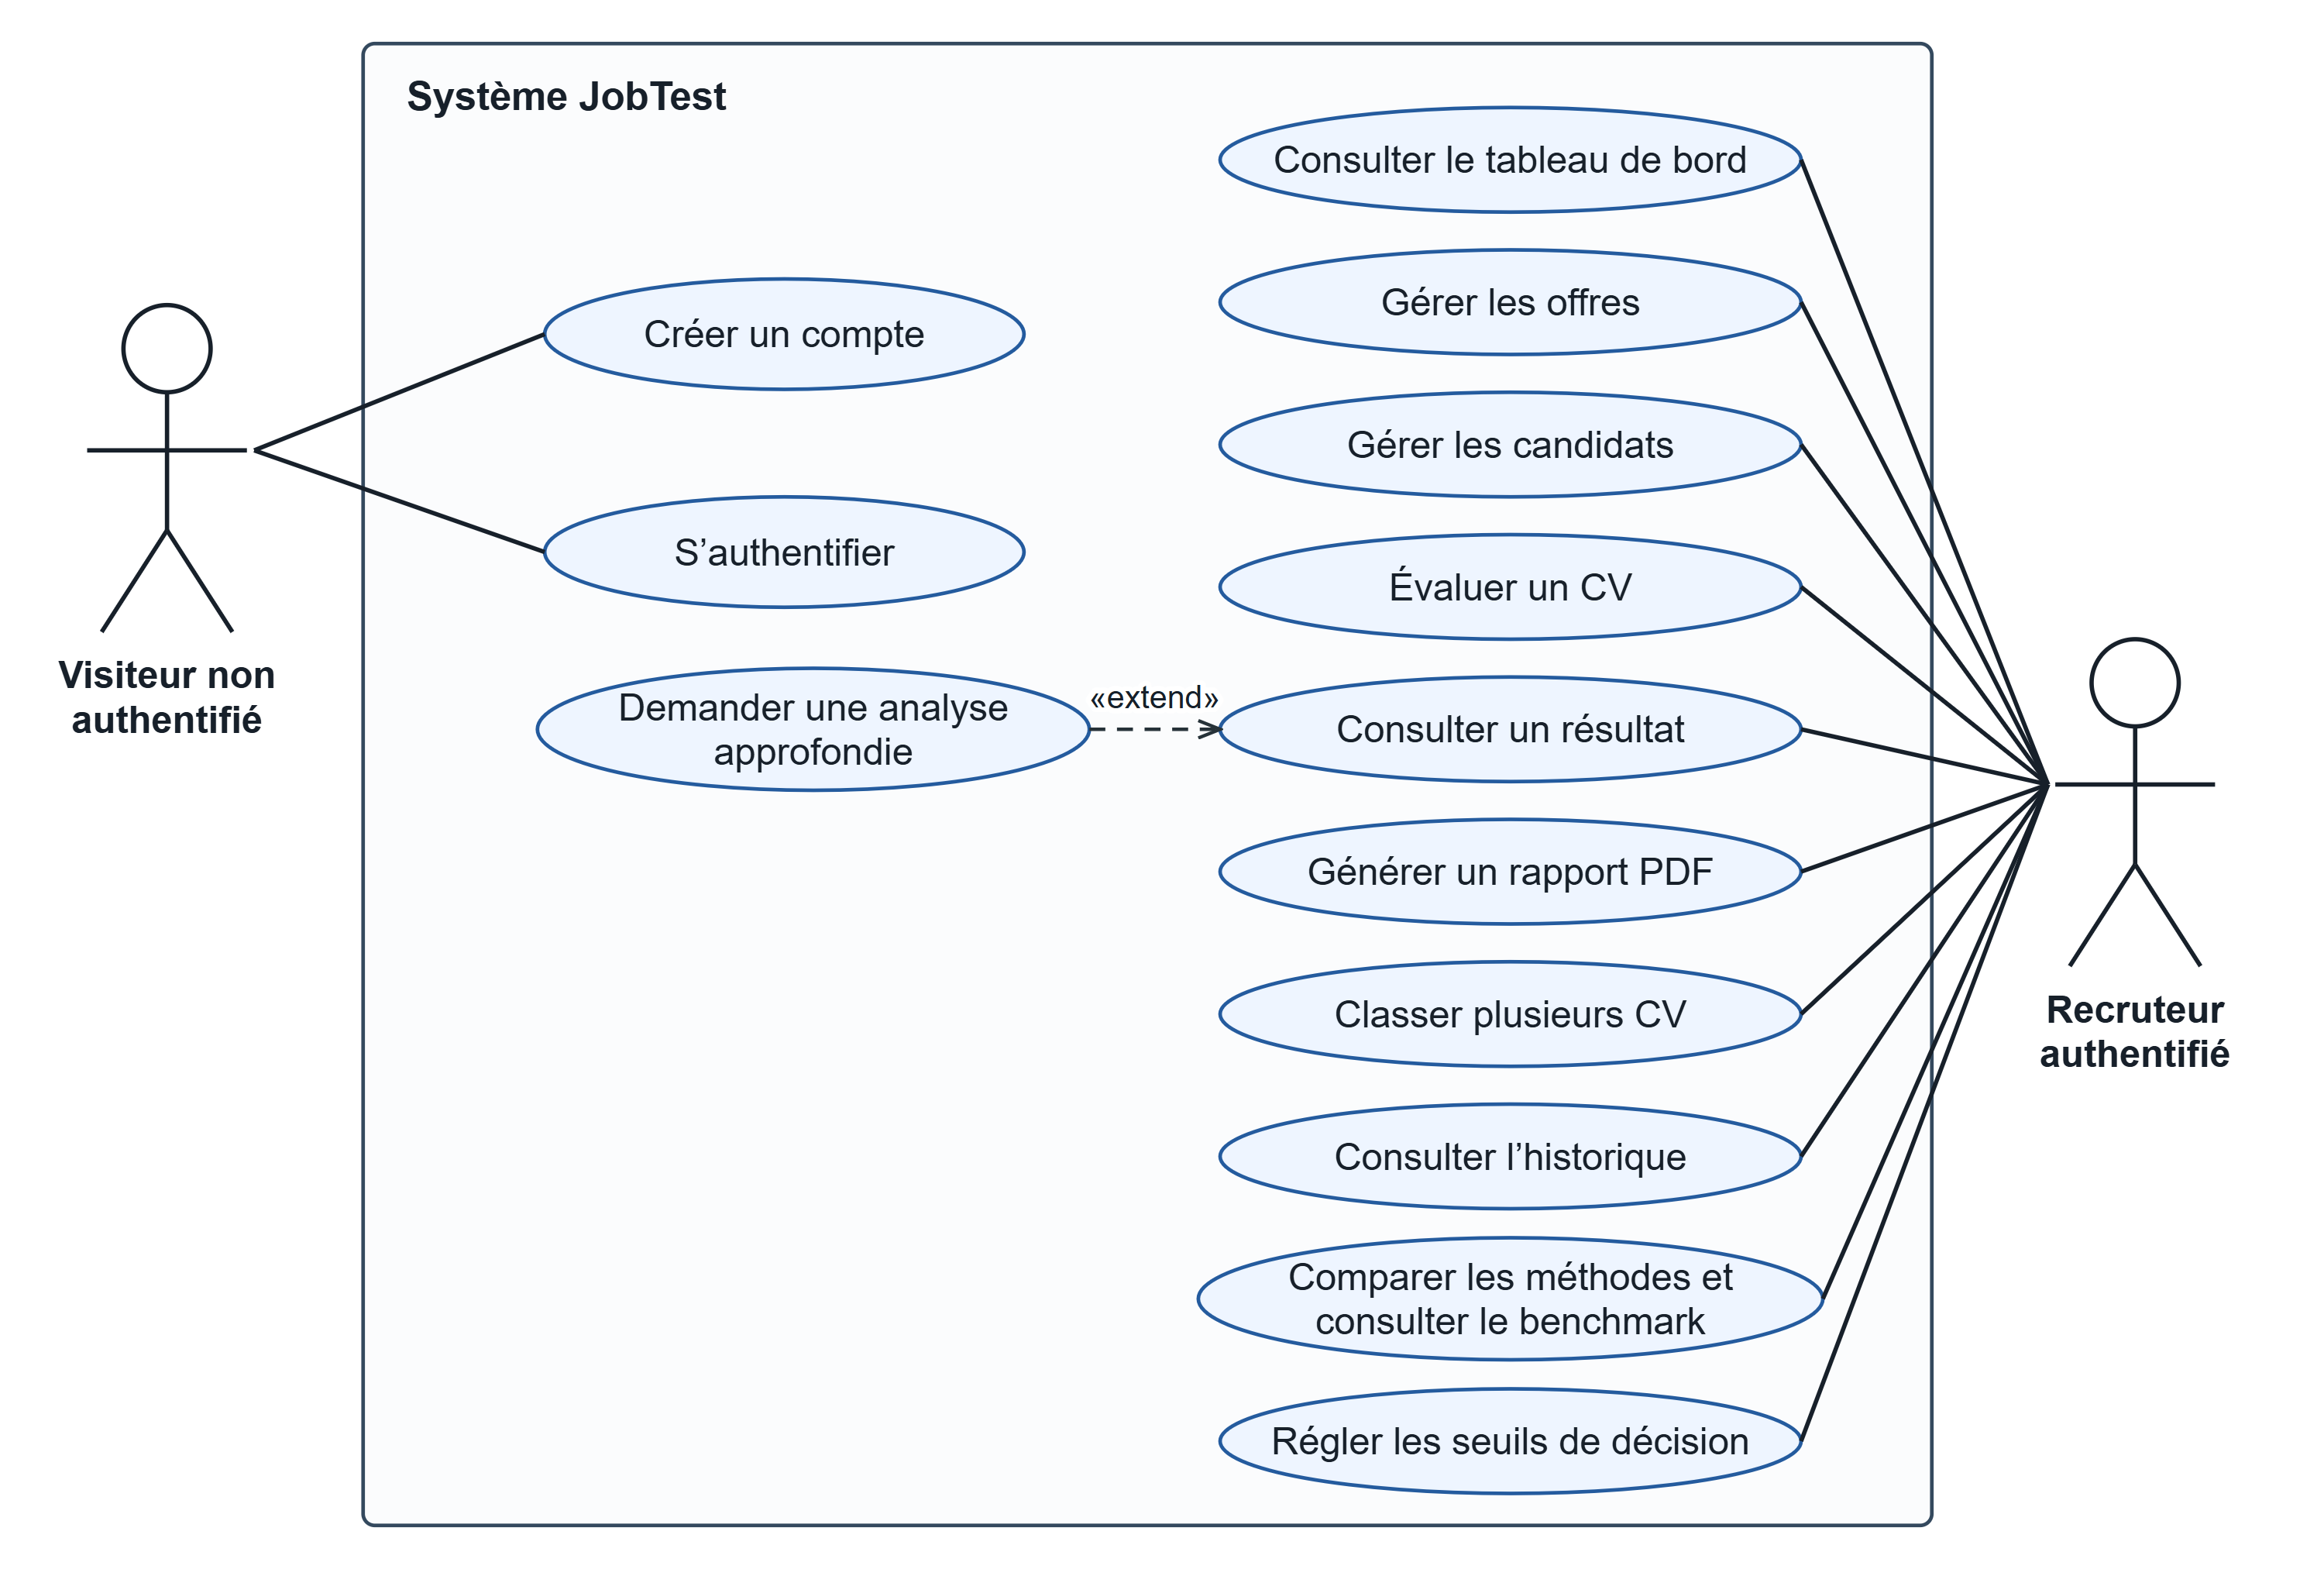
\includegraphics[width=.95\textwidth,height=.76\textheight,keepaspectratio]{img/jobtest_use_cases/01_global.png}
\caption{Diagramme global des cas d'utilisation de JobTest}
\label{fig:uc-global}
\end{figure}

Le visiteur reste limité à la création de compte et à l'authentification. Le recruteur porte tous les cas opérationnels. L'analyse approfondie est une extension facultative de la consultation du résultat ; l'export PDF dépend de l'existence d'un résultat. L'authentification est une précondition aux autres cas et non un lien \textit{include} répété dans tout le diagramme.

\section{Raffinement des cas d'utilisation principaux}
Les diagrammes suivants détaillent les huit parcours significatifs sans transformer les opérations internes en cas d'utilisation. Les relations \textit{include} expriment une sous-action nécessaire au but représenté ; la relation \textit{extend} est réservée à l'analyse approfondie facultative.

La série s'ouvre avec la figure~\ref{fig:uc-auth}, consacrée à l'authentification et à la gestion de session.

\begin{figure}[htbp]\centering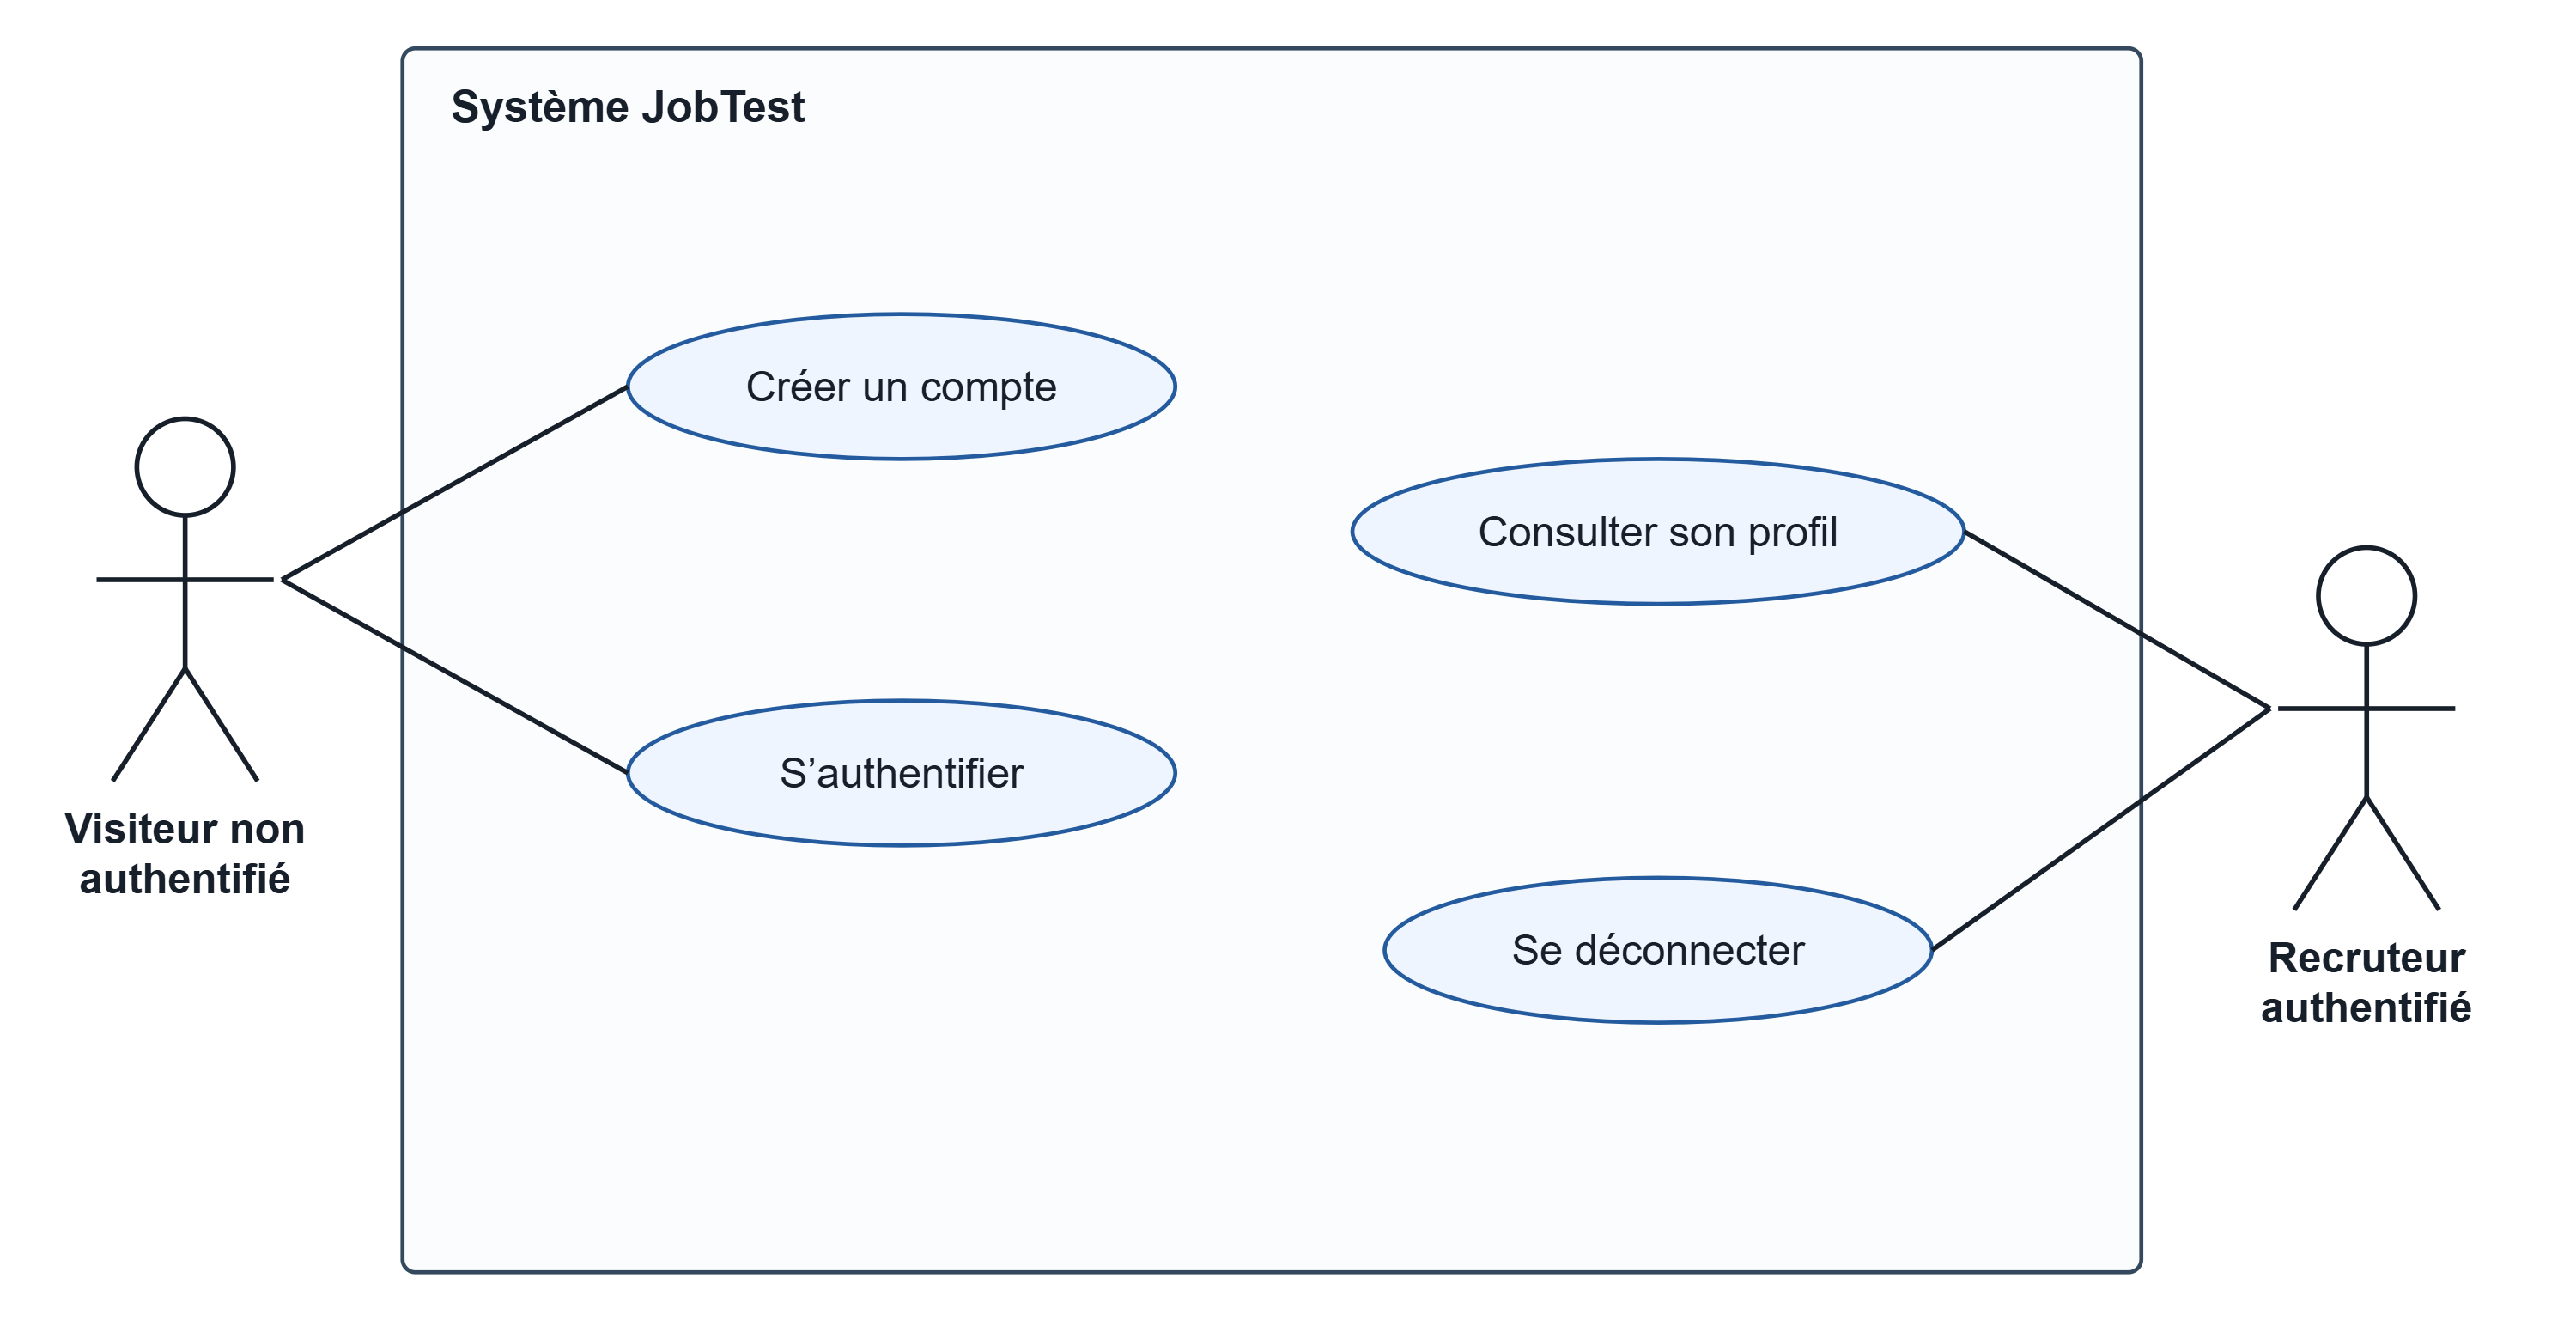
\includegraphics[width=.95\textwidth,height=.76\textheight,keepaspectratio]{img/jobtest_use_cases/02_authentification.png}\caption{UC-01 : authentification et session}\label{fig:uc-auth}\end{figure}
\begin{figure}[htbp]\centering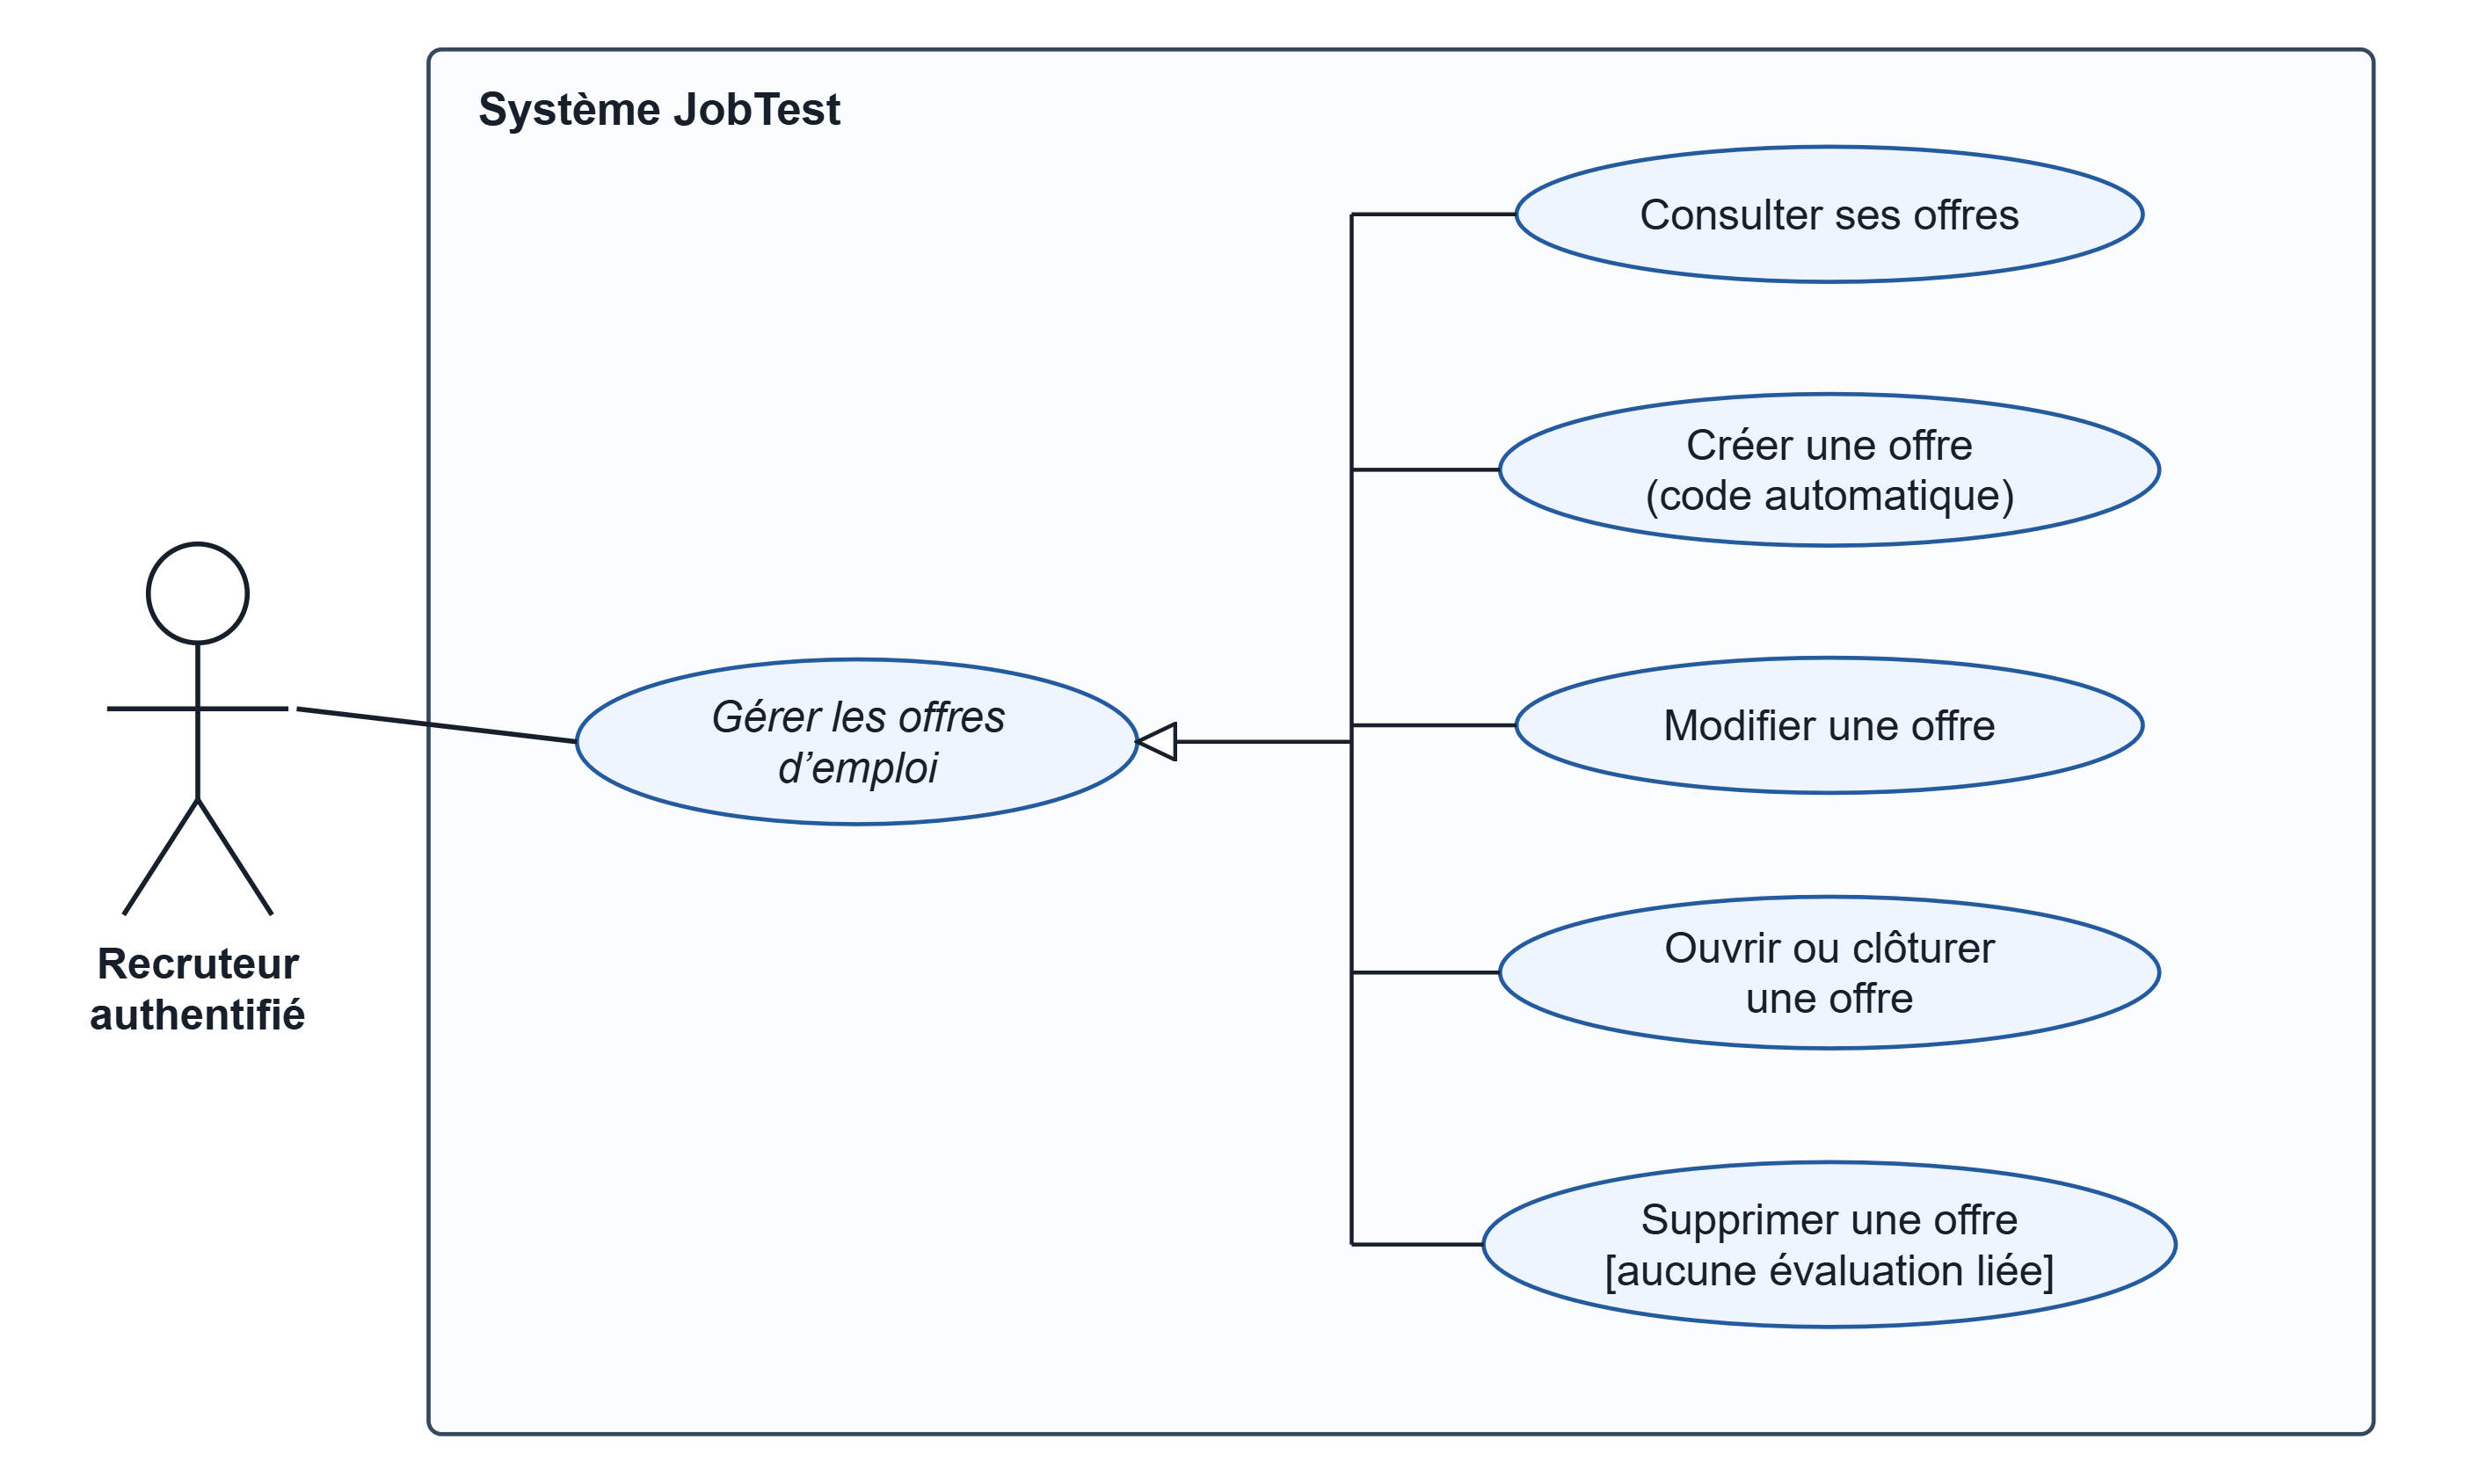
\includegraphics[width=.95\textwidth,height=.76\textheight,keepaspectratio]{img/jobtest_use_cases/03_offres.png}\caption{UC-02 : gestion des offres d'emploi}\label{fig:uc-jobs}\end{figure}
\begin{figure}[htbp]\centering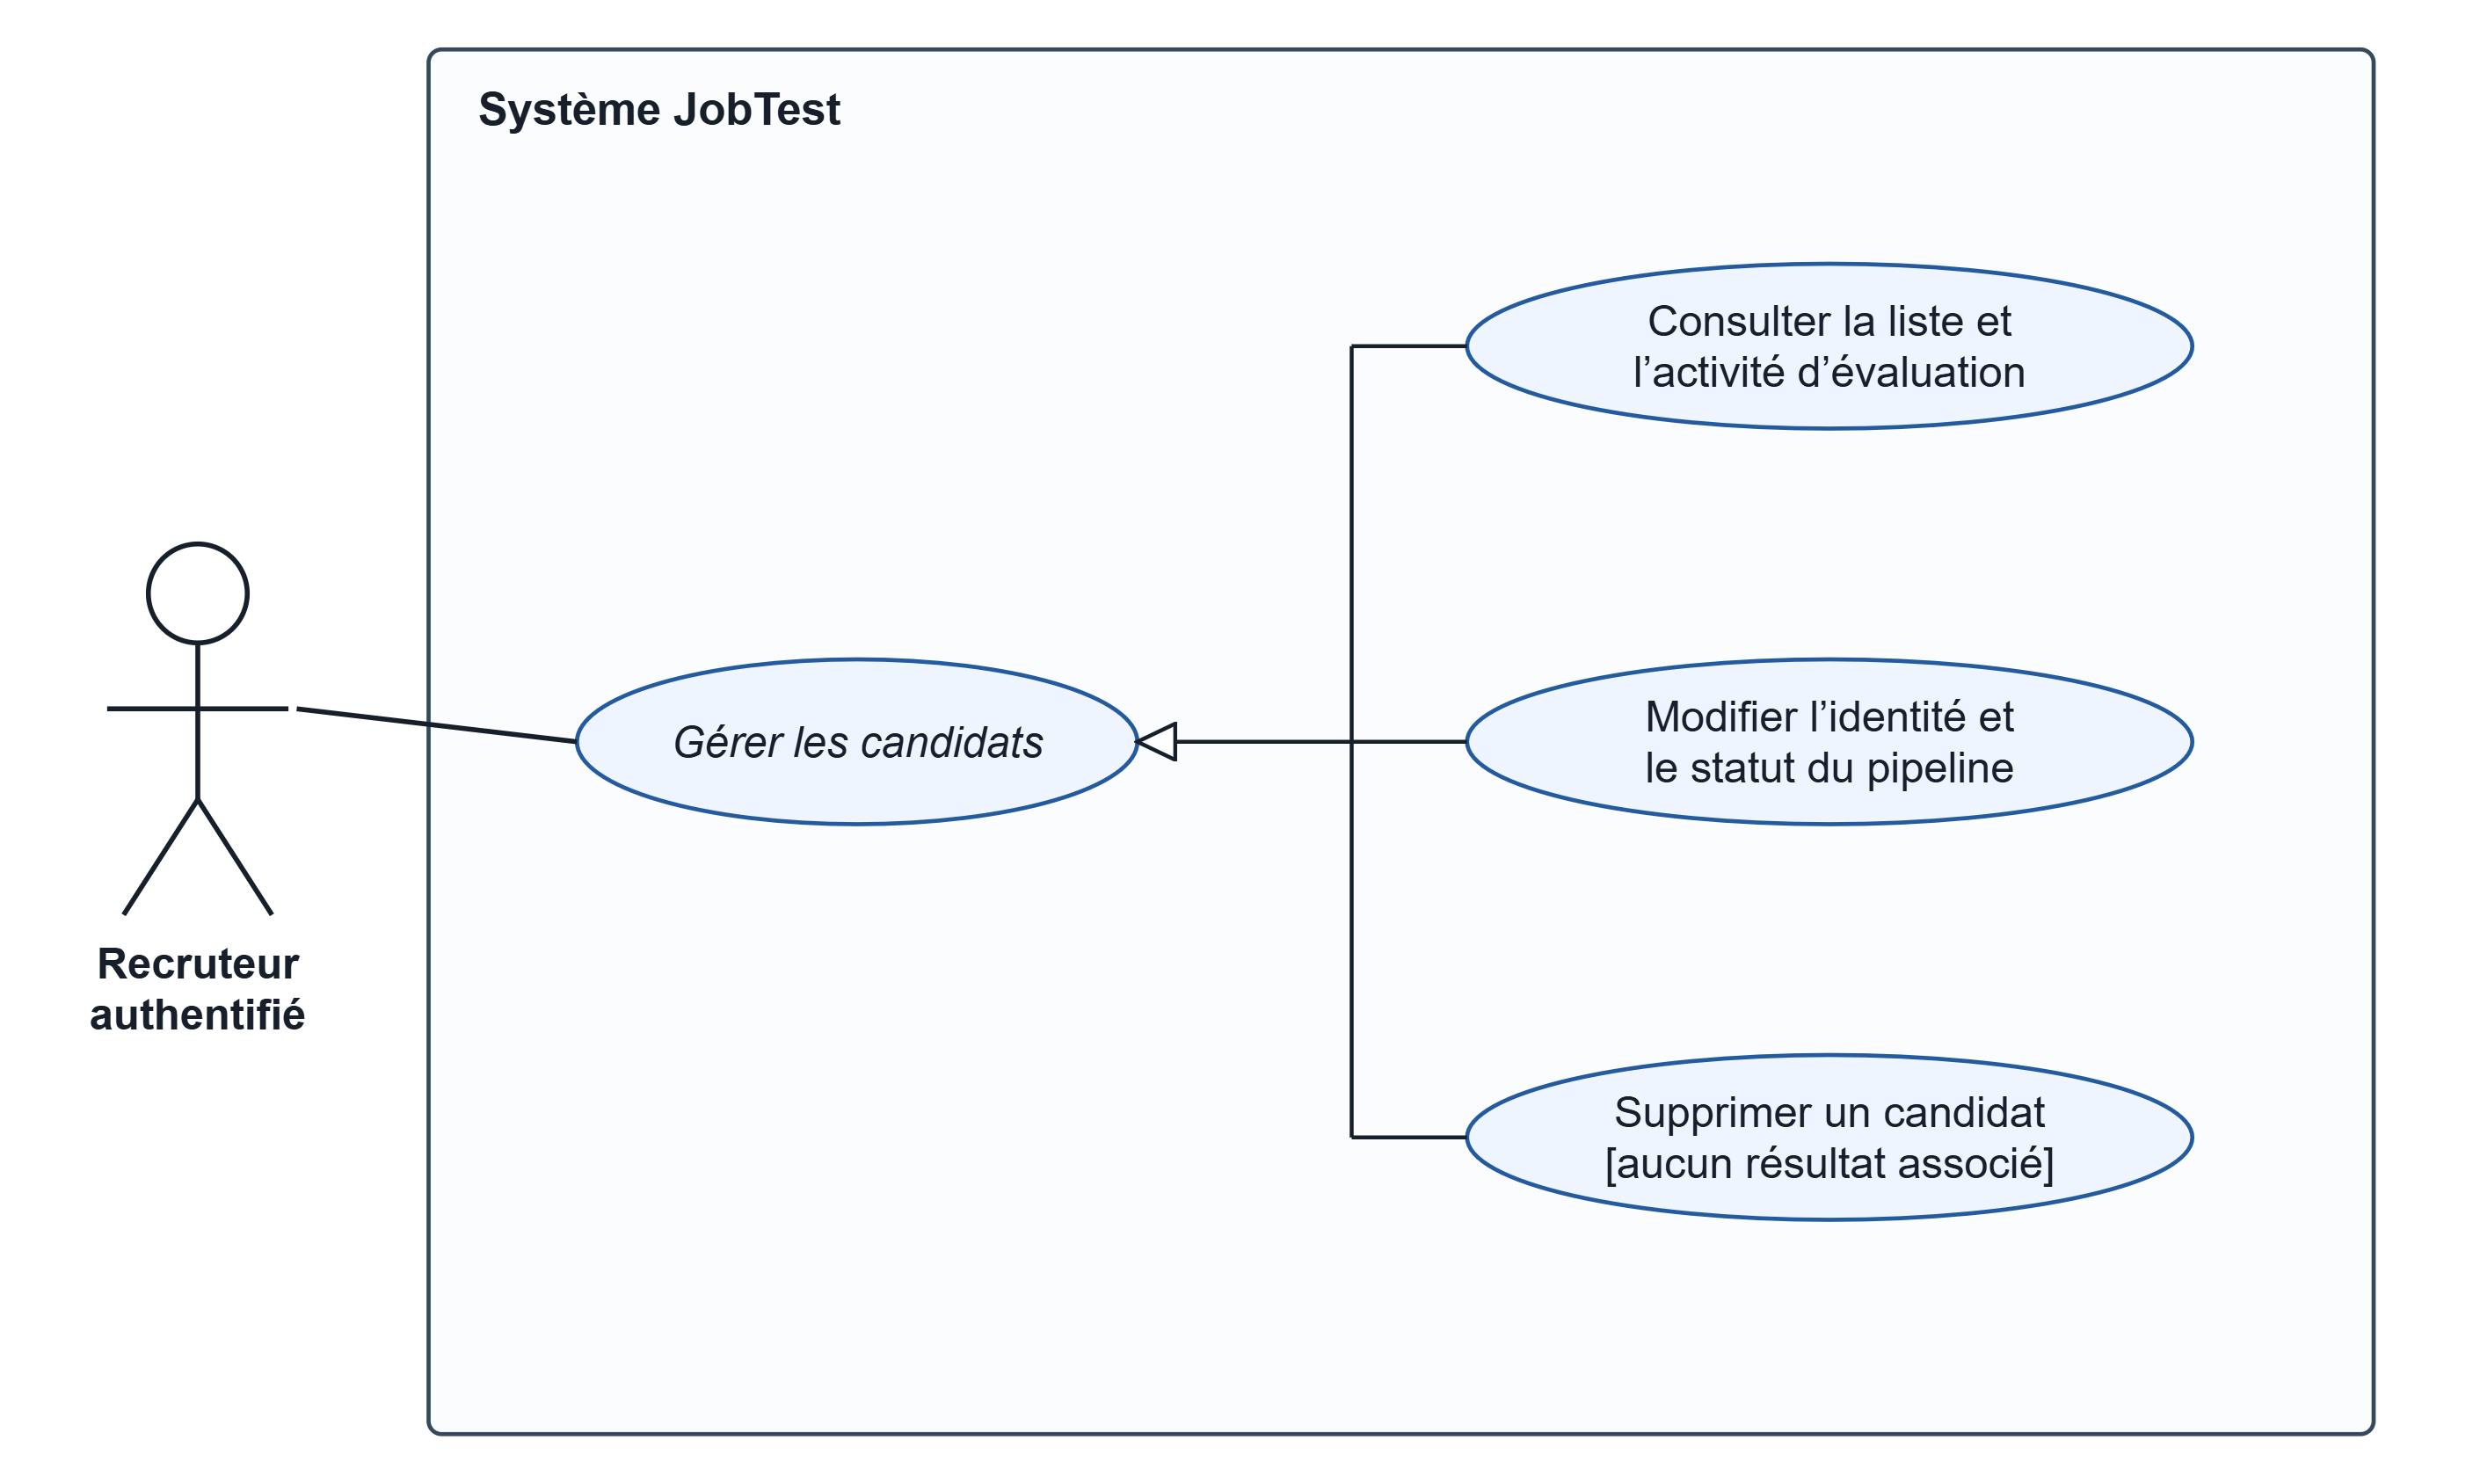
\includegraphics[width=.95\textwidth,height=.76\textheight,keepaspectratio]{img/jobtest_use_cases/04_candidats.png}\caption{UC-03 : gestion des candidats}\label{fig:uc-candidates}\end{figure}
\begin{figure}[htbp]\centering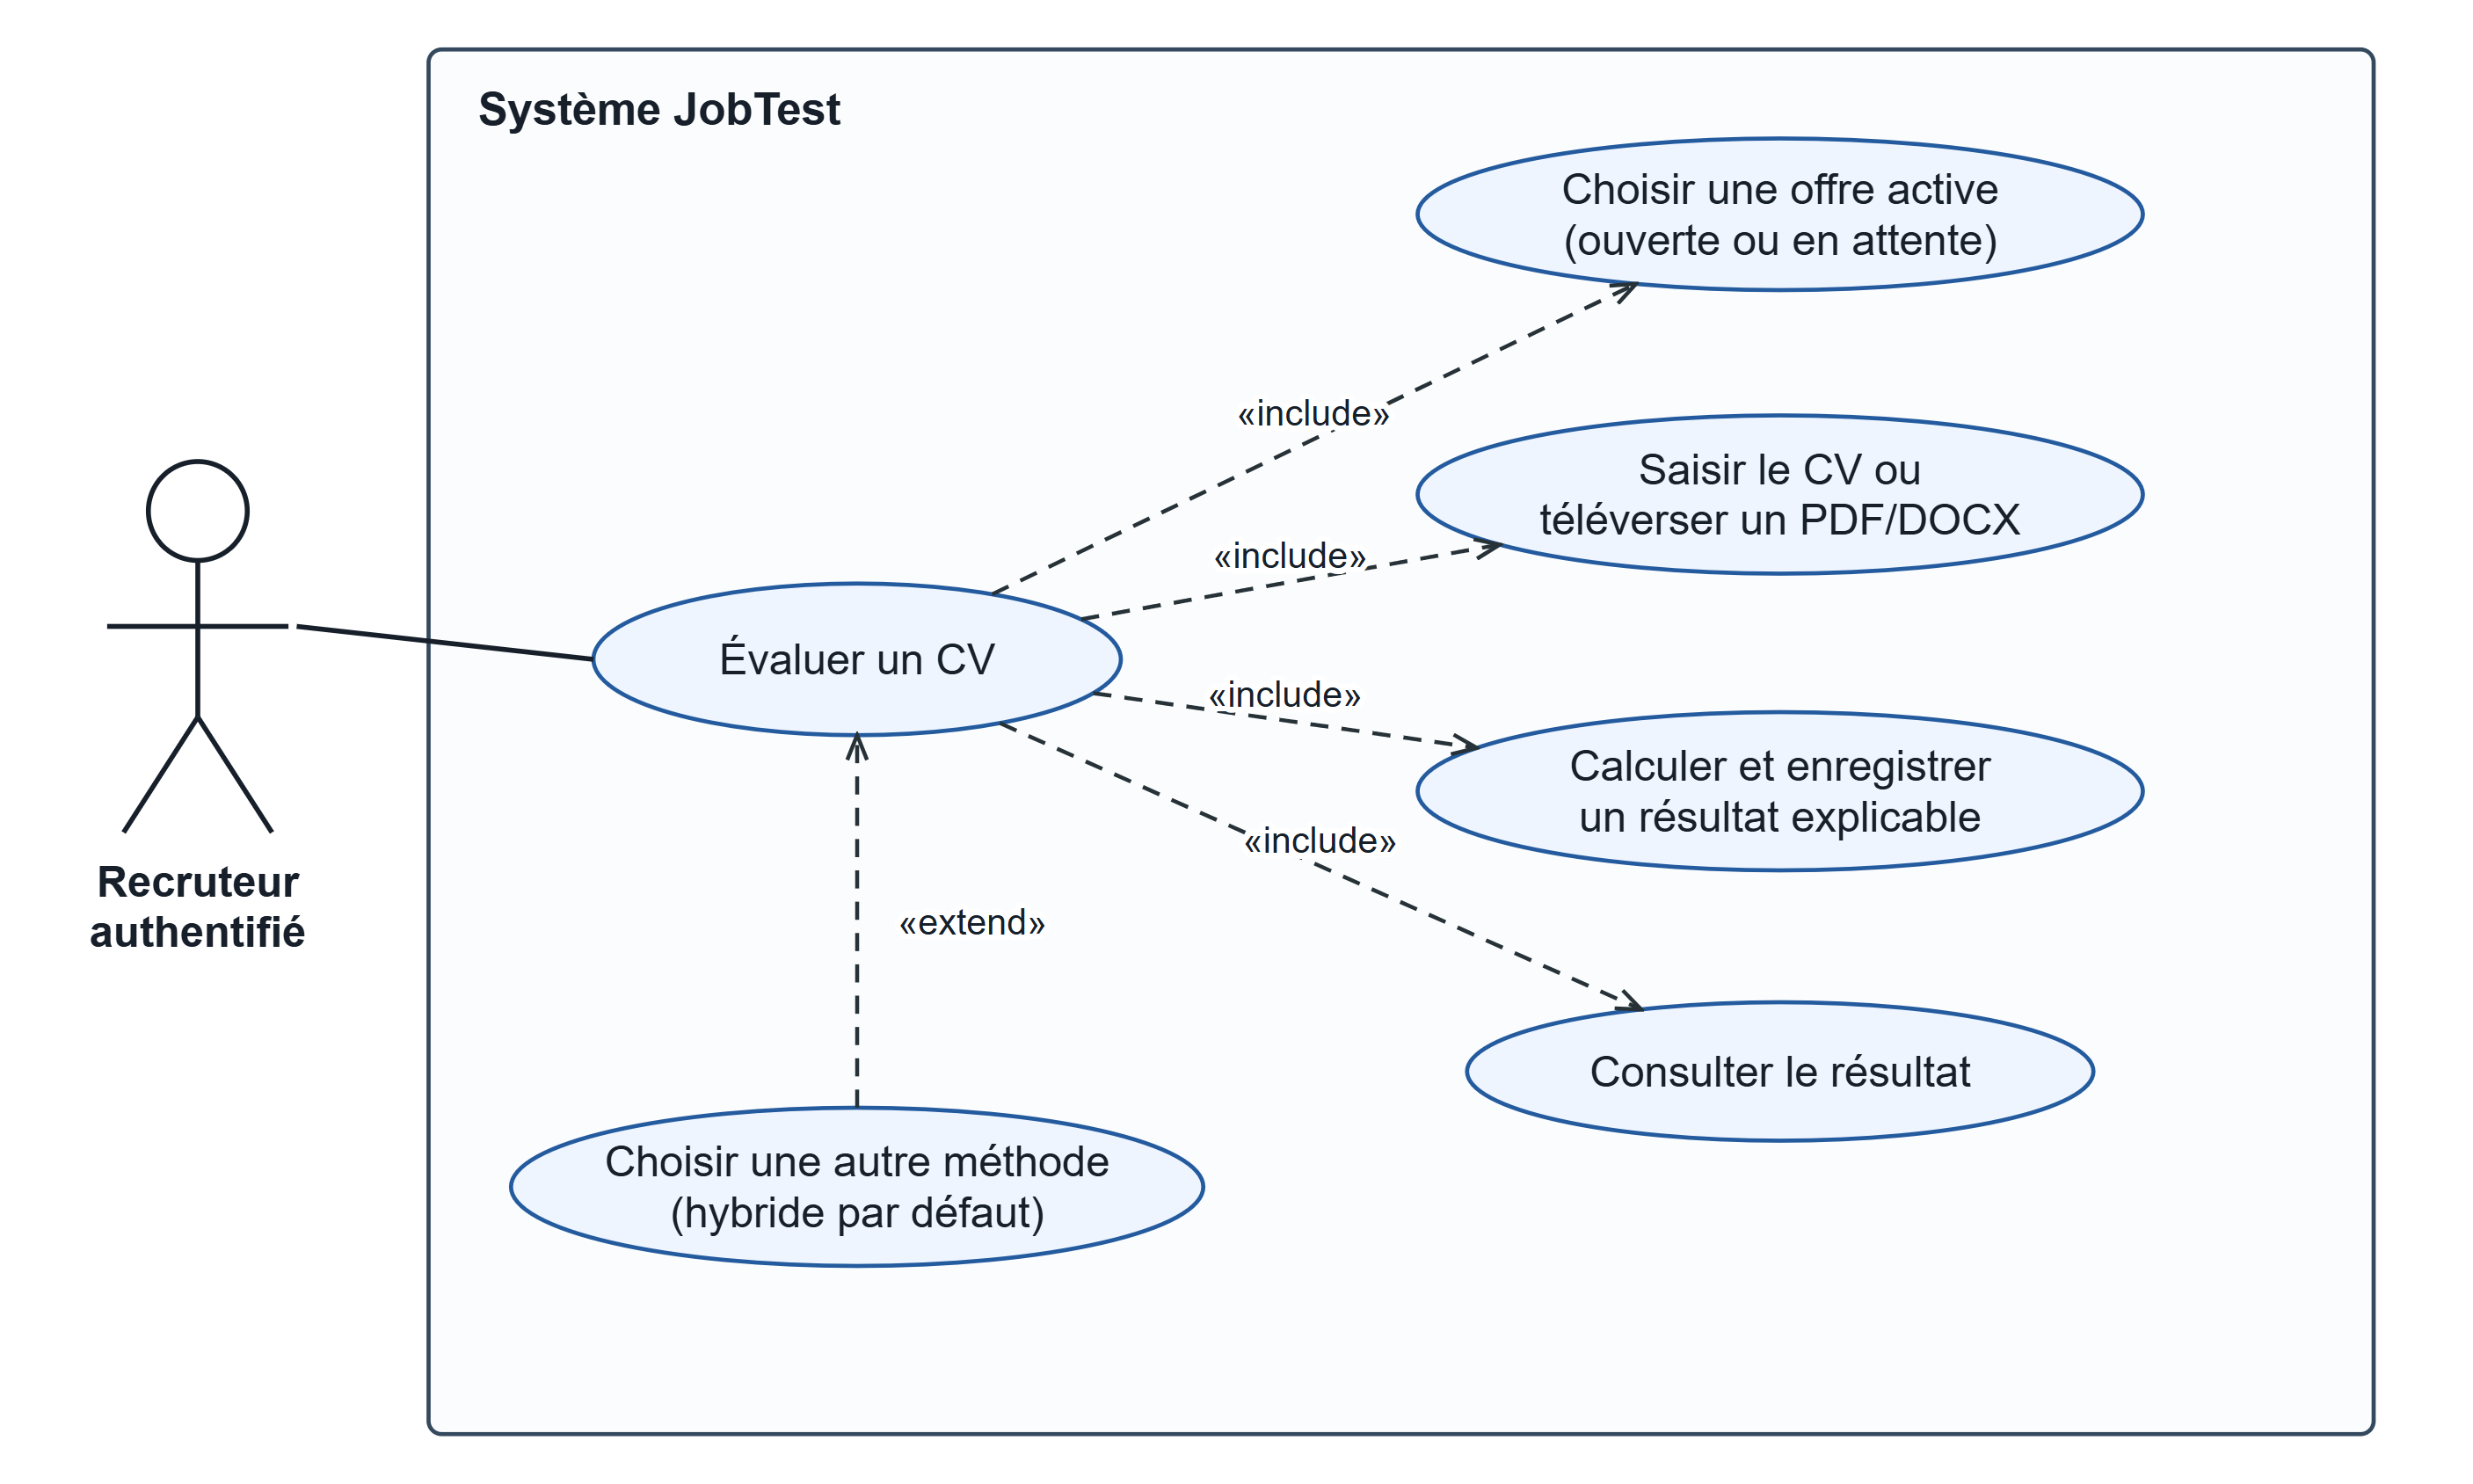
\includegraphics[width=.95\textwidth,height=.76\textheight,keepaspectratio]{img/jobtest_use_cases/05_evaluation_cv.png}\caption{UC-04 : évaluation d'un CV}\label{fig:uc-evaluation}\end{figure}
\begin{figure}[htbp]\centering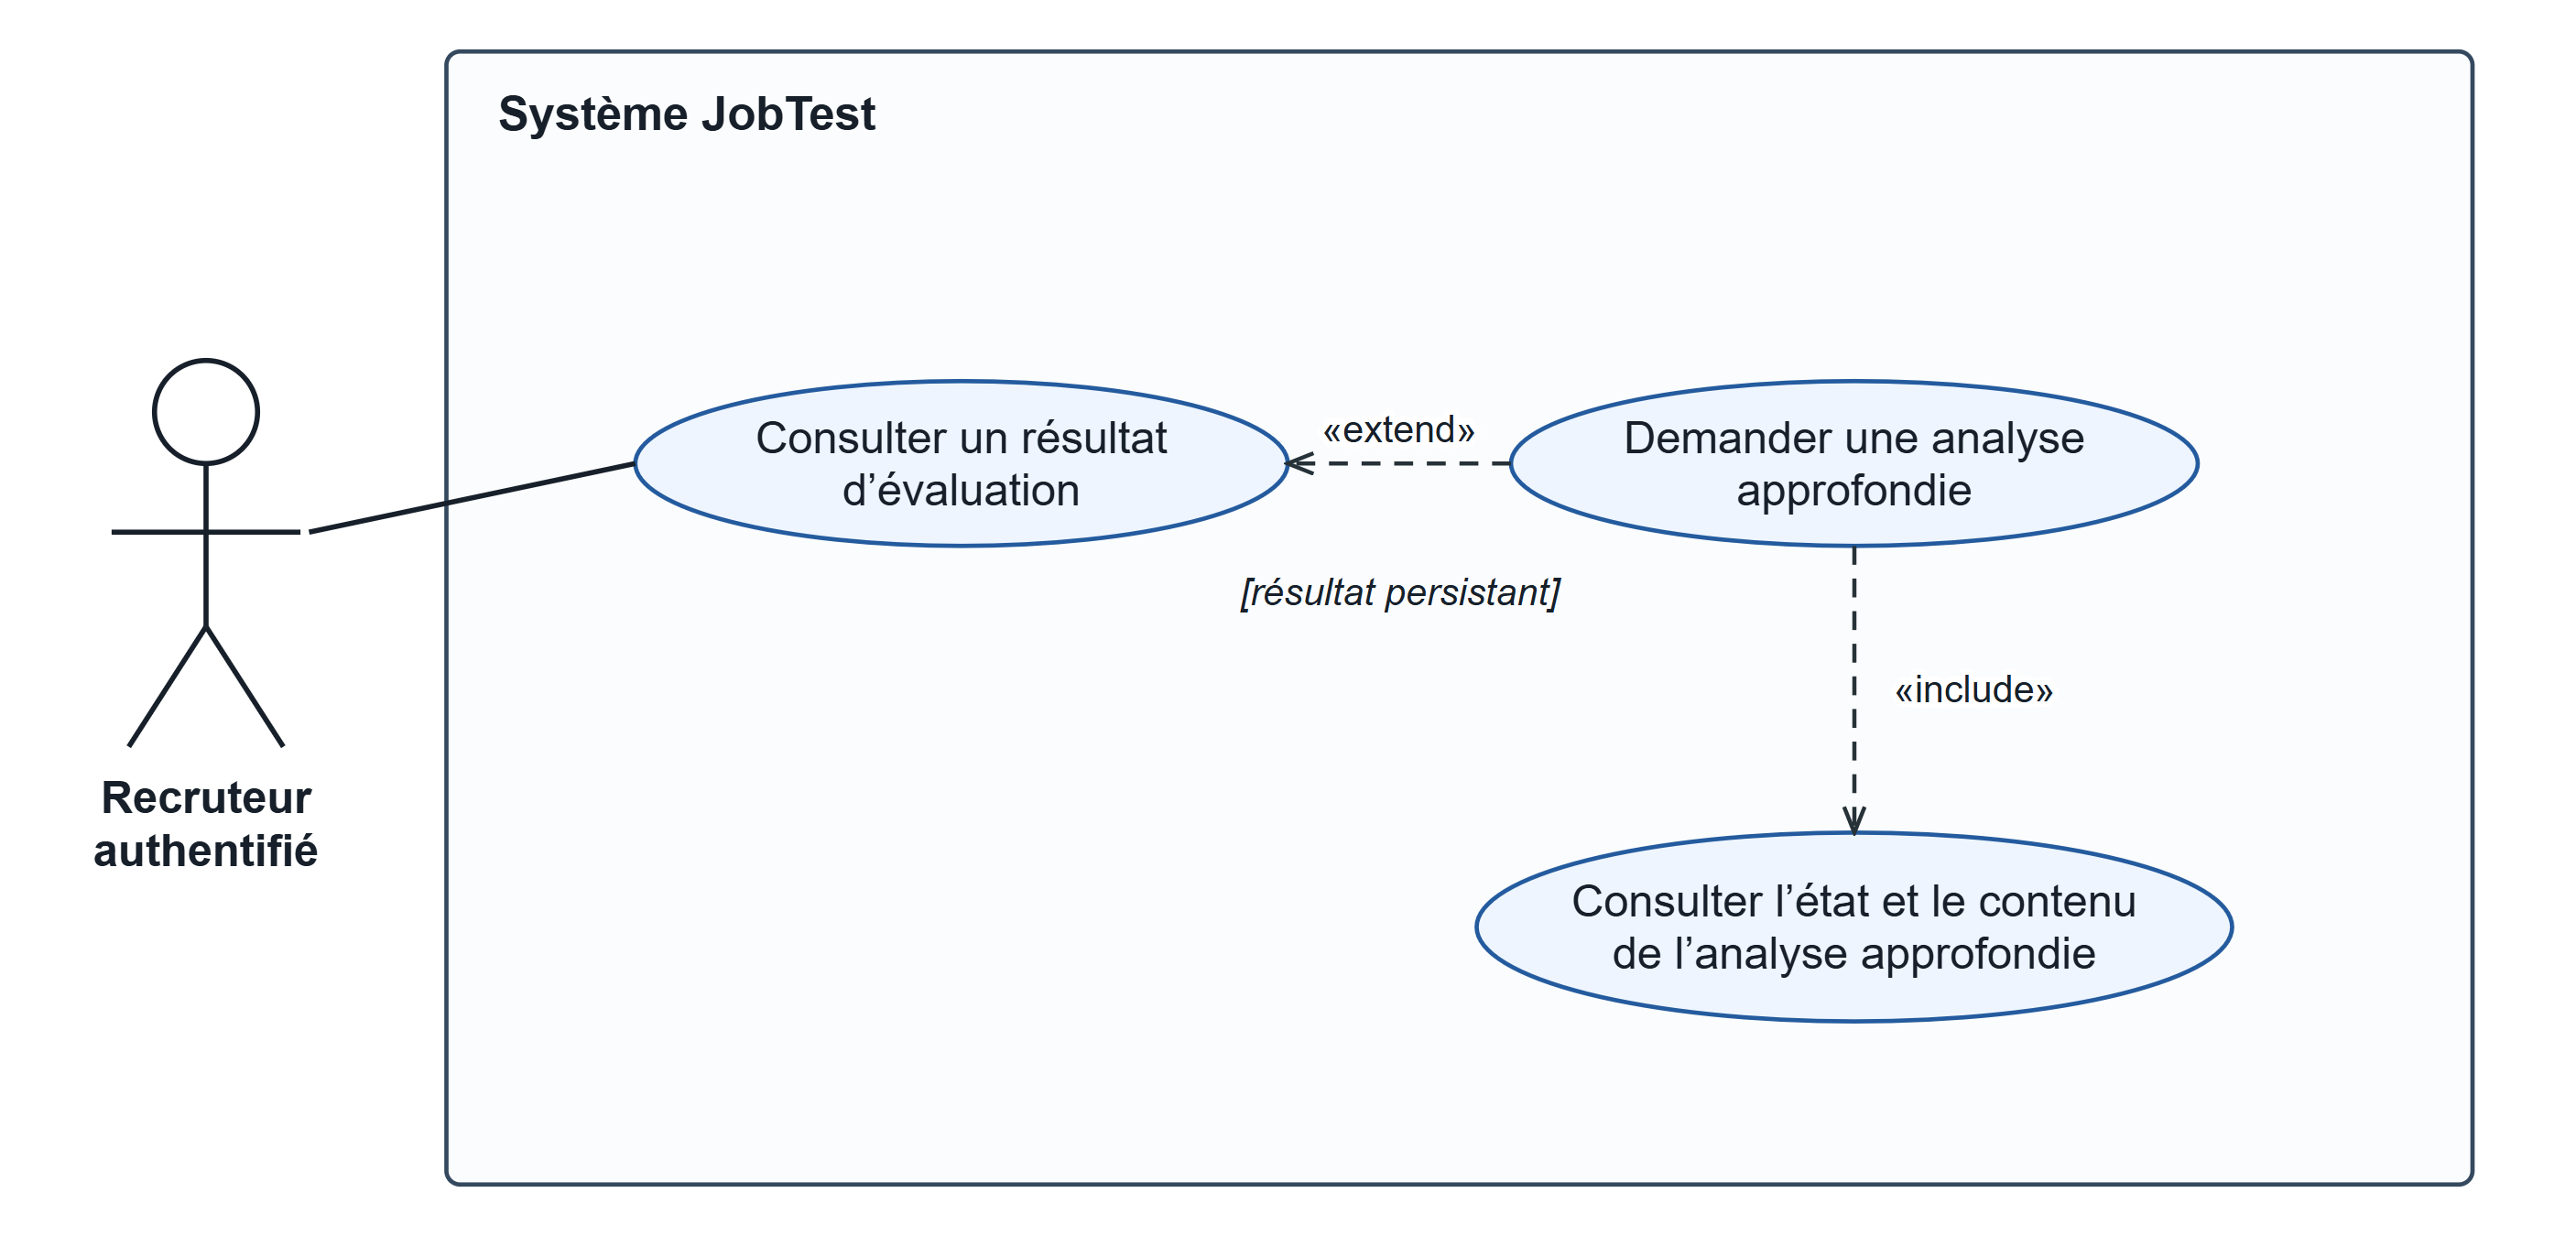
\includegraphics[width=.95\textwidth,height=.76\textheight,keepaspectratio]{img/jobtest_use_cases/06_analyse_approfondie.png}\caption{UC-05 : analyse approfondie optionnelle}\label{fig:uc-deep}\end{figure}
La production du rapport PDF, déclenchée depuis un résultat existant, est représentée par la figure~\ref{fig:uc-report}.

\begin{figure}[htbp]\centering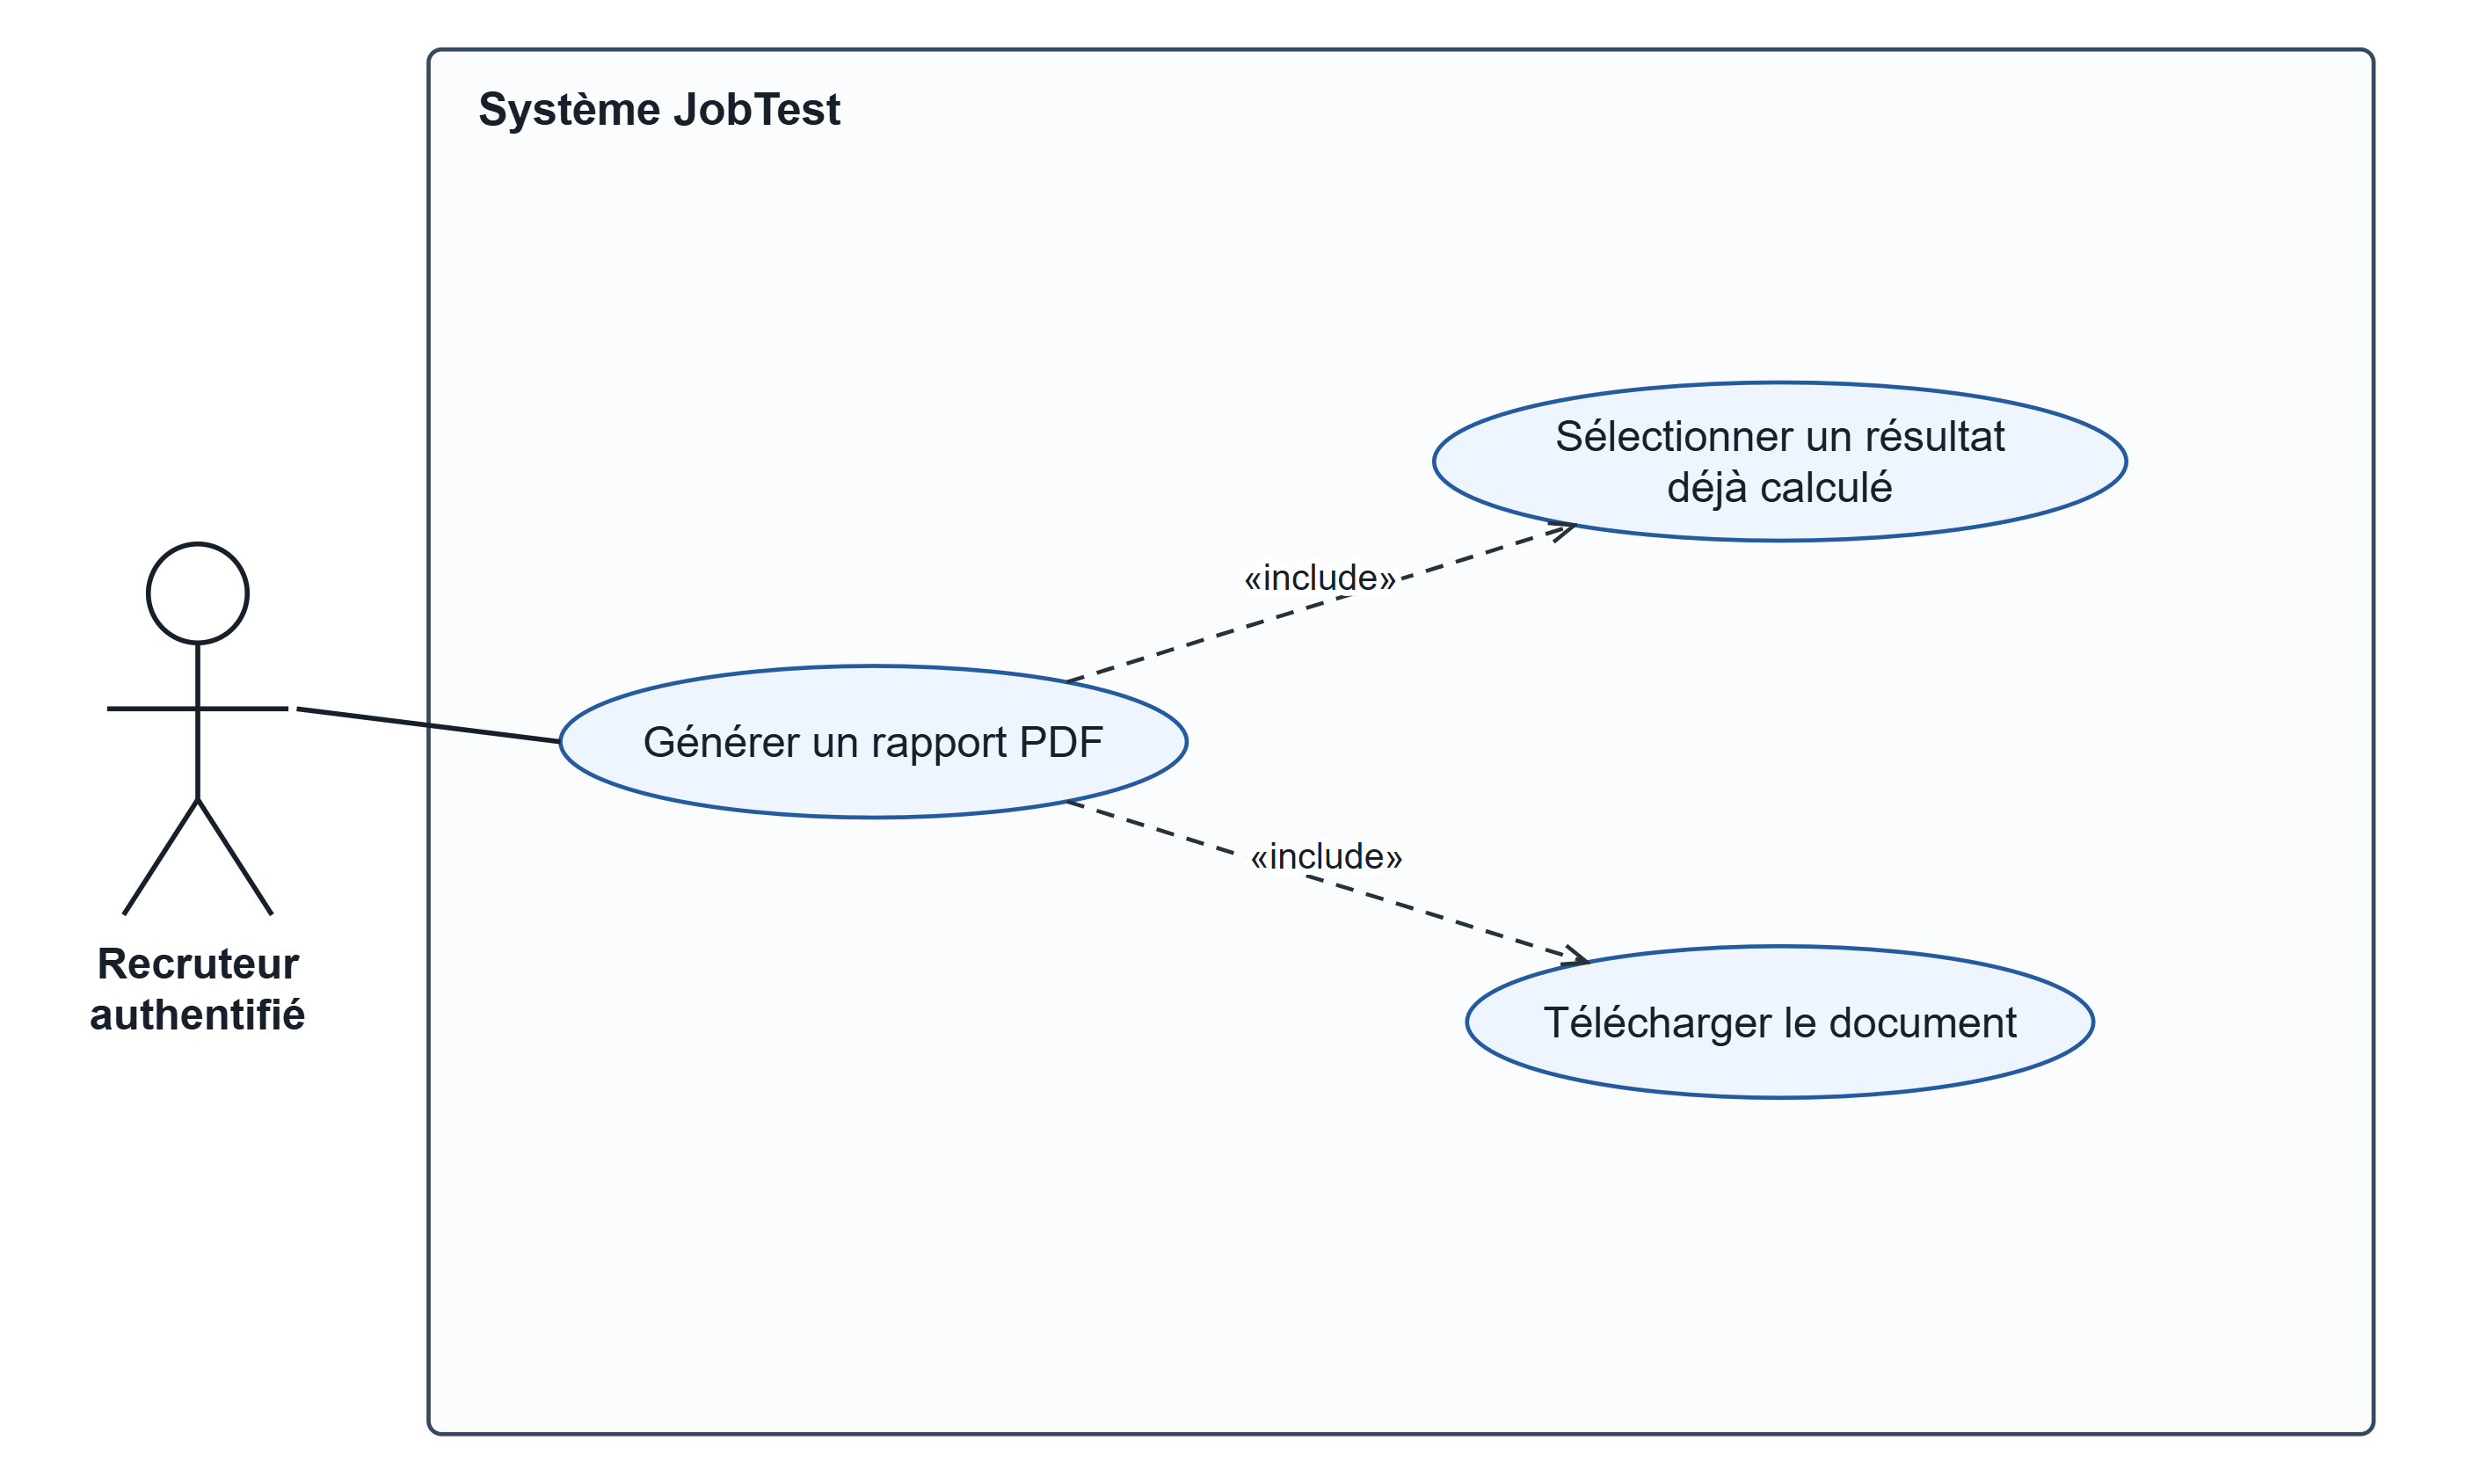
\includegraphics[width=.95\textwidth,height=.76\textheight,keepaspectratio]{img/jobtest_use_cases/07_rapport_pdf.png}\caption{UC-06 : génération du rapport PDF}\label{fig:uc-report}\end{figure}
Le classement de plusieurs candidatures sur une même offre fait l'objet de la figure~\ref{fig:uc-ranking}.

\begin{figure}[htbp]\centering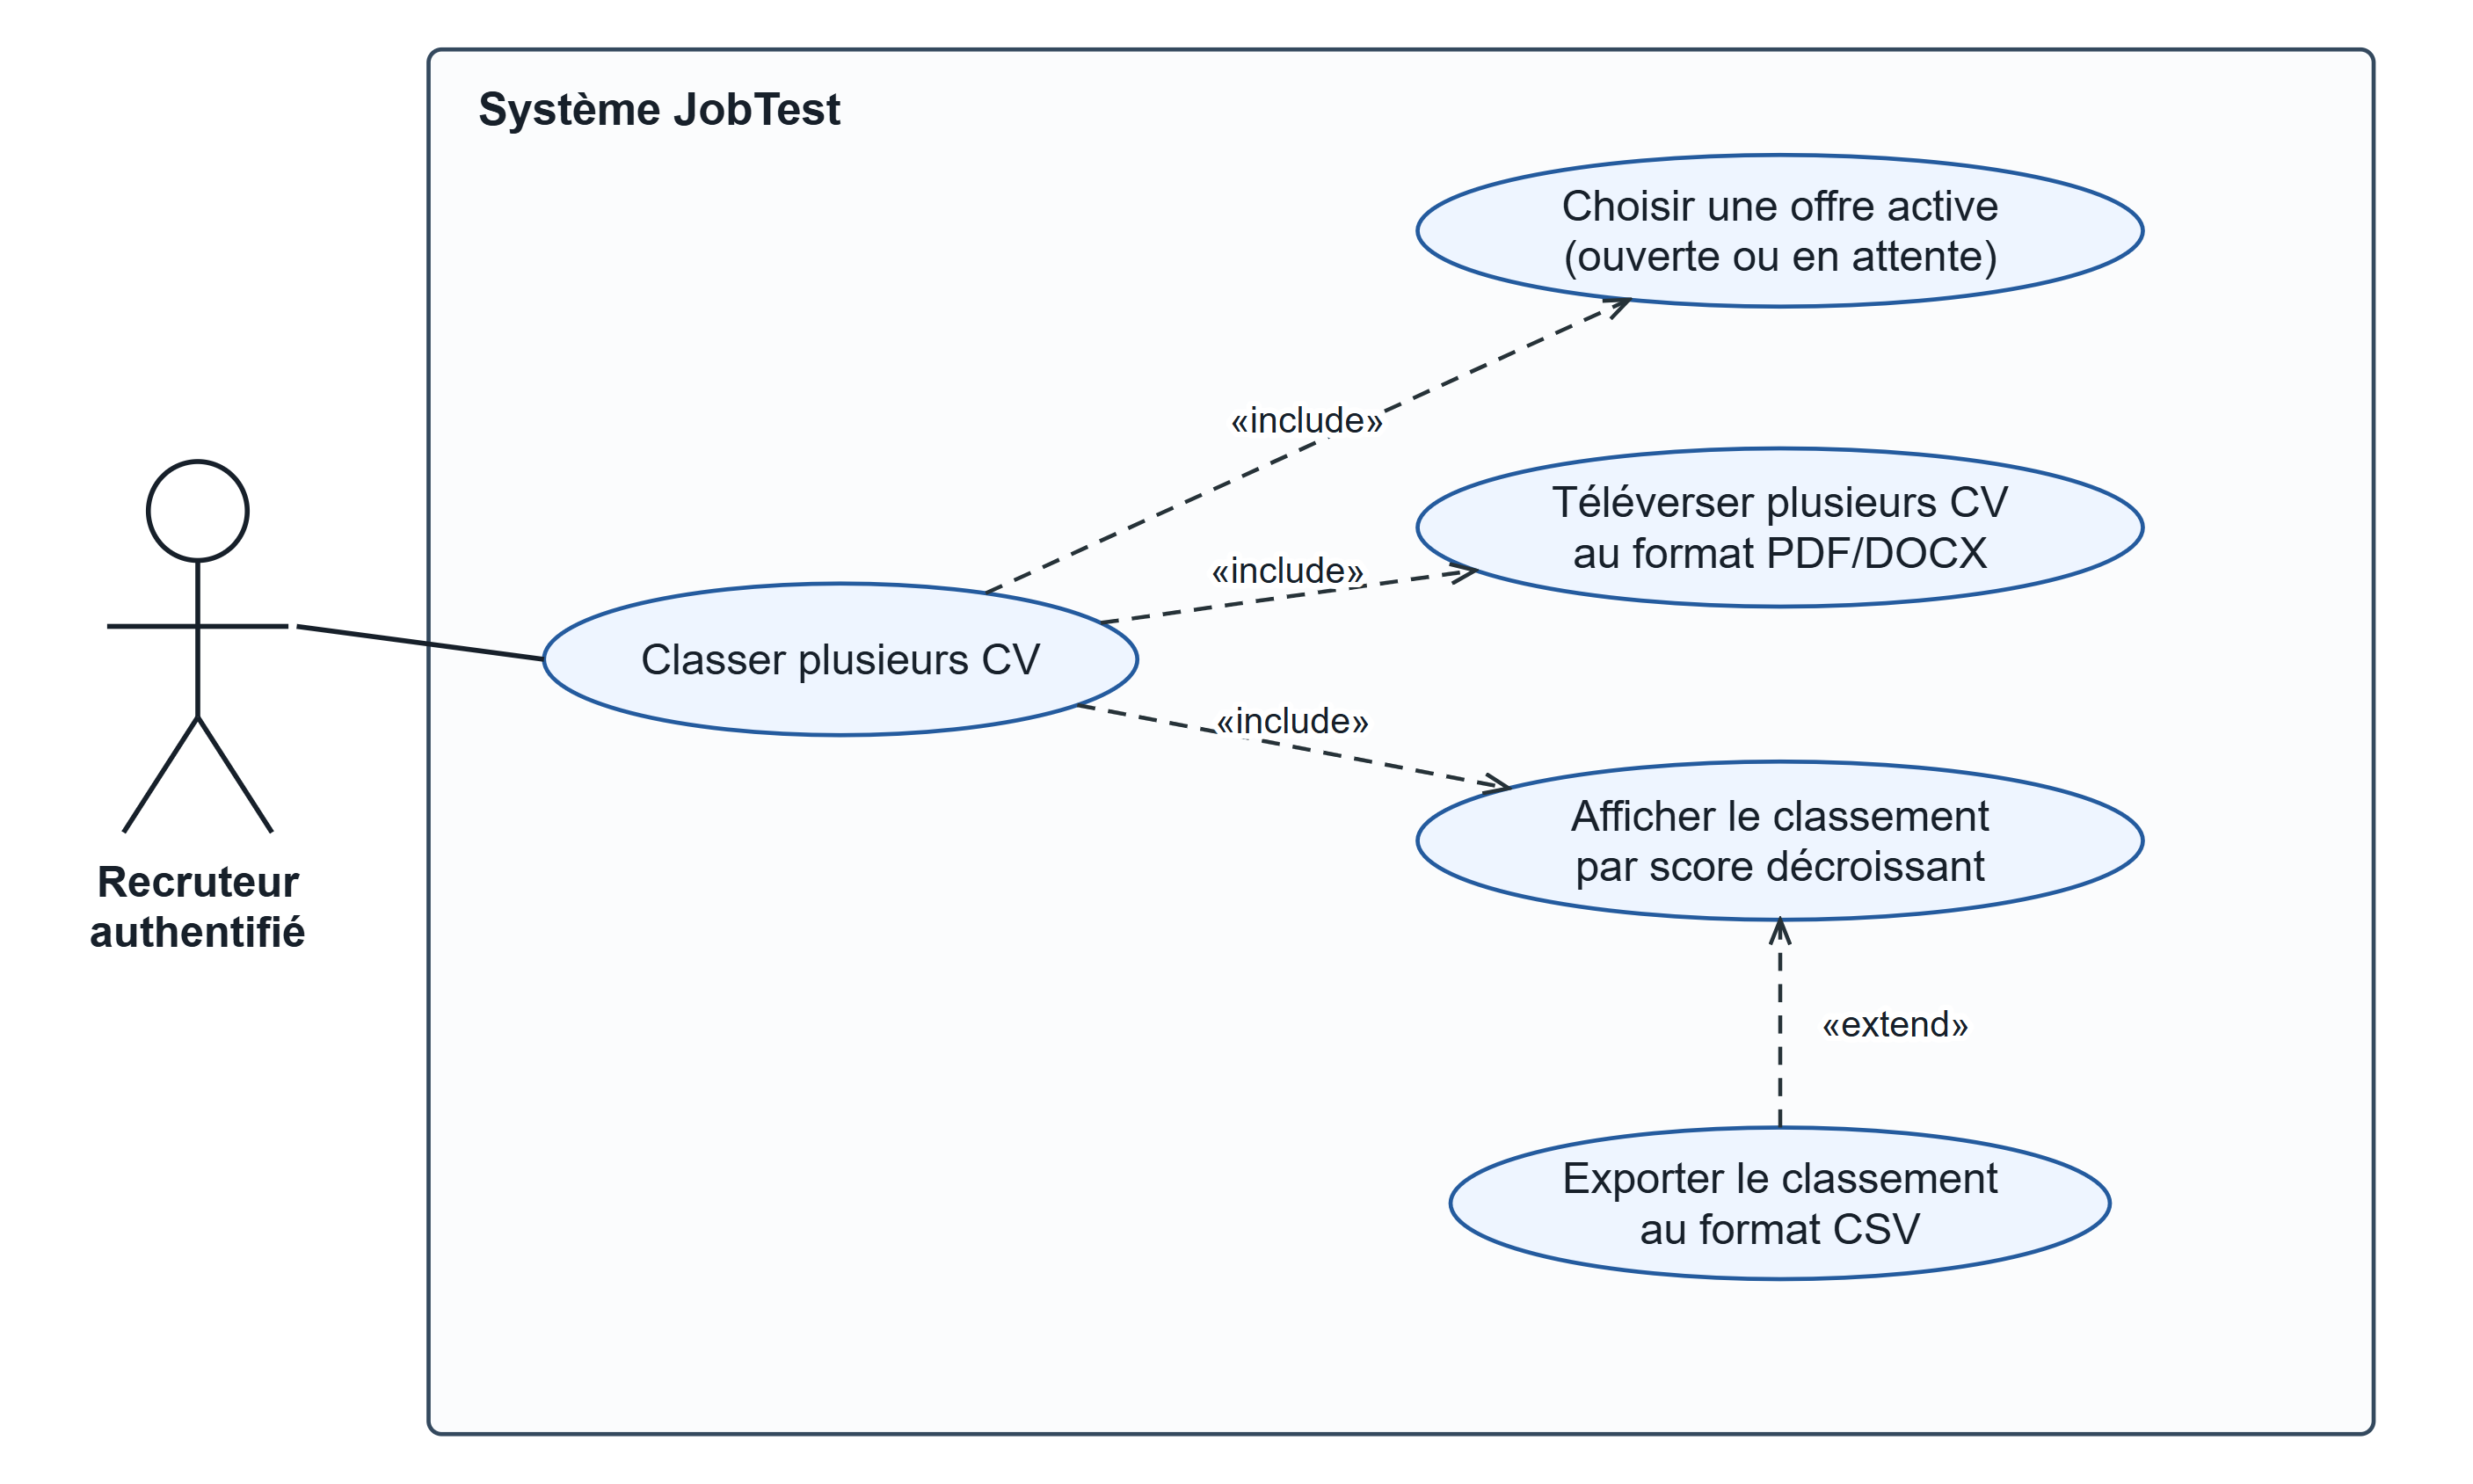
\includegraphics[width=.95\textwidth,height=.76\textheight,keepaspectratio]{img/jobtest_use_cases/08_classement.png}\caption{UC-07 : classement de plusieurs candidats}\label{fig:uc-ranking}\end{figure}
La figure~\ref{fig:uc-history} termine cette série par la consultation de l'historique des évaluations.

\begin{figure}[htbp]\centering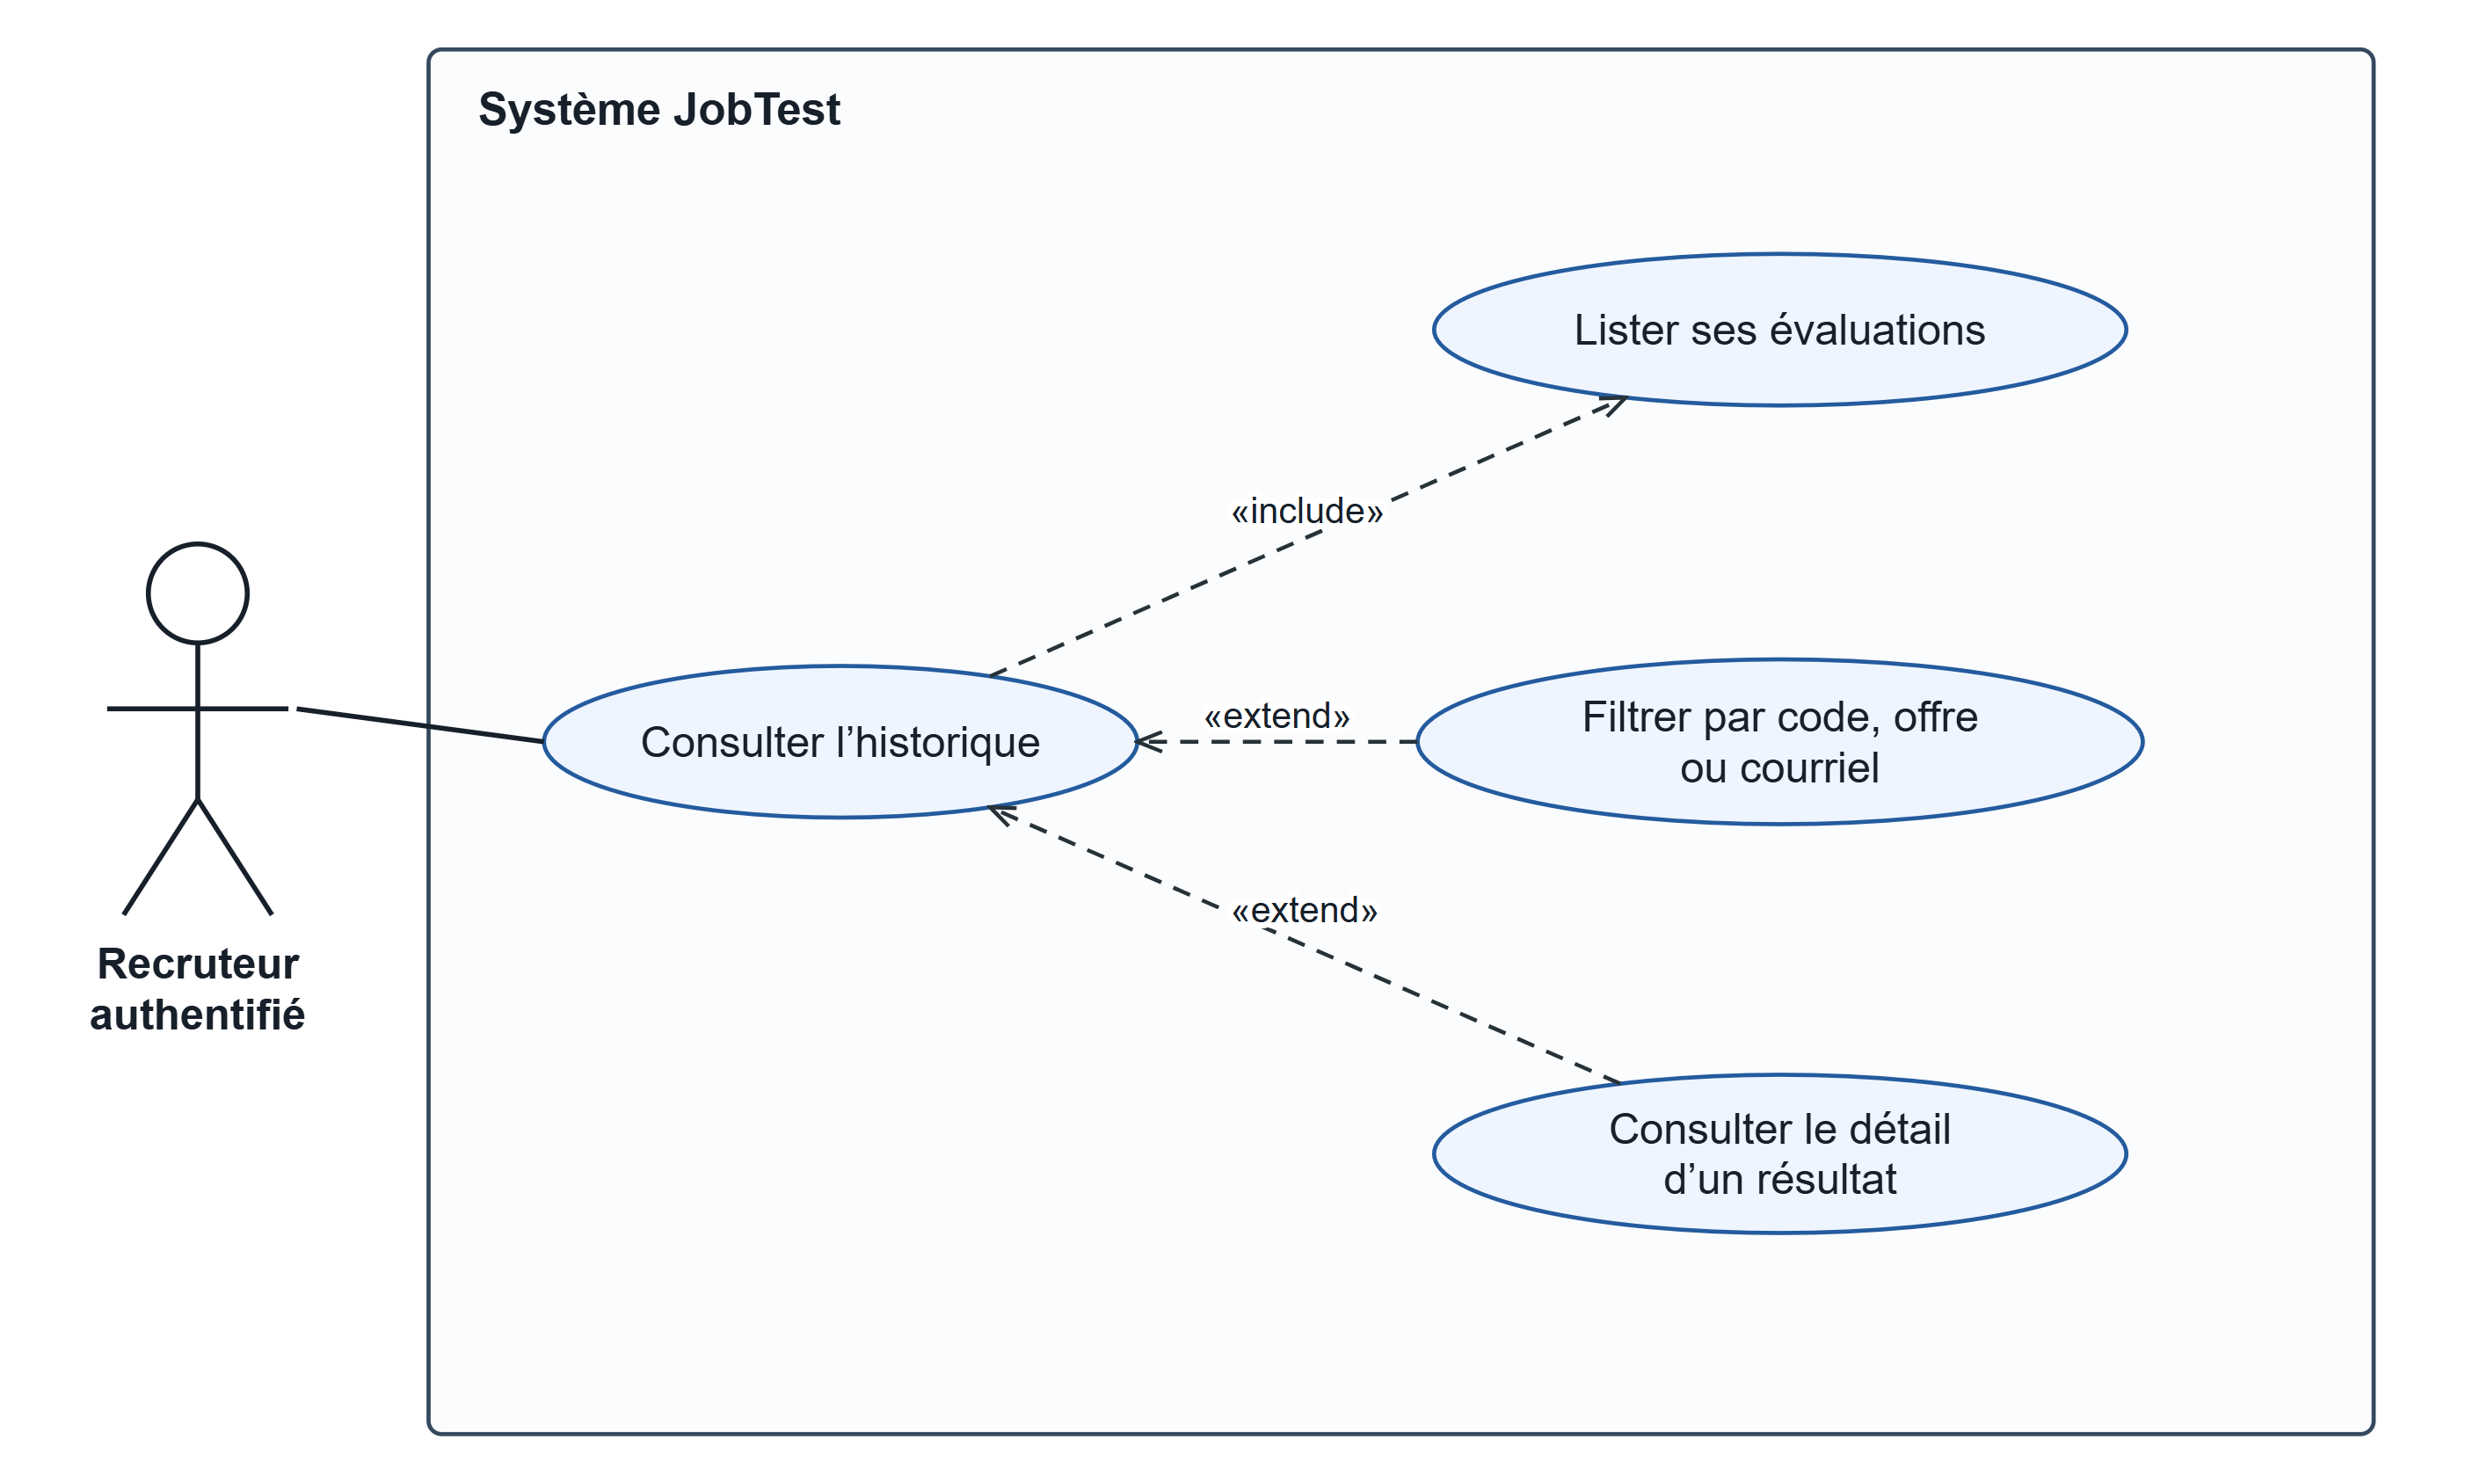
\includegraphics[width=.95\textwidth,height=.76\textheight,keepaspectratio]{img/jobtest_use_cases/09_historique.png}\caption{UC-08 : historique et résultats}\label{fig:uc-history}\end{figure}

Les figures \ref{fig:uc-evaluation} et \ref{fig:uc-deep} isolent explicitement le flux obligatoire d'évaluation du complément LLM. Les figures \ref{fig:uc-jobs} et \ref{fig:uc-candidates} regroupent les opérations CRUD afin de conserver une vue centrée sur le but du recruteur plutôt que sur chaque bouton d'interface.

\clearpage
\section{Descriptions textuelles des cas d'utilisation}
Les huit cas retenus sont maintenant décrits champ par champ, dans le même ordre que les diagrammes précédents. 

Le tableau~\ref{tab:uc01} commence par le cas d'authentification.

\small
\begin{longtable}{|p{3.25cm}|p{11.4cm}|}
\caption{UC-01 : s'authentifier}\label{tab:uc01}\\hline \textbf{Champ} & \textbf{Description}\\hline
Identifiant & UC-01\\ Titre & S'authentifier\\ Acteur principal & Visiteur non authentifié\\ Objectif & Ouvrir une session recruteur donnant accès aux données possédées.\\ Déclencheur & Le visiteur valide le formulaire de connexion.\\ Préconditions & Un compte recruteur existe.\\ Postconditions & Le JWT est stocké côté client et le profil courant est récupérable.\\ Scénario nominal & 1. Le visiteur saisit e-mail et mot de passe. 2. Le système vérifie les identifiants. 3. Le système émet le JWT bearer. 4. L'interface charge \texttt{/auth/me} puis redirige vers l'espace opérationnel.\\ Scénarios alternatifs & Un nouveau visiteur choisit la création de compte, puis revient à la connexion.\\ Exceptions & Identifiants invalides, compte absent ou API indisponible : message d'erreur, aucune session créée.\\ Règles associées & RG-01.\\hline
\end{longtable}

La gestion des offres est décrite dans le tableau~\ref{tab:uc02}.

\begin{longtable}{|p{3.25cm}|p{11.4cm}|}
\caption{UC-02 : gérer une offre d'emploi}\label{tab:uc02}\\hline \textbf{Champ} & \textbf{Description}\\hline
Identifiant & UC-02\\ Titre & Gérer une offre d'emploi\\ Acteur principal & Recruteur authentifié\\ Objectif & Créer, consulter, modifier, clôturer ou supprimer une offre possédée.\\ Déclencheur & Le recruteur ouvre la page des offres ou son formulaire.\\ Préconditions & Session valide.\\ Postconditions & L'offre est créée ou mise à jour ; l'historique associé reste cohérent.\\ Scénario nominal & 1. Le recruteur saisit titre, description, compétences et statut. 2. Le système valide titre et description. 3. À la création, il attribue un code \texttt{JOB-YYYY-NNN}. 4. Il enregistre l'offre sous le recruteur courant. 5. L'interface actualise la liste.\\ Scénarios alternatifs & Le recruteur modifie une offre ou utilise l'action de bascule \texttt{OPEN}/\texttt{CLOSED}.\\ Exceptions & Offre non possédée ou champs obligatoires absents : opération refusée. Suppression avec évaluations : réponse 409 et proposition de clôture.\\ Règles associées & RG-01, RG-02.\\hline
\end{longtable}

Le tableau~\ref{tab:uc03} poursuit avec le suivi des candidats.

\begin{longtable}{|p{3.25cm}|p{11.4cm}|}
\caption{UC-03 : gérer un candidat}\label{tab:uc03}\\hline \textbf{Champ} & \textbf{Description}\\hline
Identifiant & UC-03\\ Titre & Gérer un candidat\\ Acteur principal & Recruteur authentifié\\ Objectif & Mettre à jour et suivre les dossiers candidats issus des évaluations.\\ Déclencheur & Le recruteur consulte la page candidats et choisit un dossier.\\ Préconditions & Session valide ; candidat possédé par le recruteur.\\ Postconditions & Les coordonnées ou le statut de pipeline sont mis à jour, ou le dossier non évalué est supprimé.\\ Scénario nominal & 1. Le système liste les candidats du recruteur. 2. Le recruteur ouvre l'édition. 3. Il modifie nom, e-mail, téléphone ou statut. 4. Le système valide puis enregistre. 5. L'interface affiche les données actualisées.\\ Scénarios alternatifs & Le recruteur consulte l'activité et le meilleur score du dossier.\\ Exceptions & Nom vide, e-mail déjà utilisé ou candidat hors périmètre : mise à jour refusée. Candidat évalué : suppression bloquée.\\ Règles associées & RG-01, RG-03.\\hline
\end{longtable}

Vient ensuite l'évaluation d'un CV, dont le tableau~\ref{tab:uc04} détaille le déroulement et les exceptions.

\begin{longtable}{|p{3.25cm}|p{11.4cm}|}
\caption{UC-04 : évaluer un CV}\label{tab:uc04}\\hline \textbf{Champ} & \textbf{Description}\\hline
Identifiant & UC-04\\ Titre & Évaluer un CV\\ Acteur principal & Recruteur authentifié\\ Objectif & Obtenir et conserver une évaluation explicable d'un CV contre une offre.\\ Déclencheur & Le recruteur lance l'évaluation depuis la page d'analyse.\\ Préconditions & Session valide ; offre possédée ; texte de CV ou fichier PDF/DOCX disponible ; seuils valides.\\ Postconditions & Un \texttt{MatchResult} est persisté avec score, décision, explication et métadonnées.\\ Scénario nominal & 1. Le recruteur choisit une offre. 2. Il fournit identité facultative et texte CV, ou un PDF/DOCX. 3. Le système valide l'entrée et extrait le texte si nécessaire. 4. Il exécute l'appariement statistique choisi. 5. Le \textit{DecisionEngine} détermine le verdict. 6. Le système persiste le résultat. 7. L'interface affiche score, sous-scores, compétences, écarts et recommandations.\\ Scénarios alternatifs & Le recruteur choisit l'une des méthodes admises : hybride, embedding, TF-IDF ou compétences.\\ Exceptions & Offre manquante ; texte inférieur à cinq mots ; format non admis ; document sans texte lisible ; seuils invalides ; erreur de persistance : aucune évaluation valide n'est affichée comme réussie.\\ Règles associées & RG-01, RG-04, RG-05, RG-09, RG-10.\\hline
\end{longtable}

Le tableau~\ref{tab:uc05} traite la demande d'analyse approfondie et son caractère facultatif.

\begin{longtable}{|p{3.25cm}|p{11.4cm}|}
\caption{UC-05 : demander une analyse approfondie}\label{tab:uc05}\\hline \textbf{Champ} & \textbf{Description}\\hline
Identifiant & UC-05\\ Titre & Demander une analyse approfondie\\ Acteur principal & Recruteur authentifié\\ Objectif & Compléter un résultat persistant par une lecture qualitative locale.\\ Déclencheur & Le résultat Layer 1 est déjà affiché et le recruteur demande l'analyse.\\ Préconditions & Session valide ; \texttt{MatchResult} possédé par le recruteur.\\ Postconditions & Une enveloppe LLM est affichée ; elle est sauvegardée seulement si son état est \texttt{ok}.\\ Scénario nominal & 1. Le recruteur demande l'analyse. 2. Le système reconstruit le contexte depuis le résultat existant. 3. Il sollicite Ollama. 4. Il vérifie la réponse. 5. Il affiche la synthèse et persiste l'enveloppe réussie.\\ Scénarios alternatifs & Une analyse déjà disponible peut être relue dans le résultat conservé.\\ Exceptions & LLM désactivé, indisponible, sortie malformée ou incohérente : l'état est retourné sans modifier score ni verdict.\\ Règles associées & RG-01, RG-06, RG-08.\\hline
\end{longtable}

La génération du rapport est reprise par le tableau~\ref{tab:uc06}.

\begin{longtable}{|p{3.25cm}|p{11.4cm}|}
\caption{UC-06 : générer un rapport PDF}\label{tab:uc06}\\hline \textbf{Champ} & \textbf{Description}\\hline
Identifiant & UC-06\\ Titre & Générer un rapport PDF\\ Acteur principal & Recruteur authentifié\\ Objectif & Télécharger une restitution portable d'une évaluation calculée.\\ Déclencheur & Le recruteur active l'export depuis le résultat.\\ Préconditions & Un résultat et son explication sont disponibles.\\ Postconditions & Le navigateur reçoit le PDF ; aucun nouveau score n'est calculé.\\ Scénario nominal & 1. Le recruteur sélectionne l'export. 2. L'interface transmet le résultat, l'explication, les recommandations et les libellés disponibles. 3. Le système produit le document. 4. Le navigateur déclenche le téléchargement.\\ Scénarios alternatifs & Le recruteur revient au résultat sans exporter.\\ Exceptions & Données de résultat incomplètes ou échec de génération : l'interface signale l'échec.\\ Règles associées & RG-01, RG-09.\\hline
\end{longtable}

Le tableau~\ref{tab:uc07} formalise le classement de plusieurs candidats pour une offre unique.

\begin{longtable}{|p{3.25cm}|p{11.4cm}|}
\caption{UC-07 : classer plusieurs candidats}\label{tab:uc07}\\hline \textbf{Champ} & \textbf{Description}\\hline
Identifiant & UC-07\\ Titre & Classer plusieurs candidats\\ Acteur principal & Recruteur authentifié\\ Objectif & Comparer plusieurs CV contre une seule offre.\\ Déclencheur & Le recruteur sélectionne une offre et plusieurs fichiers.\\ Préconditions & Session valide ; offre ouverte disponible ; fichiers PDF/DOCX lisibles.\\ Postconditions & Chaque évaluation réussie est persistée et l'interface affiche le classement décroissant.\\ Scénario nominal & 1. Le recruteur choisit une offre. 2. Il ajoute plusieurs CV PDF/DOCX. 3. L'interface soumet chaque fichier au flux d'évaluation. 4. Elle collecte les résultats réussis. 5. Elle les trie par score décroissant. 6. Elle permet l'export CSV du classement courant.\\ Scénarios alternatifs & Le recruteur retire un fichier avant le lancement.\\ Exceptions & Aucun poste, fichier non lisible ou évaluation en échec : le fichier concerné est signalé ; les autres résultats valides restent consultables.\\ Règles associées & RG-01, RG-04, RG-05, RG-10.\\hline
\end{longtable}

La consultation de l'historique clôt la série avec le tableau~\ref{tab:uc08}.

\begin{longtable}{|p{3.25cm}|p{11.4cm}|}
\caption{UC-08 : consulter l'historique}\label{tab:uc08}\\hline \textbf{Champ} & \textbf{Description}\\hline
Identifiant & UC-08\\ Titre & Consulter l'historique et les résultats\\ Acteur principal & Recruteur authentifié\\ Objectif & Retrouver les évaluations persistées et leur détail.\\ Déclencheur & Le recruteur ouvre la page historique.\\ Préconditions & Session valide.\\ Postconditions & Une liste filtrée ou le détail d'un résultat possédé est affiché.\\ Scénario nominal & 1. Le système liste les évaluations du recruteur par date décroissante. 2. Le recruteur filtre par code, offre ou e-mail. 3. Il sélectionne une ligne. 4. Le système vérifie l'appartenance et retourne le détail. 5. L'interface affiche les métadonnées et données associées.\\ Scénarios alternatifs & Le recruteur consulte l'historique sans filtre ou revient à la liste.\\ Exceptions & Identifiant absent ou résultat d'un autre recruteur : accès refusé ; erreur réseau : état d'erreur affiché.\\ Règles associées & RG-01, RG-09.\\hline
\end{longtable}
\normalsize

\section{Matrice de traçabilité}
La matrice relie les besoins aux cas d'utilisation et à des groupes de routes ou composants observés. Elle ne remplace pas une documentation API exhaustive ; elle constitue une preuve de correspondance entre l'analyse et la version implémentée.

Le tableau~\ref{tab:tracabilite} en présente le contenu.

{\footnotesize\setlength{\tabcolsep}{2pt}
\begin{longtable}{|>{\raggedright\arraybackslash\scriptsize}p{2.05cm}|>{\raggedright\arraybackslash}p{1.95cm}|>{\raggedright\arraybackslash}p{4.4cm}|>{\raggedright\arraybackslash}p{4.55cm}|}
\caption{Matrice de traçabilité des besoins}\label{tab:tracabilite}\\
\hline \textbf{Besoin} & \textbf{Cas d'utilisation} & \textbf{Composant ou route vérifiée} & \textbf{Critère de validation}\\ \hline
\endfirsthead
\hline \textbf{Besoin} & \textbf{Cas d'utilisation} & \textbf{Composant ou route vérifiée} & \textbf{Critère de validation}\\ \hline
\endhead
BF-AUTH-01--03 & UC-01 & \texttt{/auth/register}, \texttt{/auth/login}, \texttt{/auth/me}, client API & Compte créé, jeton reçu, profil chargé et jeton effacé à la déconnexion.\\
\hline
BF-JOB-01--04 & UC-02 & \texttt{/ui/job-offers}, page \texttt{/jobs} & Création codée, mise à jour, statuts et garde 409 vérifiables.\\
\hline
BF-CAND-01--03 & UC-03 & \texttt{/ui/candidates}, page \texttt{/candidates} & Liste propriétaire, édition de pipeline et suppression conditionnelle.\\
\hline
BF-EVAL-01--03 & UC-04 & \texttt{/ui/evaluate}, \texttt{/ui/evaluate/file}, \texttt{evaluate\_and\_persist} & Résultat persistant et explication après texte ou fichier valide.\\
\hline
BF-LLM-01 & UC-05 & \texttt{/ui/evaluate/deep-analysis}, \texttt{llm\_reasoning} & États LLM rendus sans changement du verdict.\\
\hline
BF-REPORT-01 & UC-06 & \texttt{/report/pdf}, client \texttt{reportPdf} & Réponse PDF téléchargeable depuis le résultat.\\
\hline
BF-RANK-01--02 & UC-07 & page \texttt{/leaderboard}, \texttt{evaluateFile} & Tri décroissant des résultats et CSV côté client.\\
\hline
BF-HIST-01 & UC-08 & \texttt{/ui/matches}, \texttt{/ui/matches/\{id\}}, page \texttt{/history} & Liste filtrée et détail soumis à l'appartenance.\\
\hline
BF-QUALITY-01--02 & UC global & \texttt{/ui/compare}, \texttt{/ui/quality} & Comparaison sans persistance et benchmark file-backed distingués.\\
\hline
BF-SETTINGS-01 & UC global & \texttt{decision-config.tsx}, page \texttt{/settings} & Seuils validés, envoyés aux nouvelles évaluations et mémorisés avec elles.\\
\hline
\end{longtable}\par}
\normalsize

\section{Contraintes et hypothèses}
Le tableau~\ref{tab:contraintes-jobtest} rassemble ces contraintes et hypothèses ainsi que leur effet sur l'analyse.

\begin{table}[htbp]
\centering\small
\begin{tabularx}{\textwidth}{|p{3.3cm}|p{4.1cm}|X|}
\hline
\textbf{Nature} & \textbf{Contrainte ou hypothèse} & \textbf{Effet sur l'analyse}\\
\hline
Fonctionnelle & Aucun portail candidat ni décision autonome d'embauche. & Le recruteur reste l'acteur opérationnel et décideur final.\\
\hline
Fonctionnelle & Les paramètres de seuil sont locaux à la session du navigateur. & Ils ne constituent pas une politique serveur globale et n'écrasent pas l'historique.\\
\hline
Technique & Textes de CV et d'offres possibles en français ou anglais. & La qualité dépend du contenu extrait et des modèles disponibles.\\
\hline
Technique & PDF/DOCX seulement ; extraction parfois impossible ou incomplète. & Les fichiers non lisibles sont rejetés avant évaluation.\\
\hline
Technique & Ollama local, CPU/RAM limités et latence notable. & La Deep Analysis est optionnelle, séparée du verdict et susceptible d'indisponibilité.\\
\hline
Évaluation & Benchmark synthétique, sans résultats réels d'embauche. & Les indicateurs hors ligne ne prouvent pas une performance RH réelle.\\
\hline
Déploiement & VM Azure PFE, HTTP, instance unique et pas de haute disponibilité. & La solution est démontrable mais non qualifiée comme hébergement permanent.\\
\hline
Historique & Discontinuité de score pour des résultats antérieurs à une correction de pondérations. & La comparaison temporelle doit tenir compte de la méthode et des métadonnées conservées.\\
\hline
\end{tabularx}
\caption{Contraintes et hypothèses spécifiques à JobTest}
\label{tab:contraintes-jobtest}
\end{table}

\clearpage
\section*{Conclusion}
Ce chapitre a fixé les limites de JobTest, identifié le recruteur comme acteur fonctionnel principal et distingué le candidat comme entité métier. Les besoins couvrent le parcours implémenté, depuis la session et les données de recrutement jusqu'à l'évaluation explicable, son historique et ses compléments facultatifs. Les règles de gestion maintiennent la propriété des données, la cohérence de l'historique et la séparation stricte entre décision statistique et analyse LLM. Les cas d'utilisation et la matrice de traçabilité constituent la base de \emph{Chapitre 3 --- Conception fonctionnelle et architecturale}, qui ne sera entamé qu'après validation de ce chapitre.

        \clearpage
        \chapter{Conception fonctionnelle et architecturale}

\section*{Introduction}
\addcontentsline{toc}{section}{Introduction}
Le chapitre précédent a défini le périmètre de JobTest et les besoins du recruteur. Le présent chapitre traduit ces besoins en une conception vérifiable dans l'application : responsabilités, données, interactions et déploiement logique. La conception sépare volontairement le calcul déterministe de correspondance de l'analyse générative. Ainsi, le recruteur conserve la décision finale ; le système restitue un résultat de correspondance et des éléments d'interprétation, sans automatiser l'embauche.

\section{Démarche de conception}
Dans le cycle en cascade retenu, la conception établit le passage des exigences du chapitre 2 vers des composants implémentables, avant leur réalisation et leur validation. Elle fixe les responsabilités et les échanges qui doivent demeurer stables lorsque l'interface ou l'infrastructure évoluent.

La notation UML 2.5.1 est employée de manière ciblée : le diagramme de classes représente les objets persistants et leurs liens, tandis que les diagrammes de séquence montrent l'ordre des appels et les alternatives importantes. La spécification UML de l'OMG sert de référence de notation \cite{omg_uml251}. Le diagramme global de cas d'utilisation reste celui de la figure~\ref{fig:uc-global}; il n'est donc pas reproduit ici.

\section{Vue fonctionnelle globale}
La vue complémentaire de la figure~\ref{fig:fonctionnelle} organise les fonctions par enchaînement plutôt que par acteur. L'authentification ouvre une session de recruteur. Celui-ci gère ses offres et ses candidats, lance l'évaluation puis consulte un résultat persistant. Le résultat constitue le point d'entrée du rapport PDF, de l'historique et de l'analyse approfondie. Cette dernière est une couche complémentaire : elle reçoit des informations déjà calculées et ne revient jamais modifier le score ni le verdict déterministe.

\begin{figure}[htbp]
\centering
\begin{tikzpicture}[node distance=8mm and 10mm]
  \node[archbox] (auth) {Authentification\\et session};
  \node[archbox,right=of auth] (jobs) {Offres d'emploi\\et candidats};
  \node[archbox,right=of jobs] (eval) {Évaluation\\hybride};
  \node[archbox,below=of eval] (result) {Résultat explicable\\persistant};
  \node[archbox,left=of result] (history) {Historique et\\consultation};
  \node[archbox,right=of result] (deep) {Analyse approfondie\\locale Ollama};
  \node[archbox,below=of result] (report) {Rapport PDF\\et téléchargement};
  \draw[-{Stealth[length=2mm]},line width=.5pt] (auth)--(jobs)--(eval)--(result);
  \draw[-{Stealth[length=2mm]},line width=.5pt] (result)--(history);
  \draw[-{Stealth[length=2mm]},line width=.5pt] (result)--(deep);
  \draw[-{Stealth[length=2mm]},line width=.5pt] (result)--(report);
  \draw[umlinclude] (deep.south west) to[bend right=20] node[below,font=\scriptsize,align=center]{contexte structuré ;\\aucun recalcul} (result.east);
\end{tikzpicture}

\caption{Vue de synthèse fonctionnelle de JobTest}
\label{fig:fonctionnelle}
\end{figure}

\section{Architecture logique de JobTest}
La solution déployée est un monolithe modulaire conteneurisé, et non un ensemble de microservices métier autonomes. Le navigateur ne joint publiquement que Nginx sur le port~80. Nginx relaie le préfixe \texttt{/api/v1/} vers FastAPI et les autres chemins vers Next.js. Les ports 3000, 8000, 5432 et 11434 sont internes au réseau Docker : ils ne sont pas publiés sur Internet.

La figure~\ref{fig:architecture-logique} représente cette organisation ainsi que les frontières réseau qui la délimitent.

\begin{figure}[htbp]
\centering
\begin{tikzpicture}[node distance=9mm and 11mm]
  \node[archbox,fill=green!7] (browser) {Navigateur\\recruteur};
  \node[archbox,right=of browser,fill=orange!10] (nginx) {Caddy (HTTPS)\\public :443};
  \node[archbox,right=of nginx] (web) {Next.js\\interne :3000};
  \node[archbox,below=18mm of web] (api) {FastAPI et services\\internes :8000};
  \node[archbox,below=18mm of nginx,minimum width=3.0cm] (layer1) {Layer 1 : TF--IDF,\\embeddings, compétences,\\décision et explication};
  \node[datastore,below=of layer1] (db) {PostgreSQL\\:5432};
  \node[archbox,below=of api] (ollama) {Ollama\\:11434};
  \draw[-{Stealth[length=2mm]},line width=.55pt] (browser)--node[above,font=\scriptsize]{HTTPS} (nginx);
  \draw[-{Stealth[length=2mm]},line width=.55pt] (nginx)--node[above,font=\scriptsize]{/} (web);
  \draw[-{Stealth[length=2mm]},line width=.55pt] (nginx.south) -- node[right,font=\scriptsize]{/api/v1} (api.west);
  \draw[-{Stealth[length=2mm]},line width=.55pt] (api.west)--(layer1.east);
  \draw[-{Stealth[length=2mm]},line width=.55pt] (api.south west)--(db.east);
  \draw[-{Stealth[length=2mm]},line width=.55pt] (api)--node[right,font=\scriptsize]{Layer 2} (ollama);
  \node[draw=black!55,dashed,rounded corners=2pt,fit=(web)(api)(db)(ollama)(layer1),inner sep=7mm,label={[font=\scriptsize]above:réseau Docker interne}] {};
\end{tikzpicture}

\caption{Architecture logique et frontières réseau de JobTest}
\label{fig:architecture-logique}
\end{figure}

La couche de présentation est une application Next.js. Son client API conserve le jeton bearer dans le stockage local du navigateur et utilise le même origin \texttt{/api/v1}. La couche FastAPI porte l'authentification, les routes HTTP, les contrôles d'appartenance et l'orchestration des services. Elle appelle en processus la Layer~1, composée des modèles TF--IDF, embeddings et compétences, du moteur de décision et du générateur d'explications.

La Layer~2 appelle Ollama à l'intérieur du réseau Docker avec un contexte structuré issu de l'évaluation déjà persistée. PostgreSQL est la persistance du déploiement; l'application conserve néanmoins SQLite comme valeur par défaut de développement à travers \texttt{DATABASE\_URL}. Le chapitre~6 détaillera les choix d'exploitation Azure, sans les confondre avec cette vue logique.

\section{Architecture applicative et responsabilités}
Le tableau~\ref{tab:modules-jobtest} relie les responsabilités de conception aux modules réellement présents. Les routes \texttt{/ui} sont un routeur de parité ajoutant une façade HTTP pour l'interface Next.js : elles réutilisent les mêmes services de calcul, modèles SQLAlchemy et moteur de décision.

{\scriptsize\setlength{\tabcolsep}{3pt}
\begin{longtable}{|>{\raggedright\arraybackslash}p{2.8cm}|>{\raggedright\arraybackslash}p{5.35cm}|>{\raggedright\arraybackslash}p{4.95cm}|}
\caption{Modules applicatifs et responsabilités}\label{tab:modules-jobtest}\\
\hline
\textbf{Couche ou module} & \textbf{Éléments vérifiés} & \textbf{Responsabilité}\\
\hline
\endfirsthead
\hline
\textbf{Couche ou module} & \textbf{Éléments vérifiés} & \textbf{Responsabilité}\\
\hline
\endhead
Interface utilisateur & \texttt{web/app}, composants d'analyse, \texttt{web/lib/api/client.ts} & Écrans Next.js, saisie des offres et CV, restitution des résultats, appel des routes et téléchargement du PDF.\\
\hline
Exposition HTTP & \texttt{src/api/routers/auth.py}, \texttt{src/api/routers/ui.py}, \texttt{src/api/main.py} & JWT, validation Pydantic, contrôle du recruteur connecté, routes métiers et transformation des réponses JSON.\\
\hline
Services métier & \texttt{src/matching/service.py}, \texttt{src/decisioning/decision\_engine.py} & Orchestration de l'évaluation, décision canonique, persistance atomique et métadonnées de reproductibilité.\\
\hline
Extraction et modèles & \texttt{src/parsing/parser.py}, \texttt{src/models}, \texttt{src/fusion/hybrid\_scorer.py} & Extraction de texte PDF/DOCX, scores TF--IDF, sémantique et compétences, puis agrégation hybride.\\
\hline
Explicabilité & \texttt{src/explainability/explainer.py} & Composantes de score, analyse des écarts, compétences et recommandations cohérentes avec le résultat déterministe.\\
\hline
Analyse approfondie & \texttt{src/ai/llm\_reasoning.py}, \texttt{DeepAnalysis.tsx} & Construction du contexte, appel Ollama local, validation JSON, contrôle de cohérence et restitution d'un état contrôlé.\\
\hline
Rapport PDF & \texttt{src/reporting/pdf\_generator.py}, \texttt{/report/pdf} & Composition ReportLab du rapport à partir du résultat, de l'explication et des recommandations déjà calculés.\\
\hline
Persistance & \texttt{src/models\_db.py}, \texttt{src/database.py} & Modèles SQLAlchemy, relations, transactions et adaptation SQLite/PostgreSQL par configuration.\\
\hline
\end{longtable}\par}
\normalsize

\section{Conception statique -- diagramme de classes global}
La figure~\ref{fig:classes-globales} privilégie les concepts métier et les attributs nécessaires à la compréhension. Les noms entre parenthèses correspondent aux classes techniques SQLAlchemy. Une analyse LLM n'est pas une table distincte : son enveloppe JSON est conservée dans \texttt{MatchResult.llm\_analysis\_json} uniquement lorsqu'elle est valide. De même, le rapport PDF est généré à la demande et ne possède pas d'entité persistée propre.

\begin{figure}[htbp]
\centering
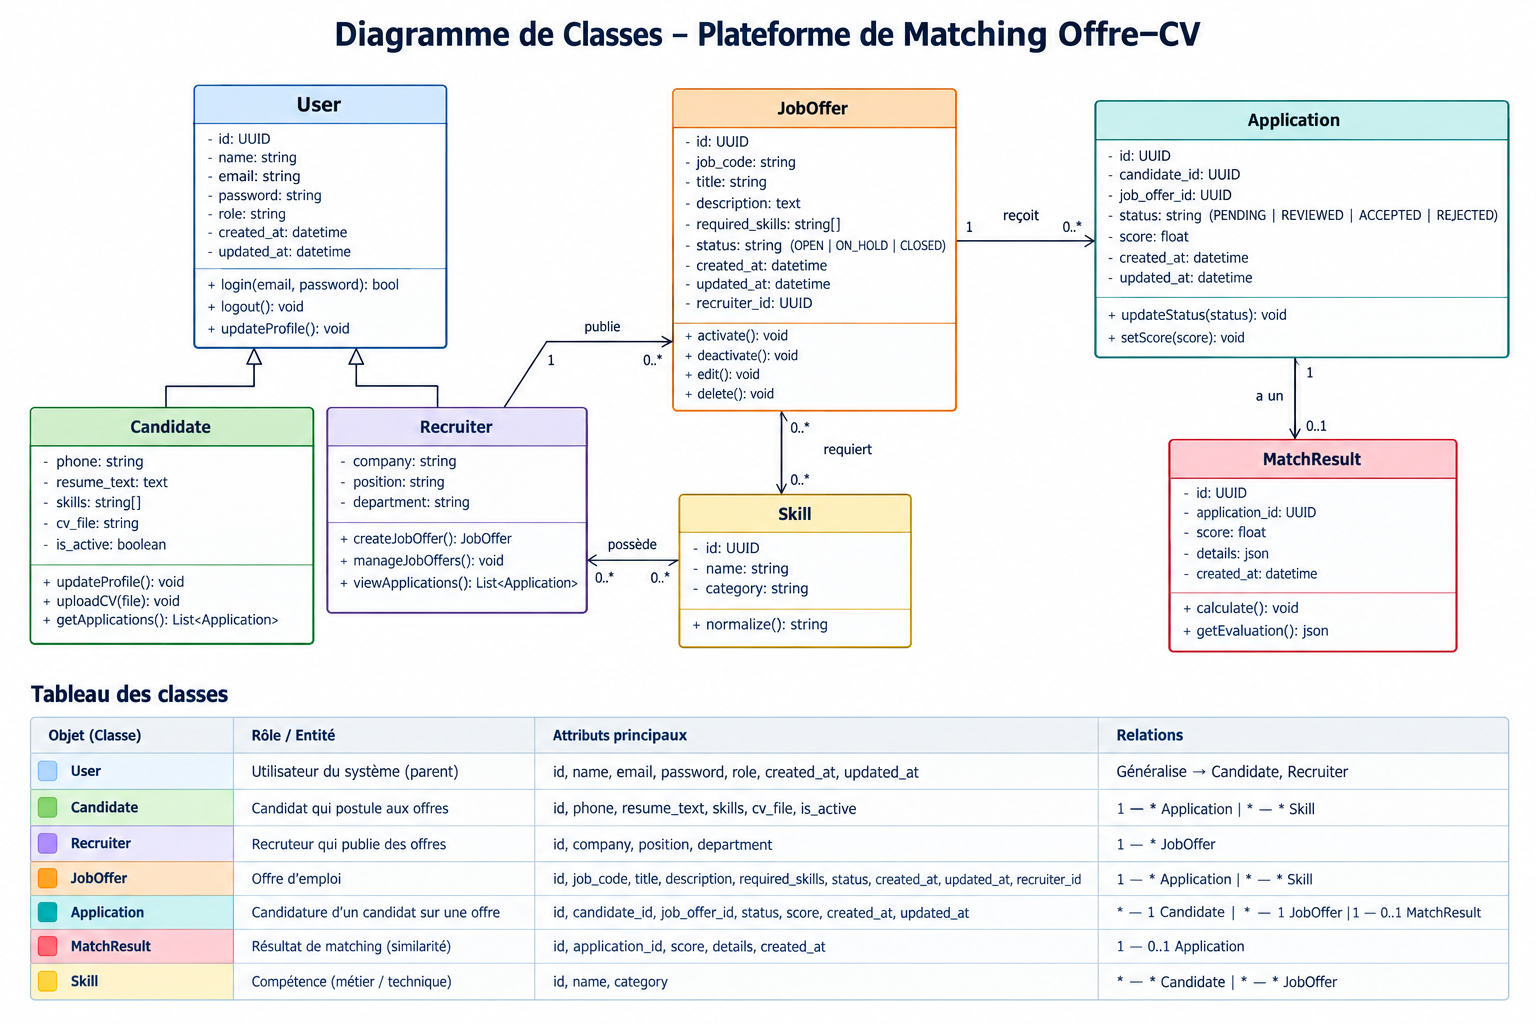
\includegraphics[width=.95\textwidth,height=.78\textheight,keepaspectratio]{img/diagrammes/classes.png}
\caption{Diagramme de classes métier simplifié de JobTest}
\label{fig:classes-globales}
\end{figure}

Un utilisateur recruteur possède des offres et des candidats. Un candidat peut regrouper plusieurs CV et plusieurs résultats de correspondance; chaque résultat se rattache au CV et à l'offre qui ont servi à son calcul. Les compétences sont normalisées dans \texttt{Skill} et reliées aux CV et aux offres par les tables d'association \texttt{cv\_skills} et \texttt{job\_skills}. Les chemins actuels d'évaluation conservent également le texte et les informations d'explication dans le résultat pour en permettre la consultation ultérieure.

\section{Conception dynamique -- diagrammes de séquence}

\subsection{Authentification du recruteur}
La connexion utilise le formulaire OAuth2 de FastAPI. Après vérification du mot de passe haché, l'API émet un JWT bearer. L'interface le stocke localement puis appelle \texttt{/auth/me} afin de charger le profil de session.

La figure~\ref{fig:seq-auth} détaille cet échange, depuis la soumission du formulaire jusqu'au chargement du profil.

\begin{figure}[htbp]
\centering
\begin{tikzpicture}[x=1cm,y=1cm]
  \node[seqpart] at (0,0) {Recruteur}; \node[seqpart] at (3.2,0) {Next.js};
  \node[seqpart] at (6.4,0) {FastAPI}; \node[seqpart] at (9.6,0) {Service\\d'authentification};
  \node[seqpart] at (12.8,0) {PostgreSQL};
  \foreach \x in {0,3.2,6.4,9.6,12.8} \draw[seqline] (\x,-.35)--(\x,-5.4);
  \draw[seqmsg] (0,-.8)--node[above]{identifiants} (3.2,-.8);
  \draw[seqmsg] (3.2,-1.35)--node[above]{POST /auth/login} (6.4,-1.35);
  \draw[seqmsg] (6.4,-1.9)--node[above]{vérifier mot de passe} (9.6,-1.9);
  \draw[seqmsg] (9.6,-2.45)--node[above]{rechercher e-mail} (12.8,-2.45);
  \draw[seqmsg] (12.8,-3.0)--node[above]{utilisateur} (9.6,-3.0);
  \draw[seqmsg] (9.6,-3.55)--node[above]{JWT bearer} (6.4,-3.55);
  \draw[seqmsg] (6.4,-4.1)--node[above]{jeton} (3.2,-4.1);
  \draw[seqmsg] (3.2,-4.65)--node[above]{GET /auth/me + bearer} (6.4,-4.65);
  \draw[seqmsg] (6.4,-5.15)--node[above]{profil de session} (3.2,-5.15);
\end{tikzpicture}

\caption{Séquence d'authentification du recruteur}
\label{fig:seq-auth}
\end{figure}

\subsection{Création d'une offre d'emploi}
L'écran des offres transmet le titre, la description, les compétences requises et l'état demandé. La route \texttt{/ui/job-offers} vérifie la présence du titre et de la description, associe l'offre au recruteur connecté et construit le code \texttt{JOB-AAAA-NNN} avant l'écriture en base.

La figure~\ref{fig:seq-offre} en retrace le déroulement.

\begin{figure}[htbp]
\centering
\begin{tikzpicture}[x=1cm,y=1cm]
  \node[seqpart] at (0,0) {Recruteur}; \node[seqpart] at (3.5,0) {Next.js};
  \node[seqpart] at (7,0) {FastAPI\\route /ui}; \node[seqpart] at (10.5,0) {PostgreSQL};
  \foreach \x in {0,3.5,7,10.5} \draw[seqline] (\x,-.35)--(\x,-5.0);
  \draw[seqmsg] (0,-.8)--node[above]{saisir offre} (3.5,-.8);
  \draw[seqmsg] (3.5,-1.4)--node[above]{POST /ui/job-offers} (7,-1.4);
  \draw[seqmsg] (7,-2.0)--node[above]{valider titre et description} (7.8,-2.0);
  \draw[seqmsg] (7,-2.6)--node[above]{compter les offres et générer\\JOB-AAAA-NNN} (10.5,-2.6);
  \draw[seqmsg] (7,-3.25)--node[above]{INSERT offre + recruteur\_id} (10.5,-3.25);
  \draw[seqmsg] (10.5,-3.85)--node[above]{offre créée} (7,-3.85);
  \draw[seqmsg] (7,-4.45)--node[above]{201 et offre sérialisée} (3.5,-4.45);
\end{tikzpicture}

\caption{Séquence de création d'une offre d'emploi}
\label{fig:seq-offre}
\end{figure}

\subsection{Évaluation d'un CV par rapport à une offre}
La figure~\ref{fig:seq-evaluation} représente le chemin canonique. Le CV est fourni comme texte ou par téléversement; dans ce dernier cas, le routeur extrait le texte du PDF ou du DOCX avant l'évaluation. L'offre doit appartenir au recruteur. Le service exécute les trois composantes, les agrège, applique les seuils et persiste un \texttt{MatchResult}.

Pour le modèle hybride par défaut, les scores élémentaires sont compris entre 0 et 1 et la formule effective est :
\[
S_h = 0{,}2S_{\mathrm{TF\text{-}IDF}} + 0{,}4S_{\mathrm{emb}} + 0{,}4S_{\mathrm{comp}}.
\]
Le pourcentage affiché vaut $100S_h$. Avec la configuration par défaut, le \texttt{DecisionEngine} produit \texttt{HIRE} si le score est supérieur ou égal à 75, \texttt{CONSIDER} s'il est compris entre 55 et strictement inférieur à 75, et \texttt{REJECT} en dessous de 55. Les seuils de session peuvent être transmis par l'interface, mais la configuration utilisée est enregistrée avec le résultat. Ce verdict est une recommandation algorithmique et non une décision de recrutement.

\begin{figure}[p]
\centering
\begin{tikzpicture}[x=1cm,y=1cm]
  \node[seqpart] at (0,0) {Recruteur}; \node[seqpart] at (2.7,0) {Next.js};
  \node[seqpart] at (5.4,0) {FastAPI}; \node[seqpart] at (8.1,0) {Service\\d'évaluation};
  \node[seqpart] at (10.8,0) {Layer 1}; \node[seqpart] at (13.5,0) {PostgreSQL};
  \foreach \x in {0,2.7,5.4,8.1,10.8,13.5} \draw[seqline] (\x,-.35)--(\x,-8.2);
  \draw[seqmsg] (0,-.8)--node[above]{choisir offre et CV} (2.7,-.8);
  \draw[seqmsg] (2.7,-1.35)--node[above]{POST /ui/evaluate\\ou /evaluate/file} (5.4,-1.35);
  \draw[seqmsg] (5.4,-1.9)--node[above]{valider CV et propriété de l'offre} (13.5,-1.9);
  \draw[seqmsg] (5.4,-2.5)--node[above]{texte normalisé + configuration} (8.1,-2.5);
  \draw[seqmsg] (8.1,-3.1)--node[above]{TF--IDF, embeddings,\\compétences} (10.8,-3.1);
  \draw[seqmsg] (10.8,-3.7)--node[above]{scores élémentaires} (8.1,-3.7);
  \draw[seqmsg] (8.1,-4.3)--node[above]{agréger 0,2 / 0,4 / 0,4} (10.8,-4.3);
  \draw[seqmsg] (10.8,-4.9)--node[above]{score hybride} (8.1,-4.9);
  \draw[seqmsg] (8.1,-5.5)--node[above]{décision, explication,\\recommandations} (10.8,-5.5);
  \draw[seqmsg] (8.1,-6.1)--node[above]{persist\_evaluation} (13.5,-6.1);
  \draw[seqmsg] (13.5,-6.7)--node[above]{MatchResult} (8.1,-6.7);
  \draw[seqmsg] (8.1,-7.3)--node[above]{résultat sérialisé} (5.4,-7.3);
  \draw[seqmsg] (5.4,-7.85)--node[above]{score, verdict, explication} (2.7,-7.85);
\end{tikzpicture}

\caption{Séquence centrale d'évaluation et de persistance d'un CV}
\label{fig:seq-evaluation}
\end{figure}
\clearpage

\subsection{Analyse approfondie avec Ollama}
Après le rendu de l'évaluation, le composant \texttt{DeepAnalysis} déclenche automatiquement un appel séparé pour l'identifiant du résultat; il peut aussi être relancé depuis l'interface. L'API reconstruit le contexte à partir du \texttt{MatchResult} sans recalculer la Layer~1. Ollama reçoit ce contexte structuré et doit fournir un JSON conforme. Une analyse réussie est ajoutée au résultat; sinon l'interface reçoit un état \texttt{disabled}, \texttt{unavailable}, \texttt{error} ou \texttt{inconsistent}. Dans tous les cas, le score et la décision de la Layer~1 restent inchangés.

L'enchaînement correspondant apparaît sur la figure~\ref{fig:seq-ollama}, où l'on voit que l'appel part d'un résultat déjà enregistré.

\begin{figure}[htbp]
\centering
\begin{tikzpicture}[x=1cm,y=1cm]
  \node[seqpart] at (0,0) {Next.js}; \node[seqpart] at (3.3,0) {FastAPI};
  \node[seqpart] at (6.6,0) {PostgreSQL}; \node[seqpart] at (9.9,0) {Service LLM};
  \node[seqpart] at (13.2,0) {Ollama local};
  \foreach \x in {0,3.3,6.6,9.9,13.2} \draw[seqline] (\x,-.35)--(\x,-6.5);
  \draw[seqmsg] (0,-.8)--node[above]{POST deep-analysis(match\_id)} (3.3,-.8);
  \draw[seqmsg] (3.3,-1.4)--node[above]{lire MatchResult possédé} (6.6,-1.4);
  \draw[seqmsg] (6.6,-2.0)--node[above]{scores, décision, explication} (3.3,-2.0);
  \draw[seqmsg] (3.3,-2.6)--node[above]{contexte structuré} (9.9,-2.6);
  \draw[seqmsg] (9.9,-3.2)--node[above]{/api/chat, format JSON} (13.2,-3.2);
  \draw[seqmsg] (13.2,-3.8)--node[above]{analyse JSON ou erreur} (9.9,-3.8);
  \draw[dashed,rounded corners=1pt] (2.5,-4.25) rectangle (10.7,-5.2);
  \node[anchor=west,font=\scriptsize] at (2.6,-4.42) {\textit{alt} statut \texttt{ok}};
  \draw[seqmsg] (9.9,-4.75)--node[above]{enveloppe valide} (3.3,-4.75);
  \draw[seqmsg] (3.3,-5.0)--node[below]{persister llm\_analysis\_json} (6.6,-5.0);
  \draw[seqmsg] (3.3,-5.75)--node[above]{statut contrôlé} (0,-5.75);
  \node[align=left,font=\scriptsize,anchor=west] at (.1,-6.35) {\textit{Sinon : disabled, unavailable, error ou inconsistent ; score et verdict inchangés.}};
\end{tikzpicture}

\caption{Séquence d'analyse approfondie, additive à la Layer~1}
\label{fig:seq-ollama}
\end{figure}

\subsection{Génération du rapport PDF}
Le téléchargement demande au serveur un document à partir du résultat, de l'explication et des recommandations déjà affichés. FastAPI délègue la mise en page au générateur ReportLab et retourne les octets PDF avec une en-tête de pièce jointe. Cette opération ne crée pas de nouvelle évaluation et ne modifie pas le résultat de correspondance.

La figure~\ref{fig:seq-pdf} montre la séquence suivie jusqu'au téléchargement du document.

\begin{figure}[htbp]
\centering
\begin{tikzpicture}[x=1cm,y=1cm]
  \node[seqpart] at (0,0) {Recruteur}; \node[seqpart] at (3.5,0) {Next.js};
  \node[seqpart] at (7,0) {FastAPI}; \node[seqpart] at (10.5,0) {Générateur\\ReportLab};
  \foreach \x in {0,3.5,7,10.5} \draw[seqline] (\x,-.35)--(\x,-4.7);
  \draw[seqmsg] (0,-.8)--node[above]{exporter le rapport} (3.5,-.8);
  \draw[seqmsg] (3.5,-1.45)--node[above]{POST /report/pdf\\résultat + explication} (7,-1.45);
  \draw[seqmsg] (7,-2.1)--node[above]{composer le document} (10.5,-2.1);
  \draw[seqmsg] (10.5,-2.75)--node[above]{octets PDF} (7,-2.75);
  \draw[seqmsg] (7,-3.4)--node[above]{application/pdf + pièce jointe} (3.5,-3.4);
  \draw[seqmsg] (3.5,-4.05)--node[above]{téléchargement} (0,-4.05);
\end{tikzpicture}

\caption{Séquence de génération et téléchargement d'un rapport PDF}
\label{fig:seq-pdf}
\end{figure}

\section{Conception des données}
Le modèle relationnel est porté par SQLAlchemy. \texttt{users.email}, \texttt{skills.name} et \texttt{job\_offers.job\_code} sont déclarés uniques. Les clés étrangères relient candidats et offres au recruteur, les CV aux candidats, puis les résultats à leur candidat, CV et offre. Les suppressions en cascade sont configurées entre candidat et CV, ainsi qu'entre candidat ou offre et résultats de correspondance.

Le résultat de correspondance est l'élément de traçabilité principal : il conserve les scores hybride, sémantique, lexical et compétences, la décision, les seuils utilisés, la version du modèle, la méthode et les poids. L'explication et les recommandations sont sérialisées dans \texttt{explanation\_json}; l'analyse approfondie valide est ajoutée dans \texttt{llm\_analysis\_json}. Les comparaisons de modèles et le benchmark de qualité ne créent pas de résultats persistants.

En développement, la valeur par défaut de \texttt{DATABASE\_URL} pointe vers SQLite et l'application active les clés étrangères SQLite. Dans le déploiement conteneurisé, cette variable cible PostgreSQL~16. Les mêmes modèles SQLAlchemy sont employés; la différence porte sur le moteur de base de données, non sur le modèle métier présenté.

\section{Principes de conception retenus}
\begin{itemize}
  \item \textbf{Séparation des responsabilités :} Next.js présente et collecte, FastAPI orchestre, les services calculent, SQLAlchemy persiste et Ollama interprète qualitativement.
  \item \textbf{Traçabilité et reproductibilité :} le résultat conserve les composantes, poids, version, méthode et seuils actifs lors de son calcul.
  \item \textbf{Isolation :} la pile Docker place PostgreSQL, FastAPI, Next.js et Ollama sur un réseau interne; seul Nginx expose le port~80.
  \item \textbf{Dégradation contrôlée :} l'indisponibilité, l'erreur ou l'incohérence de la Layer~2 est représentée par un état explicite, sans bloquer l'évaluation déterministe.
  \item \textbf{Responsabilité humaine :} la décision \texttt{HIRE}/\texttt{CONSIDER}/\texttt{REJECT} facilite l'examen d'un dossier; le recruteur demeure responsable de la décision finale.
\end{itemize}

\section*{Conclusion}
\addcontentsline{toc}{section}{Conclusion}
La conception de JobTest articule une interface Next.js, une API FastAPI, une persistance relationnelle et deux couches d'intelligence aux rôles distincts. Les diagrammes ont montré la conservation d'un résultat traçable, depuis l'authentification jusqu'au rapport et à l'analyse approfondie. Le chapitre suivant détaillera la conception et l'évaluation du moteur intelligent, notamment ses composantes de correspondance et ses résultats de validation.

        \clearpage
        \chapter{Conception et évaluation du moteur intelligent}
\label{chap:moteur-intelligent}
\newpage

\section*{Introduction}
\addcontentsline{toc}{section}{Introduction}

Le moteur de rapprochement de JobTest relie un CV et une offre à une recommandation exploitable par un recruteur. Il ne prédit ni une embauche ni une décision autonome~: il mesure une compatibilité textuelle et métier, la calibre, puis applique des règles explicites. Ce chapitre décrit les composants réellement implémentés et leur évaluation quantitative reproductible sur le corpus synthétique du projet.

\section{Objectifs et principes de conception}

Le moteur doit accepter des CV hétérogènes, confronter vocabulaire et sens général, signaler les compétences manquantes et rendre le résultat vérifiable. Le choix retenu est une fusion tardive~: chaque composant conserve son score avant agrégation. Deux couches sont séparées. La couche~1 produit le score, la décision et les justifications déterministes. La couche~2, optionnelle, enrichit seulement l'affichage par une analyse locale~; elle ne modifie ni score ni décision.

La figure~\ref{fig:chap4-pipeline} résume cet enchaînement et la place qu'y occupe la couche optionnelle.

\begin{figure}[htbp]
  \centering
  \resizebox{\textwidth}{!}{%
  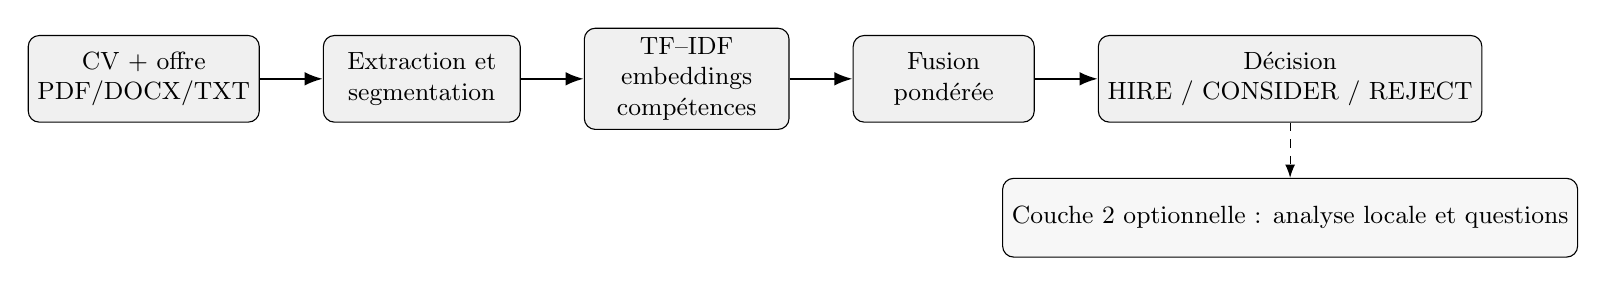
\begin{tikzpicture}[node distance=7mm and 8mm,every node/.style={font=\small,align=center},>=Latex]
    \node[draw,rounded corners,fill=gray!12,minimum width=23mm,minimum height=11mm] (cv) {CV + offre\\PDF/DOCX/TXT};
    \node[draw,rounded corners,fill=gray!12,minimum width=25mm,minimum height=11mm,right=of cv] (parse) {Extraction et\\segmentation};
    \node[draw,rounded corners,fill=gray!12,minimum width=26mm,minimum height=11mm,right=of parse] (models) {TF--IDF\\embeddings\\compétences};
    \node[draw,rounded corners,fill=gray!12,minimum width=23mm,minimum height=11mm,right=of models] (fusion) {Fusion\\pondérée};
    \node[draw,rounded corners,fill=gray!12,minimum width=27mm,minimum height=11mm,right=of fusion] (decision) {Décision\\HIRE / CONSIDER / REJECT};
    \node[draw,rounded corners,fill=gray!6,minimum width=35mm,minimum height=10mm,below=of decision] (llm) {Couche~2 optionnelle~: analyse locale et questions};
    \draw[->,thick] (cv)--(parse); \draw[->,thick] (parse)--(models);
    \draw[->,thick] (models)--(fusion); \draw[->,thick] (fusion)--(decision);
    \draw[->,dashed] (decision)--(llm);
  \end{tikzpicture}
  }
  \caption{Pipeline de rapprochement de JobTest}
  \label{fig:chap4-pipeline}
\end{figure}

\section{Prétraitement et structuration des documents}

L'extraction privilégie \texttt{pdfplumber} pour les PDF et bascule sur \texttt{PyPDF2} en cas d'indisponibilité~; les fichiers DOCX sont lus avec \texttt{python-docx}, avec un repli XML. Le texte est nettoyé des URL, courriels, numéros de téléphone, retours superflus et artefacts de césure. La normalisation disponible applique, lorsque les modèles spaCy sont installés, tokenisation, lemmatisation et filtrage des mots-outils~; un repli par expressions régulières et lemmatisation légère maintient le traitement sinon.

Le CV est ensuite segmenté par intitulés français et anglais~: profil, expérience, compétences, formation, langues, certifications et projets. Cette structure n'est pas une interprétation humaine du dossier~; elle permet notamment de pondérer l'expérience distinctement des compétences.

\section{Similarité lexicale TF--IDF}

Le premier composant vectorise CV et offre avec \texttt{TfidfVectorizer}. La configuration implémentée utilise des $n$-grammes de 1 à 3 termes, au plus 10\,000 caractéristiques et une fréquence de terme sous-linéaire. TF--IDF valorise les termes discriminants~; la similarité cosinus compare les vecteurs issus des deux textes \cite{scikit_tfidf,scikit_cosine} :
\[
 \operatorname{tfidf}(t,d)=\operatorname{tf}(t,d)\log\left(\frac{N+1}{\operatorname{df}(t)+1}\right)+1,
 \qquad S_{\mathrm{TFIDF}}=\frac{\vec v_{CV}\cdot\vec v_{offre}}{\lVert\vec v_{CV}\rVert\lVert\vec v_{offre}\rVert}.
\]
Cette composante est lisible lorsque les mêmes technologies sont citées, mais elle reste sensible aux synonymes et aux reformulations.

\section{Similarité sémantique par embeddings}

Le deuxième composant encode les textes avec Sentence-Transformers lorsqu'il est disponible. Le modèle anglais configuré par défaut est \texttt{all-mpnet-base-v2}. Le modèle multilingue est identifié dans la configuration par :
\begin{center}
  \small\texttt{paraphrase-multilingual-mpnet-base-v2}
\end{center}
\texttt{HashingVectorizer} constitue le repli local en cas de chargement impossible. Les représentations de phrases et leur comparaison cosinus s'appuient sur le principe de Sentence-BERT \cite{reimers2019sbert}.

Les similitudes anglaise et multilingue sont moyennées. Une similitude par sections reçoit les poids expérience 0,40~; compétences 0,30~; résumé 0,15~; formation 0,10~; langues 0,05. Le composant retourne donc :
\[
 S_{\mathrm{emb}}=0{,}7\left(0{,}5s_{en}+0{,}5s_{multi}\right)+0{,}3s_{sections}.
\]
La pondération rend l'expérience et les compétences plus influentes sans prétendre représenter une adéquation humaine complète.

\section{Rapprochement structuré des compétences}

Le troisième composant exploite le dictionnaire versionné du projet. Il détecte les compétences techniques et comportementales, les certifications, les variantes et des $n$-grammes normalisés. Les termes de nécessité, tels que \emph{required}, \emph{must} ou \emph{obligatoire}, signalent des compétences critiques.

Soient $H$ et $S$ les recouvrements techniques et comportementaux. La base répartit les poids 0,70 et 0,30 entre les catégories présentes. Elle reçoit un bonus de domaine de 0,05, un bonus de certification plafonné à 0,10, puis une pénalité plafonnée à 0,20 pour les compétences critiques absentes :
\[
 S_{\mathrm{skill}}=\operatorname{clip}\left(S_{base}+0{,}05I_{domaine}+\min(0{,}10,0{,}03n_{cert})-0{,}20\frac{n_{critiques\ absentes}}{n_{critiques}},0,1\right).
\]
Il restitue aussi les compétences trouvées, manquantes et critiques~: ces éléments constituent la justification métier principale.

\subsection{Contrôle des preuves avant le calcul}

Un CV peut citer les compétences d'une offre sans démontrer qu'elles ont été pratiquées. Avant le calcul, la version finale applique donc trois contrôles explicables, dont le résultat accompagne chaque évaluation.
\begin{itemize}
  \item \textbf{Texte recopié de l'offre.} Toute séquence d'au moins huit mots consécutifs également présente dans l'offre est retirée du CV avant le calcul des trois composantes. Sur les 12\,000 paires du corpus, la plus longue séquence commune légitime compte sept mots~: aucune paire authentique n'est modifiée.
  \item \textbf{Mentions niées.} Une compétence citée dans une proposition négative (« aucune expérience en Kubernetes », \emph{no experience with Docker}) n'est pas comptée, et la proposition correspondante est retirée du texte utilisé pour TF--IDF et les embeddings.
  \item \textbf{Compétences déclarées ou démontrées.} Une compétence qui n'apparaît que dans une liste (section « Compétences », « Technologies » ou ligne « Skills~: \ldots ») est dite déclarée~; elle compte pour moitié dans la couverture. Une compétence citée dans l'expérience, les projets, le profil ou une certification est dite démontrée. Lorsque le CV ne comporte aucun intitulé de section reconnaissable, la distinction est impossible et toutes les mentions sont traitées comme démontrées.
\end{itemize}
Ces contrôles ne modifient aucun score des 3\,600 paires authentiques de validation et de test~; ils agissent sur les CV qui répètent l'offre ou qui reposent sur des listes déclaratives.

\section{Fusion hybride et décision}

La configuration documentée n'apprend pas les poids de fusion~; elle les fixe ainsi :
\[
 S_{hybride}=0{,}2S_{\mathrm{TFIDF}}+0{,}4S_{\mathrm{emb}}+0{,}4S_{\mathrm{skill}}.
\]
Elle donne le même poids à la proximité sémantique et à la couverture explicite des compétences. Le score brut $S_{hybride}$ reste toutefois une combinaison de similarités qui n'ont pas d'échelle commune~: la similarité cosinus de deux documents différents dépasse rarement 0,8, le recouvrement TF--IDF reste en général sous 0,5, et la fusion n'atteint pas 0,75 même lorsque chaque composante est à son maximum observé. Lu directement en pourcentage contre des bornes à 55 et 75, ce score ne produirait presque que des verdicts \texttt{REJECT}.

La version finale interpose donc une calibration versionnée entre le score brut et le score affiché. Il s'agit d'une transformation monotone, linéaire par morceaux, définie par trois points d'ancrage appris sur la partition de validation (Tableau~\ref{tab:chap4-calibration}). Elle préserve l'ordre des scores bruts jusqu'au plafond. Au-delà de 0,6126, en revanche, tous les scores affichés valent 100~: deux scores bruts distincts peuvent donc recevoir le même score affiché, et l'arrondi au dixième produit le même effet à plus petite échelle. Les AUC rapportées dans ce chapitre sont pour cette raison calculées sur les scores bruts, et le classement multi-CV départage les égalités par le score brut. La calibration laisse les sous-scores bruts inchangés dans l'explication. Chaque résultat enregistre le score brut, le score affiché, la version de calibration et les seuils appliqués.

\begin{table}[htbp]
  \centering
  \caption{Ancrages de la calibration}
  \label{tab:chap4-calibration}
  \begin{tabular}{|l|r|r|}
    \hline
    Point d'ancrage & Score brut $S_{hybride}$ & Score affiché \\
    \hline
    Origine & 0 & 0 \\
    \hline
    Frontière \texttt{REJECT}/\texttt{CONSIDER} & 0,2633 & 55 \\
    \hline
    Frontière \texttt{CONSIDER}/\texttt{HIRE} & 0,3638 & 75 \\
    \hline
    Plafond (maximum observé en validation) & 0,6126 & 100 \\
    \hline
  \end{tabular}
\end{table}

Les deux frontières sont choisies sur la validation en maximisant le macro-F1 du verdict à trois classes, comparé aux trois catégories du générateur~: paires sans rapport, profils transférables et adéquations fortes. Pour l'exemple $(S_{\mathrm{TFIDF}},S_{\mathrm{emb}},S_{\mathrm{skill}})=(0{,}10;0{,}55;0{,}20)$, le score brut vaut $0{,}32$ et le score affiché $66{,}3$. Les méthodes isolées, sélectionnables dans l'interface, disposent chacune de leurs propres ancrages.

Le \texttt{DecisionEngine} applique ensuite au score affiché les bandes du Tableau~\ref{tab:chap4-seuils}, réglables par le recruteur. Une règle de prudence complète ces bandes~: lorsque le texte recopie l'offre, ou lorsque moins de la moitié des compétences correspondantes sont démontrées, le verdict \texttt{HIRE} est remplacé par \texttt{CONSIDER}, avec une justification invitant à vérifier l'expérience. Le score affiché n'est pas modifié.

\begin{table}[htbp]
  \centering
  \caption{Bandes de décision par défaut}
  \label{tab:chap4-seuils}
  \begin{tabular}{|l|l|l|}
    \hline
    Score affiché & Recommandation & Interprétation opérationnelle \\
    \hline
    $[75,100]$ & \texttt{HIRE} & adéquation forte à examiner en priorité \\
    \hline
    $[55,75[$ & \texttt{CONSIDER} & profil à examiner avec réserves explicites \\
    \hline
    $[0,55[$ & \texttt{REJECT} & adéquation insuffisante selon les signaux disponibles \\
    \hline
  \end{tabular}
\end{table}

Ces ancrages sont appris sur des étiquettes synthétiques. Ils alignent les bandes affichées sur les classes du banc d'essai~; ils ne constituent pas une politique d'embauche validée. La confiance présentée par le moteur est une distance au seuil le plus proche, et non une probabilité d'embauche.

\section{Explicabilité et couche d'analyse locale}

La couche~1 conserve les sous-scores, poids, décision, compétences trouvées ou absentes, compétences critiques et expérience détectée. L'interface peut donc formuler une justification contrôlable, par exemple l'absence de Docker et Kubernetes parmi les prérequis.

Après ce résultat, l'interface peut demander une analyse approfondie. Le service transmet alors le texte source et ce contexte déterministe à un modèle local configuré par défaut comme \texttt{qwen2.5:1.5b}, exécuté via Ollama. La réponse structurée propose trajectoire, alertes, justification, recommandations et questions d'entretien. Les états \texttt{disabled}, \texttt{unavailable}, \texttt{error} et \texttt{inconsistent} sont contrôlés sans bloquer la couche~1~; une incohérence générative ne révise donc jamais la recommandation.

\subsection{Construction du contexte et format de réponse}

L'appel au modèle local n'est pas une requête libre. Le service assemble un contexte à partir du résultat déjà persistant~: score calibré global, sous-scores des trois composantes, décision retenue et libellé de sa bande, compétences trouvées, compétences absentes et compétences critiques manquantes. Le modèle reçoit donc le verdict comme une donnée d'entrée à commenter, et non comme une question à trancher. Le texte du CV et celui de l'offre accompagnent ce contexte pour que l'analyse puisse s'appuyer sur le contenu réel du dossier.

La réponse attendue est un objet structuré comportant cinq parties~: une lecture de la trajectoire professionnelle, les points d'attention, une justification du positionnement, des recommandations et des questions d'entretien. Cette contrainte de format sert deux objectifs. Elle rend la réponse exploitable par l'interface sans analyse de texte libre, et elle interdit au modèle de produire un score concurrent~: aucun champ ne prévoit de note chiffrée ni de verdict. Une réponse qui ne se conforme pas au schéma attendu est rejetée plutôt que corrigée, et l'état correspondant est remonté à l'interface.

\subsection{Garde-fou de cohérence et tentative d'injection}

La contrainte de format ne suffit pas. Un petit modèle exécuté sur processeur peut respecter la structure demandée tout en énonçant une appréciation qui contredit la décision statistique~: décrire comme un excellent profil un dossier que le moteur a classé en \texttt{REJECT} avec des compétences critiques absentes. Une telle réponse n'est pas seulement inexacte, elle est trompeuse, puisqu'elle apparaît à côté du verdict qu'elle dément.

Le service applique donc un contrôle de cohérence sur les cas de faible adéquation. Le texte produit est examiné à la recherche d'affirmations positives incompatibles avec le verdict, en tenant compte des négations pour éviter de sanctionner une formulation telle que « ce n'est pas un profil adapté ». Lorsqu'une contradiction est détectée, le service relance une fois le modèle avec un rappel explicite du verdict à respecter. Si la seconde réponse contredit encore la décision, l'analyse est abandonnée et l'état \texttt{inconsistent} est retourné~: le système préfère ne rien afficher plutôt qu'afficher un commentaire qui affaiblirait la recommandation. C'est un comportement de défaillance fermée, cohérent avec le principe selon lequel la couche~2 ne peut jamais réviser la couche~1.

Ce garde-fou joue également un rôle de sécurité. Le texte d'un CV est fourni par un tiers et se retrouve intégré au message envoyé au modèle~; un candidat averti pourrait y insérer des instructions destinées à l'influencer, par exemple une consigne affirmant qu'il s'agit d'un profil parfait et qu'aucune réserve ne doit être émise. L'audit de sécurité du projet a retenu ce scénario comme un risque réel. Deux propriétés le contiennent. D'une part, le score et la décision sont calculés par le moteur déterministe avant tout appel au modèle~: une injection réussie ne peut pas modifier le verdict, seulement le commentaire qui l'accompagne. D'autre part, c'est précisément sur les dossiers faiblement classés qu'une injection aurait un intérêt, et c'est là que le contrôle de cohérence est actif~: un texte trop favorable sur un dossier rejeté conduit au rejet de l'analyse. La protection n'est pas absolue, mais la surface exposée se limite à du texte consultatif, jamais à la recommandation elle-même.

\section{Jeu de données et protocole expérimental}

L'évaluation utilise \texttt{cv\_job\_dataset.csv}, généré localement avec la graine 42. Il contient 12\,000 paires CV--offre synthétiques, plusieurs domaines et niveaux d'expérience, des textes français et anglais, des abréviations, fautes de frappe, compétences obsolètes et offres contradictoires. Les étiquettes positives regroupent les cas de forte et de transférable adéquation générés~; elles ne sont pas des décisions de recrutement observées.

\subsection{Pourquoi un corpus synthétique}

Le choix d'évaluer le moteur sur des documents générés plutôt que sur de vraies candidatures mérite d'être justifié, car il conditionne la portée de tous les chiffres qui suivent. Cinq raisons l'ont motivé.

La première est l'absence de corpus disponible. Aucun ensemble de CV réels appariés à des offres, en nombre suffisant et en accès autorisé, n'a pu être réuni dans le cadre de ce stage. Les quelques dossiers accessibles se comptaient en dizaines, ce qui n'aurait permis ni un partitionnement en trois sous-ensembles, ni une mesure stable~: sur un échantillon aussi réduit, un écart de quelques paires suffit à déplacer un F1 de plusieurs points, et la comparaison entre quatre méthodes n'aurait plus été interprétable.

La deuxième raison est juridique et éthique. Un CV réel est une donnée à caractère personnel, et son usage dans un travail académique suppose une base légale, une information des personnes et une durée de conservation définie, comme le rappelle la section consacrée à ce sujet au chapitre~\ref{chap:tests-securite}. Construire un corpus de test à partir de candidatures authentiques aurait demandé des démarches que le cadre du projet ne permettait pas, et aurait introduit dans le dépôt des données qu'il aurait fallu ensuite protéger, anonymiser puis supprimer.

La troisième tient à la qualité d'extraction. Les CV réels circulent dans des formats hétérogènes, parfois exportés depuis un traitement de texte, parfois scannés, souvent mis en page sur plusieurs colonnes ou dans des tableaux. L'extraction de texte y échoue partiellement~: ordre de lecture inversé, colonnes fusionnées, caractères manquants, sections illisibles. Un échec de ce type se répercute sur les trois composantes du score. En travaillant sur des documents dont le contenu textuel est maîtrisé, l'évaluation mesure le rapprochement lui-même et non la qualité variable d'une chaîne d'extraction, dont le comportement est vérifié séparément par les tests de \texttt{parsing}.

La quatrième raison est l'absence de vérité de terrain exploitable. Même avec des CV réels, il aurait fallu disposer, pour chaque paire, d'un jugement fiable indiquant si le profil convient à l'offre. Ce jugement n'existe pas dans un dossier de candidature~: une embauche dépend d'entretiens, de disponibilités et d'arbitrages qui ne figurent nulle part dans le document. Il aurait donc fallu faire annoter des milliers de paires par des recruteurs, ce qui dépassait largement le périmètre du stage. Le générateur, lui, connaît par construction la raison pour laquelle une paire est compatible ou non, ce qui fournit une étiquette cohérente avec le critère évalué.

La cinquième est la reproductibilité. Le corpus est produit par un script du dépôt avec une graine fixée à 42~: n'importe quel lecteur peut le régénérer à l'identique, relancer le banc d'essai et retrouver les valeurs du Tableau~\ref{tab:chap4-resultats}. Un jeu de CV réels, même anonymisé, n'aurait pas pu être distribué avec le code.

J'ai écrit le générateur pour ne pas produire des documents trop faciles. Chaque CV est assemblé à partir du dictionnaire de compétences du projet, avec un domaine et un niveau d'expérience, puis dégradé volontairement~: abréviations, fautes de frappe, technologies obsolètes, formulations en français ou en anglais. Des paires contradictoires sont également générées, où le vocabulaire se recoupe alors que le profil ne correspond pas, précisément pour empêcher qu'un simple recouvrement de mots suffise. La figure~\ref{fig:chap4-exemple-cv} montre l'un de ces documents.

\begin{figure}[H]
  \centering
  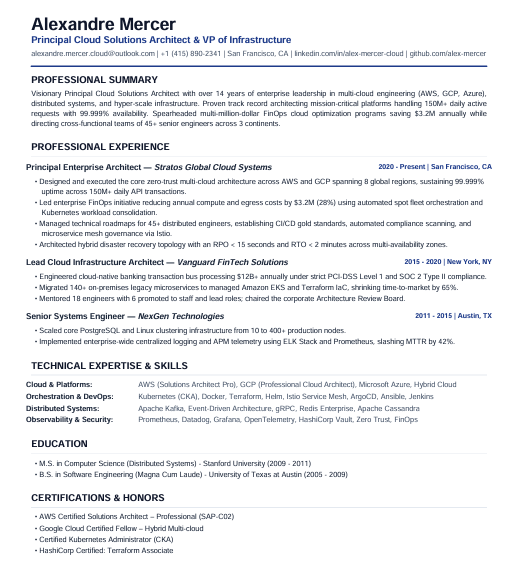
\includegraphics[width=.55\textwidth]{img/ai/example_cv.png}
  \caption{Exemple de CV synthétique}
  \label{fig:chap4-exemple-cv}
\end{figure}

Il faut néanmoins nommer ce que ce choix coûte, et le chapitre y revient dans sa section consacrée aux limites. Un document généré reste plus régulier qu'une candidature authentique~: la longueur varie peu, la structure est constante, le vocabulaire provient d'un dictionnaire fini et aucune trajectoire atypique n'y figure. Les résultats obtenus mesurent donc la capacité du moteur à distinguer des profils sur un matériau contrôlé~; ils ne préjugent pas de son comportement sur des CV réels, dont la validation reste la première étape à mener avant tout usage opérationnel.

\subsection{Partitionnement et métriques}

La séparation est stratifiée par étiquette et domaine, puis vérifiée par groupe de paire CV--offre normalisée~: 8\,400 paires pour l'apprentissage, 1\,800 pour la validation et 1\,800 pour le test final. Les poids de fusion sont fixés avant l'évaluation, le vocabulaire TF--IDF est appris sur l'apprentissage seul, les seuils binaires de chaque méthode sont sélectionnés sur la validation en maximisant le F1, et les ancrages de calibration le sont en maximisant le macro-F1 à trois classes. Les métriques sont ensuite calculées sur le test isolé. Je n'ai choisi aucun poids, seuil ni ancrage sur le test. J'ai toutefois consulté ce test à plusieurs reprises au cours du projet~: les chiffres finaux n'ont pas été réglés sur lui, mais il n'est plus strictement neuf, ce qui laisse un risque résiduel d'optimisme. Une alerte automatique signale toute méthode qui présenterait une AUC élevée et un F1 quasi nul, symptôme d'un seuil mal placé. Le partitionnement réduit la fuite de paires identiques, sans remplacer une validation externe réelle.

Les métriques sont l'exactitude, la précision, le rappel, le F1, l'AUC-ROC, l'aire précision--rappel, le kappa de Cohen et la matrice de confusion, selon les définitions de scikit-learn \cite{scikit_metrics}. Deux familles sont distinguées~: le F1 binaire, qui oppose les paires positives aux autres à un seuil donné, et le macro-F1 à trois classes, moyenne des F1 de \texttt{REJECT}, \texttt{CONSIDER} et \texttt{HIRE}, qui évalue les verdicts affichés. Ces deux mesures ne sont pas comparables entre elles. Le F1 équilibre précision et rappel :
\[
 F1=2\frac{\mathrm{precision}\times\mathrm{rappel}}{\mathrm{precision}+\mathrm{rappel}}.
\]

\section{Résultats et analyse comparative}

Le Tableau~\ref{tab:chap4-resultats} reproduit les résultats enregistrés sur les 1\,800 paires de test. Les seuils affichés sont des points de fonctionnement expérimentaux et non les seuils \texttt{HIRE}/\texttt{CONSIDER}/\texttt{REJECT} de l'interface.

\begin{table}[htbp]
  \centering
  \small
  \caption{Qualité du score brut (F1 binaire)}
  \label{tab:chap4-resultats}
  \begin{tabular}{|l|r|r|r|r|r|r|}
    \hline
    Méthode & Seuil & Exact. & Préc. & Rappel & F1 & AUC-ROC \\
    \hline
    TF--IDF & 0,04 & 0,93 & 0,93 & 0,97 & 0,95 & 0,98 \\
\hline
    Embeddings & 0,54 & 0,78 & 0,81 & 0,89 & 0,85 & 0,81 \\
\hline
    Compétences & 0,00 & 0,89 & 0,89 & 0,97 & 0,93 & 0,95 \\
\hline
    Hybride & 0,26 & 0,91 & 0,94 & 0,93 & 0,93 & 0,96 \\
    \hline
  \end{tabular}
\end{table}

La figure~\ref{fig:chap4-roc} présente les courbes ROC des scores bruts sur les mêmes paires. Elles mesurent la qualité du classement indépendamment de tout seuil~: l'AUC de la fusion (0,964) reste inférieure à celle de TF--IDF (0,979), et les embeddings seuls classent nettement moins bien (0,811). Ces courbes ne disent rien des verdicts affichés, évalués plus loin.

\begin{figure}[htbp]
  \centering
  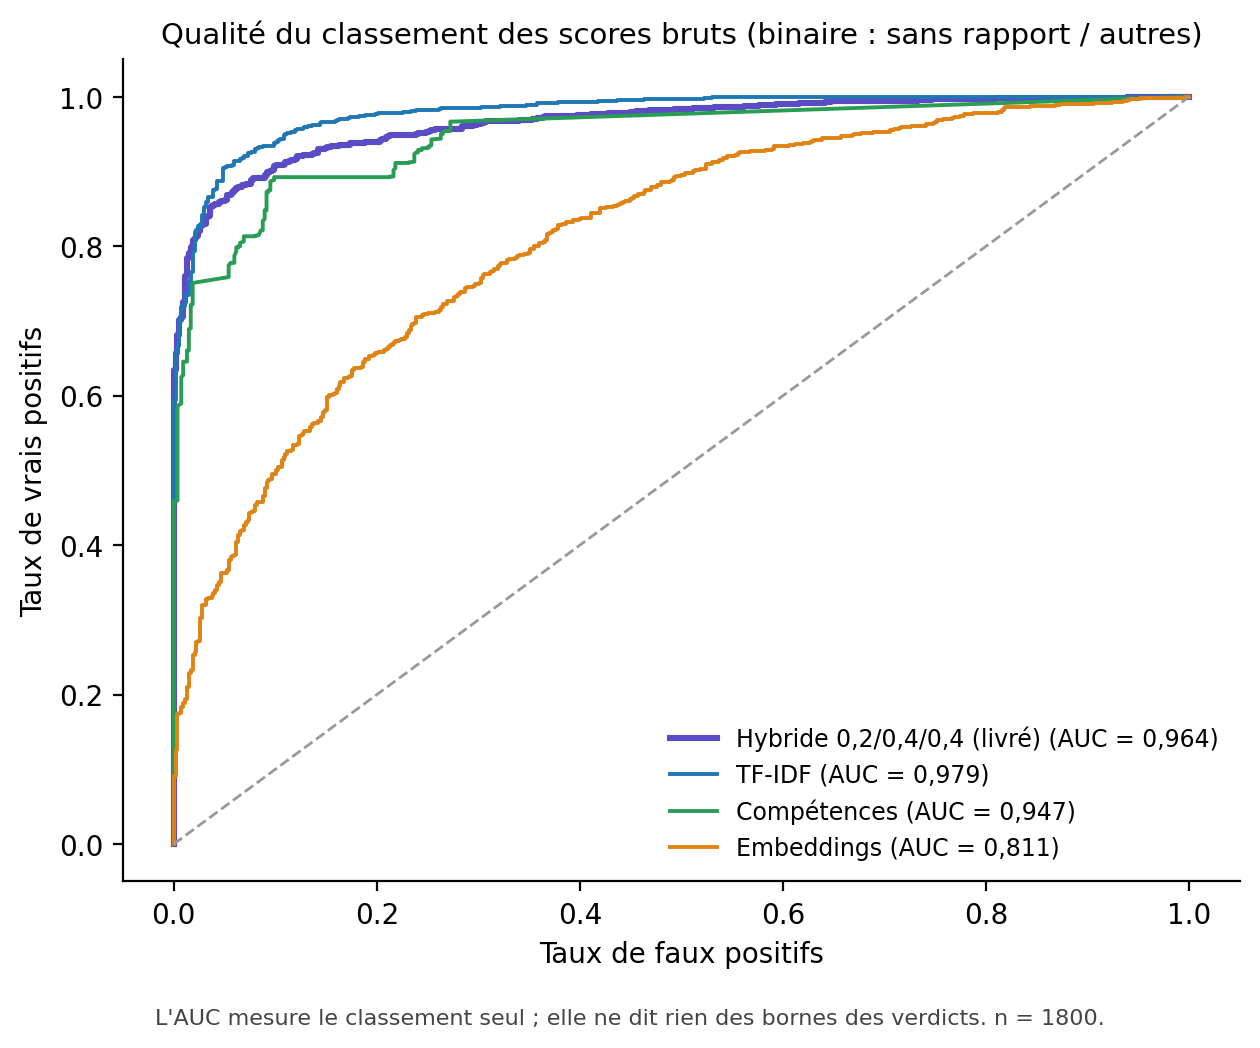
\includegraphics[width=.72\textwidth]{img/ai/eval_roc_raw.png}
  \caption{Courbes ROC des scores bruts}
  \label{fig:chap4-roc}
\end{figure}

La figure~\ref{fig:chap4-brut-classes} relie le score brut de la fusion aux trois classes synthétiques et aux deux ancrages de la calibration, qui deviennent 55 et 75 sur l'échelle affichée. Les paires sans rapport se concentrent sous le premier ancrage et la plupart des adéquations fortes au-dessus du second. Les profils transférables chevauchent les deux autres classes, ce qui annonce la difficulté de la classe intermédiaire.

\begin{figure}[htbp]
  \centering
  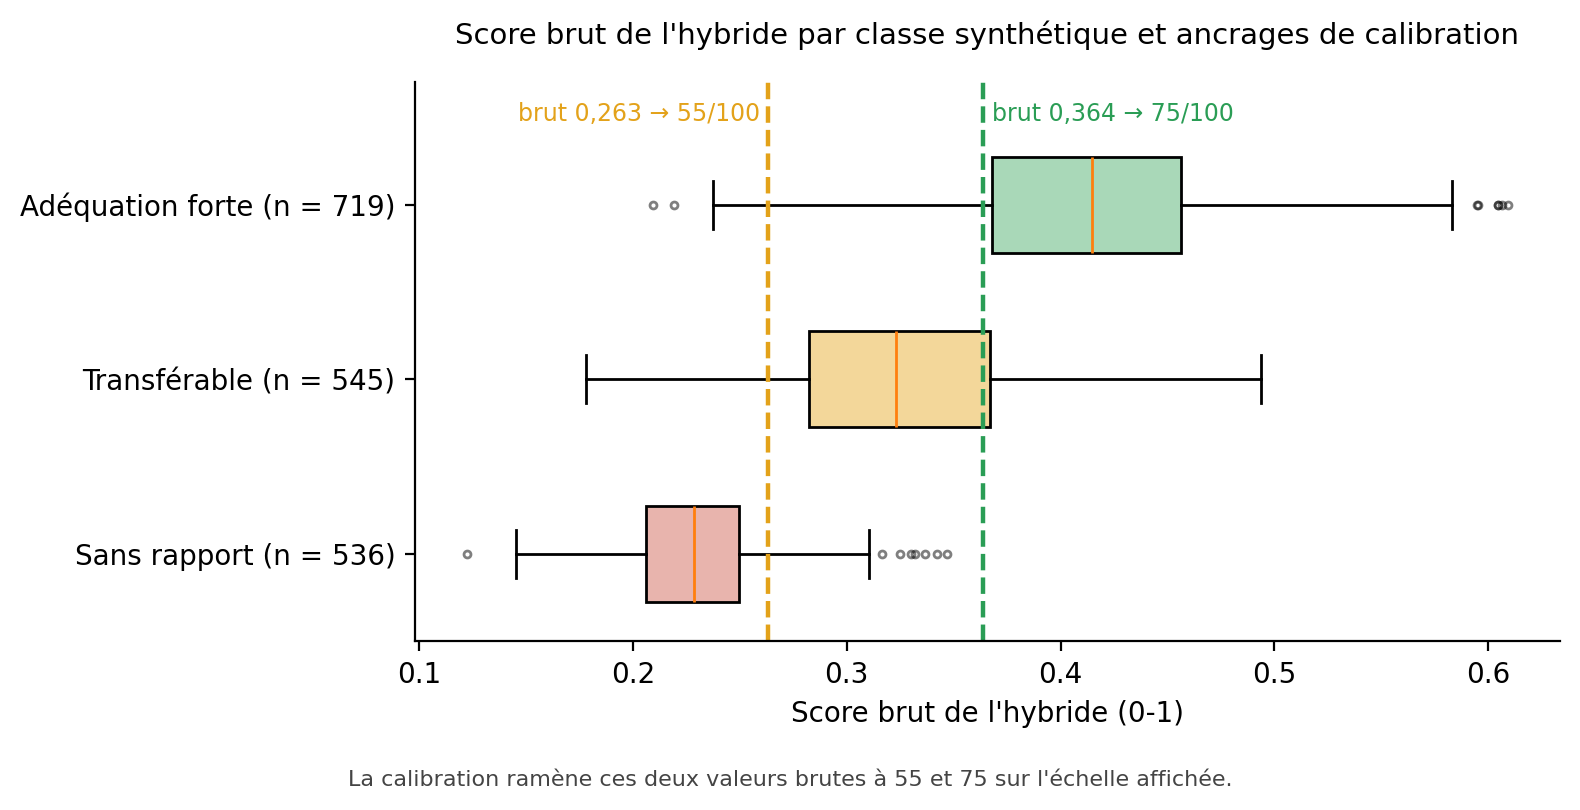
\includegraphics[width=.9\textwidth]{img/ai/eval_hybrid_raw_by_class.png}
  \caption{Score brut de la fusion par classe}
  \label{fig:chap4-brut-classes}
\end{figure}

TF--IDF obtient le meilleur F1 dans ce protocole~: $F1=0{,}95$ (intervalle bootstrap à 95~\%~: 0,941--0,959), contre $F1=0{,}93$ (0,924--0,944) et $AUC=0{,}96$ pour la fusion. Sur les mêmes 1\,800 paires, chacune lue à son propre seuil de validation, TF--IDF classe correctement 108 paires que la fusion manque, et l'inverse se produit pour 73 paires~; le test de McNemar donne $p\approx0{,}011$. Ce protocole ne permet donc pas de revendiquer une supériorité mesurée de l'hybride~: la différence observée va dans le sens inverse. Elle ne démontre pas pour autant une supériorité générale du lexical, car le générateur construit CV et offres à partir d'un vocabulaire contrôlé et partagé, ce qui favorise le recouvrement des termes. La fusion est retenue pour des raisons que ce benchmark ne mesure pas~: la justification par compétences restituée au recruteur et une moindre sensibilité à la reformulation, observée sur l'expérience contrôlée du Tableau~\ref{tab:chap4-bug4}. Le temps moyen mesuré est 55,85~ms par paire pour la fusion, contre 921,60~ms pour les embeddings seuls dans cet environnement.

\subsection*{Verdicts affichés par la version finale}
\addcontentsline{toc}{subsection}{Verdicts affichés par la version finale}

Le Tableau~\ref{tab:chap4-resultats} mesure la capacité de discrimination du score brut. Le Tableau~\ref{tab:chap4-verdicts} évalue ce que voit le recruteur, c'est-à-dire les verdicts \texttt{REJECT}, \texttt{CONSIDER} et \texttt{HIRE}, sur les mêmes 1\,800 paires de test. Celles-ci comptent 536 paires sans rapport, 545 profils transférables et 719 adéquations fortes.

\begin{table}[H]
  \centering
  \footnotesize
  \caption{Qualité des verdicts affichés}
  \label{tab:chap4-verdicts}
  \begin{tabular}{|>{\raggedright\arraybackslash}p{3.7cm}|>{\centering\arraybackslash}p{2.5cm}|>{\centering\arraybackslash}p{1.2cm}|>{\centering\arraybackslash}p{1.7cm}|>{\centering\arraybackslash}p{1.1cm}|>{\centering\arraybackslash}p{2.3cm}|}
    \hline
    Configuration & Macro-F1 3 classes [IC 95~\%] & F1 \texttt{HIRE} & F1 binaire \texttt{CONSIDER} ou mieux & Kappa q. & Verdicts R / C / H \\
    \hline
    \textbf{Hybride calibré (version finale)} & \textbf{0,740} [0,720--0,760] & 0,782 & 0,934 & 0,799 & 548 / 557 / 695 \\
    \hline
    TF--IDF seul, calibré & 0,746 [0,726--0,765] & 0,758 & 0,950 & 0,797 & 471 / 641 / 688 \\
    \hline
    Fusion apprise 0,75 / 0,05 / 0,20, calibrée (non retenue) & 0,780 [0,761--0,799] & 0,792 & 0,957 & 0,833 & 552 / 560 / 688 \\
    \hline
  \end{tabular}
\end{table}

La figure~\ref{fig:chap4-verdicts-repartition} compare la répartition des verdicts à celle des classes synthétiques. La version finale produit une répartition proche de celle des classes, sans que cette proximité suffise à garantir que chaque paire reçoive le bon verdict.

\begin{figure}[htbp]
  \centering
  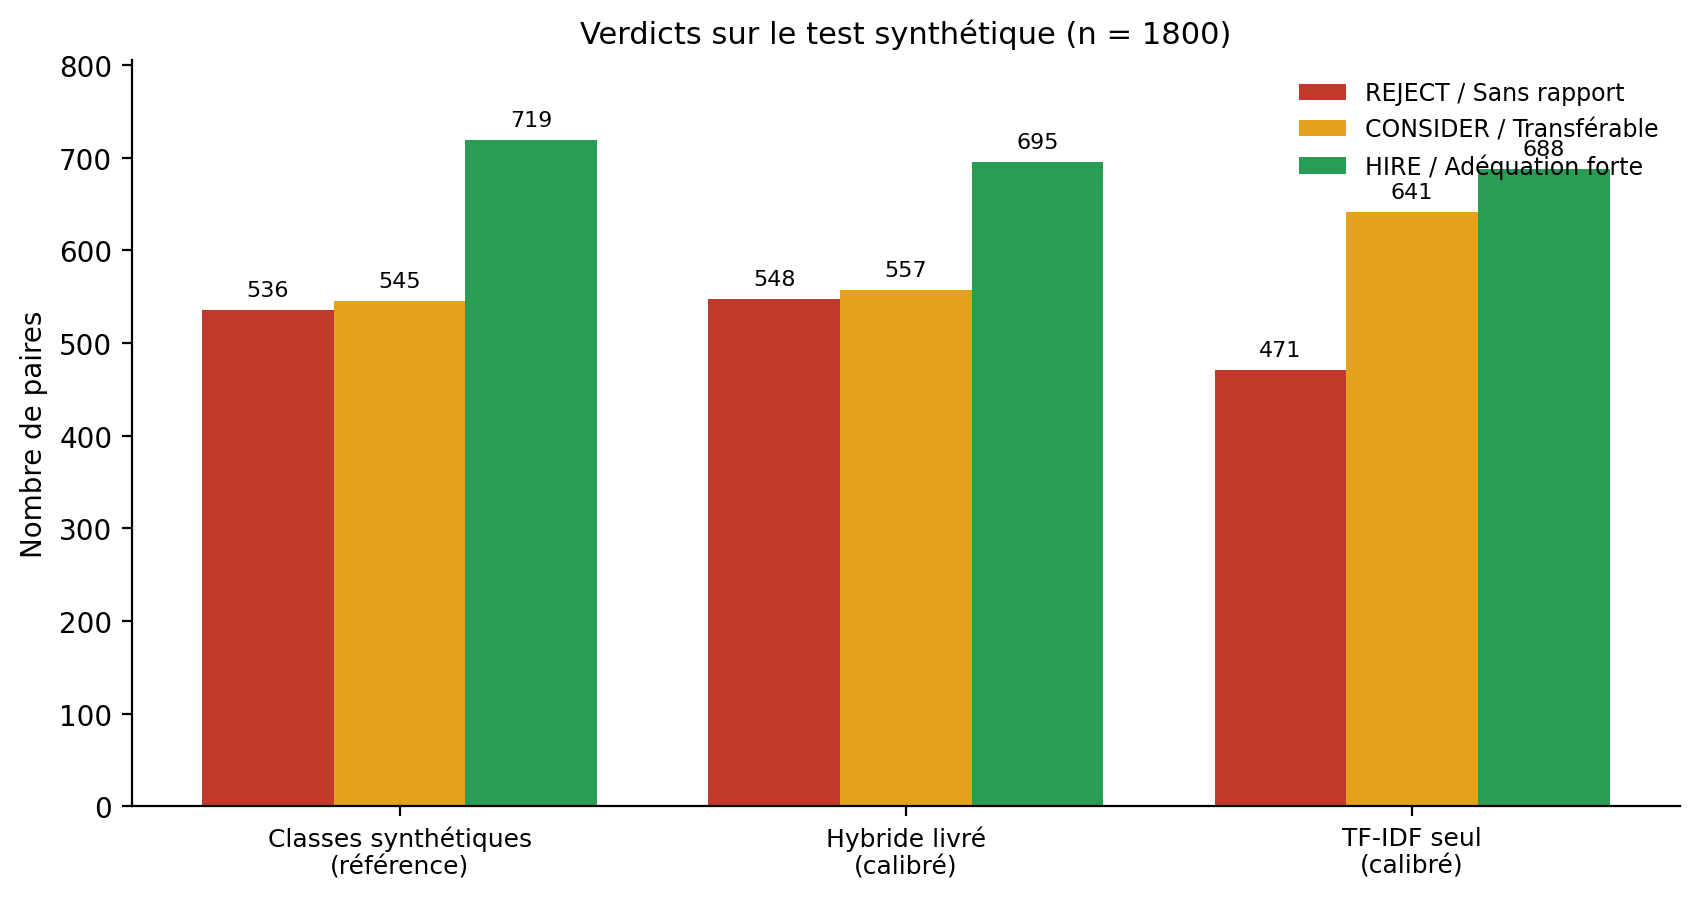
\includegraphics[width=.92\textwidth]{img/ai/eval_verdict_distribution.png}
  \caption{Répartition des verdicts}
  \label{fig:chap4-verdicts-repartition}
\end{figure}

La matrice de confusion de la version finale (figure~\ref{fig:chap4-confusion-verdicts}) montre que les erreurs se concentrent entre classes voisines. Les paires sans rapport sont bien identifiées (459 \texttt{REJECT} sur 536, aucune \texttt{HIRE}), et 553 des 719 adéquations fortes reçoivent \texttt{HIRE}. La classe intermédiaire reste la plus difficile (F1 de 0,59)~: 325 profils transférables sur 545 reçoivent \texttt{CONSIDER}, 142 \texttt{HIRE} et 78 \texttt{REJECT}. Une comparaison appariée par bootstrap sur les mêmes paires ne montre pas de différence entre l'hybride calibré et TF--IDF seul (écart de $-0{,}006$, IC à 95~\% de $-0{,}028$ à $0{,}016$). Les paires multilingues (CV anglais, offre française, 120 paires) sont moins bien traitées que les paires françaises (exactitude de 0,65 contre 0,75).

\begin{figure}[htbp]
  \centering
  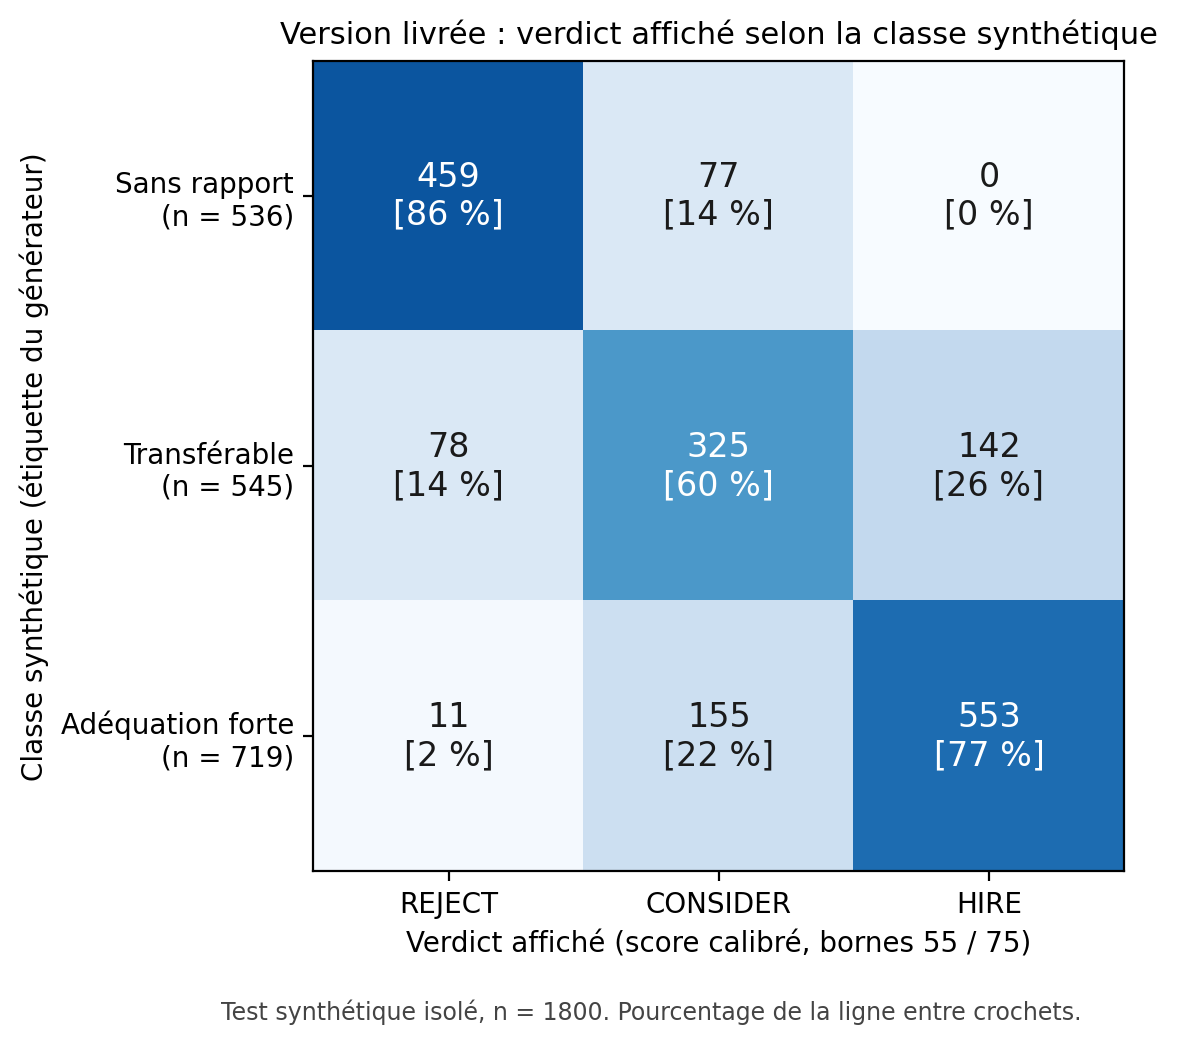
\includegraphics[width=.7\textwidth]{img/ai/eval_confusion_verdicts.png}
  \caption{Matrice de confusion des verdicts}
  \label{fig:chap4-confusion-verdicts}
\end{figure}

\subsection*{Choix de la pondération}
\addcontentsline{toc}{subsection}{Choix de la pondération}

Une fusion dont les poids sont appris sur l'apprentissage seul (0,75 / 0,05 / 0,20) obtient le meilleur macro-F1 en validation comme en test, et la règle de sélection fixée avant la lecture du test la désignait. Elle n'est pas retenue pour le produit, pour deux raisons. D'abord, son avantage provient d'un corpus dont les étiquettes sont construites à partir du recouvrement des compétences recopiées dans l'offre, ce qui favorise mécaniquement le signal lexical. Ensuite, une pondération dominée par TF--IDF récompense la simple reprise du vocabulaire de l'annonce. Sur une paire contrôlée de CV de même substance, l'un calqué sur l'offre et l'autre reformulé, une pondération 0,9 / 0,0 / 0,1 donnait un écart de 25,6 points, contre 9,6 points avec la pondération documentée (Tableau~\ref{tab:chap4-bug4}). La version finale conserve donc la pondération documentée 0,2 / 0,4 / 0,4~; la calibration de la fusion apprise est archivée avec le code.

\begin{table}[H]
  \centering
  \small
  \caption{Effet de la reformulation selon la pondération}
  \label{tab:chap4-bug4}
  \begin{tabular}{|l|r|r|r|}
    \hline
    Pondération du moteur & CV calqué sur l'offre & CV reformulé & Écart \\
    \hline
    0,9 / 0,0 / 0,1 & 99,2 & 73,6 & 25,6 points \\
    \hline
    0,2 / 0,4 / 0,4 (documentée) & 94,4 & 84,8 & 9,6 points \\
    \hline
  \end{tabular}
\end{table}

\subsection*{Robustesse face aux CV manipulés}
\addcontentsline{toc}{subsection}{Robustesse face aux CV manipulés}

Le Tableau~\ref{tab:chap4-robustesse} mesure l'effet du contrôle des preuves sur des CV de la partition de validation modifiés de façon contrôlée, à raison de 200 paires par scénario. Les cinq premiers scénarios partent de profils sans rapport avec l'offre~; les deux derniers partent d'adéquations fortes. Les deux colonnes utilisent la même calibration~; seule change la présence du contrôle des preuves. Je n'ai ajusté aucun paramètre sur ces scénarios.

\begin{table}[htbp]
  \centering
  \footnotesize
  \caption{Effet du contrôle des preuves}
  \label{tab:chap4-robustesse}
  \begin{tabular}{|p{7.2cm}|c|c|}
    \hline
    Scénario & Sans contrôle & Version finale \\
    \hline
    Référence~: profils sans rapport non modifiés & \multicolumn{2}{c|}{174 / 25 / 1} \\
    \hline
    Profil sans rapport + liste d'exigences de l'offre recopiée & 0 / 0 / 200 & 133 / 67 / 0 \\
    \hline
    Profil sans rapport + mêmes compétences, réordonnées, dans une section Compétences & 0 / 0 / 200 & 0 / 200 / 0 \\
    \hline
    Profil sans rapport + offre entière collée & 0 / 0 / 200 & 174 / 26 / 0 \\
    \hline
    Profil sans rapport + mention niée des compétences & 0 / 0 / 200 & 175 / 24 / 1 \\
    \hline
    Profil sans rapport + compétences insérées dans une phrase d'expérience & 0 / 0 / 200 & 0 / 0 / 200 \\
    \hline
    Référence~: adéquations fortes non modifiées & \multicolumn{2}{c|}{1 / 33 / 166} \\
    \hline
    Adéquation forte privée de la moitié de ses compétences & 15 / 129 / 56 & 15 / 129 / 56 \\
    \hline
    Adéquation forte allongée par des expériences sans rapport & 0 / 16 / 184 & 0 / 16 / 184 \\
    \hline
  \end{tabular}
\end{table}

Le contrôle ramène les listes recopiées, l'offre collée et les mentions niées au niveau de la référence non modifiée~: aucun CV à liste recopiée ou à offre collée n'obtient \texttt{HIRE}, et le seul \texttt{HIRE} restant parmi les mentions niées correspond à un profil déjà mal classé avant modification. Une liste réordonnée placée dans une section Compétences n'est pas reconnue comme copie, mais la règle de prudence ramène le verdict à \texttt{CONSIDER}. Les CV partiels et les CV longs ne sont pas affectés, et aucun verdict des 1\,800 paires authentiques de validation ne change. En revanche, un CV qui affirme une expérience dans une phrase rédigée reste classé \texttt{HIRE}~: l'analyse du texte ne peut pas distinguer une déclaration mensongère d'une expérience réelle. Cette limite justifie la lecture humaine du dossier et les questions d'entretien proposées par la couche~2.

Sur le déploiement Azure CPU, un essai de couche~2 a produit les cinq sections attendues en 54\,290,6~ms. Cette mesure ponctuelle décrit la démonstration, non une garantie de latence ou une évaluation de qualité générative.

\section{Limites, risques et perspectives}

Les résultats quantitatifs sont internes à un corpus synthétique et à des étiquettes générées par règles~; les ancrages de calibration sont appris sur ces étiquettes. Les essais que j'ai menés avec mes propres CV face à des offres réelles, présentés au chapitre~\ref{chap:tests-securite}, sont fonctionnels~: faute de jugements de référence établis par des recruteurs, ils ne permettent de calculer ni précision, ni rappel, ni F1. Les mesures ne couvrent ni la qualité d'une embauche, ni les effets sur les candidats, ni l'équité entre groupes protégés. Un CV qui décrit faussement une expérience n'est pas détecté. Le dictionnaire peut omettre une technologie ou mal qualifier un intitulé ambigu~; les embeddings peuvent rapprocher des contenus trop généraux~; le modèle local peut produire une justification plausible mais erronée. JobTest doit donc rester une aide à la priorisation, avec révision humaine, traçabilité des critères et possibilité de correction.

Les suites nécessaires sont une validation avec des recruteurs sur des données autorisées et minimisées, la mesure de l'accord inter-évaluateurs, des tests de biais et de robustesse par sous-groupes, ainsi qu'un réapprentissage des ancrages de calibration sur ces données annotées. L'évaluation du modèle de langage doit être séparée de celle du score~: fidélité aux faits, utilité des questions et taux d'incohérences sont des axes distincts.

Le tableau~\ref{tab:chap4-synthese} récapitule le rôle de chaque couche et le garde-fou qui lui est associé.

\begin{table}[H]
  \centering
  \caption{Synthèse des couches}
  \label{tab:chap4-synthese}
  \begin{tabular}{|p{3cm}|p{4cm}|p{5cm}|}
    \hline
    Couche & Rôle & Statut et garde-fou \\
    \hline
    Couche~1 & score hybride calibré, contrôle des preuves, décision et explications & implémentée~; décision déterministe~; \texttt{HIRE} écarté si les preuves sont insuffisantes \\
\hline
    Couche~2 & analyse locale et questions d'entretien & optionnelle~; ne change jamais la couche~1 \\
\hline
    Évaluation & benchmark train/validation/test synthétique & disponible~; ancrages appris sur étiquettes synthétiques~; non représentatif d'une embauche réelle \\
    \hline
  \end{tabular}
\end{table}

\section*{Conclusion}
\addcontentsline{toc}{section}{Conclusion}

Le moteur combine signaux lexicaux, sémantiques et structurés, contrôle les preuves avant le calcul et calibre son score avant d'appliquer les bandes de décision. Sur le test synthétique, les verdicts affichés atteignent un macro-F1 de 0,740 sur trois classes, sans dépasser TF--IDF seul, et les CV qui recopient l'offre n'obtiennent plus \texttt{HIRE}. La calibration devra être réapprise sur des données réelles annotées avant tout usage opérationnel. Le chapitre suivant présente la réalisation de la plateforme.

        \clearpage
        \chapter{Réalisation et présentation de la plateforme}

\section*{Introduction}

Ce chapitre décrit le passage de la conception à une plateforme utilisable par un recruteur. L'enjeu n'est pas de reprendre l'architecture logique ni les calculs présentés précédemment, mais de montrer comment ils sont rendus accessibles par une application Web cohérente : saisie des données, exécution d'une évaluation, restitution expliquée et conservation des résultats. Les éléments décrits ci-après proviennent de la version courante du dépôt JobTest ; l'ancienne interface Streamlit est donc considérée comme un prototype et non comme l'interface finale.

\section{Environnement matériel et logiciel}

\subsection{Environnement matériel}

J'ai réalisé le développement, les validations locales et la rédaction de ce mémoire sur mon ordinateur personnel, décrit ci-dessous. Cet environnement local est distinct de la machine virtuelle Azure décrite au chapitre~6 ; aucune mesure de performance matérielle n'est déduite de ces caractéristiques.

Le tableau~\ref{tab:chap5-hardware} en donne les caractéristiques.

\begin{table}[H]
\centering
\small
\caption{Environnement matériel}
\label{tab:chap5-hardware}
\begin{tabularx}{.82\textwidth}{|p{.34\textwidth}|X|}
\hline
\textbf{Composant} & \textbf{Caractéristique}\\ \hline
Ordinateur & HP\\ \hline
Processeur & Intel Core i3, 11\textsuperscript{e} génération\\ \hline
Mémoire vive & 8 Go de RAM\\ \hline
Processeur graphique & Intel UHD Graphics\\ \hline
Stockage total & Environ 1 300 Go\\ \hline
\end{tabularx}
\end{table}

\subsection{Environnement logiciel}

Le développement associe un service Python et une application Web Next.js. L'environnement local s'appuie sur Windows, Python, Node.js et \texttt{npm}. L'API est exécutée avec Uvicorn ; le navigateur sert à vérifier les parcours de l'interface. Git est utilisé pour le suivi des sources. Les versions expressément verrouillées par le projet sont indiquées ; aucune version non vérifiable de système, d'éditeur ou de navigateur n'est inférée.

Le tableau~\ref{tab:chap5-environment} récapitule ces outils et le rôle tenu par chacun.

\begin{table}[H]
\centering
\small
\caption{Environnement de réalisation}
\label{tab:chap5-environment}
\begin{tabularx}{\textwidth}{|l|l|X|}
\hline
\textbf{Élément} & \textbf{Outil ou technologie} & \textbf{Rôle dans le projet}\\
\hline
Système local & Windows & Développement et exécution locale des services.\\
\hline
Backend & Python, FastAPI et Uvicorn & Exposition de l'API, services métier et exécution ASGI.\\
\hline
Frontend & Next.js 14.2.35, React 18, TypeScript & Pages App Router, composants et interactions du recruteur.\\
\hline
Styles et animation & Tailwind CSS, Framer Motion & Système visuel, états de l'interface et transitions.\\
\hline
Données locales & SQLite et SQLAlchemy & Persistance locale des comptes, offres, candidats, CV et évaluations.\\
\hline
Outils IA & scikit-learn, Sentence-Transformers, spaCy, Ollama & Moteur de rapprochement et analyse qualitative optionnelle.\\
\hline
Documents & ReportLab & Construction du rapport PDF d'évaluation.\\
\hline
Conteneurs & Docker Compose, Caddy, PostgreSQL & Environnement de déploiement ; détaillé au chapitre 6.\\
\hline
\end{tabularx}
\end{table}

\section{Choix des technologies}

Les choix présentés dans cette section sont justifiés par les responsabilités effectivement portées par chaque partie de JobTest.

\subsection{Technologies frontend}

Le répertoire \texttt{web/} contient le frontend final. Next.js organise les écrans dans \texttt{app/}, selon l'App Router, et React porte les composants réutilisables. TypeScript définit les contrats manipulés par le client API et évite que les données de réponse soient traitées comme des objets non structurés. Les routes principales correspondent notamment à la connexion, à la vue d'ensemble, aux offres, aux candidats, à l'analyse, à l'historique, au classement et au centre de qualité.

Tailwind CSS est employé pour composer les styles de l'interface et les variantes des composants communs, tels que boutons, cartes, tableaux, badges, champs et états vides. Framer Motion est utilisé pour les transitions de pages, l'apparition du résultat et les animations de score. Le projet référence également Three.js, \texttt{@react-three/fiber} et \texttt{@react-three/drei} ; leur emploi est concret dans les éléments graphiques \texttt{AmbientBackground}, \texttt{ScoreTorus} et \texttt{NeuralField}. Ces éléments complètent la lecture visuelle du score sans porter la décision elle-même.

\subsection{Technologies backend}

FastAPI regroupe l'API sous le préfixe \texttt{/api/v1}. L'application installe les routeurs d'authentification et le routeur \texttt{/api/v1/ui}, destiné aux besoins du frontend actuel. Les modèles Pydantic définissent et valident les corps des requêtes, par exemple une offre, une évaluation ou une demande de rapport. La séparation rend explicites les entrées HTTP avant l'appel aux services de rapprochement.

SQLAlchemy représente les entités \emph{User}, \emph{Candidate}, \emph{CV}, \emph{JobOffer}, \emph{MatchResult} et \emph{Skill}. Les relations lient le candidat à ses CV et ses résultats, et le recruteur à ses propres candidats et offres. Les contrôles de propriété appliqués par l'API empêchent qu'un identifiant d'offre ou de candidat appartenant à un autre recruteur soit utilisé dans une évaluation.

Le parsing des CV repose sur \texttt{pdfplumber} avec repli \texttt{PyPDF2} pour les PDF, et sur \texttt{python-docx} avec repli XML pour les documents Word. ReportLab génère le PDF à partir des données déjà calculées : en-tête, identité affichée, score, radar, compétences, écarts, recommandations et aide à la décision. La génération reste ainsi découplée de l'affichage Next.js.

L'authentification s'appuie sur des jetons JWT transmis dans l'en-tête \texttt{Authorization: Bearer}. Le client conserve le jeton dans le stockage local du navigateur et l'ajoute aux appels protégés. Les mots de passe ne sont pas retournés par les endpoints ; seul le hachage est conservé dans le modèle utilisateur.

\subsection{Technologies d'intelligence artificielle}

Le premier niveau d'analyse mobilise les composants décrits au chapitre~\ref{chap:moteur-intelligent} : TF--IDF de scikit-learn, similarité sémantique avec Sentence-Transformers, extraction et rapprochement de compétences, puis fusion hybride. spaCy intervient lorsqu'un modèle linguistique est disponible, avec une stratégie de repli dans le prétraitement. Le chargement des services est différé jusqu'à la première requête nécessitant le moteur, ce qui permet à l'API de démarrer sans calculer immédiatement les modèles.

La seconde couche qualitative est appelée après l'affichage du résultat principal. Le runtime local Ollama est configuré avec \texttt{qwen2.5:1.5b}. Son indisponibilité n'empêche pas l'évaluation statistique : la réponse expose alors un état contrôlé tel que \emph{unavailable}, \emph{disabled} ou \emph{error}. Cette distinction est importante pour l'utilisateur : l'analyse approfondie enrichit la lecture, mais ne modifie ni le score ni le verdict du premier niveau.

\subsection{Technologies de données et d'infrastructure}

SQLite constitue le choix par défaut en développement local grâce à une base fichier et à l'intégration SQLAlchemy. Pour l'environnement conteneurisé, le fichier \texttt{docker-compose.yml} définit PostgreSQL 16 comme service de données. Docker Compose réunit également l'API, l'application Web, Ollama et le proxy inverse. Dans la version déployée, ce proxy est Caddy, point d'entrée HTTPS ; il relaie les chemins \texttt{/api/v1/} vers FastAPI et les autres chemins vers Next.js. La procédure complète de sécurisation, de conteneurisation et de déploiement sur machine virtuelle Azure est réservée au chapitre 6.

Le tableau~\ref{tab:chap5-technology-summary} synthétise ces choix et l'usage qui en est réellement fait.

\begin{table}[H]
\centering
\small
\caption{Choix techniques}
\label{tab:chap5-technology-summary}
\begin{tabularx}{\textwidth}{|l|l|X|}
\hline
\textbf{Domaine} & \textbf{Technologie} & \textbf{Utilisation réelle dans JobTest}\\
\hline
Interface & Next.js, React, TypeScript & Écrans App Router, composants et client HTTP.\\
\hline
Présentation & Tailwind CSS, Framer Motion, Three.js & Styles, transitions et représentations visuelles du score.\\
\hline
API & FastAPI, Pydantic & Endpoints, validation et sérialisation JSON.\\
\hline
Persistance & SQLAlchemy, SQLite / PostgreSQL & Entités métier et stockage selon l'environnement.\\
\hline
Rapprochement & scikit-learn, Sentence-Transformers, spaCy & Signaux lexical, sémantique et compétences.\\
\hline
Analyse qualitative & Ollama, Qwen & Analyse approfondie non bloquante.\\
\hline
Export & ReportLab & Rapport PDF téléchargeable.\\
\hline
\end{tabularx}
\end{table}

\section{Organisation du code source}

L'organisation privilégie la séparation entre interface, API, règles de rapprochement et accès aux données. L'arborescence simplifiée suivante ne montre que les dossiers participant directement au fonctionnement de la version étudiée.

\begin{verbatim}
web/                 pages Next.js, composants, client API et styles
src/api/             application FastAPI et routeurs auth / UI
src/matching/        service d'évaluation et persistance du résultat
src/models/          TF-IDF, embeddings, compétences et chargement
src/fusion/          score hybride
src/decisioning/     règles de verdict
src/explainability/  explication et recommandations structurées
src/ai/              prompts et analyse qualitative Ollama
src/parsing/         extraction PDF/DOCX et nettoyage
src/reporting/       génération ReportLab
src/models_db.py     modèles SQLAlchemy
deploy/Caddyfile     proxy inverse HTTPS
\end{verbatim}

Le frontend ne recopie pas les règles du moteur. Son fichier \texttt{lib/api/client.ts} centralise les appels HTTP et les types associés. Côté API, le routeur de parité UI traduit les requêtes de l'interface vers le même service métier que les endpoints techniques. Cette organisation limite les divergences entre un calcul réalisé depuis un écran et un calcul réalisé par API.

\section{Réalisation du backend}

L'initialisation FastAPI crée les tables lorsqu'elles sont absentes et applique une vérification additive de schéma. Les routeurs couvrent l'inscription, la connexion, la lecture de l'utilisateur courant, les offres, les candidats, les résultats, l'évaluation, l'analyse approfondie, la comparaison des modèles, les indicateurs et le rapport PDF. Un middleware ajoute un identifiant de requête, mesure le temps de traitement et applique une limitation de fréquence en mémoire.

Le routeur UI fournit les opérations nécessaires aux pages : lecture et création d'offres, modification de leur statut, consultation et modification des candidats, lecture d'historique, évaluation textuelle ou par fichier, et lecture des indicateurs. Lors d'une évaluation, l'API vérifie l'offre sélectionnée, le contenu minimal du CV et l'appartenance des données au recruteur connecté. Le service \texttt{evaluate\_and\_persist} calcule le résultat, crée ou retrouve le candidat selon les données fournies, conserve le CV et enregistre les sous-scores, le verdict, les seuils actifs et l'explication JSON.

La route de rapport reçoit les objets déjà calculés et renvoie un flux \texttt{application/pdf} avec un en-tête de téléchargement. Ce choix évite de recalculer le matching lors de l'export. De manière analogue, la route d'analyse approfondie reçoit l'identifiant d'un résultat persistant, reconstruit son contexte et renvoie une enveloppe d'état sans faire échouer le parcours lorsque le LLM n'est pas accessible.

\section{Réalisation du frontend}

La zone authentifiée est enveloppée par un layout commun : barre latérale, barre supérieure, transition de page et zone centrale. Au chargement, le layout vérifie la présence du jeton puis appelle \texttt{/auth/me}. En cas d'échec, il redirige vers la connexion. Cette vérification protège l'expérience utilisateur au niveau de l'interface, tandis que l'API vérifie de nouveau le jeton pour chaque ressource protégée.

Les pages utilisent des composants génériques pour maintenir une restitution homogène. \texttt{Table} porte les listes, \texttt{Modal} les opérations de modification ou de confirmation, \texttt{Field} les saisies, et \texttt{DataStates} les états de chargement ou d'absence de données. Les pages d'offres et de candidats affichent leurs données sous forme de tableau et appellent le client centralisé pour actualiser leur état après une modification. Les erreurs réseau ou fonctionnelles sont converties en notifications visibles ; le bouton de l'évaluation affiche également un état de travail pendant le calcul.

La page d'analyse regroupe la sélection d'une offre ouverte, le choix de méthode, l'identité facultative du candidat et deux modes d'entrée du CV : collage de texte ou téléversement PDF/DOCX. Après la réponse JSON, elle révèle le score, le verdict, les composantes, le radar de compétences, les forces, lacunes et recommandations. L'export PDF transmet les données du résultat vers le backend. Le composant \texttt{DeepAnalysis} déclenche séparément la couche qualitative et présente son état sans masquer la restitution du premier niveau.

\section{Intégration frontend--backend}

Le parcours d'une évaluation relie deux responsabilités complémentaires. Le navigateur assure la collecte et la restitution ; le serveur possède les règles métier et les données persistantes.

\begin{enumerate}
  \item Le recruteur choisit une offre et saisit ou téléverse le CV dans l'écran \emph{Candidate Analysis}.
  \item Le frontend contrôle les informations requises et construit une requête vers \texttt{/api/v1/ui/evaluate} ou \texttt{/api/v1/ui/evaluate/file}.
  \item Le client API ajoute le jeton bearer, puis FastAPI valide le schéma Pydantic, l'utilisateur et la propriété de l'offre.
  \item Le service métier extrait éventuellement le document, exécute le moteur de niveau 1 et produit explication, recommandations et décision.
  \item SQLAlchemy conserve le candidat, le CV et le résultat lorsque le parcours est persistant.
  \item La réponse JSON est affichée par les composants de score ; l'analyse approfondie est demandée indépendamment après cette réponse.
  \item Sur demande, le frontend envoie les éléments nécessaires à \texttt{/api/v1/report/pdf} et télécharge le document retourné.
\end{enumerate}

En développement, le client pointe vers l'API locale configurée par \texttt{NEXT\_PUBLIC\_API\_BASE}. Dans le déploiement, le même chemin relatif \texttt{/api/v1} est servi derrière le proxy inverse, ce qui évite d'exposer au navigateur les adresses internes des conteneurs. Les réponses d'erreur HTTP sont transformées en messages d'interface ; l'état particulier de la Layer 2 est, lui, affiché comme une disponibilité de service et non comme un échec de l'évaluation principale.

\section{Présentation des interfaces}

J'ai réalisé les captures de cette section sur une instance locale exécutant la version finale du code (modèle \texttt{hybrid-checkpoint-v4} et calibration versionnée livrée). Je les ai produites avec le navigateur Chrome, piloté par un script du dépôt (\texttt{scripts/capture\_screens.py}), dans une fenêtre de 1\,440 $\times$ 900 pixels, sans autre retouche que le masquage des dates. Pour la lisibilité, la barre de navigation latérale, identique sur toutes les pages et visible sur la figure~\ref{fig:chap5-overview}, est recadrée sur les autres écrans de l'application. Le jeu de démonstration est entièrement fictif~: compte recruteur de test, offres rédigées pour l'occasion, candidats dotés d'adresses \texttt{example.com} et dix-huit CV fictifs au format PDF. Aucun CV personnel n'y figure.

\subsection{Connexion et identité visuelle}

La page de connexion comporte les champs courriel et mot de passe, un lien de création de compte et une notification d'erreur en cas d'échec. Les champs sont vides à l'ouverture. La partie visuelle présente l'identité JobTest et le rôle d'aide au recrutement. Après authentification, l'utilisateur est dirigé vers la vue d'ensemble (figure~\ref{fig:chap5-login}).

\begin{figure}[H]
  \centering
  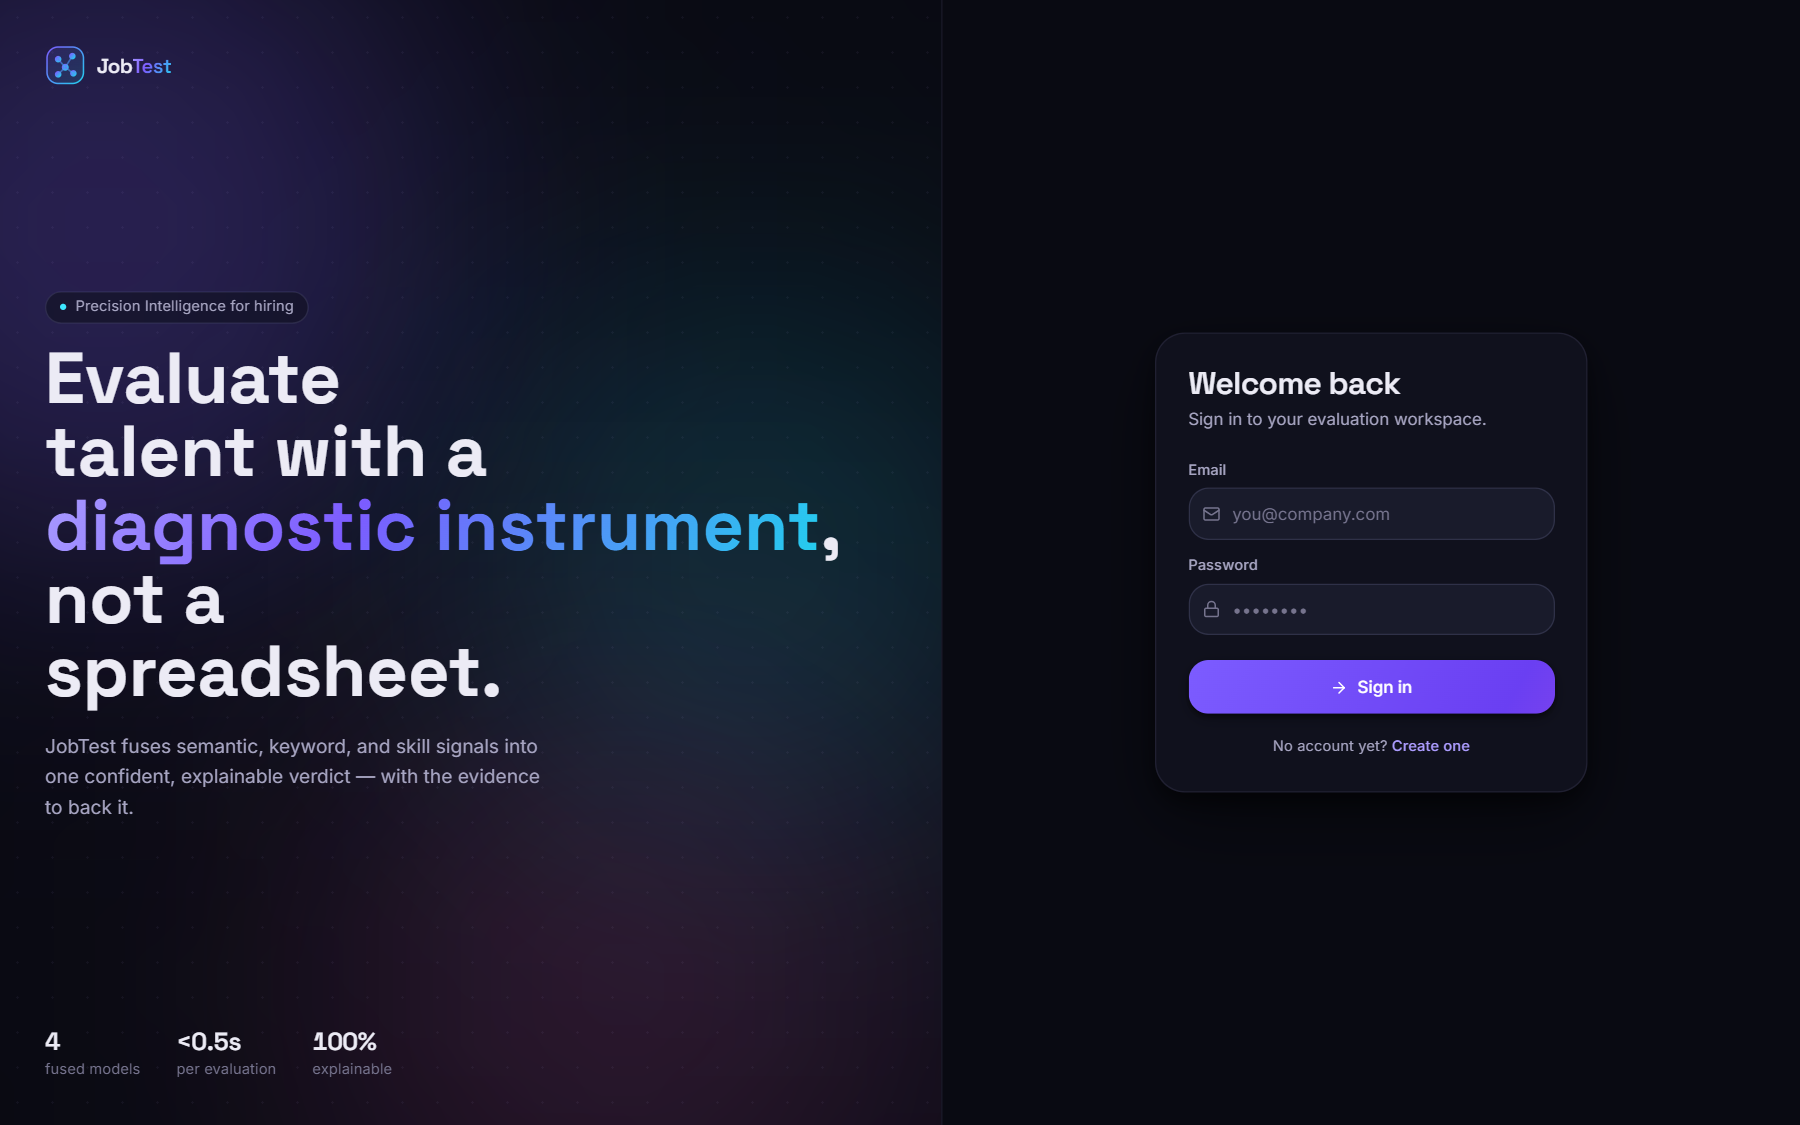
\includegraphics[width=.95\textwidth]{img/interfaces/login.png}
  \caption{Écran de connexion}
  \label{fig:chap5-login}
\end{figure}

L'inscription est proposée sur ce même écran~; elle demande le nom, le courriel, le mot de passe et sa confirmation (figure~\ref{fig:chap5-register}).

\begin{figure}[H]
  \centering
  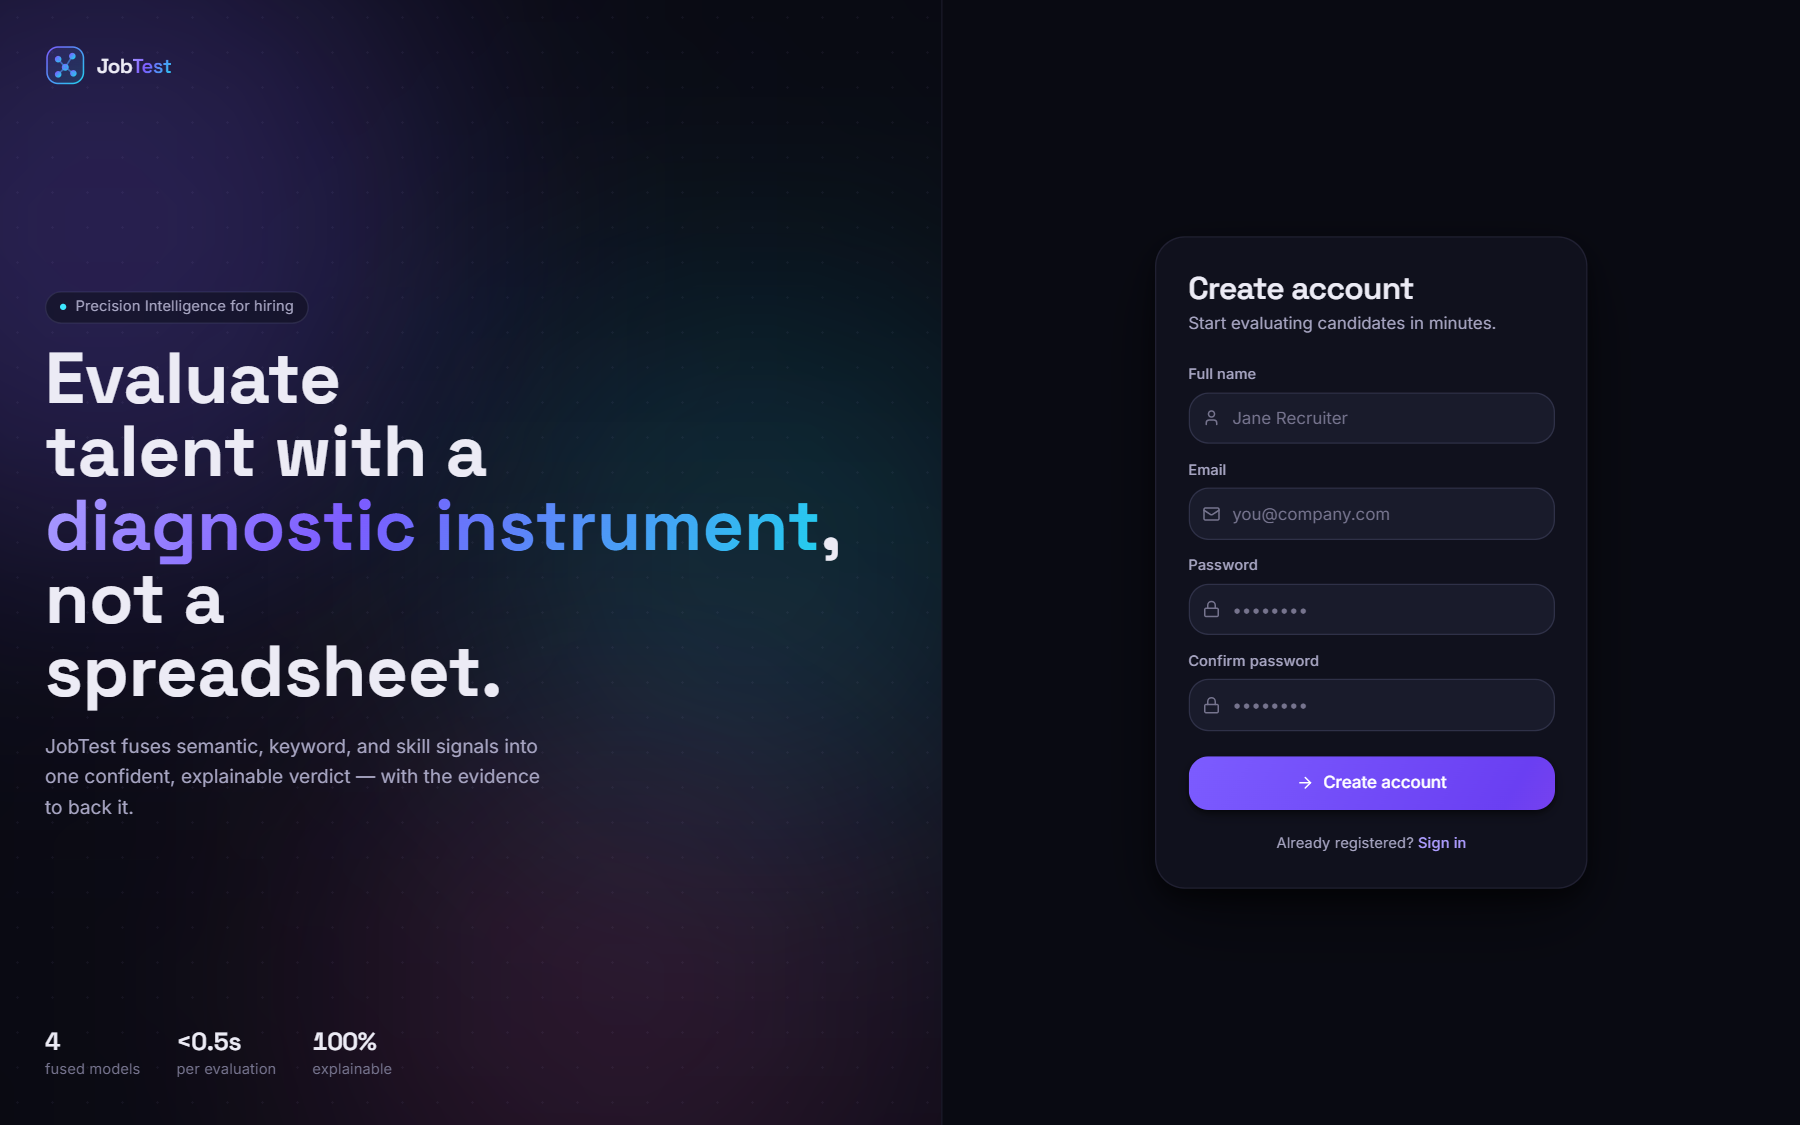
\includegraphics[width=.95\textwidth]{img/interfaces/register.png}
  \caption{Écran d'inscription}
  \label{fig:chap5-register}
\end{figure}

\subsection{Consultation sur mobile}

La mise en page s'adapte aux écrans étroits~: la barre latérale laisse place à une navigation horizontale et les grilles passent sur une colonne, sans modifier les règles métier ni les résultats fournis par l'API. La figure~\ref{fig:chap5-mobile-1} montre la vue d'ensemble et l'historique à la largeur d'un téléphone, obtenus par l'émulation mobile du navigateur (390 pixels de large).

\begin{figure}[H]
  \centering
  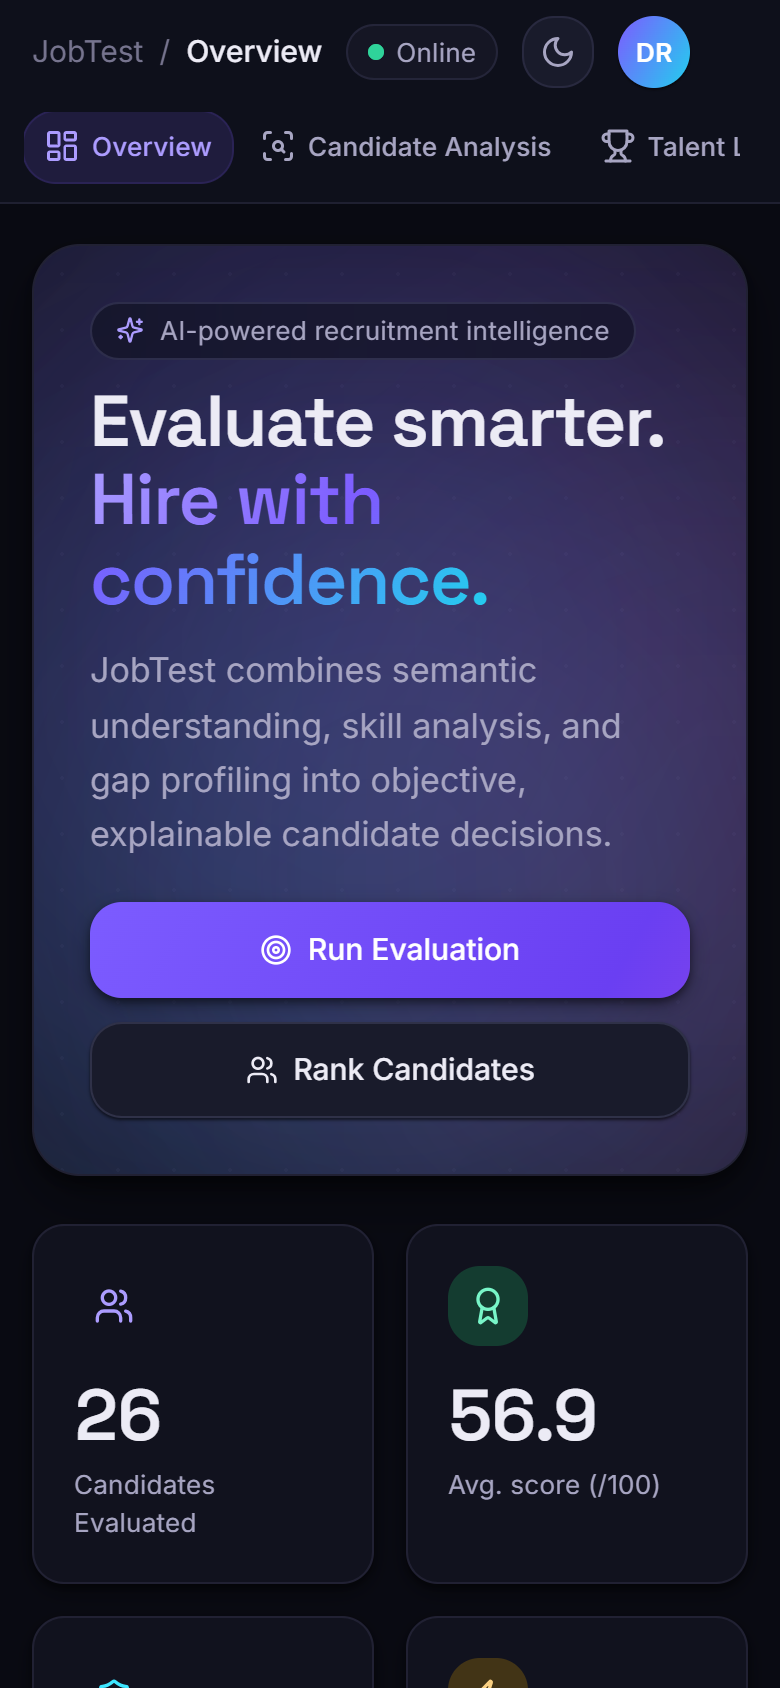
\includegraphics[width=.34\textwidth]{img/interfaces/phone_1.png}\hspace{1.2cm}%
  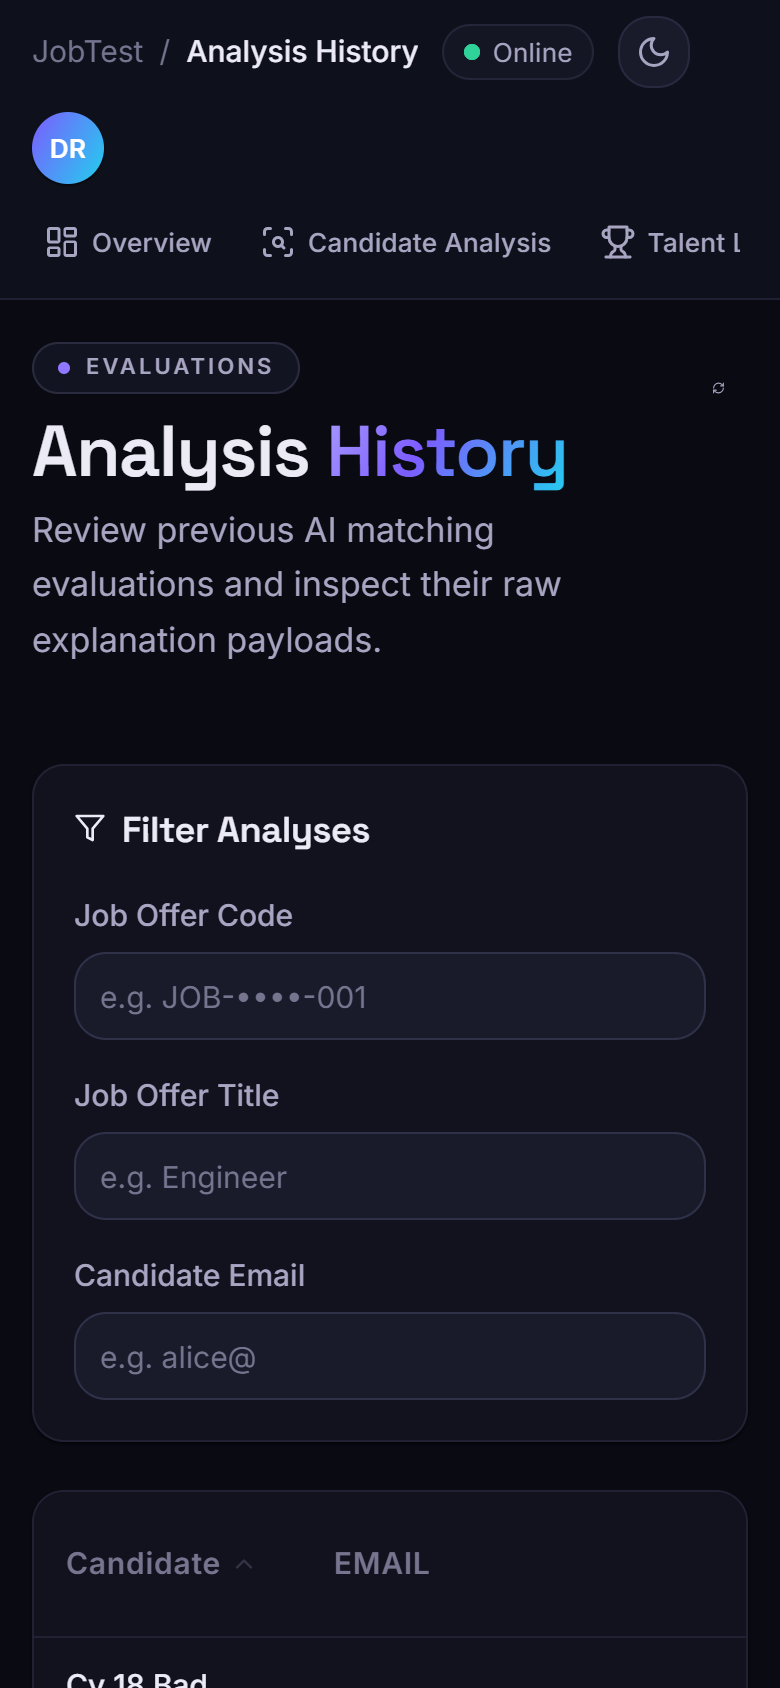
\includegraphics[width=.34\textwidth]{img/interfaces/phone_2.png}
  \caption{Affichage en largeur mobile}
  \label{fig:chap5-mobile-1}
\end{figure}

\subsection{Vue d'ensemble, offres et candidats}

La vue \emph{Overview} synthétise le nombre de candidats, le nombre d'offres, le nombre d'évaluations, le score calibré moyen sur 100 ainsi que la part des verdicts \texttt{HIRE}, puis les résultats récents et la répartition des verdicts. Ces valeurs sont calculées côté API à partir des objets appartenant au recruteur connecté, et seuls les résultats calculés sur l'échelle calibrée entrent dans les moyennes (figure~\ref{fig:chap5-overview}).

\begin{figure}[H]
  \centering
  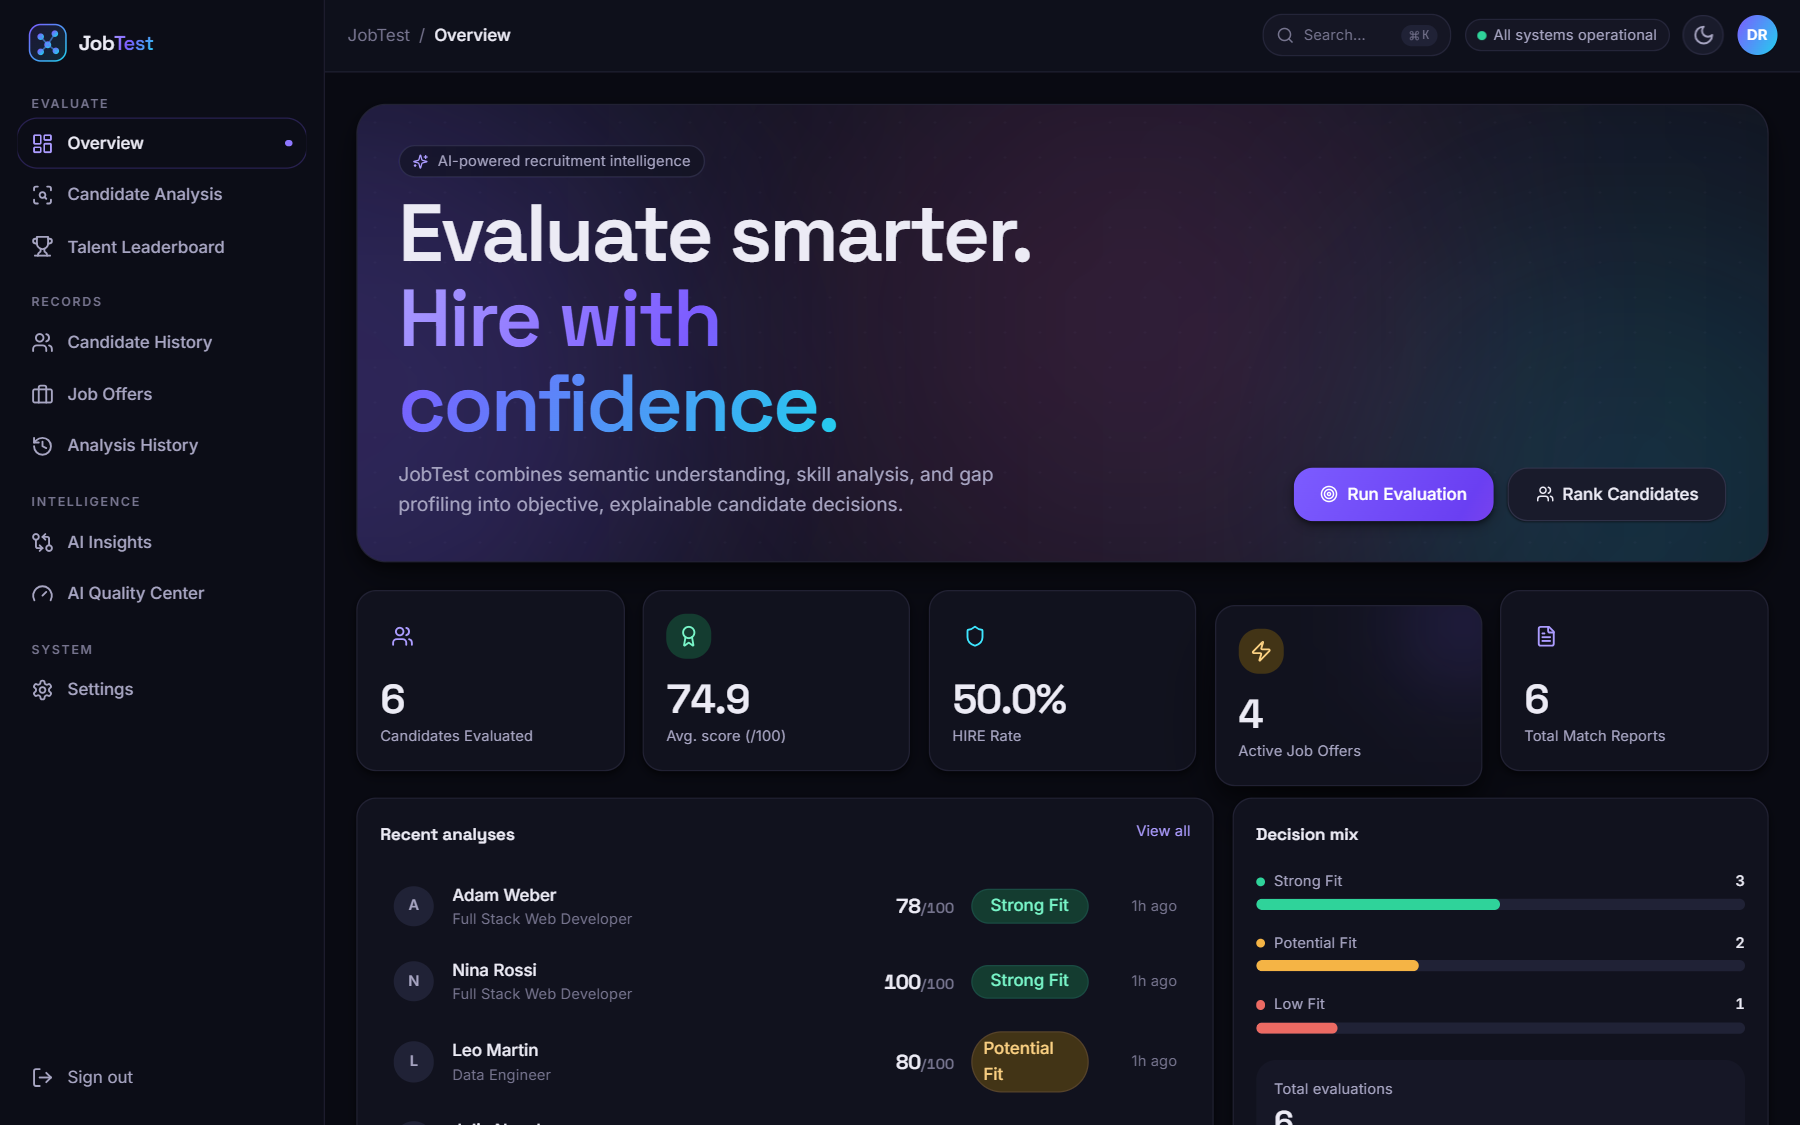
\includegraphics[width=.95\textwidth]{img/interfaces/overview.png}
  \caption{Vue d'ensemble}
  \label{fig:chap5-overview}
\end{figure}

La figure~\ref{fig:chap5-search} illustre la recherche transversale accessible depuis la barre supérieure (raccourci \texttt{Ctrl+K}).

\begin{figure}[H]
  \centering
  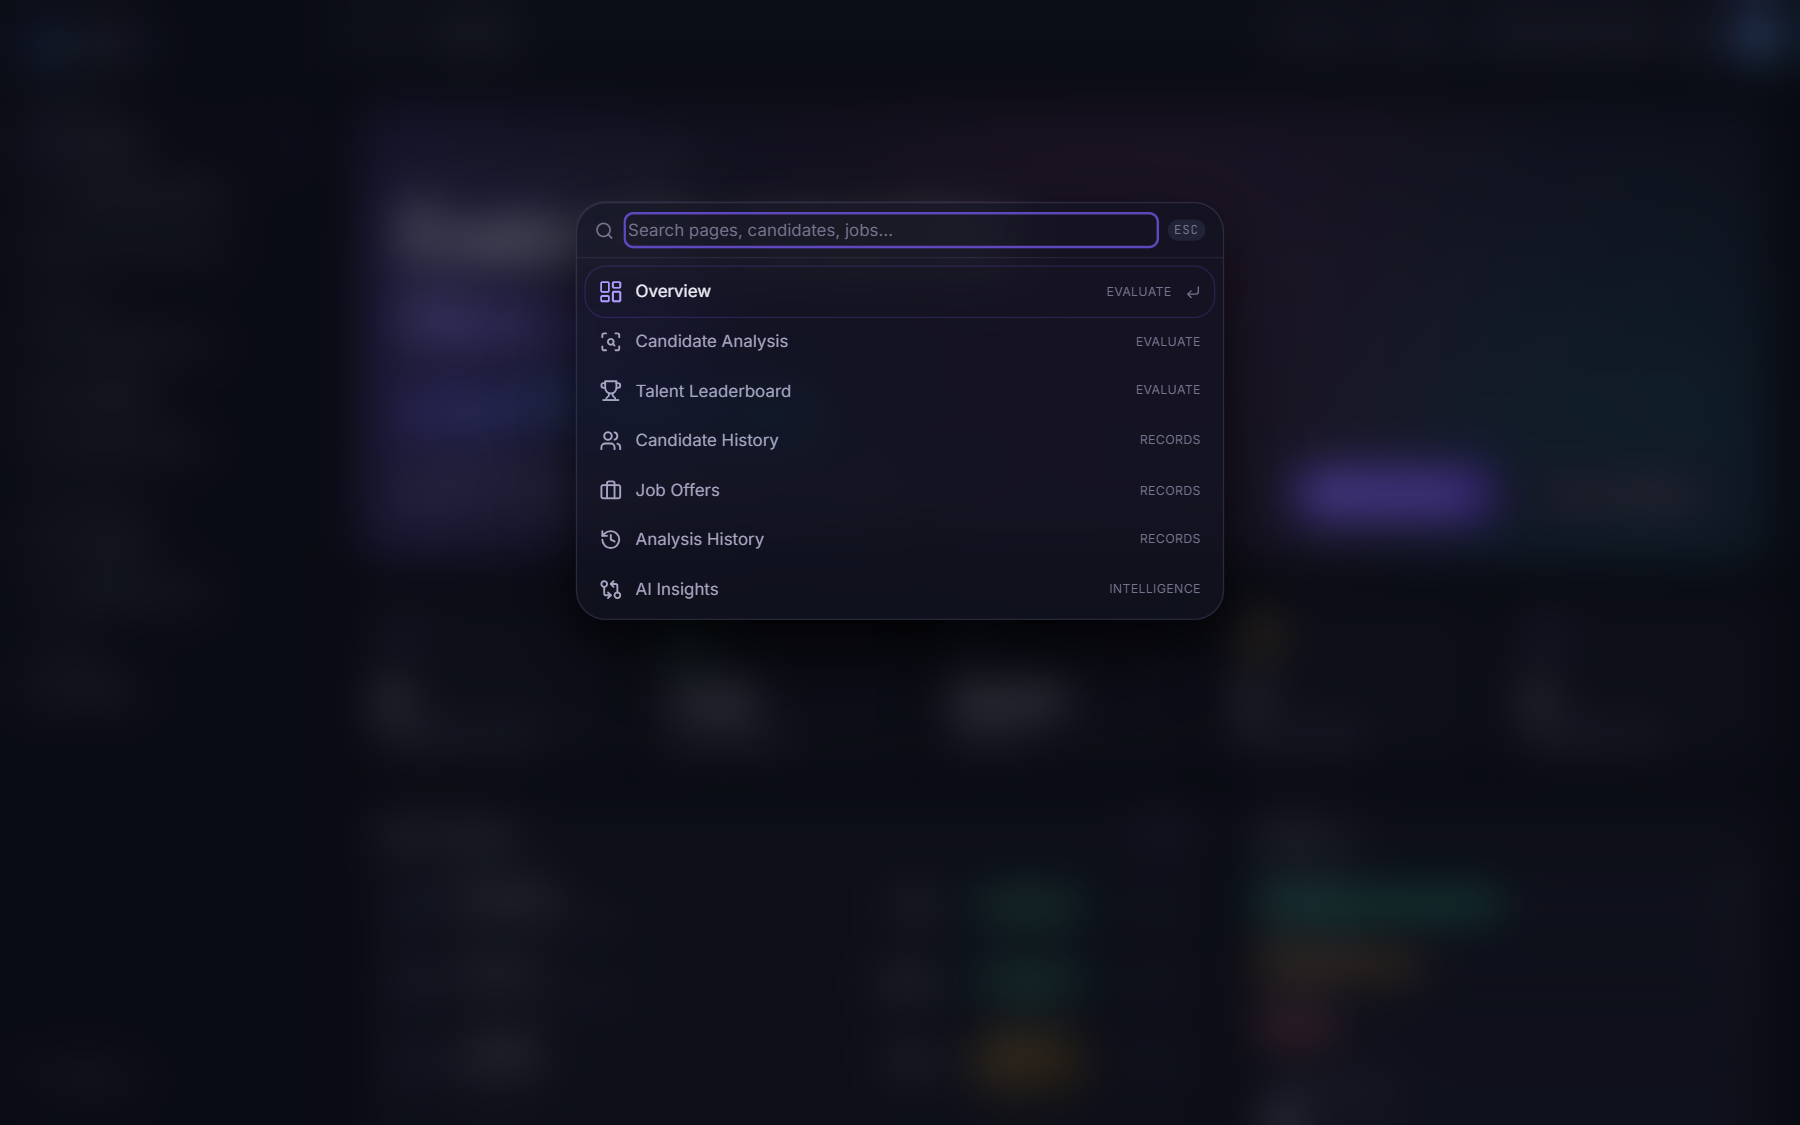
\includegraphics[width=.95\textwidth]{img/interfaces/search.png}
  \caption{Recherche transversale}
  \label{fig:chap5-search}
\end{figure}

La page \emph{Job Offers} permet de créer, consulter, modifier, fermer ou rouvrir une offre. Chaque offre possède un code, un titre, une description, des compétences demandées et un statut parmi \emph{OPEN}, \emph{ON\_HOLD} et \emph{CLOSED} (figures~\ref{fig:chap5-job-offers} et~\ref{fig:chap5-add-job-offer}).

\begin{figure}[H]
  \centering
  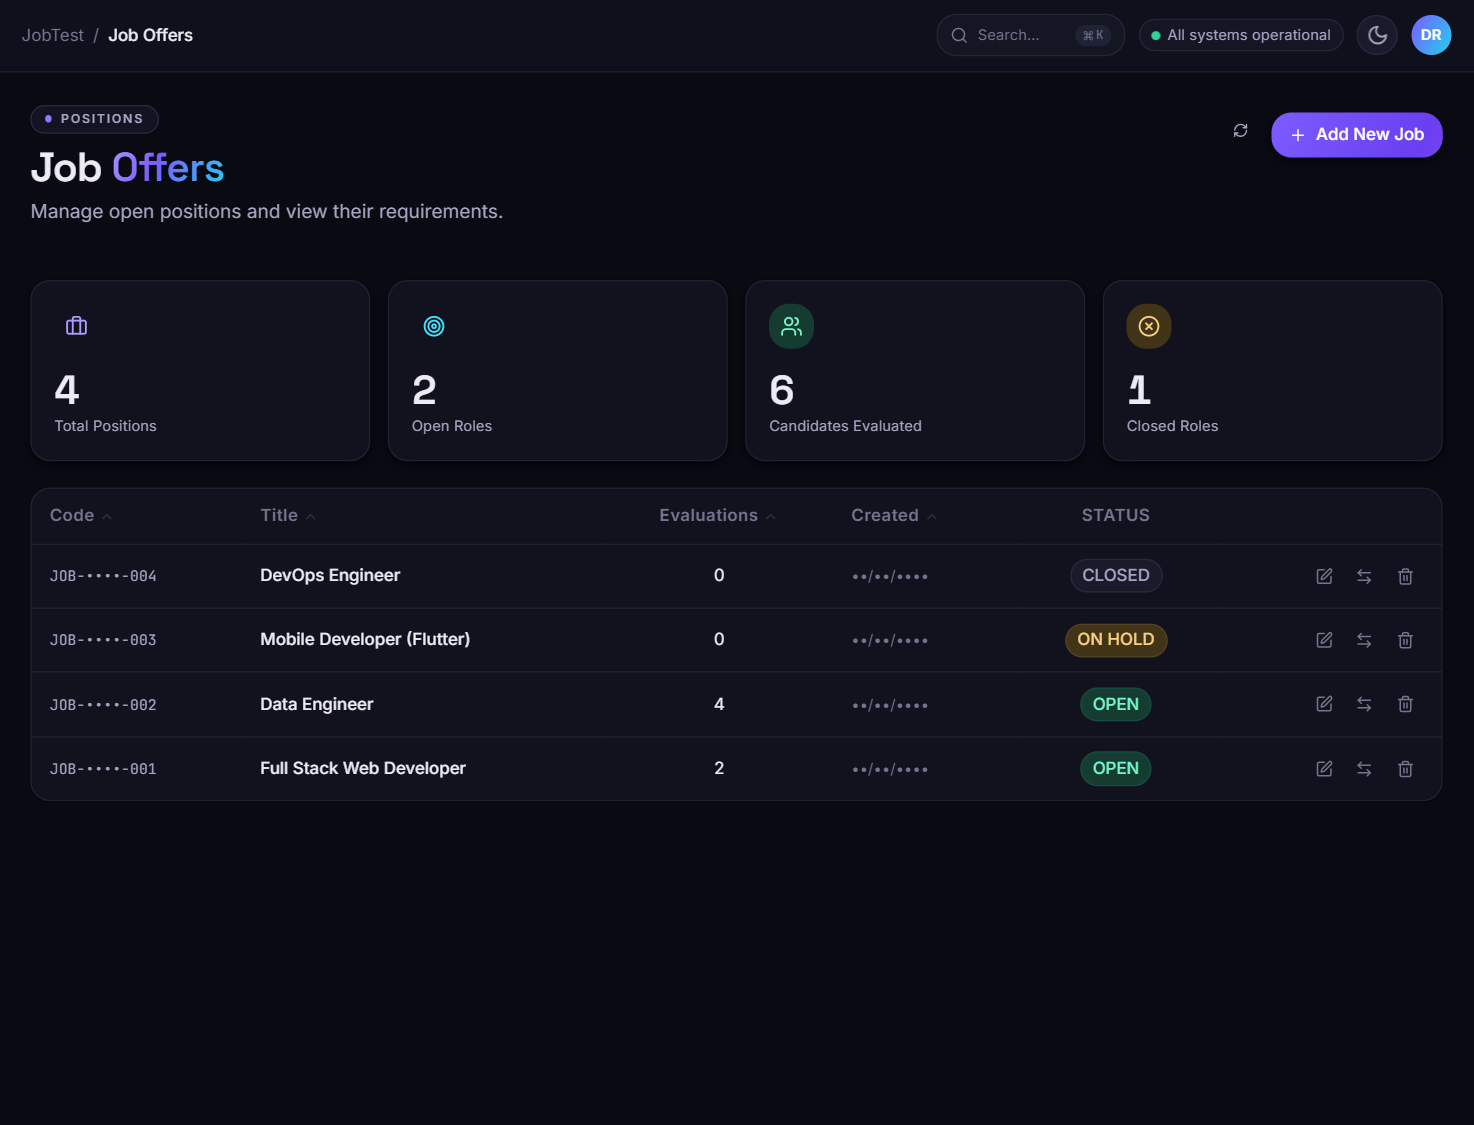
\includegraphics[width=.8\textwidth]{img/interfaces/job_offers.png}
  \caption{Liste des offres d'emploi}
  \label{fig:chap5-job-offers}
\end{figure}

\begin{figure}[H]
  \centering
  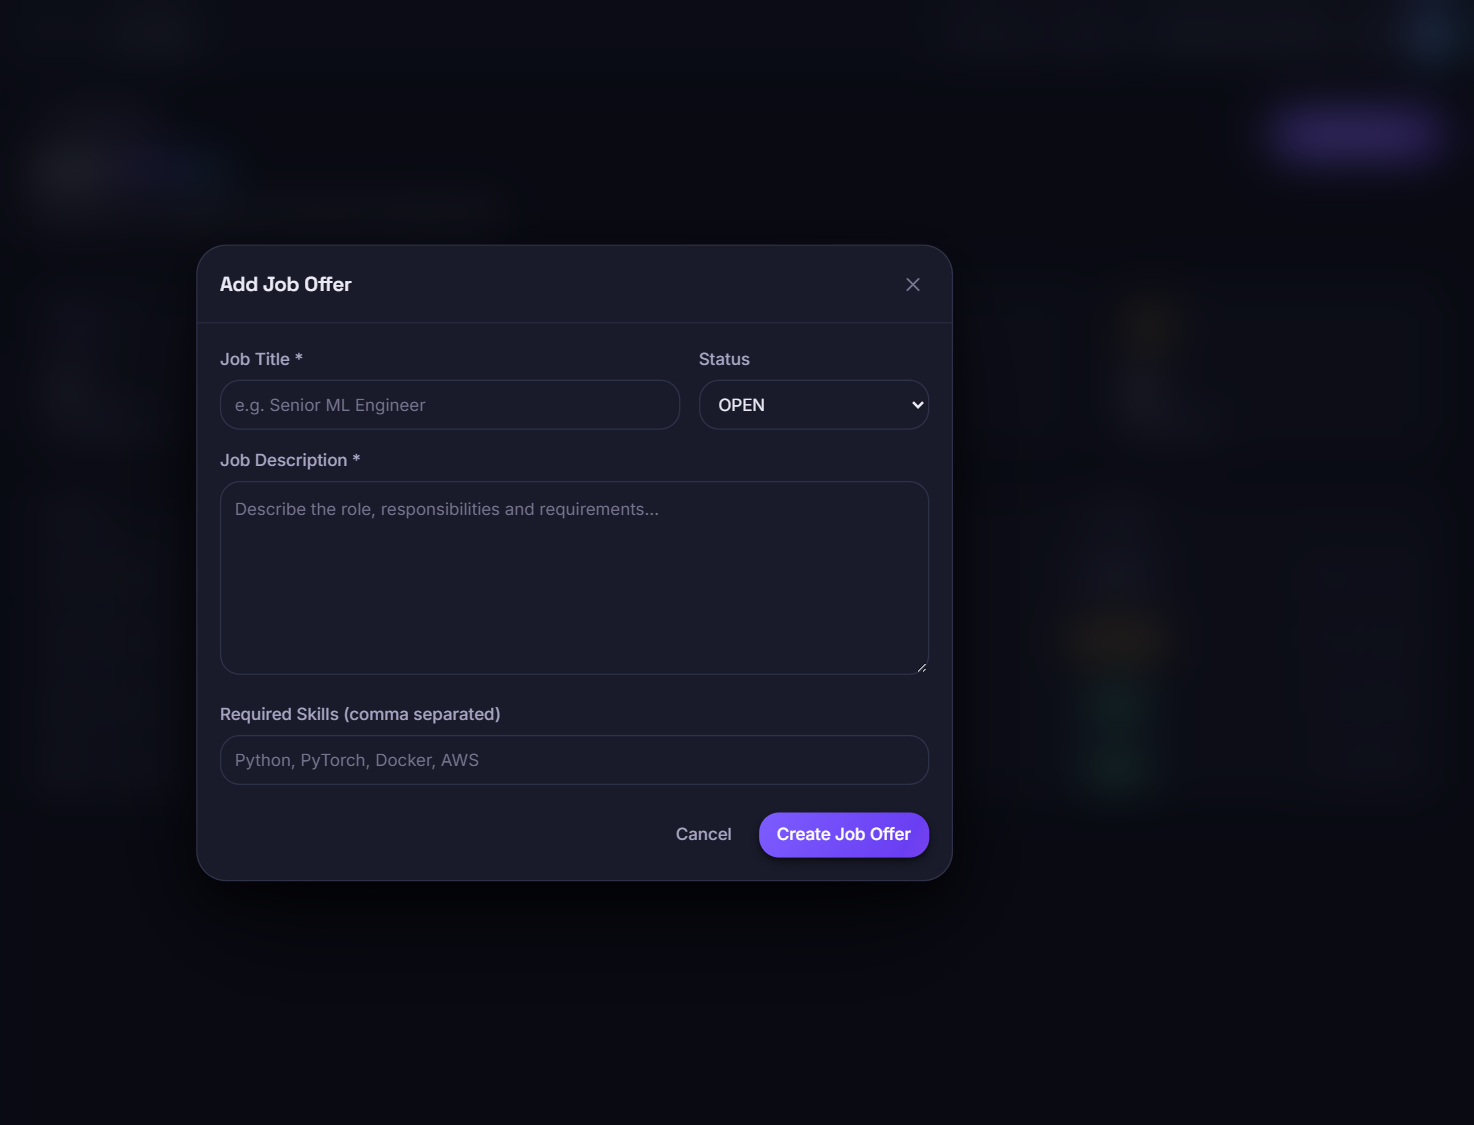
\includegraphics[width=.8\textwidth]{img/interfaces/add_job_offer.png}
  \caption{Création d'une offre d'emploi}
  \label{fig:chap5-add-job-offer}
\end{figure}

La page \emph{Candidate History} distingue les candidats des comptes recruteurs. Elle affiche les informations disponibles, l'état du parcours, le nombre d'évaluations et le meilleur score calibré de chaque candidat~; la modification et la suppression sont des actions explicites (figure~\ref{fig:chap5-candidate-history}).

\begin{figure}[H]
  \centering
  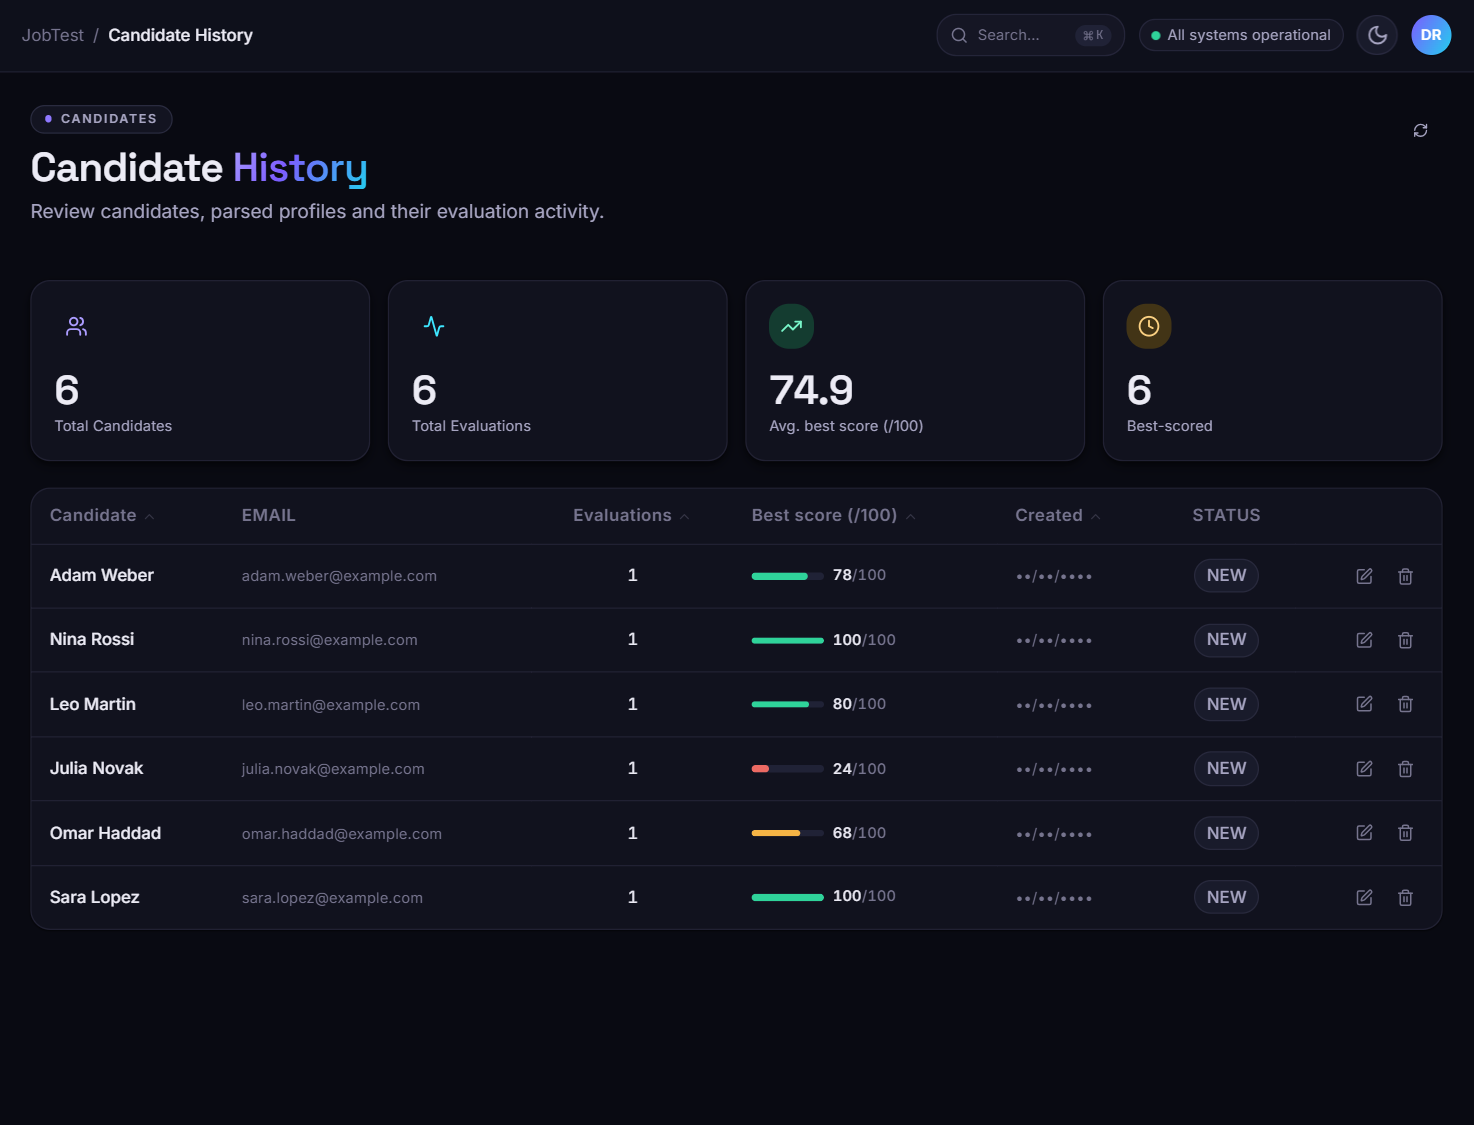
\includegraphics[width=.8\textwidth]{img/interfaces/condidate_history.png}
  \caption{Suivi des candidats}
  \label{fig:chap5-candidate-history}
\end{figure}

L'historique des évaluations liste chaque résultat persisté avec son offre, son score sur 100 et son verdict. Le panneau de détail rappelle la version de calibration, le score brut de la méthode et les seuils appliqués lors du calcul~; un résultat calculé sur l'ancienne échelle y serait signalé comme tel (figure~\ref{fig:chap5-analysis-history}).

\begin{figure}[H]
  \centering
  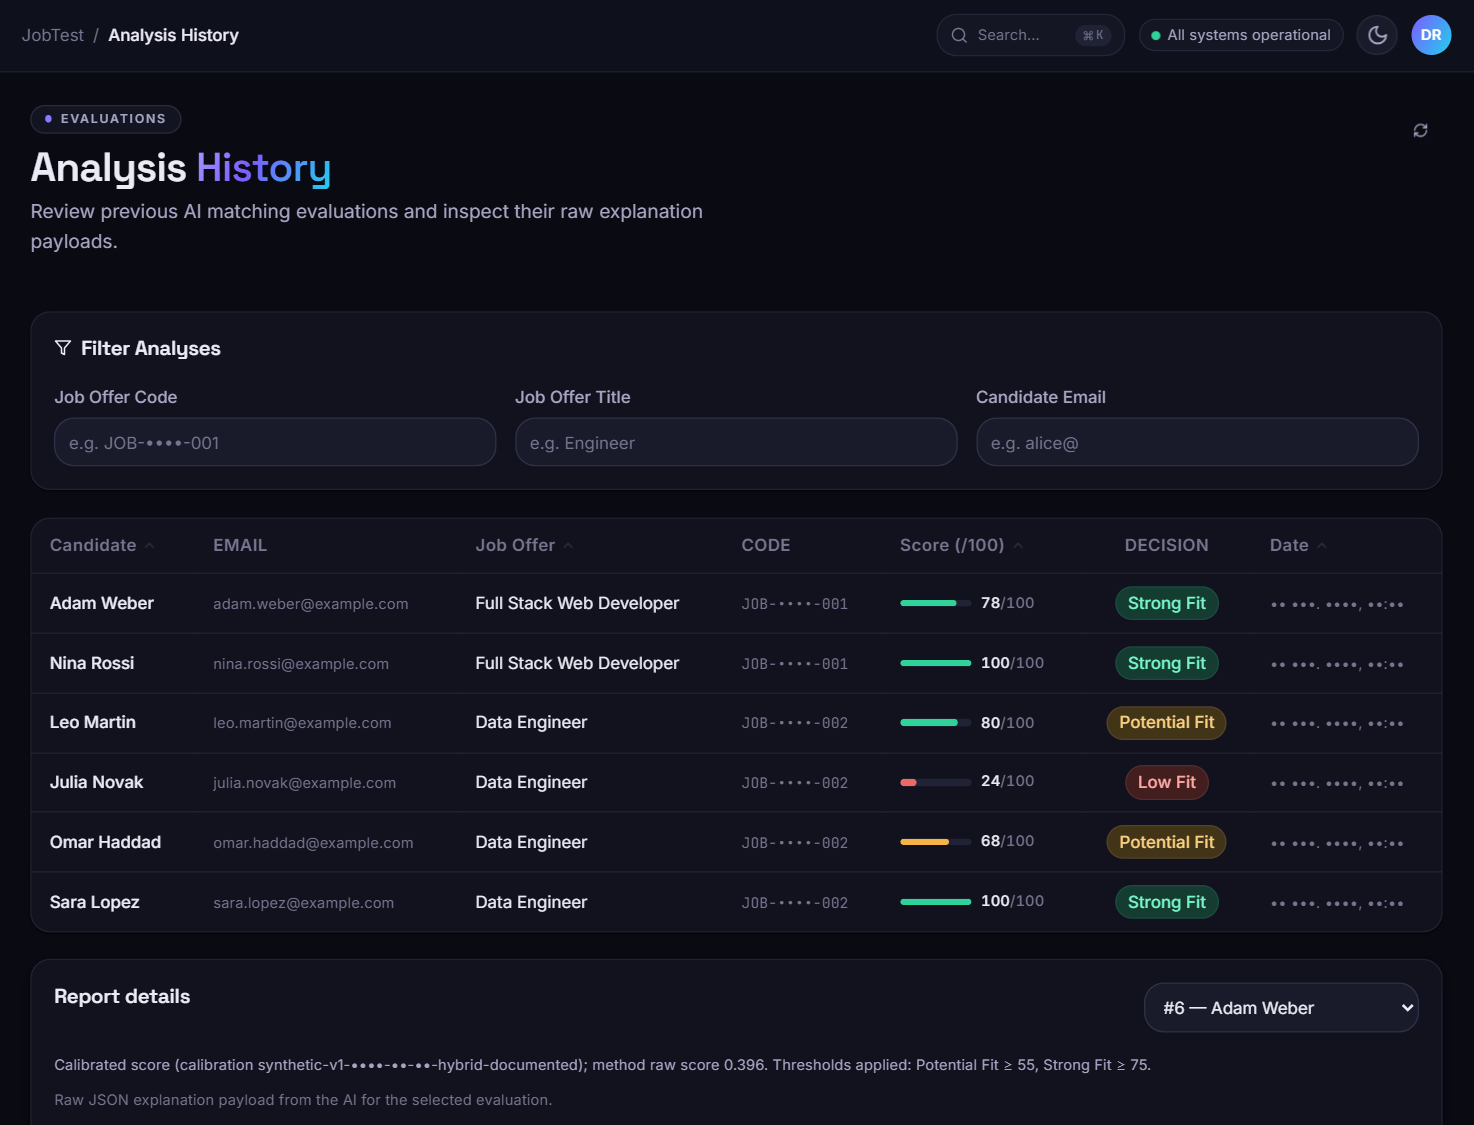
\includegraphics[width=.8\textwidth]{img/interfaces/analysis_history.png}
  \caption{Historique des évaluations}
  \label{fig:chap5-analysis-history}
\end{figure}

\subsection{Évaluation, résultat et analyse approfondie}

L'écran \emph{Candidate Analysis} constitue le point de départ du parcours principal. Il présente les compétences demandées par l'offre choisie, la politique de décision active et le bouton de lancement (figure~\ref{fig:chap5-analysis-entry}). L'exemple suivant évalue un CV fictif de développeur web face à l'offre \emph{Full Stack Web Developer}.

\begin{figure}[H]
  \centering
  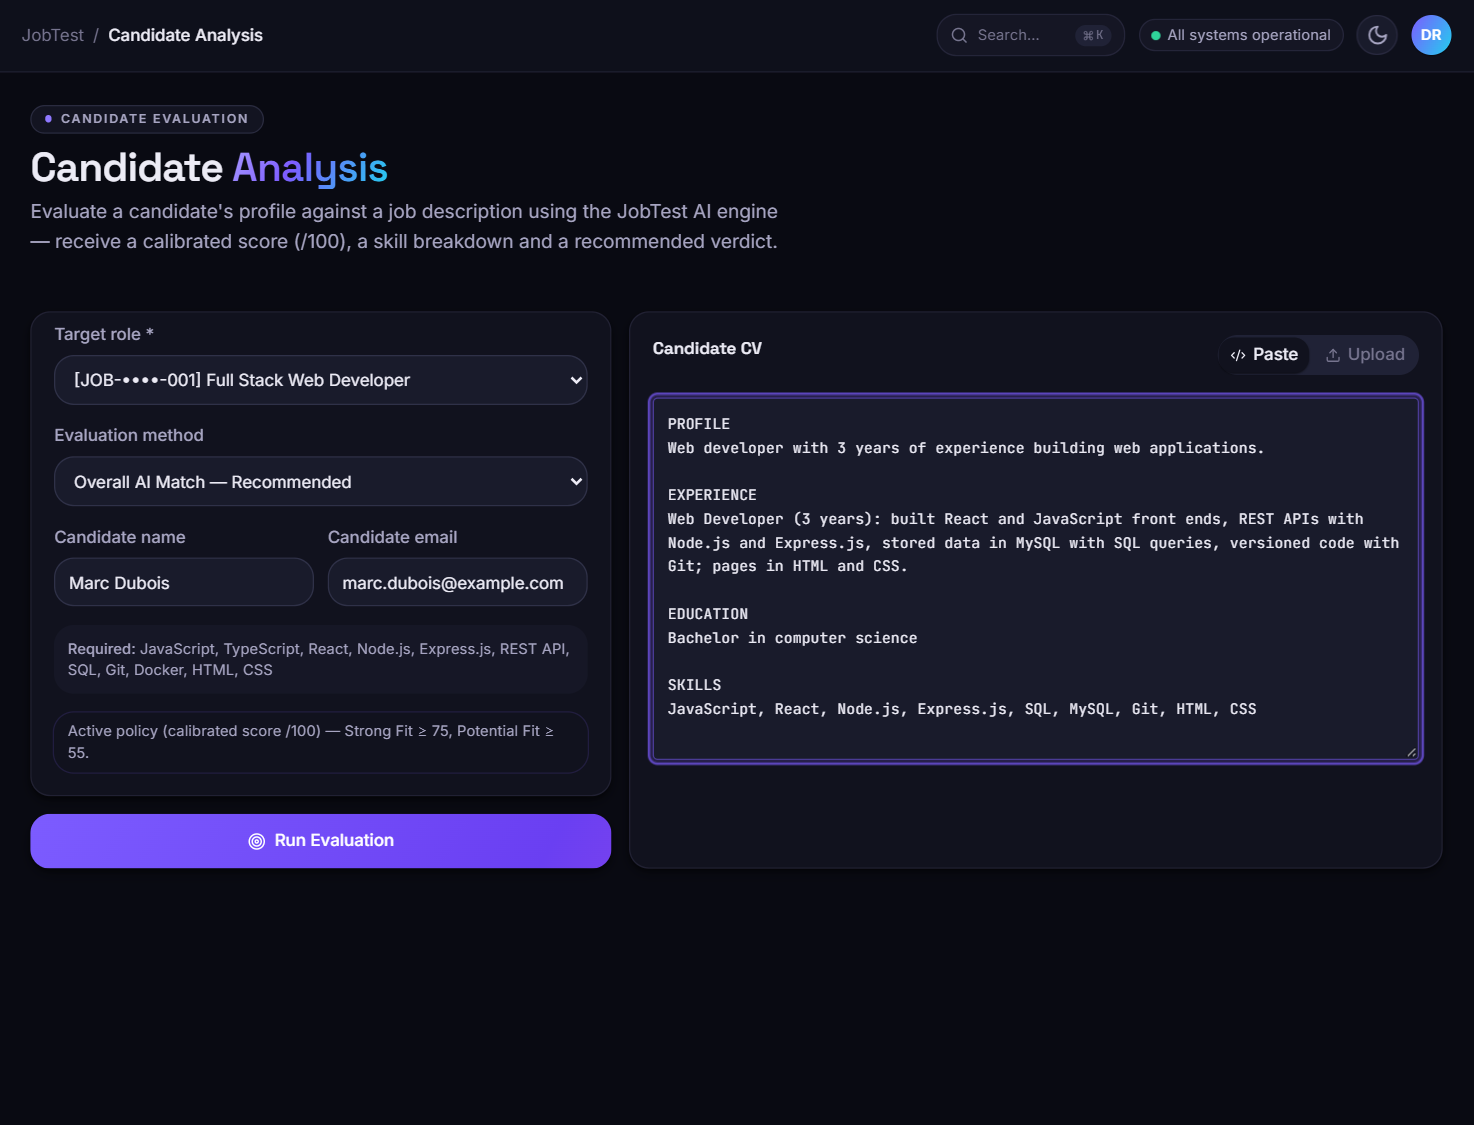
\includegraphics[width=.8\textwidth]{img/interfaces/condidate_anal_1.png}
  \caption{Saisie d'une évaluation}
  \label{fig:chap5-analysis-entry}
\end{figure}

Le résultat affiche le score calibré sur 100, le verdict recommandé, la distance au seuil le plus proche et la justification. Sous le score, une mention rappelle la version de calibration, le score brut de la méthode et les bandes appliquées. Dans cet exemple, le score brut de 0,651 dépasse la borne haute de la calibration (0,613)~: le score affiché atteint donc 100, alors que 8 des 11 compétences demandées sont reconnues. La justification signale aussi qu'une compétence exigée, TypeScript, reste à vérifier. La distance au seuil n'est pas une probabilité (figure~\ref{fig:chap5-analysis-score}).

\begin{figure}[H]
  \centering
  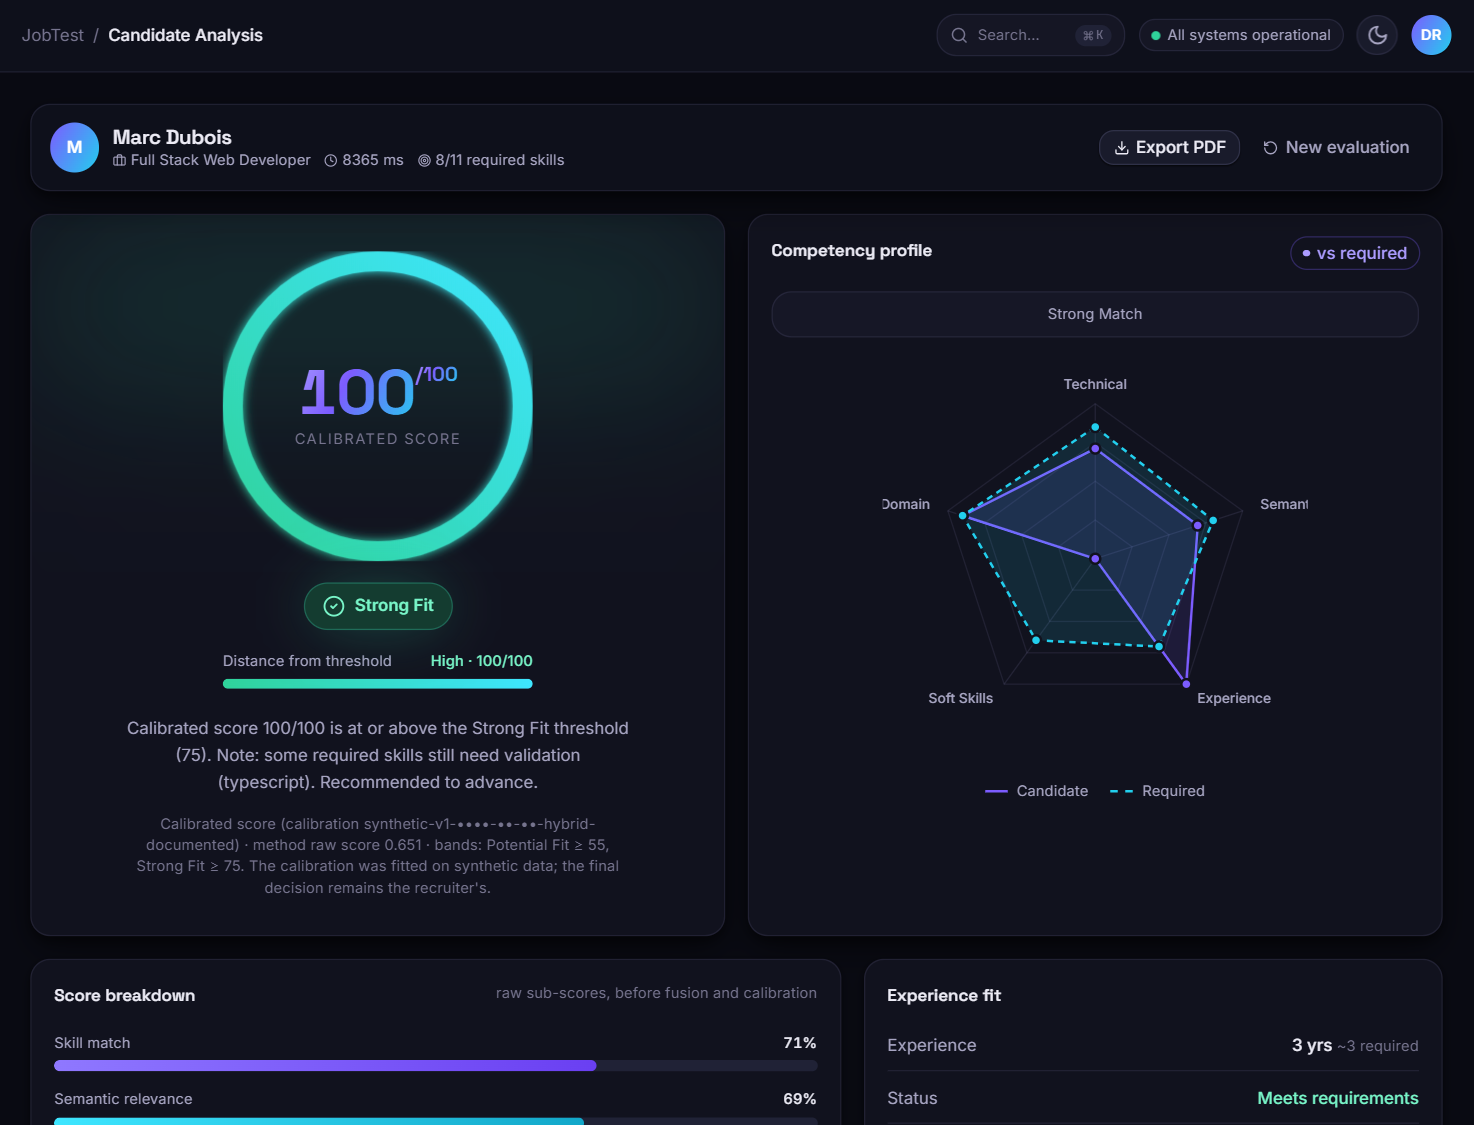
\includegraphics[width=.8\textwidth]{img/interfaces/condidate_anal_2.png}
  \caption{Score, verdict et profil de compétences}
  \label{fig:chap5-analysis-score}
\end{figure}

Les sous-scores sont présentés comme des valeurs brutes, avant fusion et calibration, à côté de l'adéquation d'expérience (figure~\ref{fig:chap5-analysis-components}). Les onglets donnent accès aux compétences, aux forces et écarts, aux actions recommandées et aux données brutes.

\begin{figure}[H]
  \centering
  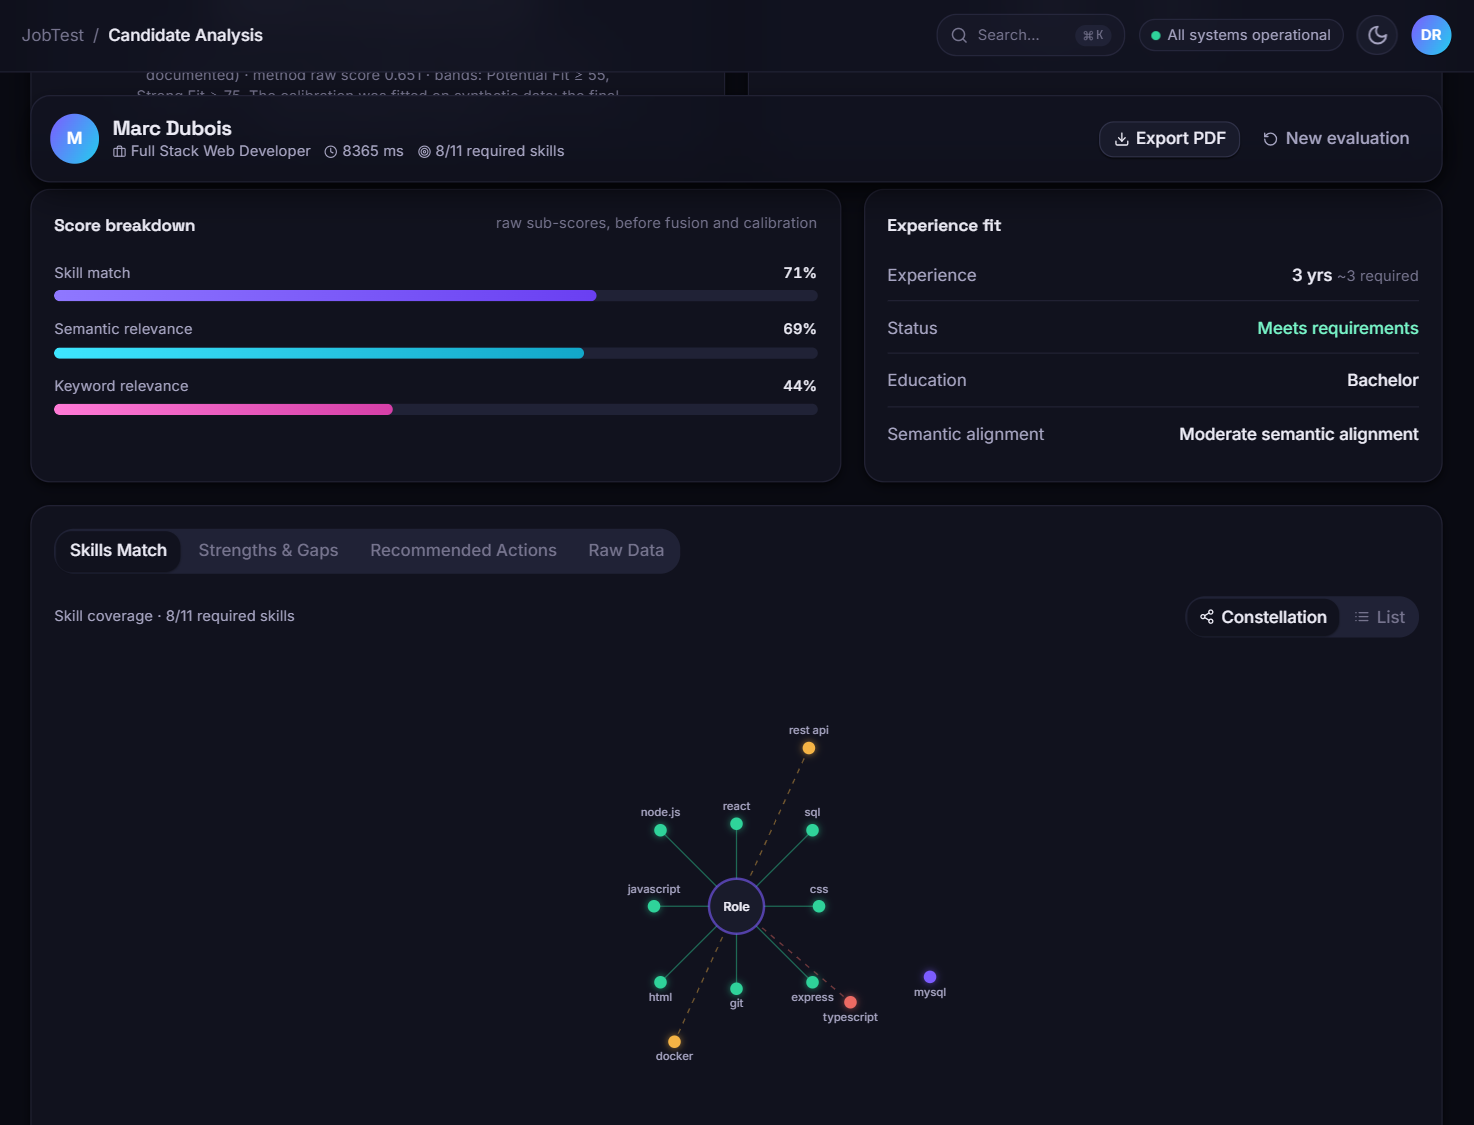
\includegraphics[width=.8\textwidth]{img/interfaces/condidate_anal_3.png}
  \caption{Sous-scores et adéquation d'expérience}
  \label{fig:chap5-analysis-components}
\end{figure}

La constellation des compétences distingue les compétences reconnues, les lacunes prioritaires, les compétences manquantes et les compétences supplémentaires du candidat (figure~\ref{fig:chap5-analysis-visualization}).

\begin{figure}[H]
  \centering
  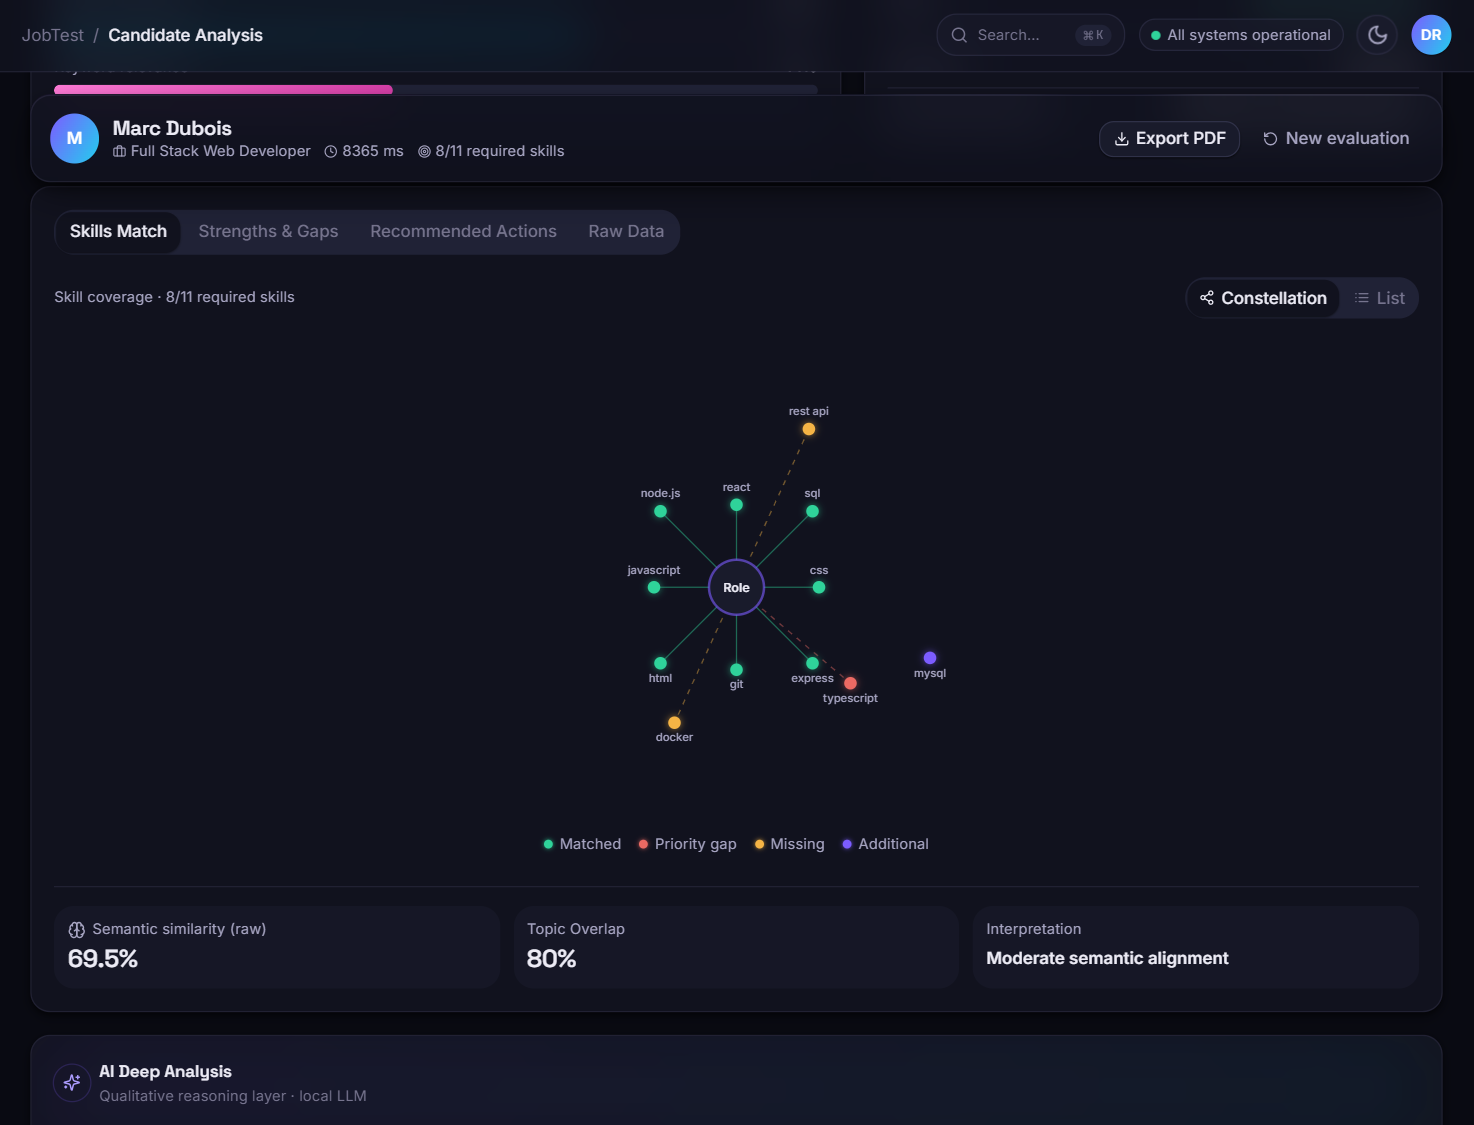
\includegraphics[width=.8\textwidth]{img/interfaces/condidate_anal_4.png}
  \caption{Compétences reconnues et manquantes}
  \label{fig:chap5-analysis-visualization}
\end{figure}

L'analyse approfondie est demandée automatiquement après l'affichage du résultat. Exécutée localement par \texttt{qwen2.5:1.5b} via Ollama, elle propose une synthèse, une trajectoire, des signaux à examiner, des recommandations et des questions d'entretien. Une mention rappelle qu'elle ne modifie ni le score ni le verdict (figure~\ref{fig:chap5-analysis-deep}). Si le runtime ne répond pas, son indisponibilité est affichée sans altérer le résultat principal.

\begin{figure}[H]
  \centering
  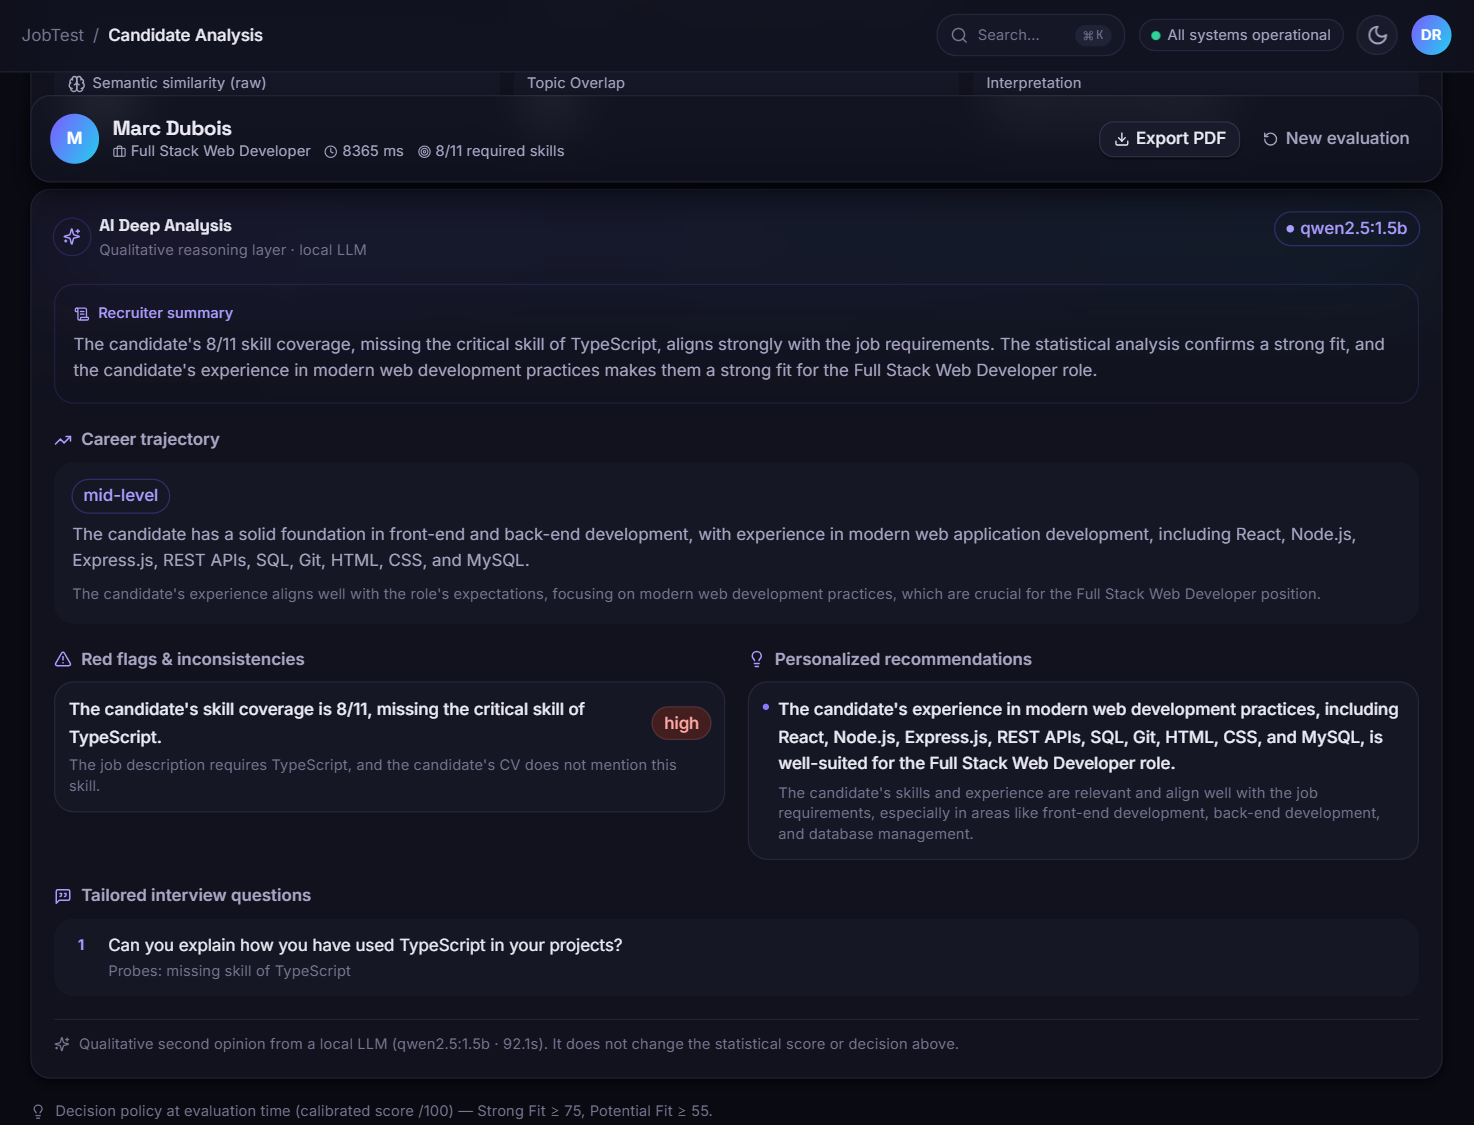
\includegraphics[width=.8\textwidth]{img/interfaces/condidate_anal_5.png}
  \caption{Analyse approfondie locale}
  \label{fig:chap5-analysis-deep}
\end{figure}

Lorsque les compétences correspondantes reposent surtout sur des déclarations ou sur du texte recopié de l'offre, un encadré \emph{Evidence check} le signale. La figure~\ref{fig:chap5-evidence} montre un CV fictif de graphiste complété par la liste des compétences de l'offre \emph{Data Engineer}~: son score calibré atteint 80,6, mais aucune des huit compétences correspondantes n'apparaît dans l'expérience décrite. Le verdict est donc limité à \emph{Potential Fit} (\texttt{CONSIDER}), avec la liste des compétences seulement déclarées.

\begin{figure}[H]
  \centering
  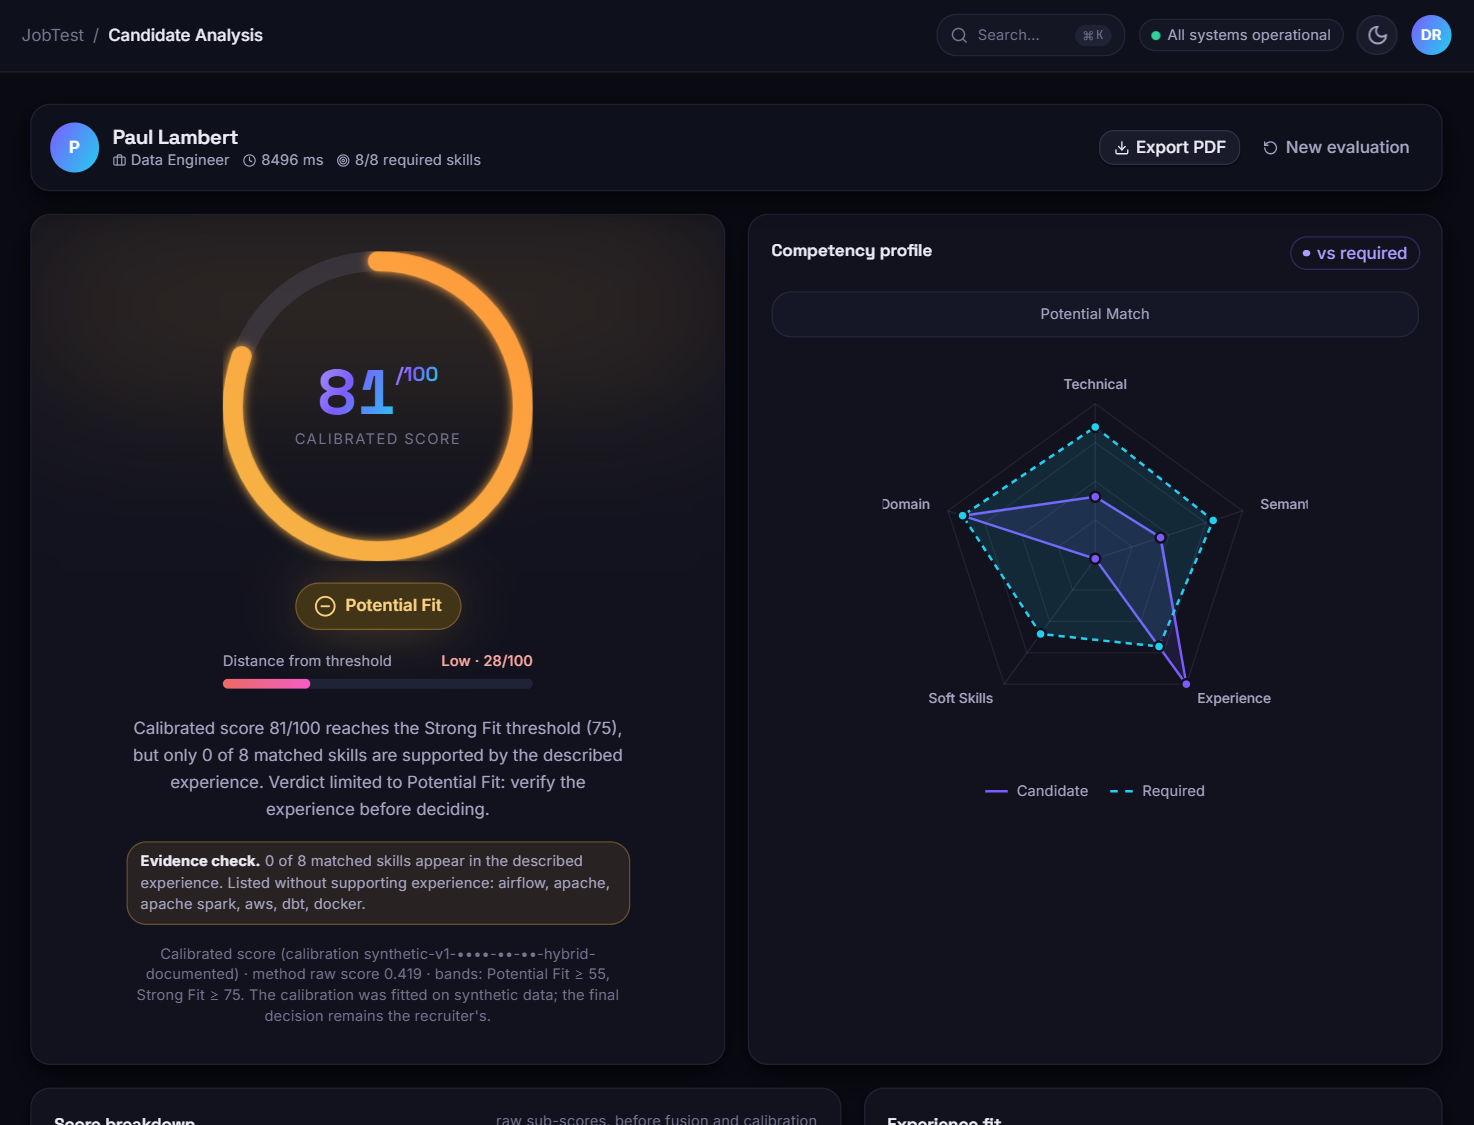
\includegraphics[width=.8\textwidth]{img/interfaces/evidence_check.png}
  \caption{Verdict limité par le contrôle des preuves}
  \label{fig:chap5-evidence}
\end{figure}

\subsection{Classement, comparaison, qualité et paramètres}

Le \emph{Talent Leaderboard} accepte plusieurs CV pour une offre et restitue un classement. Les figures~\ref{fig:chap5-leaderboard-selection} à~\ref{fig:chap5-leaderboard-result} rejouent avec la version finale l'essai décrit au chapitre~\ref{chap:tests-securite}~: dix-huit CV fictifs au format PDF face à l'offre \emph{Full Stack Web Developer}. L'export CSV du classement inclut le score calibré, le score brut, les seuils et la version de calibration.

\begin{figure}[H]
  \centering
  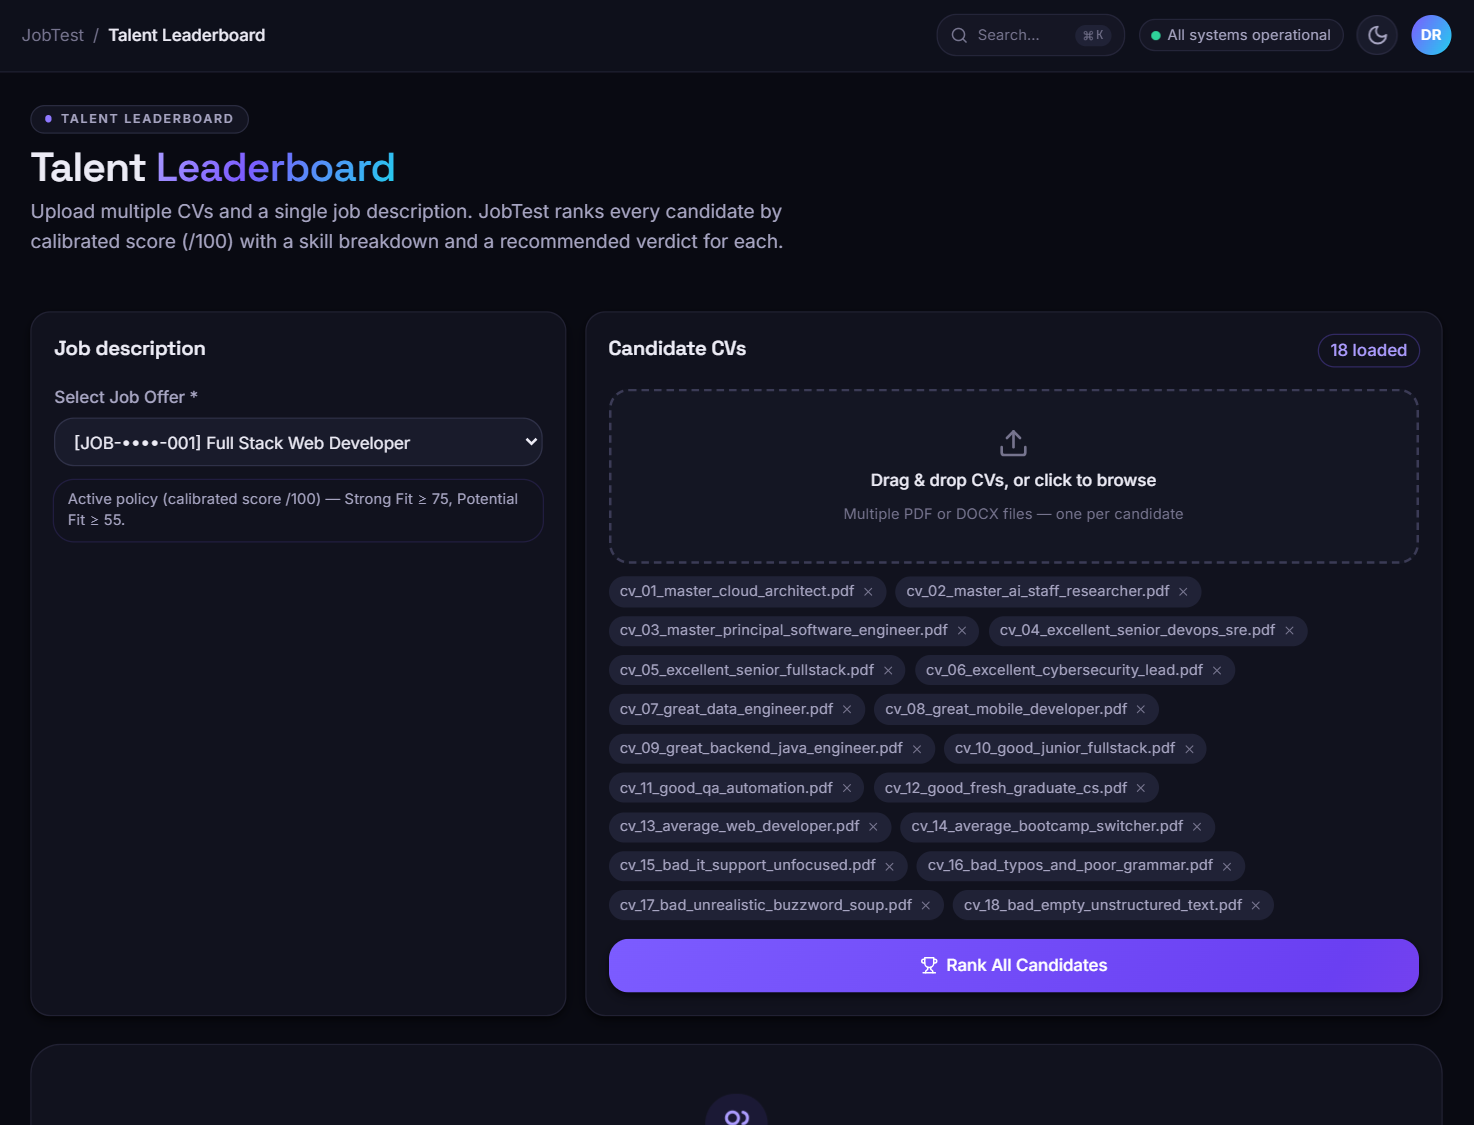
\includegraphics[width=.8\textwidth]{img/interfaces/talent_leader_1.png}
  \caption{Sélection de l'offre et des CV}
  \label{fig:chap5-leaderboard-selection}
\end{figure}

\begin{figure}[H]
  \centering
  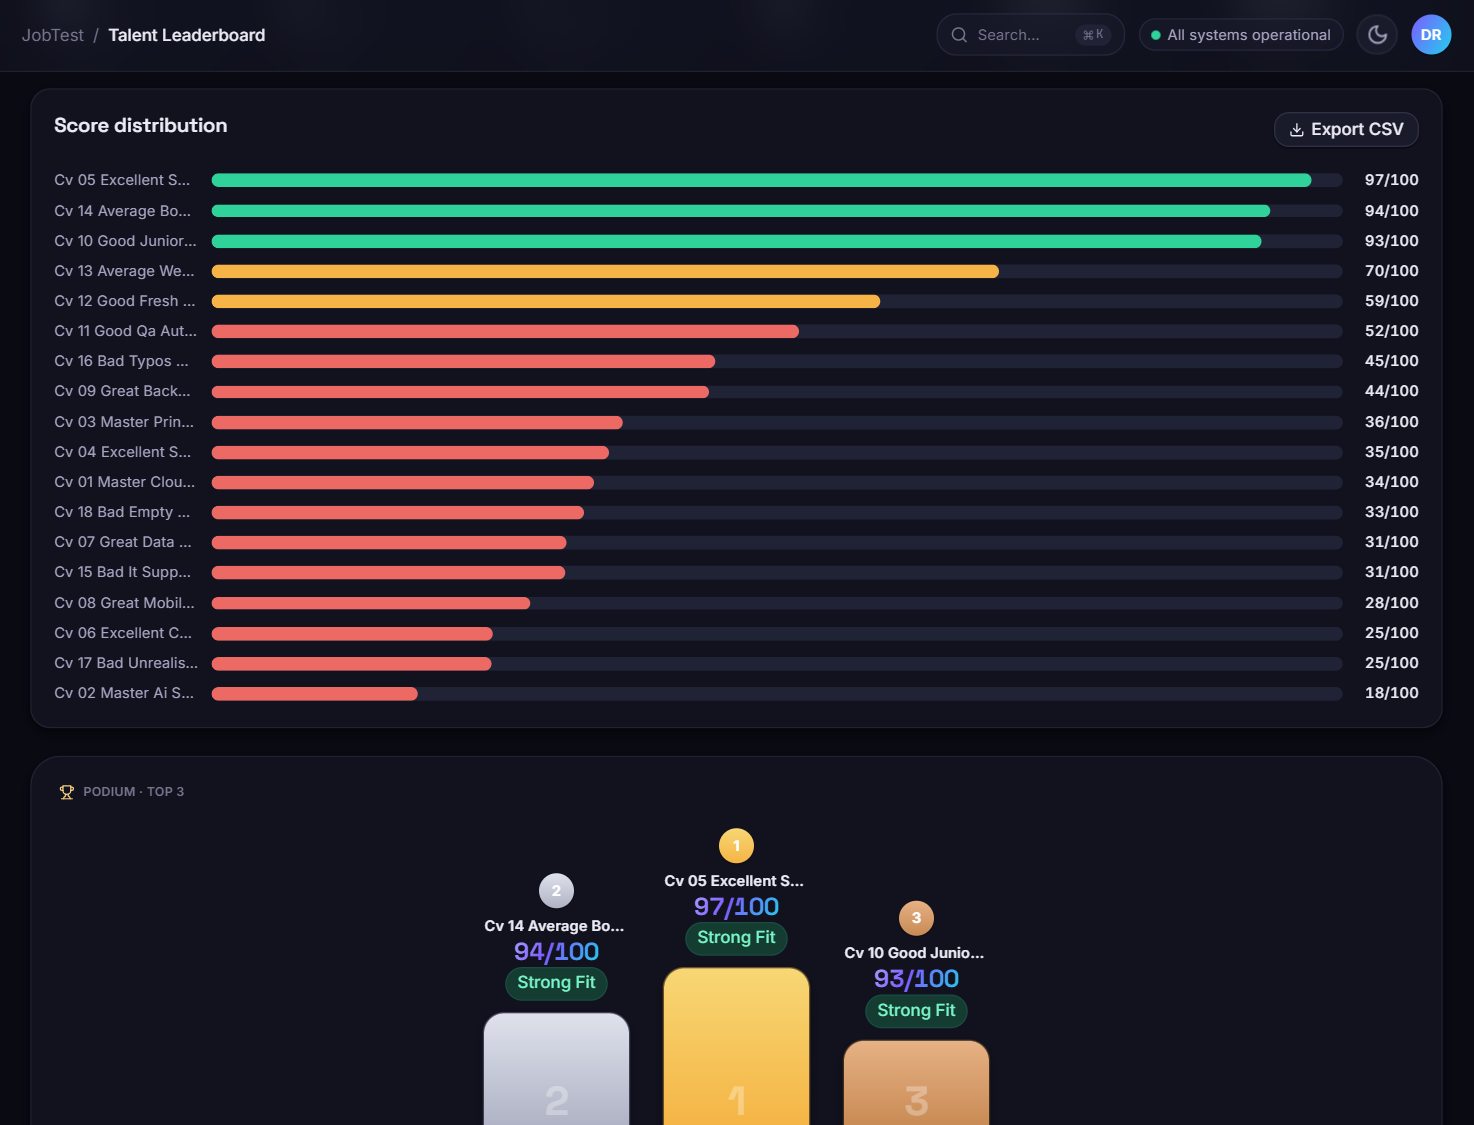
\includegraphics[width=.8\textwidth]{img/interfaces/talent_leader_2.png}
  \caption{Distribution des scores du classement}
  \label{fig:chap5-leaderboard-ranking}
\end{figure}

\begin{figure}[H]
  \centering
  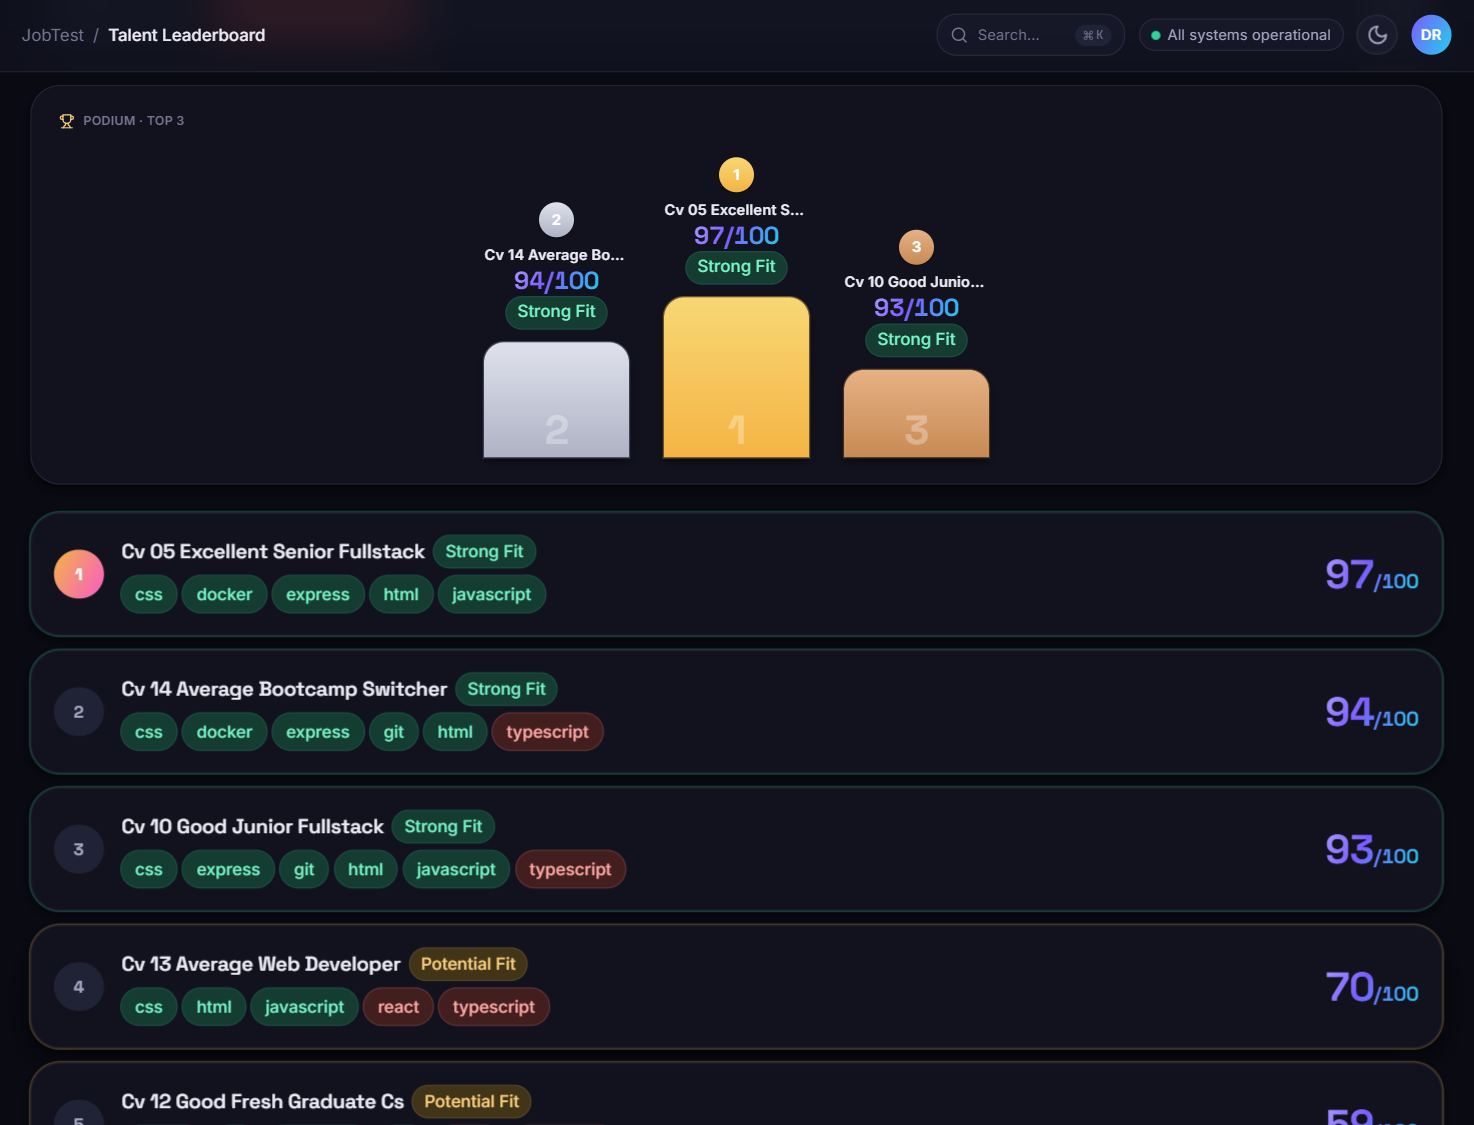
\includegraphics[width=.8\textwidth]{img/interfaces/talent_leader_3.png}
  \caption{Podium du classement}
  \label{fig:chap5-leaderboard-podium}
\end{figure}

\begin{figure}[H]
  \centering
  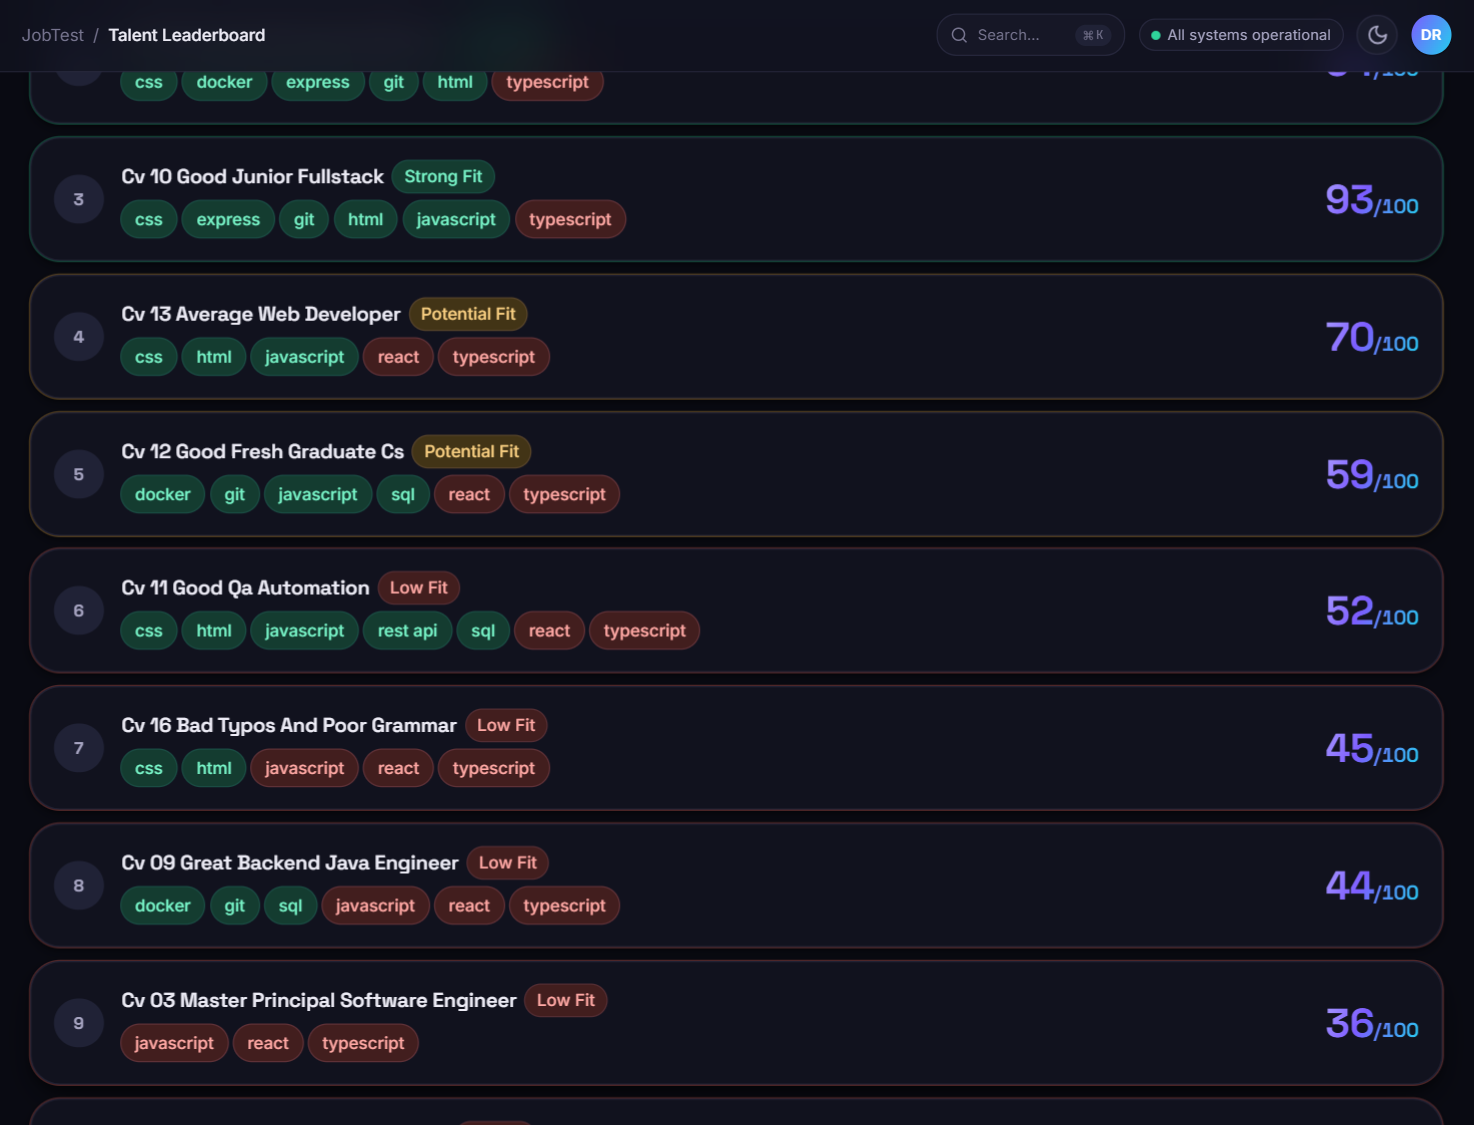
\includegraphics[width=.8\textwidth]{img/interfaces/talent_leader_4.png}
  \caption{Suite du classement}
  \label{fig:chap5-leaderboard-result}
\end{figure}

\emph{AI Insights} compare les quatre méthodes sur un même couple CV--offre sans créer de résultat persistant. Chaque score brut est ramené à l'échelle sur 100 par sa propre calibration, et les barres sont tracées sur cette échelle commune avec les bornes 55 et 75 (figure~\ref{fig:chap5-insights}).

\begin{figure}[H]
  \centering
  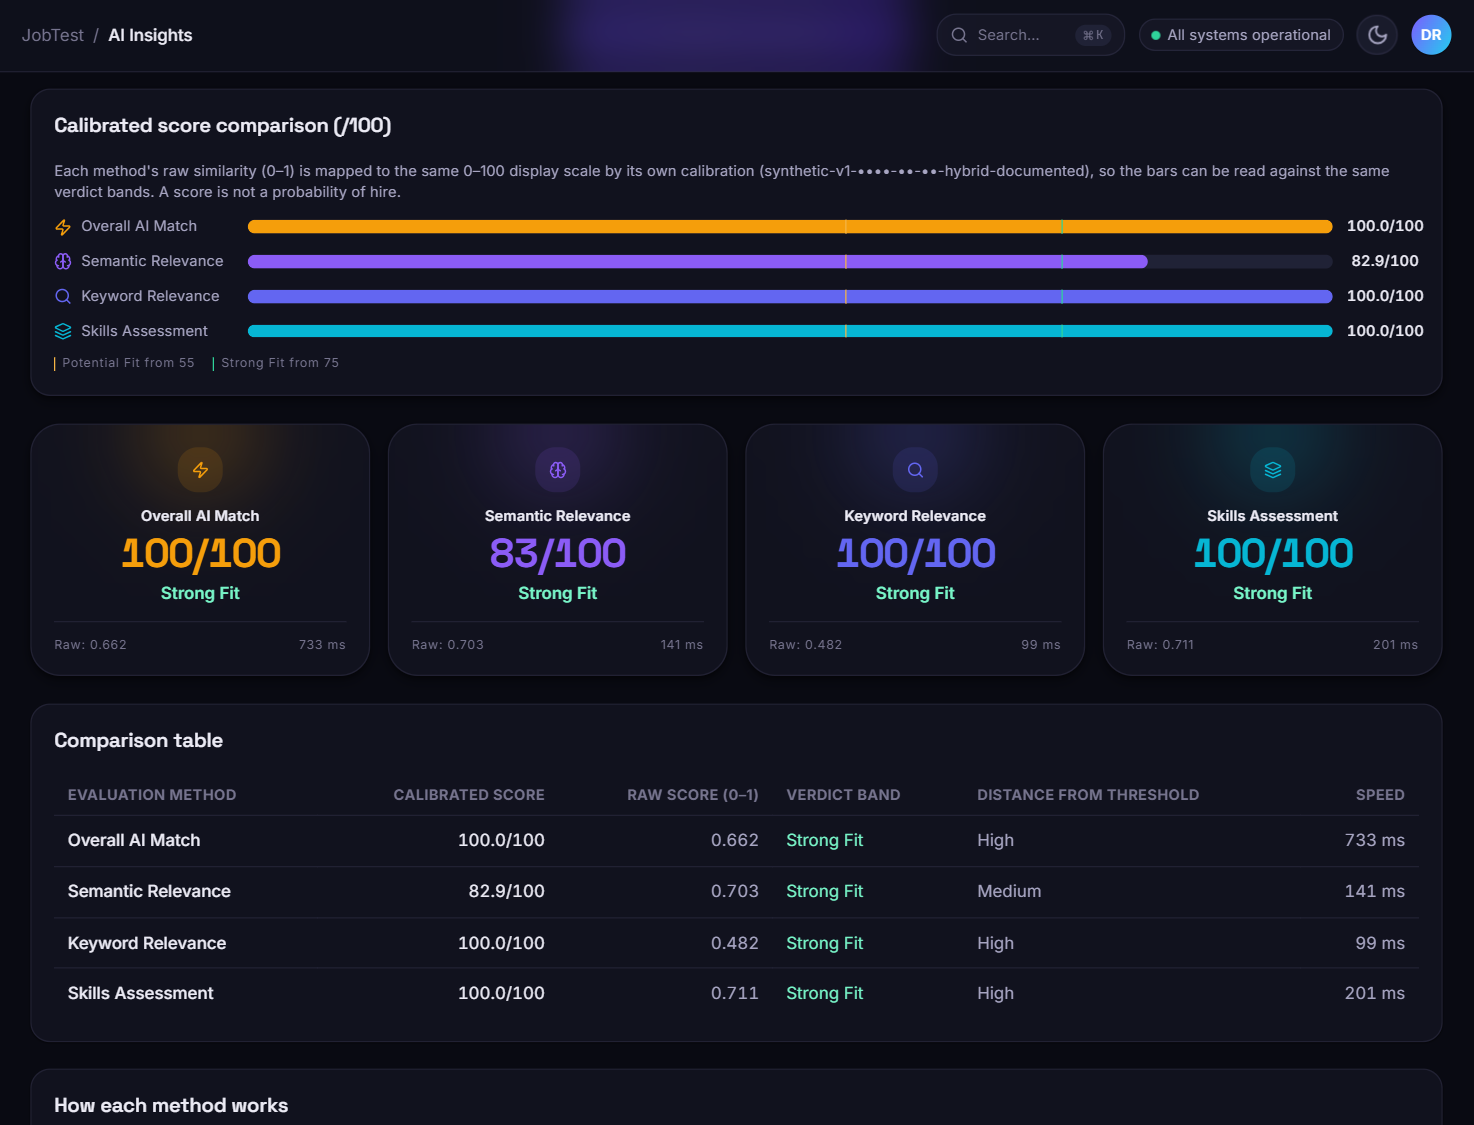
\includegraphics[width=.8\textwidth]{img/interfaces/insights.png}
  \caption{Comparaison des quatre méthodes}
  \label{fig:chap5-insights}
\end{figure}

L'écran de paramètres règle les seuils \emph{Strong Fit} et \emph{Potential Fit}, exprimés sur l'échelle calibrée, et présente l'état des composants de la plateforme (figure~\ref{fig:chap5-settings}).

\begin{figure}[H]
  \centering
  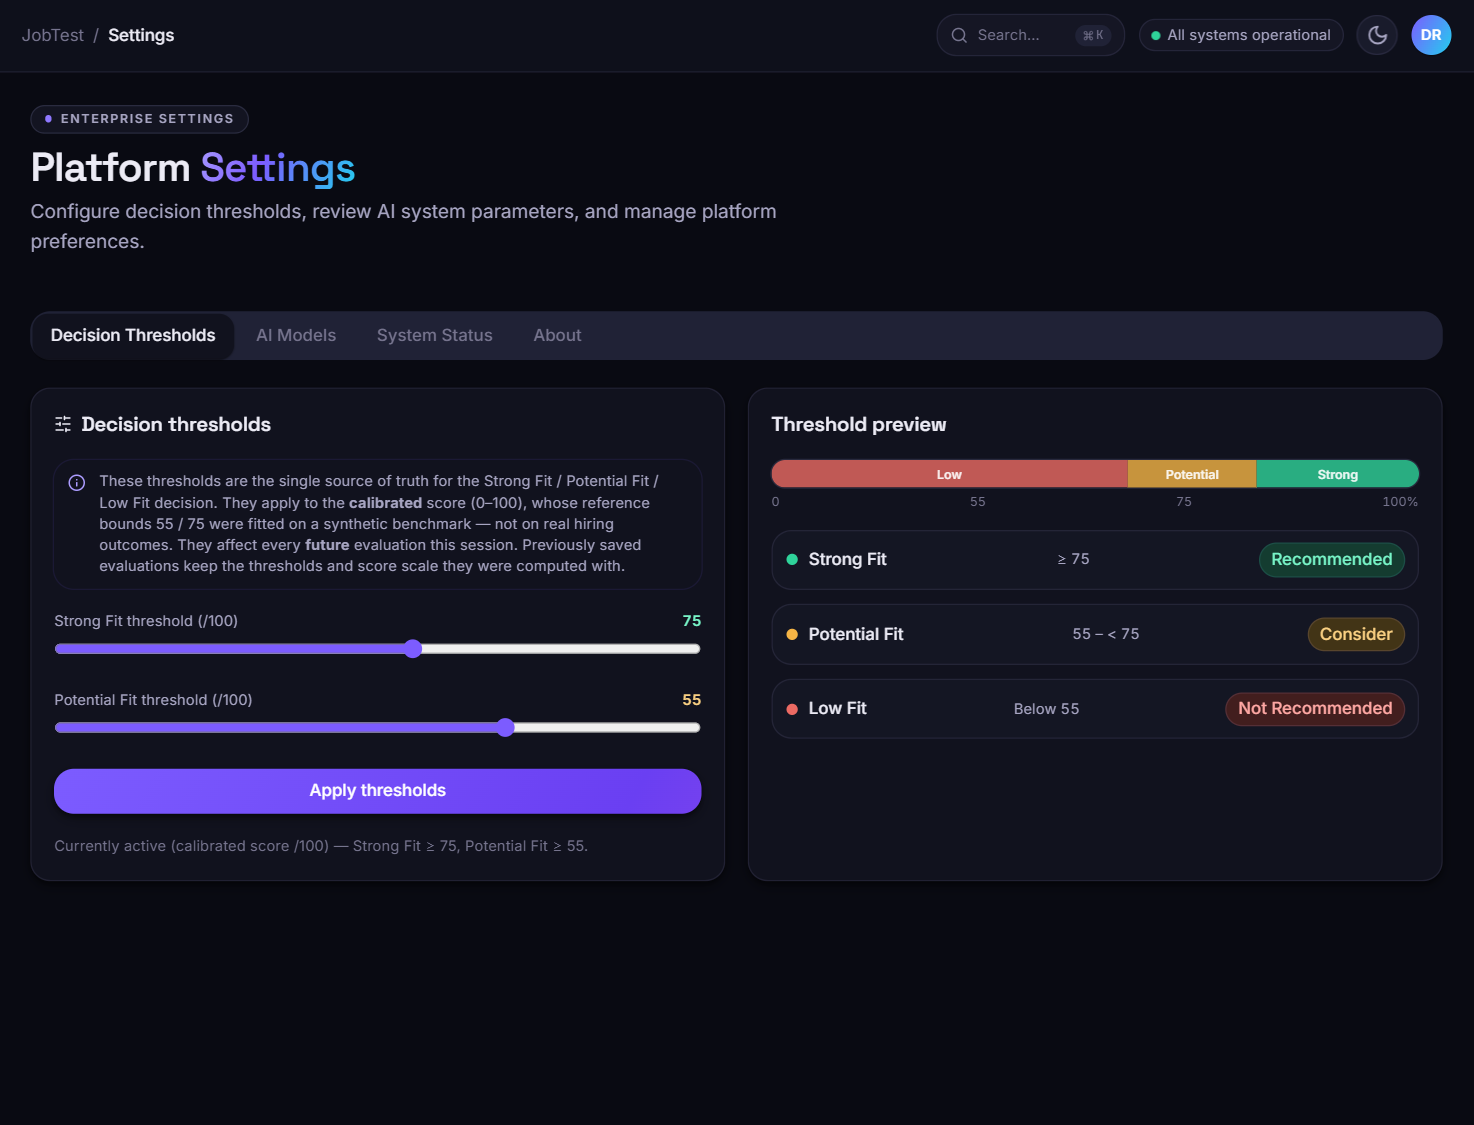
\includegraphics[width=.8\textwidth]{img/interfaces/plateform_settings.png}
  \caption{Réglage des seuils de décision}
  \label{fig:chap5-settings}
\end{figure}

L'écran \emph{AI Quality Center} présente les résultats d'évaluation hors ligne en indiquant pour chacun le fichier source, la taille de l'échantillon et sa concordance avec la calibration livrée. Il distingue trois catégories~: le banc d'essai synthétique, seul porteur de métriques~; les essais fonctionnels sur CV fictifs~; et les essais menés avec mes propres CV, pour lesquels les métriques sont affichées comme non mesurées (figure~\ref{fig:chap5-quality-1}).

\begin{figure}[H]
  \centering
  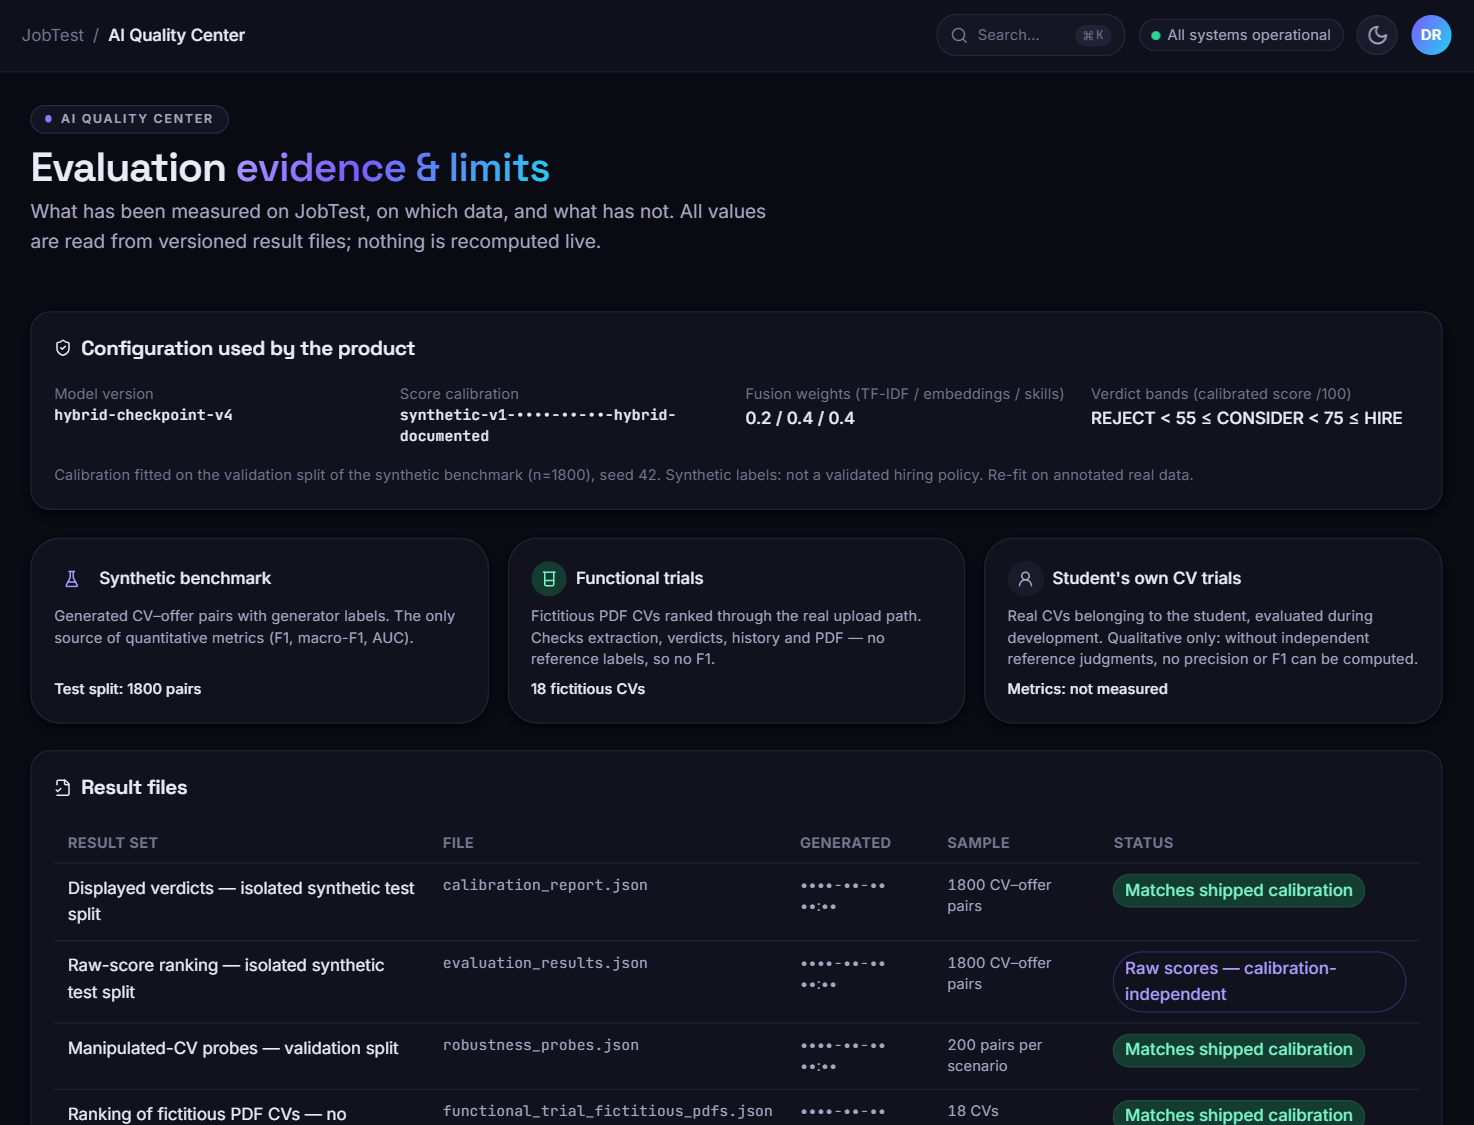
\includegraphics[width=.8\textwidth]{img/interfaces/quality_1.png}
  \caption{\emph{AI Quality Center}~: configuration}
  \label{fig:chap5-quality-1}
\end{figure}

La qualité des verdicts affichés (macro-F1 à trois classes) et la qualité du classement du score brut (F1 binaire à un seuil expérimental) y sont présentées dans deux tableaux distincts, avec leurs définitions et la matrice de confusion de la version livrée (figure~\ref{fig:chap5-quality-2}). Une dernière partie reprend les essais de robustesse face aux CV manipulés (figure~\ref{fig:chap5-quality-3}). Toutes ces valeurs sont lues dans les fichiers versionnés du dossier \texttt{evaluation/results}~; une métrique absente est affichée comme non mesurée, jamais comme nulle.

\begin{figure}[H]
  \centering
  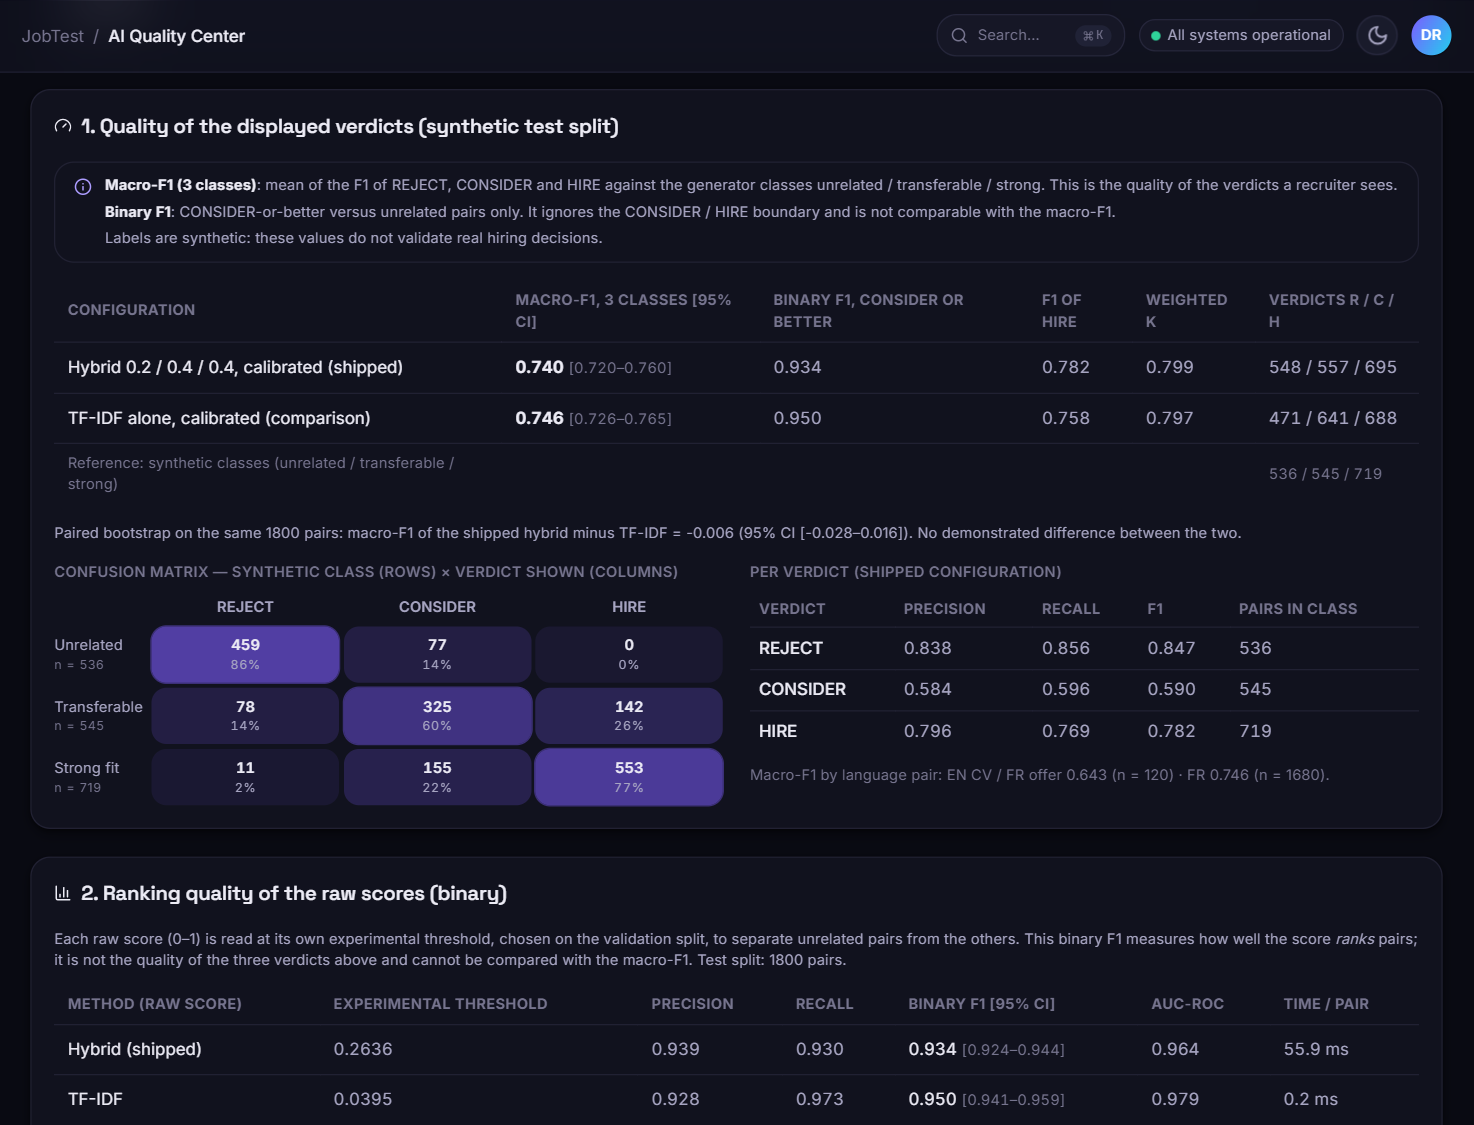
\includegraphics[width=.8\textwidth]{img/interfaces/quality_2.png}
  \caption{\emph{AI Quality Center}~: qualité des verdicts}
  \label{fig:chap5-quality-2}
\end{figure}

\begin{figure}[H]
  \centering
  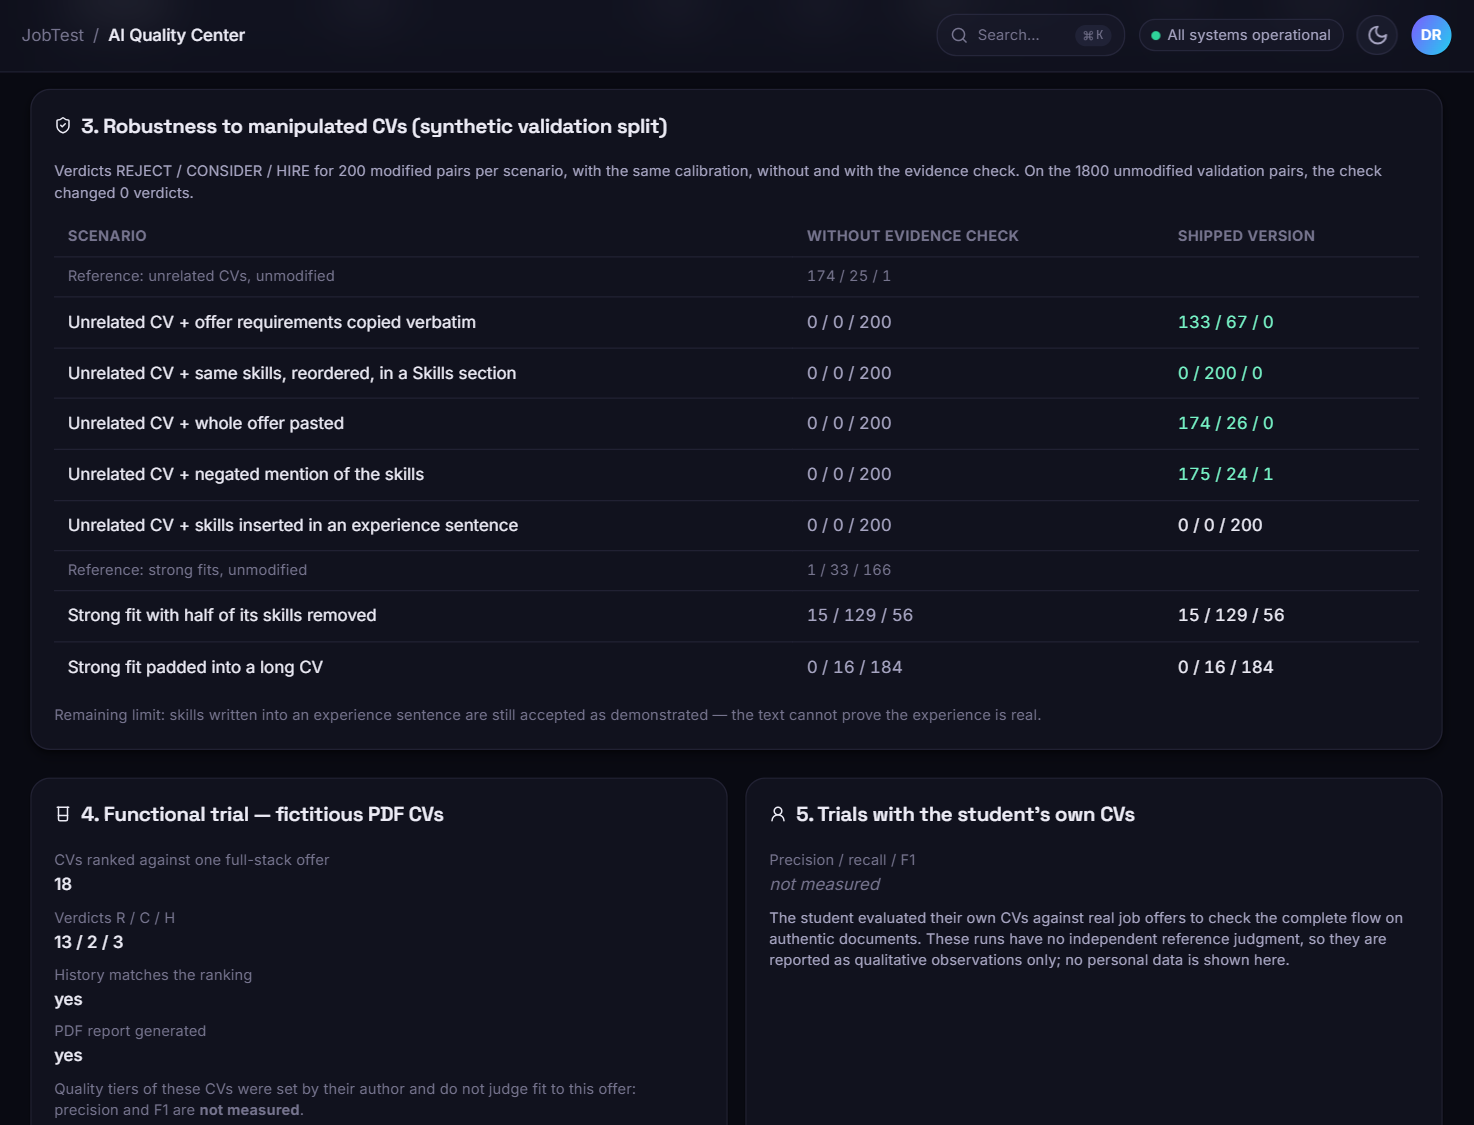
\includegraphics[width=.8\textwidth]{img/interfaces/quality_3.png}
  \caption{\emph{AI Quality Center}~: robustesse}
  \label{fig:chap5-quality-3}
\end{figure}

Enfin, le bouton \emph{Export PDF} de l'écran de résultat déclenche la génération ReportLab et le téléchargement du rapport. Le document reprend les éléments de décision déjà visibles, au lieu de fournir une décision autonome supplémentaire.

\section{Parcours fonctionnel de démonstration}

Un scénario de démonstration se déroule de façon continue : le recruteur se connecte, crée ou sélectionne une offre ouverte, fournit le texte ou le fichier d'un CV, puis lance l'évaluation. Il lit ensuite le score et les raisons associées, consulte si besoin l'analyse approfondie, puis exporte le rapport PDF. L'historique permet enfin de retrouver une évaluation persistée. Ce parcours maintient une séparation claire entre les données métier (offre, candidat et CV), le calcul de correspondance et l'aide à l'interprétation.

\section{Difficultés de réalisation et solutions apportées}

Les difficultés retenues ci-dessous sont celles qui apparaissent dans le code ou dans l'historique technique du projet. Elles concernent la réalisation de la plateforme, non les incidents de déploiement qui seront détaillés au chapitre suivant.

Le tableau~\ref{tab:chap5-difficulties} les présente avec la réponse apportée à chacune.

\begin{table}[H]
\centering
\small
\caption{Difficultés et solutions}
\label{tab:chap5-difficulties}
\begin{tabularx}{\textwidth}{|p{0.27\textwidth}|p{0.28\textwidth}|X|}
\hline
\textbf{Difficulté} & \textbf{Conséquence} & \textbf{Solution retenue}\\
\hline
Prototype Streamlit et interface finale distincts & Risque que le moteur ne soit pas accessible par l'interface Web actuelle. & Création du routeur \texttt{/api/v1/ui}, réutilisant les services métier existants depuis Next.js.\\
\hline
CV PDF et DOCX hétérogènes & Extraction incomplète possible selon le document. & Parsers dédiés avec replis PDF et DOCX avant le prétraitement commun.\\
\hline
Modèles d'embeddings indisponibles ou contraints & Le composant sémantique ne doit pas empêcher le service de répondre. & Chargement différé et stratégie de repli locale documentée dans le moteur.\\
\hline
Layer 2 potentiellement lente ou indisponible & Une réponse LLM ne doit pas bloquer le verdict calculé. & Appel séparé, enveloppe d'état contrôlée et conservation du niveau 1 comme source du score.\\
\hline
Évolution SQLite vers PostgreSQL & Les entités et relations doivent rester cohérentes entre environnements. & Modèles SQLAlchemy communs et configuration par URL de base de données.\\
\hline
Export exploitable hors application & Le recruteur doit partager une synthèse lisible. & Génération serveur ReportLab à partir du résultat déjà obtenu.\\
\hline
\end{tabularx}
\end{table}

\section*{Conclusion}

JobTest est réalisé comme une plateforme Web modulaire dans laquelle Next.js porte le parcours du recruteur et FastAPI centralise les règles métier, les calculs et la persistance. Les écrans transforment un résultat de matching en éléments interprétables : score, compétences, explications, recommandations, analyse qualitative conditionnelle et rapport PDF. Le système soutient ainsi l'évaluation du recruteur sans se substituer à sa décision. Le chapitre suivant présentera les tests, les mesures de sécurité, la conteneurisation et le déploiement Azure.

        \clearpage
        \chapter{Tests, sécurité, DevOps et déploiement Azure}
\label{chap:tests-securite}

\section*{Introduction}

Après la réalisation de la plateforme, sa valeur dépend autant de la fiabilité de la chaîne complète que de la cohérence du moteur de rapprochement. Ce chapitre présente les contrôles effectivement disponibles dans JobTest, les vérifications effectuées lors du déploiement et les protections visibles dans le code et la configuration. Il distingue les tests automatisés, les vérifications manuelles et les observations ponctuelles faites sur la machine de démonstration. L'objectif n'est pas de certifier une disponibilité de production, mais de documenter de manière traçable le périmètre validé, les choix d'exploitation et les limites restantes.

\section{Stratégie de validation}

La validation combine une suite \texttt{pytest}, des contrôles d'API et une vérification de bout en bout sur l'environnement conteneurisé. Les essais de benchmark du chapitre 4 restent séparés : ils étudient un corpus synthétique et ne constituent pas une suite de tests fonctionnels. Le tableau \ref{tab:chap6-validation-strategy} synthétise le statut des éléments examinés.

\begin{table}[H]
\centering
\small
\caption{Niveaux de validation retenus pour JobTest}
\label{tab:chap6-validation-strategy}
\begin{tabularx}{\textwidth}{|p{.12\textwidth}|p{.18\textwidth}|X|p{.14\textwidth}|}
\hline
\textbf{Niveau} & \textbf{Objectif} & \textbf{Outil ou méthode} & \textbf{Statut}\\
\hline
Unitaires & Vérifier extraction, fusion, décision, PDF et règles de cohérence. & \texttt{pytest} ; modèles de langue et Ollama simulés lorsque nécessaire. & Partiel : 106 réussites sur 113 items.\\
\hline
API et intégration & Vérifier routes, statuts HTTP, JWT, persistance et contrats. & Tests FastAPI et contrôles d'API documentés. & Partiel : 6 tests hérités à adapter.\\
\hline
Fonctionnel & Vérifier le parcours recruteur depuis l'inscription jusqu'au rapport. & Scénario manuel enregistré sur la VM Azure. & Réalisé sur un jeu synthétique.\\
\hline
Chaîne IA & Vérifier sous-scores, verdict, explication et statut de la couche 2. & Tests du moteur, réponses de l'API et contrôle du résultat persistant. & Réalisé ; benchmark distinct au chapitre 4.\\
\hline
Déploiement & Vérifier les conteneurs, le proxy, les health checks et les ports. & \texttt{docker compose}, \texttt{nginx -t}, requêtes HTTP et journaux. & Réalisé ponctuellement.\\
\hline
\end{tabularx}
\end{table}

Le dernier lancement documenté de \texttt{pytest -q} a produit 106 tests réussis, 6 échecs et 1 test ignoré (113 items, environ 45 secondes). Les six échecs sont concentrés dans \texttt{test\_api\_extended.py} : des fixtures de routes historiques ne satisfont plus le contrôle d'appartenance introduit pour les offres et résultats. Ils retournent donc \texttt{404} au lieu du résultat attendu par ces tests anciens. Ce constat ne permet pas de déclarer la suite entièrement verte ; sa mise à jour constitue une action de maintenance.

\section{Environnement et données de test}

Le développement a été conduit localement sous Windows avec Python, Node.js et SQLite, puis vérifié dans une topologie Docker Compose utilisant PostgreSQL. La validation intégrée a ensuite été observée sur une machine virtuelle Azure. Les parcours fonctionnels ont utilisé un compte recruteur de démonstration, une offre et un CV synthétiques. Aucun résultat présenté dans ce chapitre ne requiert l'affichage d'un mot de passe, d'un jeton, d'une clé SSH, d'une chaîne de connexion ou du contenu du fichier \texttt{.env}. Les éléments visibles dans les traces de déploiement sont des données de vérification et non un jeu de CV réels.

\section{Tests fonctionnels}

La matrice suivante reprend seulement les scénarios dont l'exécution ou le résultat est attesté par les tests du dépôt ou le rapport de déploiement. Les cas non exécutés ne sont pas convertis artificiellement en succès.

Le tableau~\ref{tab:chap6-functional-matrix} en dresse la liste.

{\scriptsize
\begin{longtable}{|p{.06\textwidth}|p{.18\textwidth}|p{.19\textwidth}|p{.23\textwidth}|p{.18\textwidth}|p{.08\textwidth}|}
\caption{Matrice des contrôles fonctionnels attestés}\label{tab:chap6-functional-matrix}\\
\hline
\textbf{ID} & \textbf{Fonction} & \textbf{Précondition} & \textbf{Résultat attendu} & \textbf{Résultat obtenu} & \textbf{Statut}\\
\hline
\endfirsthead
\hline
\textbf{ID} & \textbf{Fonction} & \textbf{Précondition} & \textbf{Résultat attendu} & \textbf{Résultat obtenu} & \textbf{Statut}\\
\hline
\endhead
F01 & Inscription et connexion & Compte de vérification. & Création puis obtention d'un jeton sans l'exposer. & Compte créé et JWT utilisé pendant la vérification Azure. & OK\\
\hline
F02 & Refus d'identifiants invalides & Identifiants incorrects. & Réponse d'authentification refusée. & Couvert par les tests \texttt{test\_auth}. & OK\\
\hline
F03 & Consultation du profil & Jeton Bearer valide. & Retour du recruteur connecté. & Route protégée couverte par les tests d'authentification. & OK\\
\hline
F04 & Création d'offre & Recruteur authentifié. & Offre enregistrée et rattachée au recruteur. & Offre de contrôle créée (identifiant 1 dans l'environnement observé). & OK\\
\hline
F05 & Évaluation d'un CV & Offre et CV de démonstration. & Sous-scores, explication et recommandation générés. & Résultat \texttt{MatchResult} 1 créé, verdict \texttt{CONSIDER}. & OK\\
\hline
F06 & Persistance & Évaluation réussie. & Résultat récupérable avec relations cohérentes. & Un résultat et une analyse LLM valide comptabilisés dans PostgreSQL. & OK\\
\hline
F07 & Analyse approfondie & Résultat persistant, Ollama disponible. & Enveloppe d'analyse sans modification du score. & \texttt{status=ok} observé et analyse enregistrée. & OK\\
\hline
F08 & Rapport PDF & Résultat calculé. & Flux PDF ouvrable avec informations d'évaluation. & PDF 1.4, deux pages et 112\,039 octets dans ce cas. & OK\\
\hline
F09 & Routes API historiques & Fixtures anciennes de test. & Réponse des routes historiques. & Six attentes sont incompatibles avec le contrôle de propriété. & À adapter\\
\hline
\end{longtable}
}

\section{Validation du moteur intelligent}

Le contrôle fonctionnel du moteur concerne ici sa mise en œuvre, non la qualité prédictive discutée au chapitre 4. Une évaluation retournée par l'API contient les trois sous-scores utilisés dans la fusion, les paramètres de pondération, l'explication structurée et la recommandation algorithmique. Les tests couvrent la fusion hybride, les frontières de décision, la cohérence entre moteur et module d'explication ainsi que les états \texttt{disabled}, \texttt{unavailable}, \texttt{error}, \texttt{ok} et \texttt{inconsistent} de la couche 2.

La couche générative reçoit le résultat déterministe mais ne calcule ni le score officiel ni le verdict \texttt{HIRE}, \texttt{CONSIDER} ou \texttt{REJECT}. Les tests de raisonnement emploient un Ollama simulé ; la disponibilité réelle de la couche 2 a, elle, été vérifiée une fois sur Azure. Les cas de CV vide, d'offre inexistante et de ressources appartenant à un autre recruteur sont contrôlés par les routes concernées. Les résultats de cas de seuil exact 55 ou 75 ne sont pas présentés séparément ici, faute de trace de démonstration dédiée.

\section{Tests de l'API et de la persistance}

Les schémas Pydantic valident les corps de requête et FastAPI retourne notamment des erreurs \texttt{401}, \texttt{404}, \texttt{422} ou \texttt{429} selon le contrat concerné. Chaque route de données passe par l'authentification Bearer. La fonction \texttt{\_assert\_owned} vérifie que l'offre et le candidat visés appartiennent au recruteur connecté ; une ressource d'un autre périmètre est traitée comme absente. Les requêtes courantes sont exprimées par SQLAlchemy plutôt que par concaténation de SQL ; cette pratique réduit l'exposition à des chaînes SQL construites manuellement, sans constituer à elle seule une garantie universelle.

La vérification Azure a confirmé l'écriture d'un \texttt{MatchResult} et d'une analyse LLM valide, puis leur comptage dans PostgreSQL. Les relations candidat, offre et résultat ont donc été parcourues dans un scénario réel de démonstration. Swagger était accessible derrière Nginx à \texttt{/api/v1/docs}; aucune capture n'est ajoutée afin d'éviter de répéter les écrans du chapitre 5.

\section{Validation du rapport PDF}

La génération est testée dans le dépôt par des contrôles de structure binaire et a également été validée dans le parcours déployé. Pour un résultat précis, la réponse HTTP a été reçue sous forme de PDF 1.4, le fichier s'est ouvert sur deux pages et sa taille était de 112\,039 octets. Ces valeurs caractérisent un exemple de démonstration : le nombre de pages et le poids peuvent évoluer avec les données du candidat et de l'offre. L'export utilise les informations déjà calculées ; il ne lance pas un nouveau rapprochement.

\section{Tests de santé et stabilité des services}

Les cinq conteneurs ont été observés à l'état \emph{healthy}, avec une politique \texttt{unless-stopped} et sans redémarrage inattendu lors du contrôle. La configuration Nginx a passé \texttt{nginx -t}; l'accueil et Swagger ont retourné HTTP 200 via le proxy. L'endpoint FastAPI de santé et son contrôle détaillé ont retourné \texttt{ok}; la couche 1 était disponible, Ollama répondait et le modèle \texttt{qwen2.5:1.5b} était installé. Les journaux examinés ne montraient ni OOM, ni erreur fatale, ni boucle de redémarrage. Il s'agit d'une observation à un instant donné et non d'un engagement de disponibilité permanente.

\section{Résultats de validation de bout en bout}

Le scénario intégré attesté suit les étapes suivantes : utilisation d'un compte recruteur, authentification, création d'une offre, évaluation d'un CV synthétique, enregistrement du résultat, lecture de l'explication, analyse approfondie puis génération du PDF servi par Nginx. Cette chaîne a produit les trois composantes de score, une recommandation \texttt{CONSIDER}, un \texttt{MatchResult} persistant, une analyse LLM \texttt{ok} et le rapport PDF décrit précédemment.

La mesure de l'analyse approfondie est de 54\,290,6 ms sur cette VM CPU. Elle doit être interprétée comme une mesure ponctuelle sur une infrastructure de démonstration et non comme un objectif de temps de réponse. La couche 1 demeurait opérationnelle pendant que la couche qualitative est, par conception, additive et consultative.

\section{Sécurité applicative}

Les mots de passe sont traités par \texttt{passlib} avec le schéma \texttt{bcrypt} visible dans le code. Les jetons JWT sont signés en HS256, portent une expiration et sont vérifiés à chaque dépendance \texttt{get\_current\_user}. La clé provient de l'environnement ; en son absence, l'application fabrique une valeur aléatoire au démarrage, ce qui invalide les sessions au redémarrage et produit un avertissement. En déploiement, une valeur durable est donc fournie hors dépôt.

La séparation par \texttt{recruiter\_id}, les contrôles de propriété et les schémas Pydantic constituent les protections principales des opérations métier. Les fichiers sont acceptés selon l'extension PDF/DOCX et passent par un fichier temporaire ; Nginx limite le corps des requêtes à 15 Mo. Cette dernière limite ne remplace pas une validation de signature de fichier : celle-ci n'est pas implémentée. Un limiteur en mémoire applique par défaut 60 requêtes par minute et par adresse ; il ne remplace ni une politique de verrouillage de compte ni une protection distribuée.

Les secrets réels sont exclus du dépôt et des contextes Docker. La configuration de la VM place \texttt{/opt/jobtest/.env} avec le mode 0600 observé. Les erreurs de la couche LLM sont ramenées à une enveloppe d'état contrôlée : la chaîne statistique reste utilisable si Ollama est indisponible. Ces mécanismes sont des mesures concrètes, mais ne justifient aucune revendication de conformité ou de sécurité totale.

\section{Sécurité réseau et infrastructure}

Un groupe de sécurité réseau Azure (NSG) filtre le trafic entrant et sortant au niveau des ressources virtuelles ; ses règles peuvent notamment spécifier le protocole, le port, l'action et la priorité \cite{azure_nsg}. Dans le déploiement observé, une règle effective autorise HTTP TCP 80 et SSH TCP 22 est ouvert pour l'administration. Les détails administratifs de la règle (nom, priorité et association exacte) n'ont pas été récupérés depuis le portail Azure et ne sont donc pas reconstitués.

Nginx est le seul conteneur publiant un port hôte. Il relaie \texttt{/api/v1/} vers FastAPI et les autres chemins vers Next.js. Compose attache les services au réseau \texttt{jobtest} de type bridge ; ils sont joignables par leurs noms de service, tandis qu'un port hôte n'est nécessaire que pour l'accès extérieur \cite{docker_compose_networking}. Ainsi, 3000, 8000, 5432 et 11434 ne sont pas publiquement exposés. UFW a été observé inactif sur la VM : l'isolation actuelle repose donc sur le NSG, l'absence de mappings de ports et le proxy, plutôt que sur une seconde couche active de filtrage local.

\begin{figure}[H]
\centering
\begin{tikzpicture}[scale=.83, transform shape, node distance=7mm and 8mm]
\node[archbox, fill=gray!12] (client) {Poste du\\recruteur};
\node[archbox, right=of client, fill=cyan!8] (nsg) {Internet\\Azure NSG\\TCP 80 / SSH 22};
\node[archbox, right=of nsg, fill=green!8] (nginx) {VM Ubuntu\\Nginx :80};
\node[archbox, below left=13mm and 10mm of nginx] (web) {Next.js\\:3000};
\node[archbox, below=13mm of nginx] (api) {FastAPI\\:8000};
\node[datastore, below right=13mm and 10mm of api] (db) {PostgreSQL\\:5432\\postgres\_data};
\node[archbox, right=of api] (ollama) {Ollama\\:11434\\ollama\_data};
\node[draw=isiBlue, rounded corners=4pt, fit=(nginx)(web)(api)(db)(ollama), inner sep=8mm, label={[font=\footnotesize]above:Réseau Docker \texttt{jobtest}}] (docker) {};
\node[draw=black!60, rounded corners=5pt, fit=(nginx)(docker), inner sep=11mm, label={[font=\footnotesize]above:Machine virtuelle Ubuntu}] (vm) {};
\node[draw=isiBlue, dashed, rounded corners=6pt, fit=(nsg)(vm), inner sep=12mm, label={[font=\footnotesize]above:Microsoft Azure --- East US}] (azure) {};
\draw[umlrel,-{Stealth[length=2mm]}] (client) -- node[above,font=\scriptsize]{HTTP} (nsg);
\draw[umlrel,-{Stealth[length=2mm]}] (nsg) -- (nginx);
\draw[umlrel,-{Stealth[length=2mm]}] (nginx) -- node[left,font=\scriptsize]{routes Web} (web);
\draw[umlrel,-{Stealth[length=2mm]}] (nginx) -- node[right,font=\scriptsize]{\texttt{/api/v1}} (api);
\draw[umlrel,-{Stealth[length=2mm]}] (api) -- (db);
\draw[umlrel,-{Stealth[length=2mm]}] (api) -- (ollama);
\end{tikzpicture}
\caption{Architecture concrète de déploiement : accès public, VM et réseau Docker interne}
\label{fig:chap6-deployment}
\end{figure}

\section{Analyse honnête des limites de sécurité}

Le démonstrateur utilise HTTP, sans domaine ni certificat TLS. Le jeton Bearer est conservé côté frontend dans \texttt{localStorage}; une injection de script réussie pourrait donc le lire. OWASP recommande de ne pas placer de données sensibles dans ce stockage lorsque des attaques XSS sont à considérer \cite{owasp_html5_storage}. Un passage vers des cookies \texttt{HttpOnly}, \texttt{Secure} et \texttt{SameSite} est une amélioration souhaitable, associée à une protection XSS approfondie.

Le port SSH exposé doit être limité à une adresse d'administration connue ; \texttt{fail2ban} peut compléter cette mesure selon le contexte. Aucune rotation automatisée des secrets, aucun WAF, aucune supervision centralisée ni sauvegarde PostgreSQL planifiée ne sont attestés. L'infrastructure n'a qu'une VM, une base et un point d'entrée : elle ne fournit ni haute disponibilité ni reprise automatisée. Les téléversements restent perfectibles (contrôle de type fondé surtout sur l'extension, pas de validation par signature), et les textes envoyés à la couche LLM doivent être considérés comme non fiables. Une politique de conservation, d'anonymisation et de suppression contrôlée des CV est également nécessaire avant un emploi sur des candidatures réelles.

\section{Traitement des données à caractère personnel}

Un CV n'est pas un document technique ordinaire : il identifie une personne et décrit son parcours. Toute plateforme qui l'ingère traite donc des données à caractère personnel, et il serait malhonnête de discuter la sécurité de JobTest sans nommer cette dimension. Les catégories manipulées par la plateforme sont l'identité déclarée du candidat, son adresse électronique et son téléphone lorsqu'ils figurent dans le dossier, le texte intégral du CV avec les employeurs, établissements et dates qu'il contient, puis les données produites par le système lui-même : score, verdict, compétences détectées ou absentes et analyse qualitative éventuelle. Cette dernière catégorie mérite attention, car une appréciation calculée sur une personne devient à son tour une donnée la concernant.

Le cadre applicable en Tunisie est la loi organique n\textsuperscript{o}~2004-63 du 27~juillet 2004 relative à la protection des données à caractère personnel \cite{loi2004_63}. Sans en reprendre le détail, son économie générale repose sur quelques principes : le traitement suppose en règle générale le consentement de la personne concernée, il doit poursuivre une finalité déterminée et légitime, les données collectées doivent rester en rapport avec cette finalité, et la personne conserve des droits d'accès, de rectification et de suppression sur ce qui la concerne. La loi institue également une autorité de contrôle, l'Instance nationale de protection des données à caractère personnel, chargée de recevoir les déclarations de traitement, de délivrer les autorisations prévues par le texte et d'instruire les réclamations \cite{inpdp}. Un usage réel de JobTest sur des candidatures authentiques relèverait de ce cadre et supposerait les démarches correspondantes auprès de cette instance ; le présent projet, conduit sur des CV synthétiques dans un contexte académique, ne les a pas engagées.

Plusieurs choix d'architecture décrits dans ce mémoire ont néanmoins un effet direct sur la protection des candidats, et il est utile de les relire sous cet angle plutôt que de les présenter comme de simples mesures techniques. Le cloisonnement par \texttt{recruiter\_id} fait qu'un dossier n'est lisible que dans l'espace du recruteur qui l'a créé : une offre ou un candidat appartenant à un autre compte est traité comme inexistant, ce qui limite la circulation interne des données. L'exécution locale du modèle de langage est le second point notable : la couche~2 s'adresse à un conteneur Ollama joint par le réseau interne, de sorte que le contenu d'un CV n'est jamais transmis à un fournisseur d'intelligence artificielle externe, contrairement à ce qu'impliquerait l'appel d'une API tierce. Enfin, la suppression d'un dossier candidat est une action exposée par l'interface, ce qui fournit un premier support à une demande d'effacement, même si sa portée reste bornée par la règle qui protège l'historique des évaluations.

Ces éléments sont des dispositions de conception, non une mise en conformité. Plusieurs exigences que la loi rend centrales ne sont pas couvertes par la version étudiée : aucun mécanisme de recueil ni de preuve du consentement n'existe, puisque le candidat n'interagit jamais avec la plateforme ; aucune durée de conservation n'est définie ni appliquée automatiquement aux CV et aux résultats ; aucune information n'est délivrée à la personne évaluée sur l'existence du traitement ou sur la logique du score qui la concerne ; et la démonstration circule en HTTP, sans chiffrement du transport. À cela s'ajoute que le texte d'un CV est conservé intégralement dans la base, alors qu'une partie de son contenu n'est pas nécessaire au calcul de correspondance.

Les travaux à mener avant tout usage sur des candidatures réelles se déduisent de cette liste : définir et appliquer une durée de conservation avec purge automatique, informer les candidats et organiser le recueil de leur consentement par le recruteur, réduire les données stockées à ce que le rapprochement exige réellement, ouvrir une voie d'exercice des droits d'accès et de suppression, chiffrer le transport, et effectuer les formalités requises auprès de l'autorité de contrôle. Ces points ne sont pas des perspectives lointaines mais des conditions d'entrée en service ; les mentionner explicitement vaut mieux que de laisser croire qu'un prototype validé techniquement serait, pour cette raison, utilisable sur des personnes.

\section{Conteneurisation}

Docker Compose décrit cinq services et les volumes nommés qui conservent les données hors du cycle de vie d'un conteneur. Les Dockerfiles de l'API et de Next.js construisent respectivement les images applicatives ; les images Nginx, PostgreSQL et Ollama sont référencées par Compose. Les dépendances conditionnent le démarrage de l'API à la santé de PostgreSQL, et celui de Nginx à la santé de l'API et du frontend. Les health checks contrôlent l'API, la page web, \texttt{pg\_isready}, \texttt{ollama list} et la réponse HTTP locale de Nginx.

Le tableau~\ref{tab:chap6-containers} précise le rôle, le port et la persistance de chacun d'eux.

\begin{table}[H]
\centering
\small
\caption{Services conteneurisés de JobTest}
\label{tab:chap6-containers}
\begin{tabularx}{\textwidth}{|p{.13\textwidth}|p{.20\textwidth}|X|p{.10\textwidth}|p{.16\textwidth}|}
\hline
\textbf{Conteneur} & \textbf{Image ou build} & \textbf{Rôle} & \textbf{Port} & \textbf{Persistance}\\
\hline
Nginx & \texttt{nginx:1.27-alpine} & Entrée HTTP et proxy inverse. & 80 public & Configuration montée en lecture seule.\\
\hline
Web & Build \texttt{web/Dockerfile} & Interface Next.js. & 3000 interne & Aucune donnée métier.\\
\hline
API & Build \texttt{Dockerfile.api} & API, moteur et génération PDF. & 8000 interne & \texttt{embedding\_cache}.\\
\hline
PostgreSQL & \texttt{postgres:16-alpine} & Base relationnelle. & 5432 interne & \texttt{postgres\_data}.\\
\hline
Ollama & \texttt{ollama/ollama:0.5.13} & Analyse qualitative locale. & 11434 interne & \texttt{ollama\_data}.\\
\hline
\end{tabularx}
\end{table}

\section{Déploiement sur Microsoft Azure}

Le déploiement a suivi un enchaînement simple : création du groupe de ressources, création de la VM Ubuntu, accès SSH, préparation de Docker, transfert de la version retenue, création locale du fichier \texttt{.env}, construction des images, téléchargement du modèle Ollama, démarrage Compose puis vérification des services et de Nginx. Le port HTTP a été ouvert de façon contrôlée pour la démonstration. La VM \texttt{vm-jobtest-pfe}, dans le groupe \texttt{rg-jobtest-pfe}, est localisée en East US. L'instance publique de démonstration est accessible à l'adresse \url{http://20.51.167.202/}. Cette adresse ne doit pas être considérée comme stable en cas de désallocation ou de redémarrage de la VM.

\begin{center}
\small\textbf{QR code d'accès à la démonstration publique de JobTest}\\[2mm]
\qrcode[height=2.8cm]{http://20.51.167.202/}\\[1mm]
\url{http://20.51.167.202/}
\end{center}

\begin{table}[H]
\centering
\small
\caption{Configuration observée de la machine virtuelle de démonstration}
\label{tab:chap6-azure-vm}
\begin{tabularx}{\textwidth}{|p{.30\textwidth}|X|}
\hline
\textbf{Paramètre} & \textbf{Valeur observée ou déclarée dans le rapport de déploiement}\\
\hline
Fournisseur et région & Microsoft Azure, East US.\\
\hline
Machine et système & \texttt{vm-jobtest-pfe}, Ubuntu Server 24.04 LTS.\\
\hline
Taille & Standard D2as\_v7 ; 2 vCPU et 8 Gio de mémoire.\\
\hline
Stockage et mémoire virtuelle & Disque Standard SSD ; swap persistante de 4 Gio.\\
\hline
Accès & HTTP TCP 80 public ; SSH TCP 22 pour l'administration.\\
\hline
Arrêt automatique & Configuré autour de 02 h, fuseau \emph{W. Europe Standard Time}.\\
\hline
\end{tabularx}
\end{table}

Les captures du portail Azure ci-dessous sont recadrées afin de ne pas afficher l'adresse e-mail de connexion ni l'identifiant d'abonnement. Elles constituent des constats visuels de l'environnement de démonstration et complètent les valeurs synthétisées dans le tableau \ref{tab:chap6-azure-vm}.

La figure~\ref{fig:chap6-azure-subscription} présente l'abonnement utilisé pour la démonstration.

\begin{figure}[H]
  \centering
  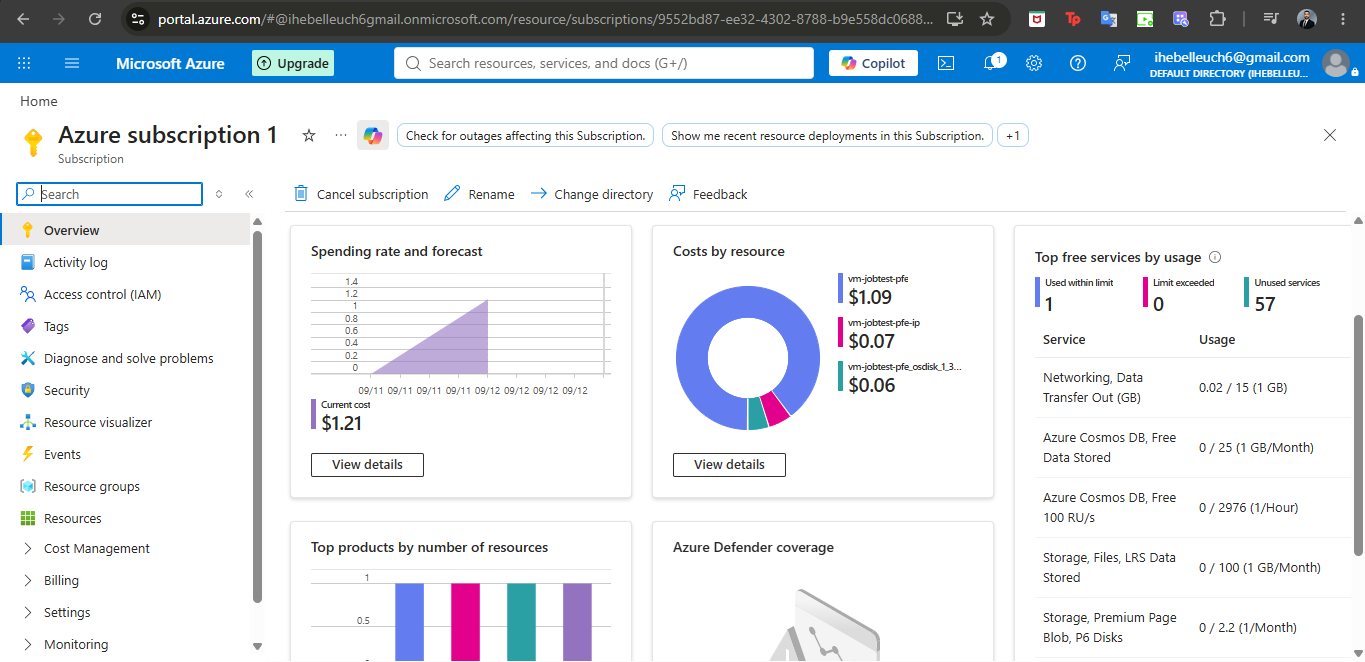
\includegraphics[width=.82\textwidth,trim=0 0 0 105bp,clip]{img/azure/azure_subscription.png}
  \caption{Vue de l'abonnement Azure, recadrée}
  \label{fig:chap6-azure-subscription}
\end{figure}

La figure~\ref{fig:chap6-azure-overview} donne l'aperçu de consommation associé.

\begin{figure}[H]
  \centering
  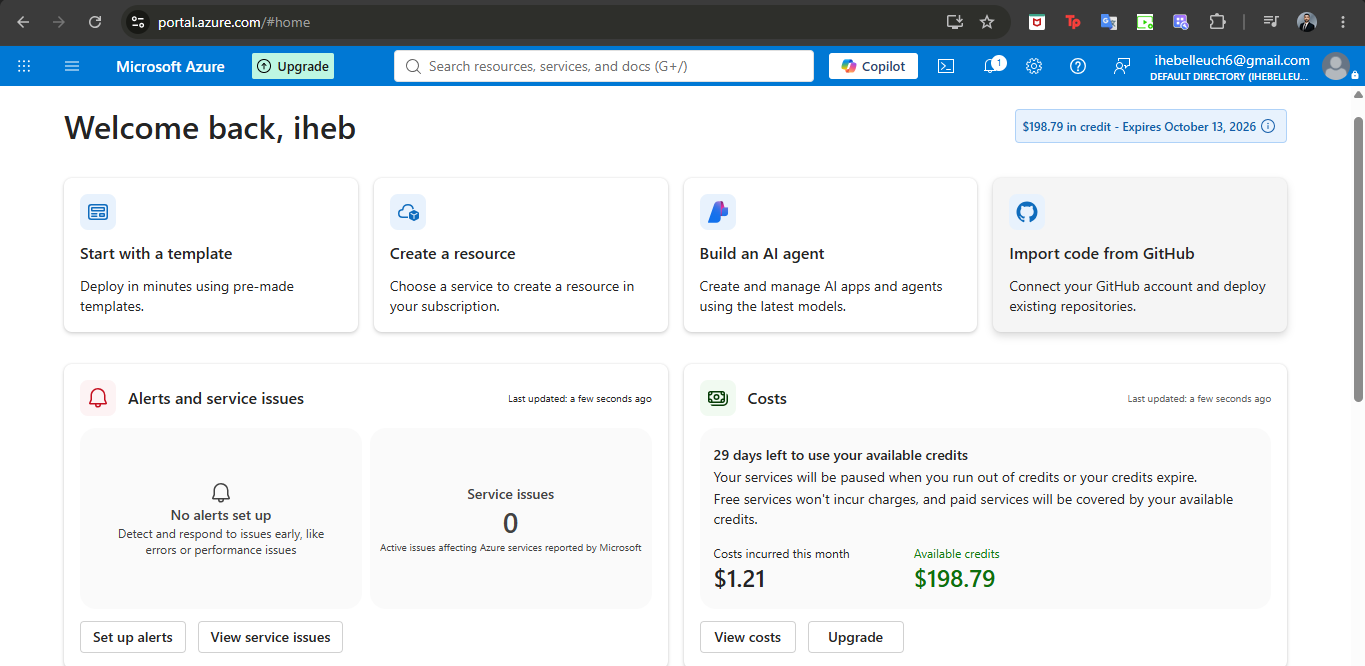
\includegraphics[width=.82\textwidth,trim=0 0 0 170bp,clip]{img/azure/azure_overview.png}
  \caption{Aperçu de consommation Azure, recadré}
  \label{fig:chap6-azure-overview}
\end{figure}

Les ressources créées pour le projet sont visibles sur la figure~\ref{fig:chap6-azure-resources}.

\begin{figure}[H]
  \centering
  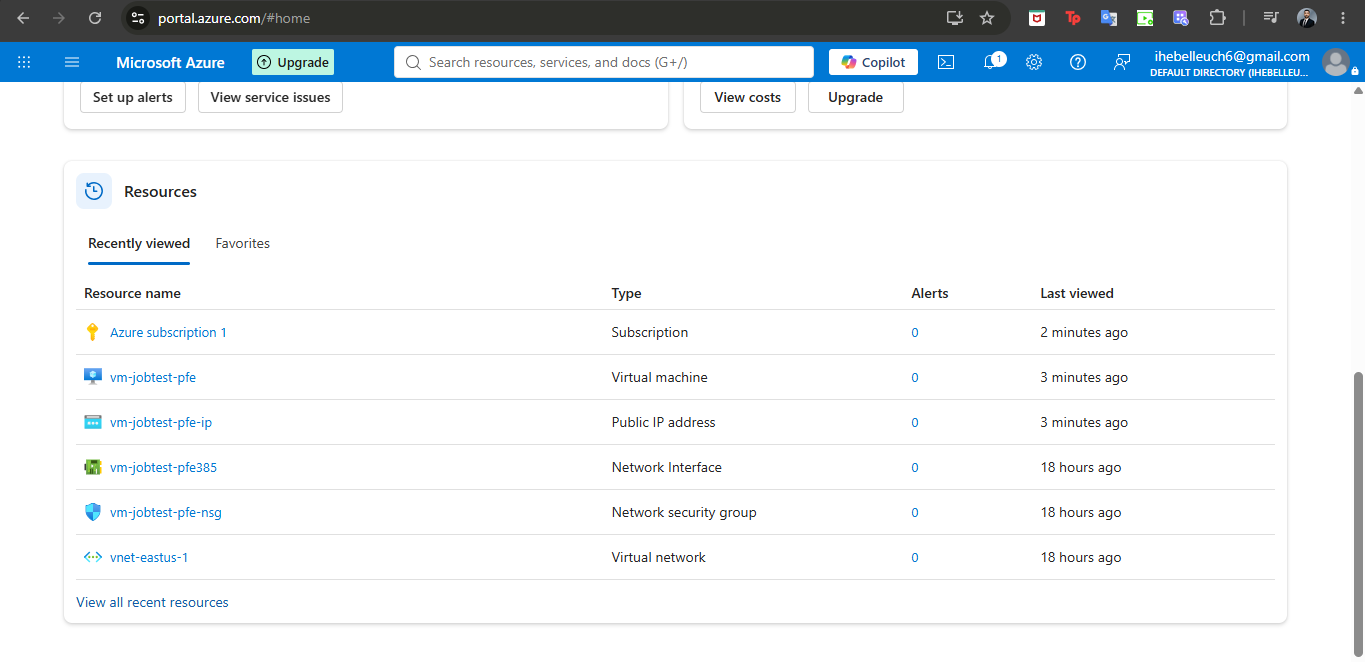
\includegraphics[width=.82\textwidth,trim=0 0 0 105bp,clip]{img/azure/azure_ressources.png}
  \caption{Ressources Azure associées à la démonstration}
  \label{fig:chap6-azure-resources}
\end{figure}

La figure~\ref{fig:chap6-azure-vm-properties} reprend les propriétés de la machine virtuelle.

\begin{figure}[H]
  \centering
  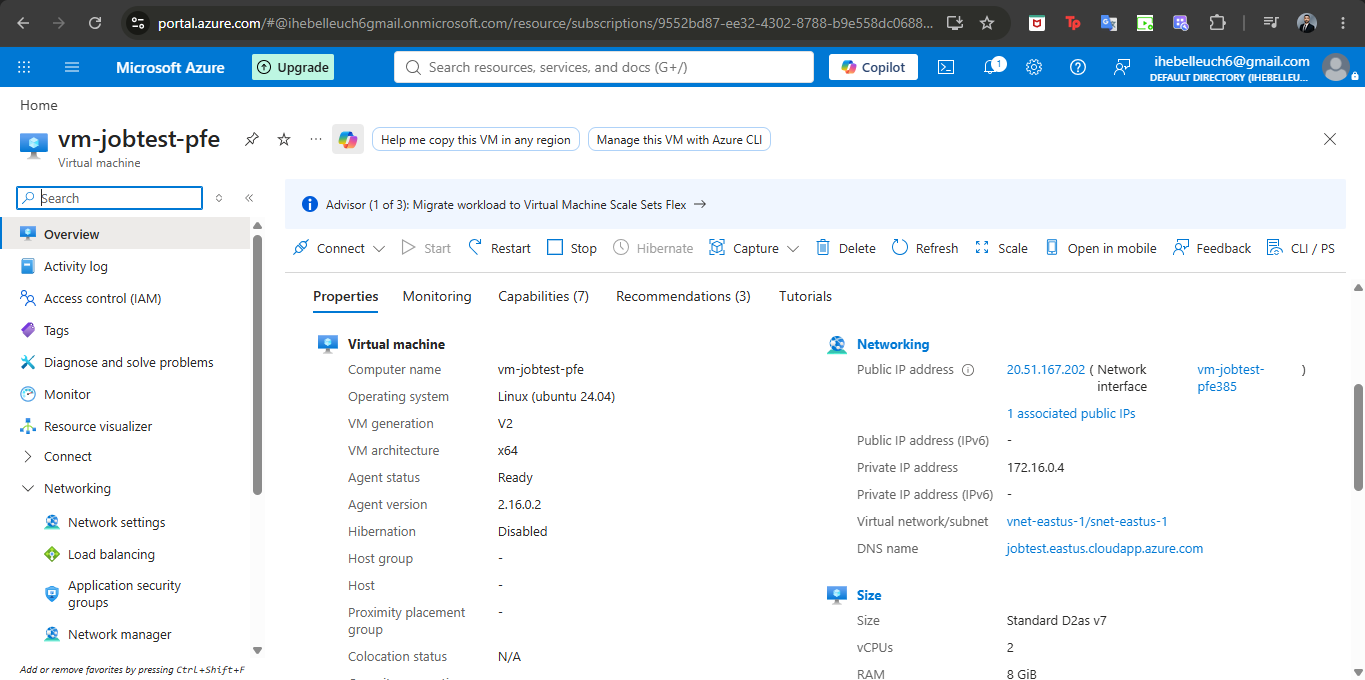
\includegraphics[width=.82\textwidth,trim=0 0 0 105bp,clip]{img/azure/azure_vm1.png}
  \caption{Propriétés observées de la machine virtuelle}
  \label{fig:chap6-azure-vm-properties}
\end{figure}

Son état d'exécution apparaît sur la figure~\ref{fig:chap6-azure-vm-state}.

\begin{figure}[H]
  \centering
  \begin{tikzpicture}[baseline=(image.base)]
    \node[anchor=south west,inner sep=0] (image) at (0,0) {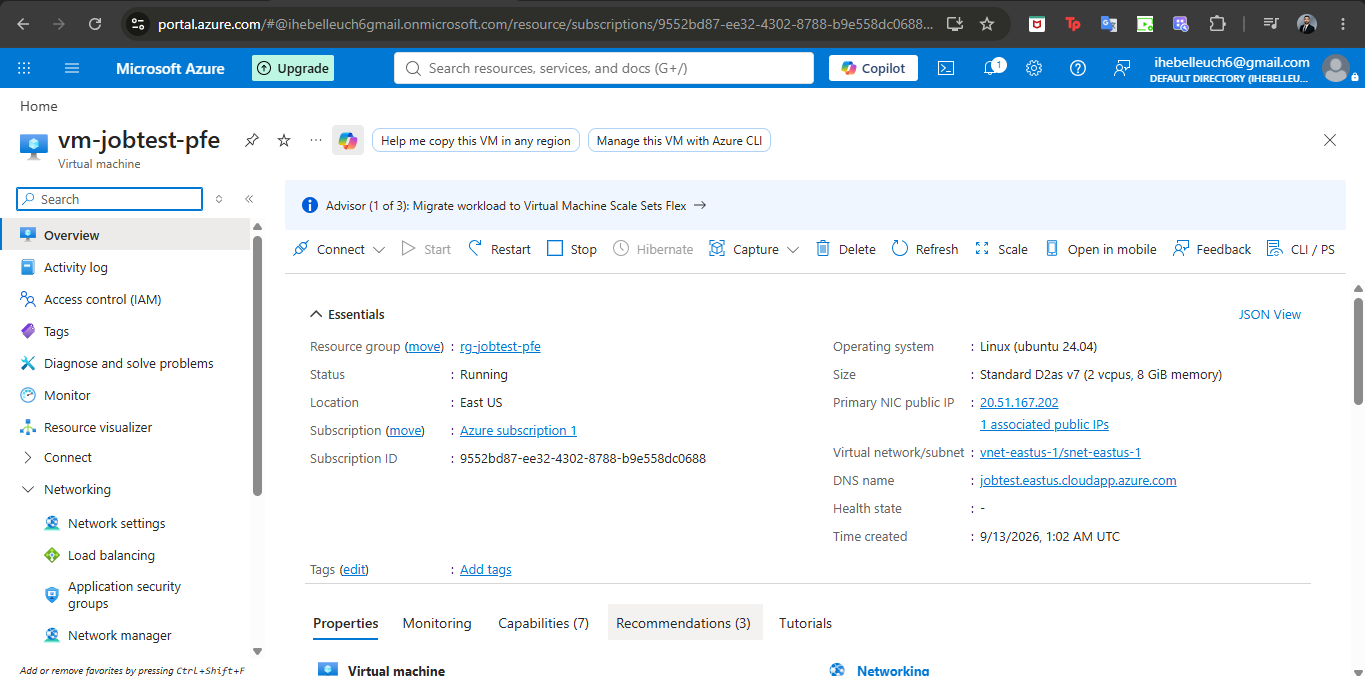
\includegraphics[width=.82\textwidth,trim=0 0 0 105bp,clip]{img/azure/azure_vm2.png}};
    \fill[white] (4.36,2.02) rectangle (8.88,2.63);
    \node[font=\tiny] at (6.62,2.32) {masqué};
  \end{tikzpicture}
  \caption{État de la machine virtuelle, recadré}
  \label{fig:chap6-azure-vm-state}
\end{figure}

La figure~\ref{fig:chap6-azure-ip} montre enfin la ressource d'adresse IP publique rattachée à la machine.

\begin{figure}[H]
  \centering
  \begin{tikzpicture}[baseline=(image.base)]
    \node[anchor=south west,inner sep=0] (image) at (0,0) {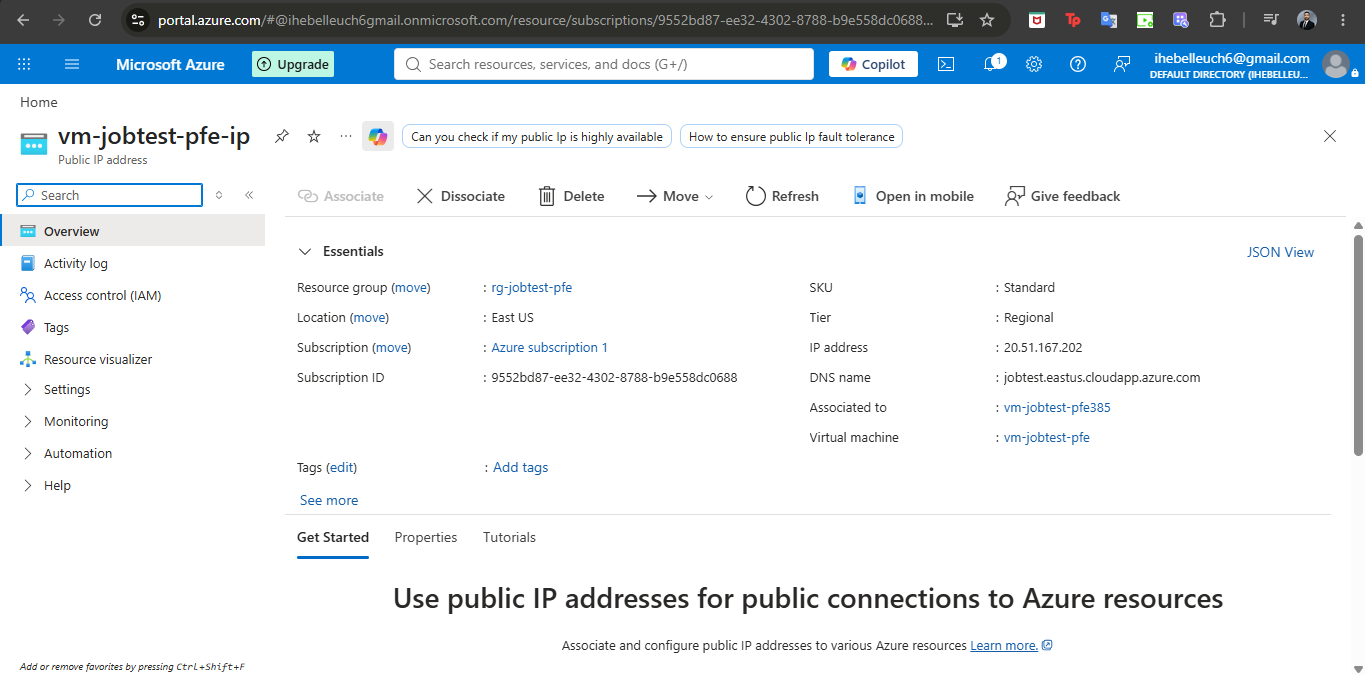
\includegraphics[width=.82\textwidth,trim=0 0 0 105bp,clip]{img/azure/azure ip.png}};
    \fill[white] (4.36,2.53) rectangle (8.88,3.14);
    \node[font=\tiny] at (6.62,2.84) {masqué};
  \end{tikzpicture}
  \caption{Ressource d'adresse IP publique, recadrée}
  \label{fig:chap6-azure-ip}
\end{figure}

Le format D2as\_v7 a été retenu comme compromis pour une démonstration de PFE et pour l'exécution locale de \texttt{qwen2.5:1.5b}. Il n'est pas dimensionné pour une charge réelle soutenue : la latence de la couche 2 sur CPU illustre cette contrainte. La création précise de la règle NSG et son niveau d'attachement n'ont pas été archivés ; seul son effet, l'accès HTTP externe, est confirmé.

\section{Architecture de déploiement}

La figure \ref{fig:chap6-deployment} matérialise les trois frontières utiles à l'exploitation : Azure filtre l'entrée publique, la VM héberge le proxy et le réseau Docker porte les communications de service à service. Les volumes \texttt{postgres\_data}, \texttt{ollama\_data} et \texttt{embedding\_cache} séparent les données persistantes des conteneurs recréables. Le navigateur ne communique ni avec PostgreSQL, ni avec Ollama, ni directement avec FastAPI ou Next.js : il atteint Nginx, qui distribue ensuite les routes internes.

\section{Exploitation et maîtrise des coûts}

Le contexte de démonstration mentionne un crédit Azure Free Trial de 200 USD, sans calcul mensuel figé : le coût affiché dépend de la région, du temps d'allocation et des ressources associées. L'arrêt automatique est activé mais ne doit pas être assimilé sans vérification à une désallocation. Microsoft indique que la fonctionnalité d'auto-arrêt est configurable selon un horaire et un fuseau horaire \cite{azure_auto_shutdown}. Après une démonstration, il faut contrôler l'état réel de la VM et privilégier \emph{Stop (deallocate)} pour libérer le calcul. Le disque et, selon sa configuration, l'adresse IP peuvent continuer à générer des coûts ; la persistance de ces ressources explique qu'une désallocation ne soit pas une suppression.

\section{Procédures d'exploitation}

Les commandes suivantes correspondent aux opérations prévues par la procédure de déploiement. Elles ne révèlent pas le contenu de l'environnement ni les secrets.

\begin{verbatim}
cd /opt/jobtest
docker compose ps
docker compose logs --tail=200 nginx api web ollama db
docker compose restart
docker compose up -d --build
docker compose down
docker compose exec -T db sh -c 'pg_dump -U "$POSTGRES_USER" "$POSTGRES_DB"' | gzip > jobtest-backup.sql.gz
\end{verbatim}

La dernière commande est la forme documentée de sauvegarde PostgreSQL. La commande \texttt{docker compose down} arrête les conteneurs tout en conservant les volumes nommés ; l'option \texttt{-v} n'est donc pas utilisée, car elle supprimerait les données persistantes et les caches.

\section{Bilan du déploiement}

Le tableau~\ref{tab:chap6-deployment-summary} met en regard chaque résultat observé et la limite qui l'accompagne.

\begin{table}[H]
\centering
\small
\caption{Synthèse des résultats observés et des limites}
\label{tab:chap6-deployment-summary}
\begin{tabularx}{\textwidth}{|p{.18\textwidth}|X|X|}
\hline
\textbf{Élément} & \textbf{Résultat observé} & \textbf{Limite}\\
\hline
Interface Next.js & Accessible derrière Nginx. & HTTP uniquement.\\
\hline
API FastAPI & Santé et routes publiques de démonstration disponibles. & Ressources CPU/RAM limitées.\\
\hline
PostgreSQL & Persistance d'un résultat et d'une analyse validée. & Sauvegarde à automatiser.\\
\hline
Couche 1 & Évaluation et explication fonctionnelles. & Validation réelle avec recruteurs encore nécessaire.\\
\hline
Couche 2 & Analyse \texttt{ok} disponible. & Latence CPU élevée ; contenu consultatif.\\
\hline
PDF & Export valide sur un exemple de deux pages. & Test ponctuel, taille variable.\\
\hline
Réseau & Ports applicatifs internes non publiés. & SSH à restreindre ; UFW inactif observé.\\
\hline
Disponibilité & Démonstration réussie avec cinq services sains. & VM unique, sans haute disponibilité.\\
\hline
\end{tabularx}
\end{table}

\section*{Conclusion}

Les preuves réunies confirment le fonctionnement d'une chaîne complète de démonstration : l'évaluation, la persistance, l'analyse qualitative et l'export PDF sont servis par une pile conteneurisée, avec Nginx comme point d'entrée et des services métier non publiés directement. Le déploiement Azure est donc opérationnel dans son périmètre de PFE. Il ne constitue toutefois ni une certification de sécurité ni une infrastructure de production : HTTPS, le durcissement de SSH, les sauvegardes, la supervision et la tolérance aux pannes restent à mettre en œuvre. Ces résultats permettent de replacer, dans la conclusion générale, les apports du prototype et les conditions de son évolution.

        \clearpage
        \chapter*{Conclusion générale}
\addcontentsline{toc}{chapter}{Conclusion générale}
\markboth{Conclusion générale}{}

Le recrutement confronte les organisations à un volume important de CV, à des offres exprimées de manière hétérogène et à la nécessité de justifier un premier tri. Dans ce contexte, rapprocher automatiquement un CV et une offre ne doit pas réduire une candidature à un classement opaque. Le besoin auquel répond JobTest est celui d'une aide structurée~: mettre en évidence les éléments de compatibilité, les écarts et les raisons d'une recommandation, tout en laissant au recruteur la décision finale.

Le projet avait pour objectif de concevoir et réaliser une plateforme Web d'aide au recrutement capable de gérer les offres, les candidats et leurs CV, de produire une évaluation hybride, d'en restituer une explication et d'en préserver la traçabilité. La solution livrée propose un frontend Next.js, une API FastAPI, une persistance SQLAlchemy utilisant SQLite en développement et PostgreSQL dans l'environnement conteneurisé, ainsi qu'un export PDF. Le recruteur peut créer ses offres, gérer ses candidats, lancer une évaluation, consulter son historique et obtenir un rapport. Les contrôles d'appartenance des données maintiennent la séparation entre les espaces des recruteurs.

La démarche a suivi les étapes de l'étude du contexte, de l'analyse des besoins, de la conception UML et architecturale, du développement, de la conception du moteur de rapprochement, puis de la validation et du déploiement. Elle s'inscrit dans le cycle en cascade présenté au début du rapport, tout en intégrant les retours techniques nécessaires au fil des vérifications. L'industrialisation a complété le développement par Docker Compose, un proxy inverse comme point d'entrée et un déploiement de démonstration sur une VM Microsoft Azure, servi en HTTPS.

La contribution centrale est un moteur hybride qui combine les signaux TF--IDF, sémantique et compétences, contrôle les preuves présentes dans le CV, calibre son score puis applique des règles de décision explicites. Le score est reproductible, versionné et s'accompagne de sous-scores, de forces, de lacunes et de recommandations structurées. Un CV qui recopie les exigences de l'offre ou qui ne fait que les lister n'obtient pas le verdict \texttt{HIRE}. Une seconde couche locale, exécutée avec Ollama, produit une analyse qualitative séparée~: elle enrichit la lecture du recruteur, mais ne peut ni modifier le score officiel ni déterminer seule la recommandation algorithmique \texttt{HIRE}, \texttt{CONSIDER} ou \texttt{REJECT}. Cette séparation est un résultat important du projet, car elle maintient une distinction claire entre calcul déterministe et contenu génératif.

Les validations réunies montrent que le parcours complet fonctionne~: authentification, création d'offre, évaluation d'un texte ou d'un document, persistance, analyse approfondie et génération PDF. Je l'ai exercé sur des données synthétiques, sur des CV fictifs au format PDF et sur mes propres CV face à des offres réelles. Le déploiement a également confirmé les cinq services conteneurisés, le proxy inverse, l'accès HTTPS et l'isolation des ports métier du réseau public. Sur le test synthétique isolé, les verdicts affichés par la version finale atteignent un macro-F1 de 0,740 sur trois classes, sans dépasser TF--IDF seul calibré. Ces mesures restent internes au corpus synthétique~; les essais menés avec mes propres CV, faute de jugements de référence indépendants, restent qualitatifs. La valeur démontrée est celle d'un prototype fonctionnel et traçable, non celle d'un système déjà validé en situation opérationnelle.

Cette prudence est essentielle. Le jeu d'évaluation quantitative est synthétique, les ancrages de calibration sont appris sur ses étiquettes, les poids restent fixés empiriquement, le dictionnaire de compétences est nécessairement incomplet et aucune annotation par des recruteurs n'a été réalisée. Un CV qui décrit faussement une expérience n'est pas détecté par l'analyse du texte. Les biais possibles dans les données, les libellés ou les règles doivent être étudiés avant tout usage réel. La couche 2 présente une latence notable sur CPU et son texte, bien que contrôlé par des statuts, reste consultatif. Du point de vue de l'infrastructure, la démonstration est hébergée sur une VM unique, sans haute disponibilité, sans sauvegarde automatisée ni supervision avancée. Une politique explicite de protection, de conservation, d'anonymisation et de suppression des CV demeure également indispensable.

Les évolutions prioritaires à court terme sont la sécurisation des sessions par cookies adaptés, la restriction de SSH, les sauvegardes PostgreSQL, le monitoring et la correction des limites de téléversement. L'amélioration de l'interface et l'optimisation de la couche 2 peuvent progresser en parallèle. À moyen terme, il sera nécessaire de confronter le système à un corpus réel anonymisé et autorisé, de travailler avec des recruteurs, d'enrichir le dictionnaire de compétences, de réapprendre la calibration du score sur ces données annotées, ce qui constitue la priorité, d'évaluer les biais et de formaliser l'évaluation des explications génératives, y compris dans plusieurs langues.

À plus long terme, une charge réelle justifierait des traitements asynchrones, une file de tâches, une meilleure observabilité et, si nécessaire, la séparation de certains services sur une infrastructure évolutive. Des intégrations avec des systèmes de gestion de recrutement pourraient être envisagées, accompagnées de mécanismes de gouvernance et d'audit des décisions assistées. Ces perspectives ne sont pas des fonctions déjà réalisées~; elles dessinent les conditions d'une évolution responsable.

JobTest constitue ainsi un prototype fonctionnel et une base technique cohérente pour l'aide à l'analyse des candidatures. Il organise des signaux et des explications utiles au recruteur, sans prétendre remplacer son jugement, l'appréciation du contexte ou sa responsabilité dans la décision finale.

        \clearpage
        
        % @author: Stoufa
		% the command `\nocite{*}` is mandatory to avoid the “no \citation commands” error
        % https://tex.stackexchange.com/questions/18045/problem-with-compiling-bibtex-no-citation-commands-error
        %\nocite{*}
        % Keeps the last table-of-contents entries on the same page instead of
        % leaving a single line alone on an extra page.
        \addtocontents{toc}{\protect\enlargethispage{2\baselineskip}}
        \printbibliography[heading=bibintoc]
        \clearpage
        \chapter*{Résumé}
\addcontentsline{toc}{chapter}{Résumé}
\markboth{Résumé}{}

Ce mémoire présente JobTest, une plateforme Web d'aide à la présélection qui rapproche des CV et des offres d'emploi. La solution combine des signaux TF--IDF, sémantiques et de compétences, contrôle les preuves présentes dans le CV, calibre le score obtenu, applique une décision explicite et restitue ses composantes au recruteur. Elle intègre un frontend Next.js, une API FastAPI, une persistance relationnelle, un export PDF et une analyse générative locale optionnelle, séparée du verdict officiel. Les validations couvrent les parcours principaux, un banc d'essai quantitatif sur données synthétiques, des essais fonctionnels avec des CV fictifs et avec mes propres CV, ainsi qu'un déploiement de démonstration conteneurisé sur Azure. Sur le test synthétique, les verdicts affichés atteignent un macro-F1 de 0,74 sur trois classes ; la calibration doit encore être réapprise sur des données réelles annotées. JobTest assiste le recruteur sans remplacer son jugement ni une décision humaine.

\noindent\textbf{Mots-clés :} recrutement, appariement CV-offre, IA explicable, FastAPI, Next.js.

\chapter*{Abstract}
\addcontentsline{toc}{chapter}{Abstract}
\markboth{Abstract}{}

This thesis presents JobTest, a web platform that assists recruiters in matching resumes with job offers. The solution combines TF--IDF, semantic and skill-based signals, screens the evidence contained in the resume, calibrates the resulting score, applies an explicit decision policy, and exposes the components of the result to the recruiter. It includes a Next.js frontend, a FastAPI API, relational persistence, PDF export, and an optional local generative analysis that is kept separate from the official verdict. The validation covers the main user flows, a quantitative benchmark on synthetic data, functional trials with fictitious resumes and with my own resumes, and a containerized demonstration deployment on Azure. On the synthetic test set, the displayed verdicts reach a three-class macro-F1 of 0.74; the calibration still has to be re-fitted on annotated real data. JobTest supports recruiters without replacing their judgement or human decision-making.

\noindent\textbf{Keywords:} recruitment, CV-job matching, explainable AI, FastAPI, Next.js.

\vfill
\begin{center}
\textbf{Démonstration de JobTest}\\[3mm]
\qrcode[height=3.2cm]{https://jobtest-pfe-iheb.eastus.cloudapp.azure.com/login}\\[2mm]
\url{https://jobtest-pfe-iheb.eastus.cloudapp.azure.com/login}\\[2mm]
\begin{minipage}{.8\textwidth}\centering\footnotesize
Instance de démonstration hébergée sur Microsoft Azure et servie en HTTPS, sans garantie de disponibilité permanente. N'y saisir que des données fictives.
\end{minipage}
\end{center}

        
\end{document}
